\chapter{泥岩流变力学特性试验研究}
\label{chap:theory}
流变特性作为岩石最重要的力学性质之一,与岩土工程的长期稳定性和安全性密切相关。
为了深入分析山体与其内部隧道相互作用下的变形时效特性,必须对岩石进行流变
力学试验,得出岩石流变行为及破坏规律,为岩石流变本构模型的建立奠定基础。在进行流变试验之前,需要对其进行常规三轴压缩试验,根据压缩试验得到的该种岩石基本的抗压强度和变形特性,设计进行相应的三轴流变试验,得出岩石流变行为及破坏规律,为岩石流变本构模型的建立奠定基础。
本节主要介绍三轴流变试验的过程及数据分析。
为了开展。。。。。。。研究,获取参数,针对xxxx的岩石,开展了xxx的实验。本章对实验的过程和结果进行了阐述。

%\section{工程地质概况}

%流变特性作为岩石最重要的力学性质之一,与岩土工程的长期稳定性和安全性密切相关。
%为了深入分析山体与其内部隧道相互作用下的变形时效特性,必须对岩石进行流变
%力学试验,得出岩石流变行为及破坏规律,为岩石流变本构模型的建立奠定基础。在进行流变试验之前,需要对其进行常规三轴压缩试验,根据压缩试验得到的该种岩石基本的抗压强度和变形特性,设计进行相应的三轴流变试验,得出岩石流变行为及破坏规律,为岩石流变本构模型的建立奠定基础。
%

\section{试样及试验仪器简介}
本文以xxx为研究背景,选取xxx的泥岩为研究对象,试验所需试样均为现场直接钻芯所得。将岩样制作成直径\SI{50}{mm}、高度\SI{100}{mm}标准试样,试
件满足两端面不平行度误差不大于\SI{0.05}{mm}、沿高度方向直径误差不大于\SI{0.03}{mm}以及端面与试件轴线的最大偏差不大于\SI{0.25}{\degree}等要求,现场钻取的岩芯以及制作好的试样分如图~\ref{fig:2-1}所示。

\begin{figure}[ht!]
    \centering
    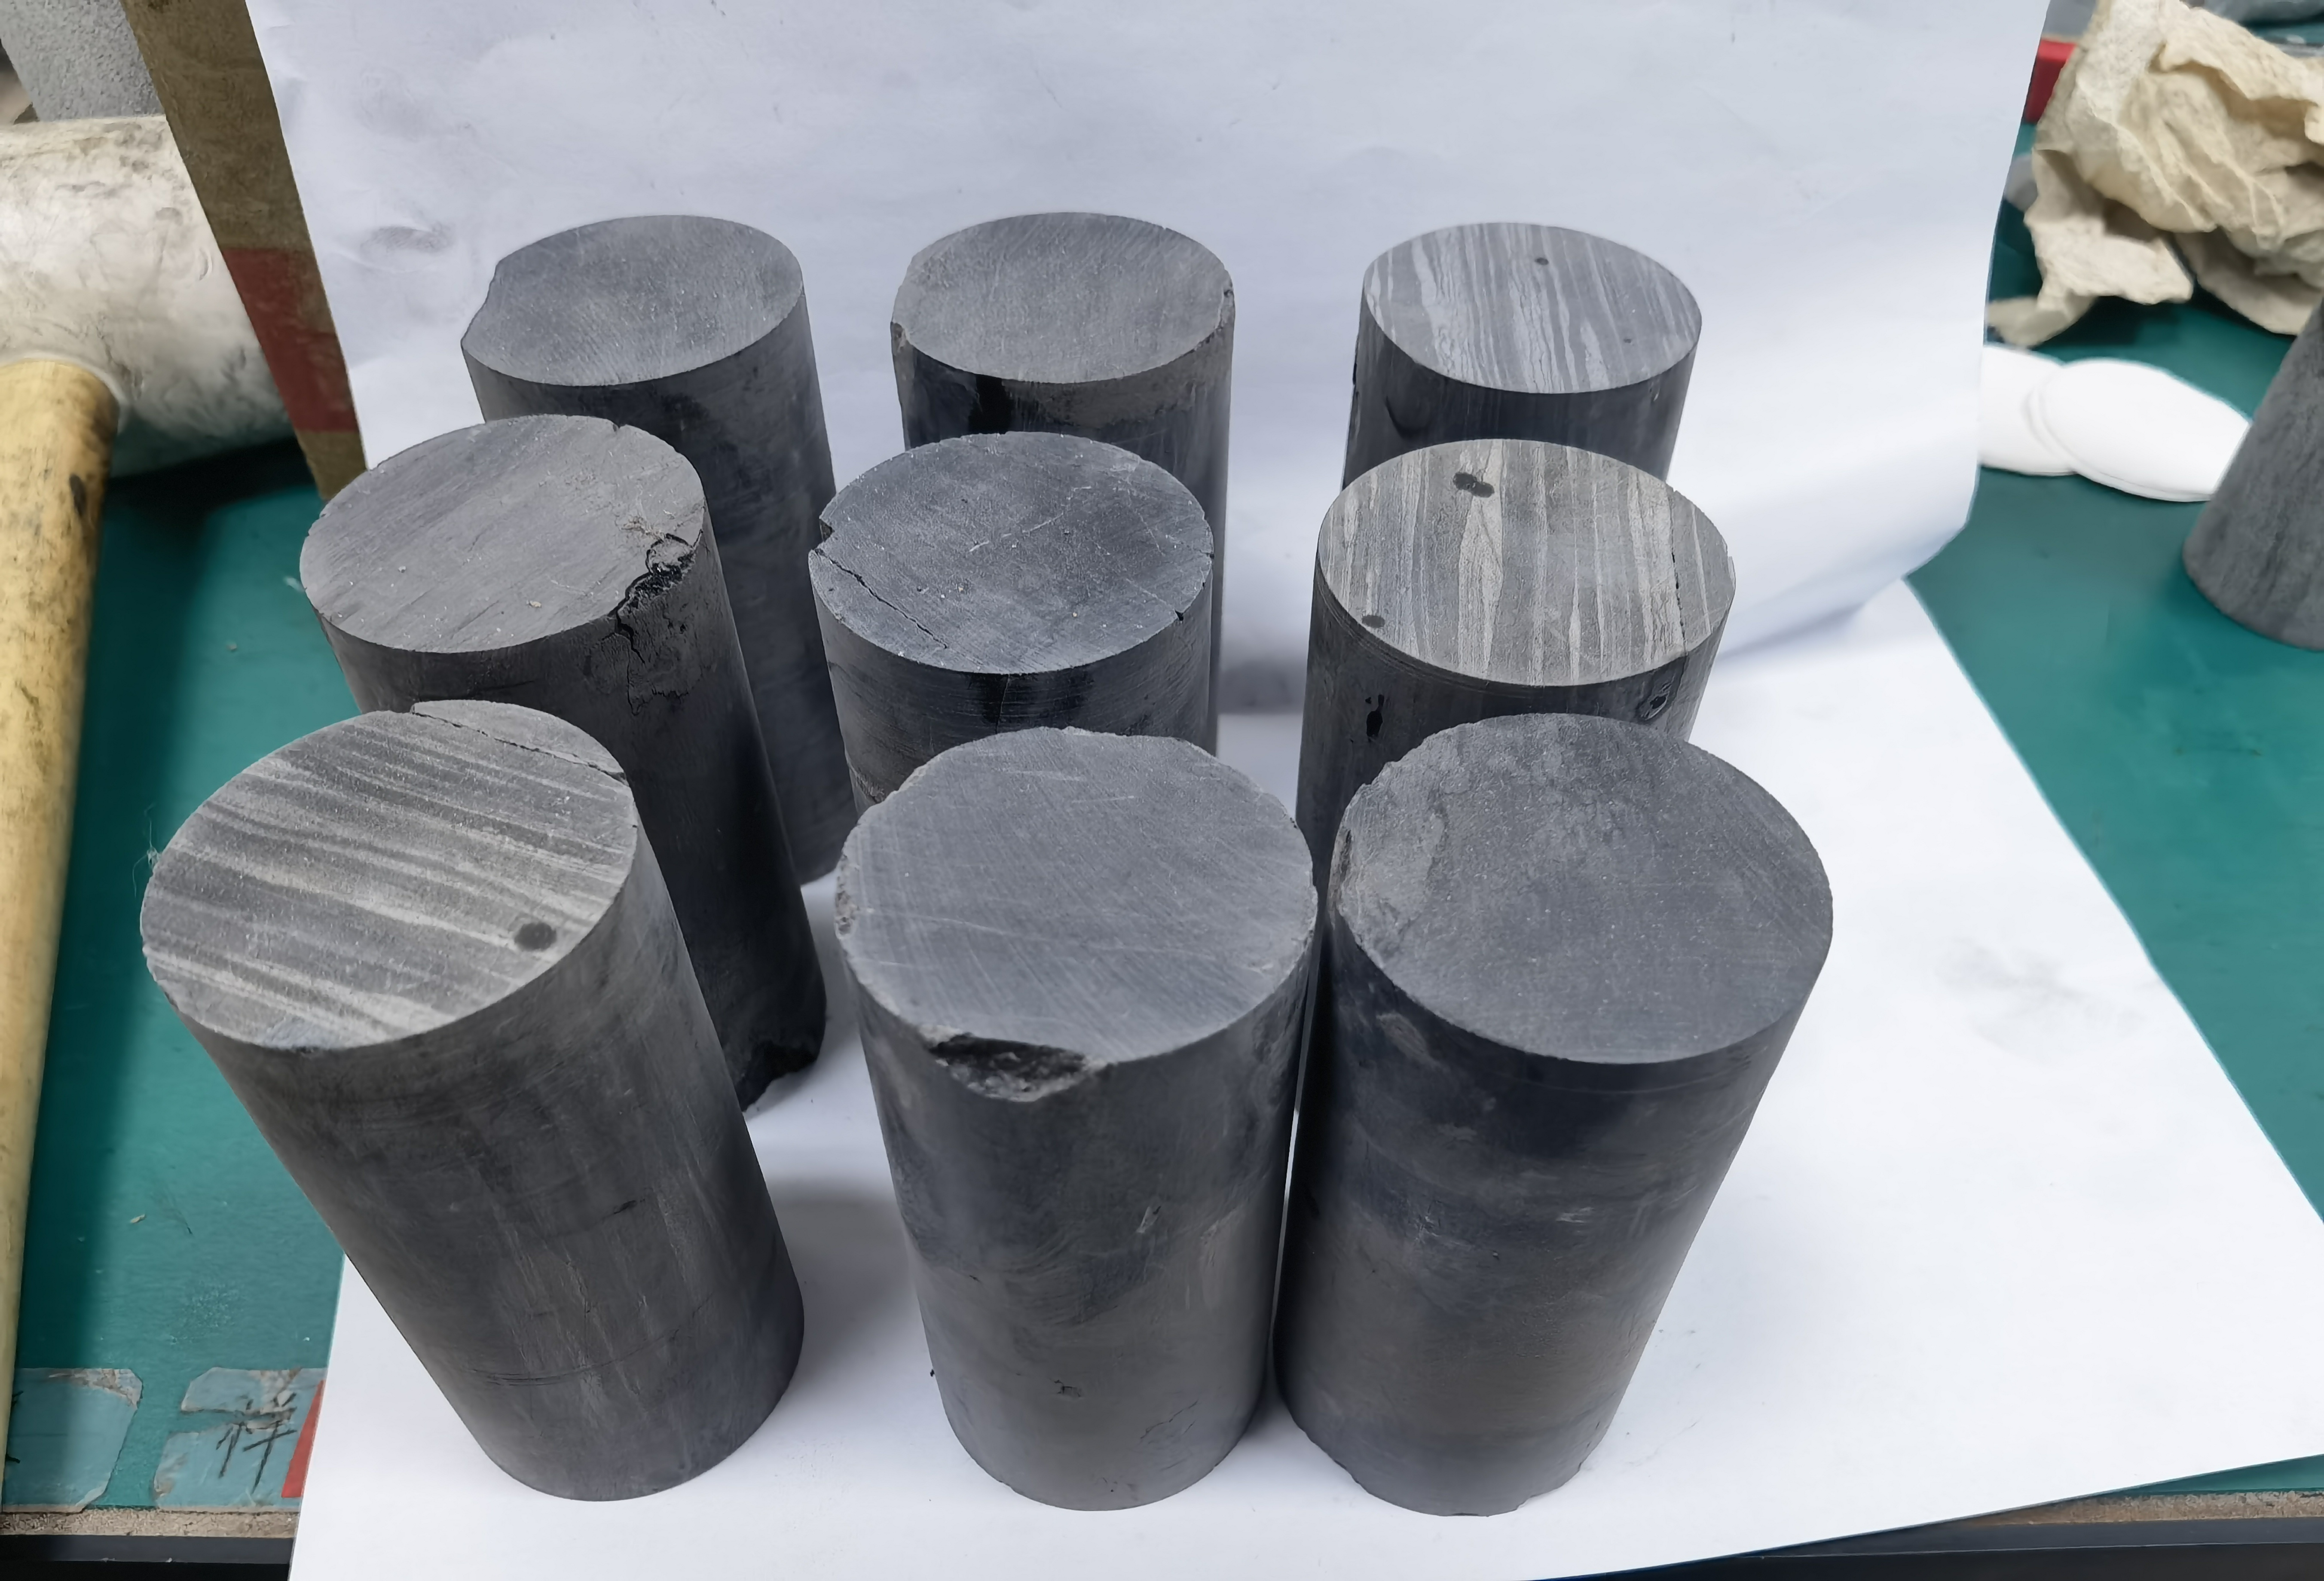
\includegraphics[width=0.5\textwidth]{img/chap2/试样制备.jpg}
    \caption{泥岩试样}
    \label{fig:2-1}
\end{figure}

本次试验在多尺度多场耦合岩石力学试验室完成,使用的设备为法国TOP Industrie公司生产三轴流变仪(如图2.2所示)和气体渗透控制面板。

三轴流变仪于2016年12月完成安装测试,设计最大压力室工作围压为\SI{150}{MPa},最大工作孔压为\SI{150}{MPa},轴向压力最大可达200吨。该设备主要由三轴压力室、轴压伺服泵、围压伺服泵、水压伺服泵、气渗系统、加热装置、超声波测试系统和计算机控制系统组成,可实现岩石常规三轴压缩试验、流变试验、渗透试验以及温度-流体-力学-化学等多场耦合试验,适用范围广,测量精度高。压力控制采用高精度电控伺服高压泵,测量精度可达\SI{0.01}{MPa};轴向位移测量使用两只高灵敏度的位移传感器,可直接输出被测试样的轴向位移值,量程20mm,测量精度达\SI{e-3}{mm};径向位移测量使用应变片式侧向应变仪,输出全桥电路压敏电阻的电压变化值,换算求得径向应变,测量精度达\SI{e-3}{mv/v}。该系统可实现多种方式加载压力,其中轴向压力可选择轴向位移控制、压力控制、流量控制、环向位移控制等加载方式。

\begin{figure}[ht!]
    \centering
    \subfigure[系统图]
    {
        \begin{minipage}{8.6cm}
            \centering
            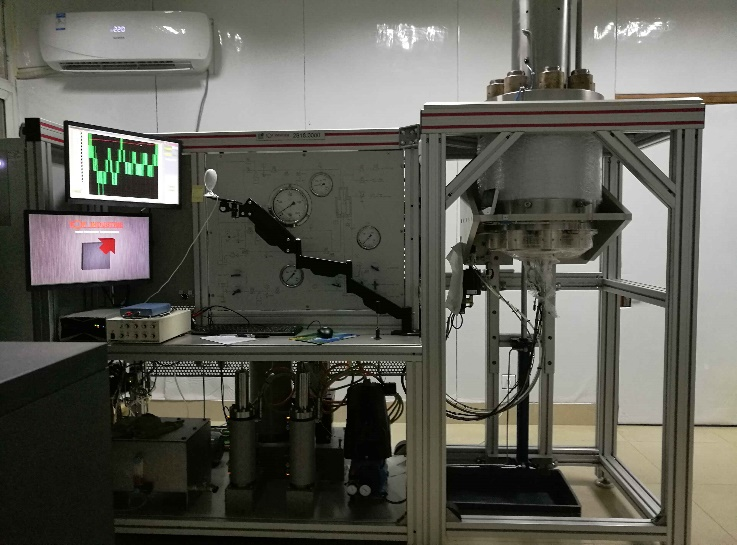
\includegraphics[width=0.9\textwidth]{img/chap2/Multi-scale and multi-field coupling triaxial tester-1.png}
        \end{minipage}
    }
    \subfigure[围岩室]
    {
        \begin{minipage}{5.3cm}
            \centering
            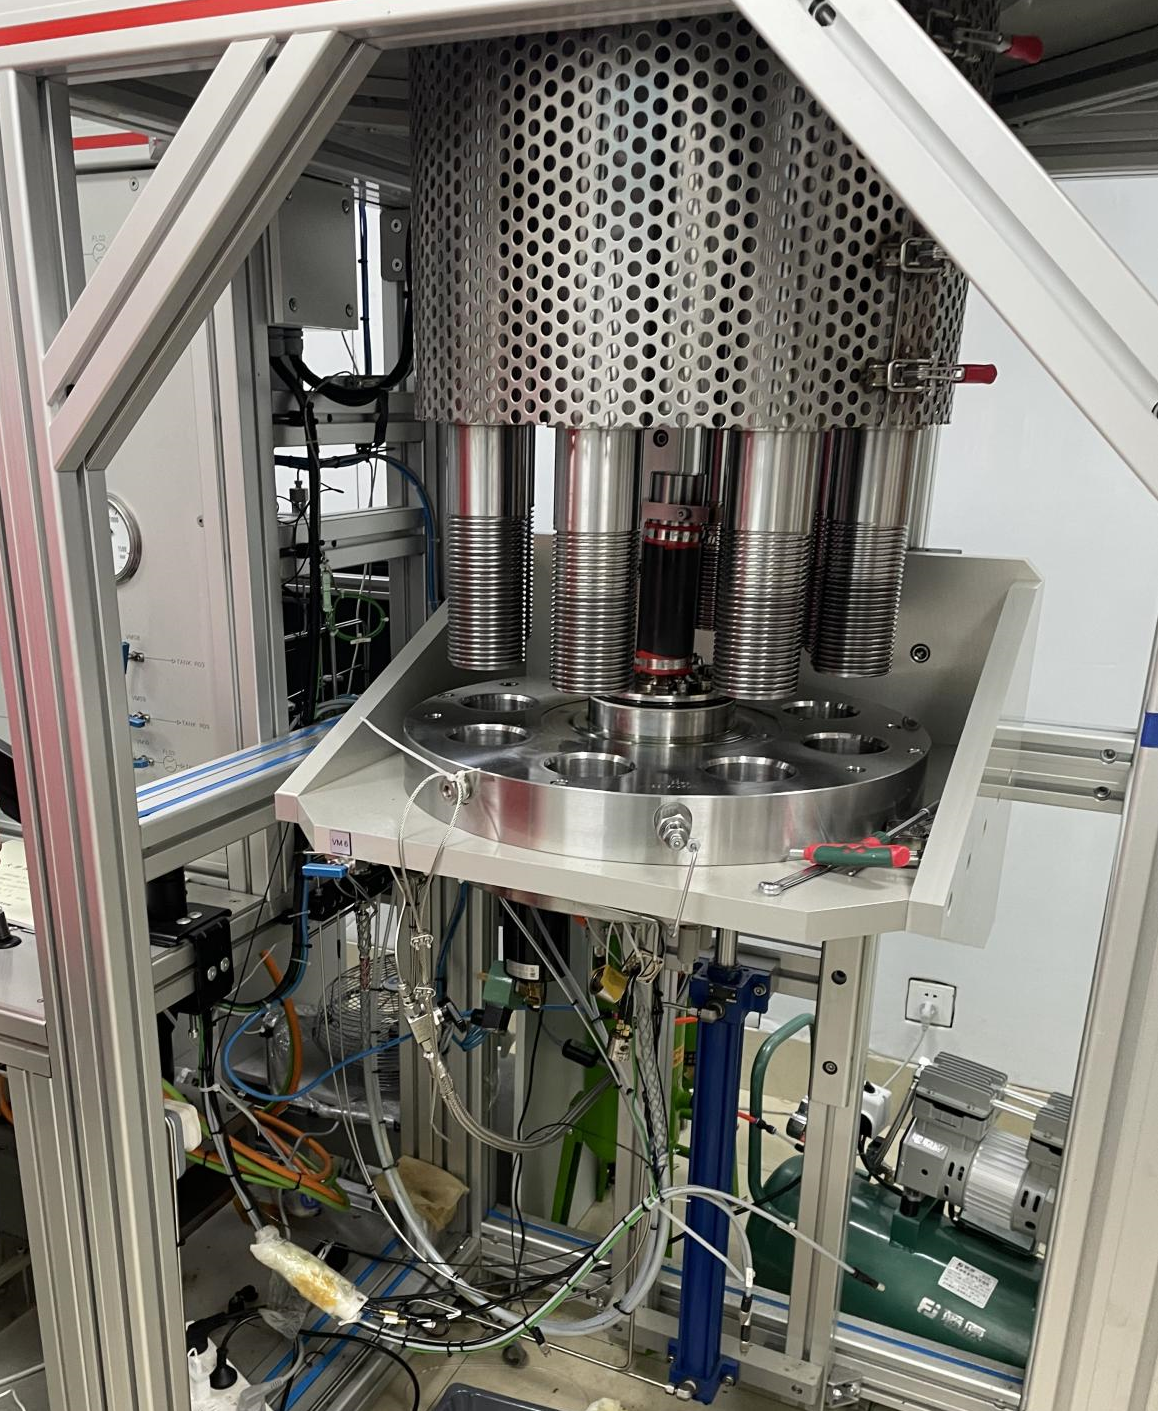
\includegraphics[width=0.9\textwidth]{img/chap2/Multi-scale and multi-field coupling triaxial tester-2.png}
        \end{minipage}
    }
    \caption{多尺度多场耦合三轴试验仪}
    \label{fig:2-2}
\end{figure}

\section{实验方案}

%为什么开展,单轴,三轴,及单三轴流变,方案列表。

\section{泥岩单/三轴压缩实验}
\subsection{试验过程}\label{section:试验过程}
试样三轴压缩试验方案和步骤如下:

(1)试样选取及测量:首先剔除外观有明显缺口、裂缝和节理的试样,选取均质性较好的试样,确定初步筛选后的试样的基本几何和物理参数,包括试样的长度、直径、质量等,通过计算得到密度。试样尺寸的测量采用\SI{0.01}{mm}精度的游标卡尺,在三个不同的位置测量然后取平均值;试样质量的测量使用\SI{0.01}{g}精度的天平,称重三次取平均值,完成后对试样进行编号(如图~\ref{fig:2-3});

(2)试样安装:将试样套入内径\SI{50}{mm}的橡皮套中后将其放置在底座上,试样两端需各放置一片滤纸用于防止试样破坏后的岩石碎屑进入底座的气体通道。之后将压头套入橡皮套放置于试样顶部,橡皮套两端用小宽度喉箍固定密封,防止围压室的液压油进入橡皮套;

(3)充油加围压:本次三轴试验的围压为\SI{5}{MPa}、\SI{10}{MPa}、\SI{15}{MPa}三个等级。首先密封压力室,用低压泵向压力室内充油,再用围压泵将围压加至试验设定的围压值,并维持恒定,围压加载速率为\SI{3}{MPa/min},加载到预定的围压等级后停止加载;

(4)接触加偏应力:围压加载完成后可进行施加偏应力,需要指出的是在施加偏应力前,必须将试样与三轴伺服仪轴压压头进行接触,可手动操作向轴压压力室加油,待轴向应变变化说明已经接触,且接触后要卸载此时的偏应力值到零,最后加满轴压泵,采用速度加载方式,设置大于岩石预估最大偏应力的轴向应力上限值,加载速率设置为\SI{0.02}{mm/min},加载至试样破坏;

(5)待试验全部完成后将气体面板和进气口阀门关闭,将偏压卸载至\SI{0}{MPa},再将围压卸至\SI{0}{MPa},排油结束后即可拆样进行下一步实验。

对于单轴压缩实验而言,试验方案与步骤与上述三轴压缩试验步骤基本一致,只是在试样安装完毕后,不需要通过油泵对试样充油施加围压,直接施加轴向应力即可。

后续试验需要确定泥岩试样的基本变形特性和抗压强度值,在明确了以上目的后,
我们对试样设计、进行了单轴和三轴压缩试验。考虑到一组试验测得的数据可能存在偶然性和较大的误差,因此单轴压缩试验共计进行了三组,我们对三组试验获得的抗压强度求平均值,以此平均值作为后续单轴流变试验的基础强度值。而三轴压缩试验因为时间和试样数量所限,只在每种围压下完成一个试样的试验,具体试验方案如下表~\ref{tab:泥岩三轴压缩试验工况表}

\begin{figure}[ht!]
    \centering
    \subfigure[试样编号]
    {
        \begin{minipage}{7cm}
            \centering
            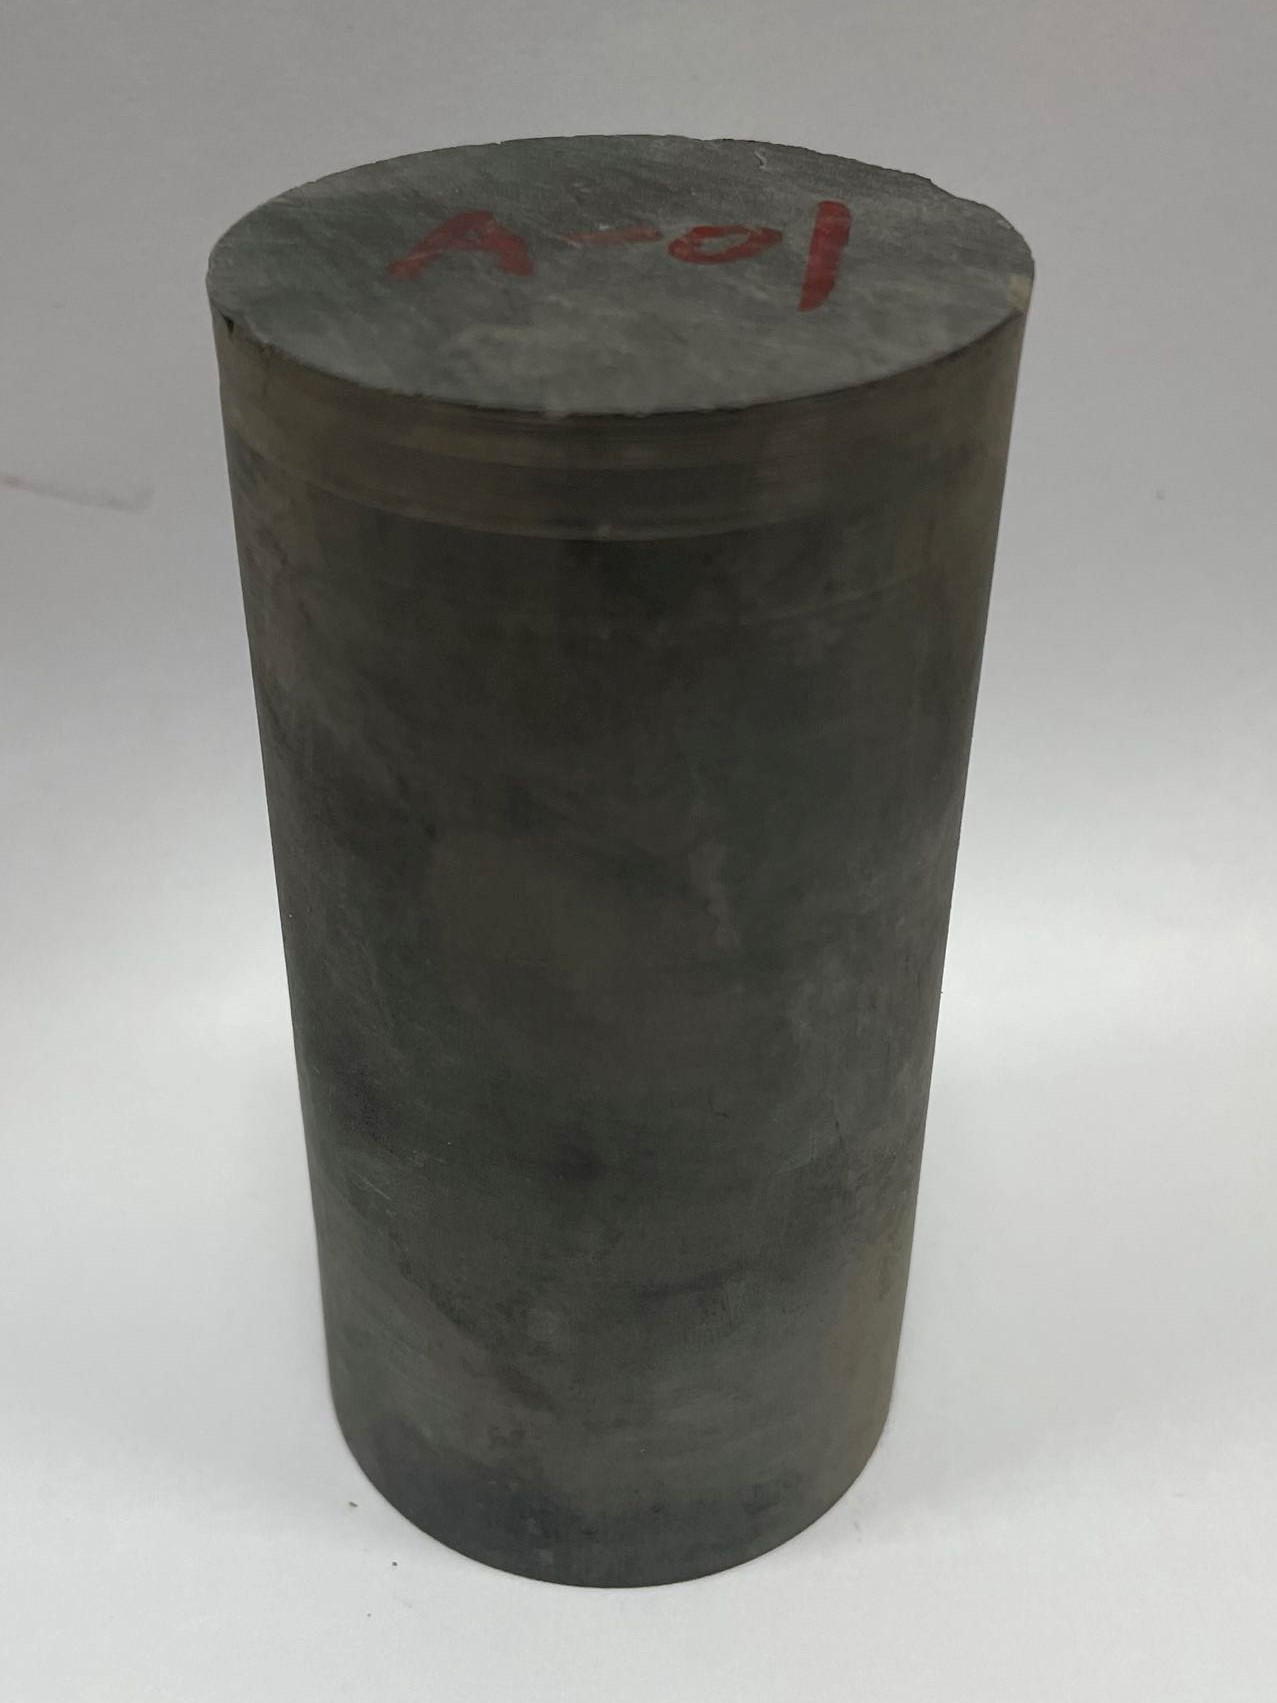
\includegraphics[width=0.9\textwidth]{img/chap2/试样编号.png}
        \end{minipage}
    }
    \subfigure[试样放置]
    {
        \begin{minipage}{7cm}
            \centering
            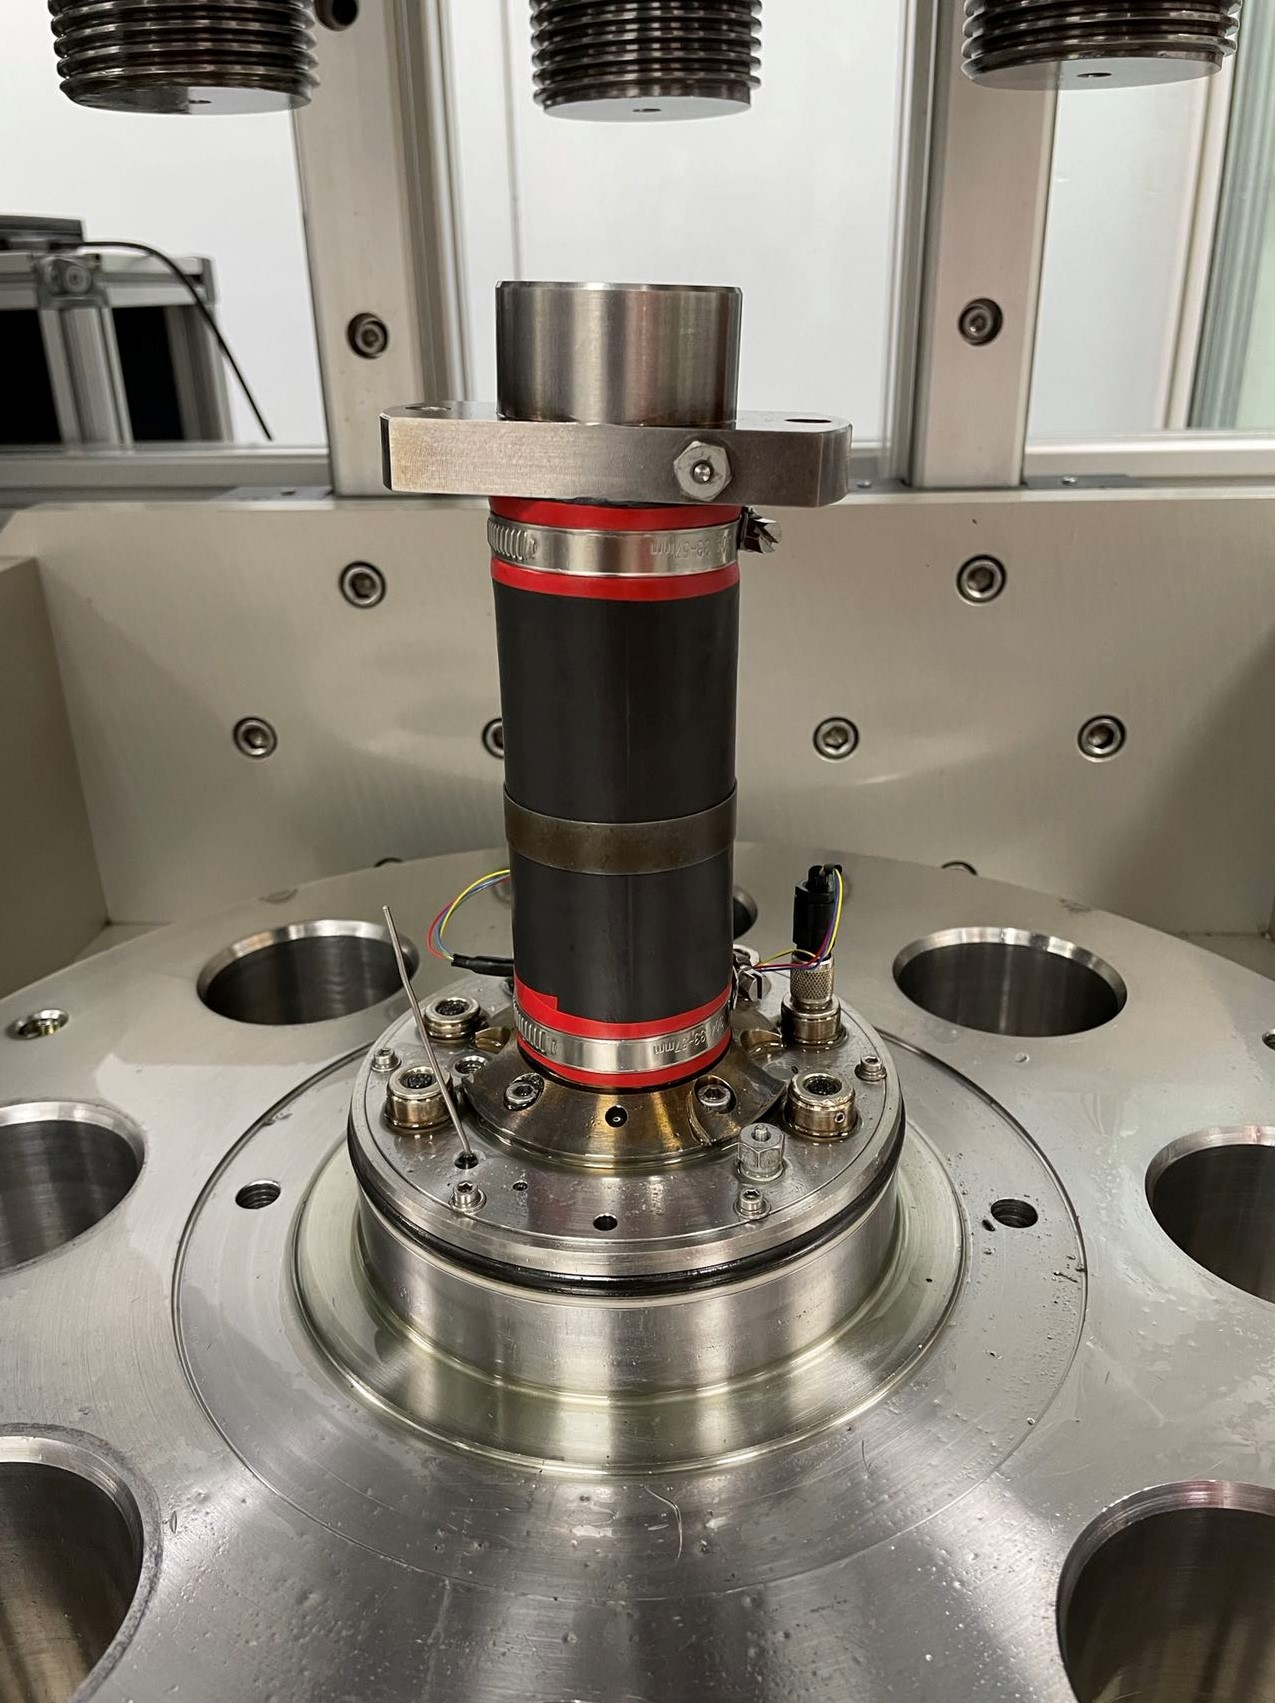
\includegraphics[width=0.9\textwidth]{img/chap2/试样放置.png}
        \end{minipage}
    }
    \caption{试验步骤}
    \label{fig:2-3}
\end{figure}


在本次试验计划中,进行泥岩的单轴压缩及三轴压缩试验,一是为了通过压缩试验获得泥岩的应力-应变曲线,并据此分析泥岩试样的基本力学参数、强度特征及变形特征;二是为了获得试样的抗压强度值,为后续的流变试验做好准备。



\begin{table}[ht!]\small
    \centering
    \begin{tabular}{p{3cm}<{\centering} p{3cm}<{\centering} p{3cm}<{\centering} p{3cm}<{\centering}}
        \toprule
        试样编号  & 围压(MPa)  &  试样高度h(mm)   &  试样直径d(mm)\\
        \midrule
        A-01        & 0  &   98.47  &  50.10   \\ 
        A-02        & 0  &   99.17  &  49.29   \\ 
        A-03        & 0  &   99.82  &  50.16  \\ 
        \midrule
        B-01        & 5  &   99.86  &  49.30    \\ 
        B-02        & 10 &   100.31 &  49.83    \\ 
        B-03        & 15 &   99.78  &  49.74 \\ 
        \bottomrule
    \end{tabular}
    \caption{泥岩三轴压缩试验工况表}
    \label{tab:泥岩三轴压缩试验工况表}
\end{table}



\subsection{试样破坏特征分析}
泥岩试样在不同的围压水平下表现出不同的破坏形态,下图展示了进行三轴压缩试验的试样破坏后的形态:
\begin{figure}[ht!]
    \centering
    \subfigure[A-01]
    {
        \begin{minipage}{7cm}
            \centering
            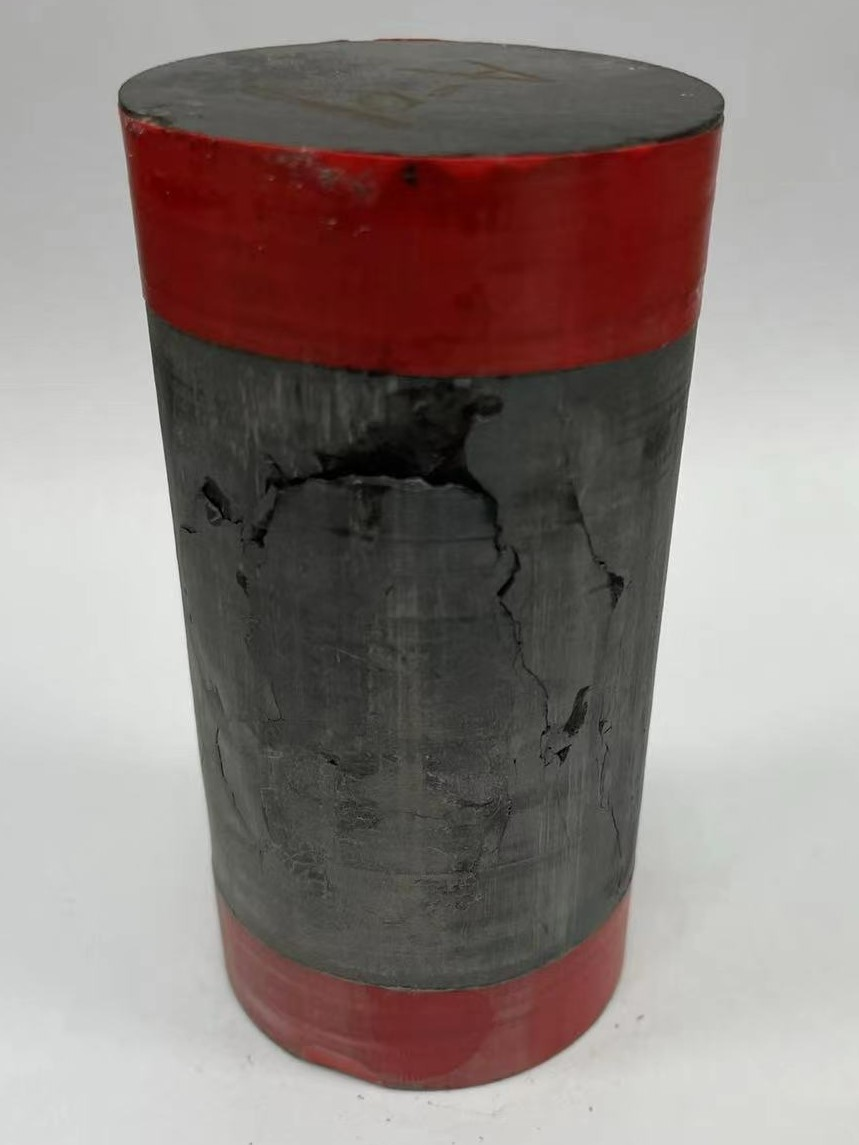
\includegraphics[width=0.9\textwidth]{img/chap2/A-01.jpg}
        \end{minipage}
    }
    \subfigure[B-02]
    {
        \begin{minipage}{7cm}
            \centering
            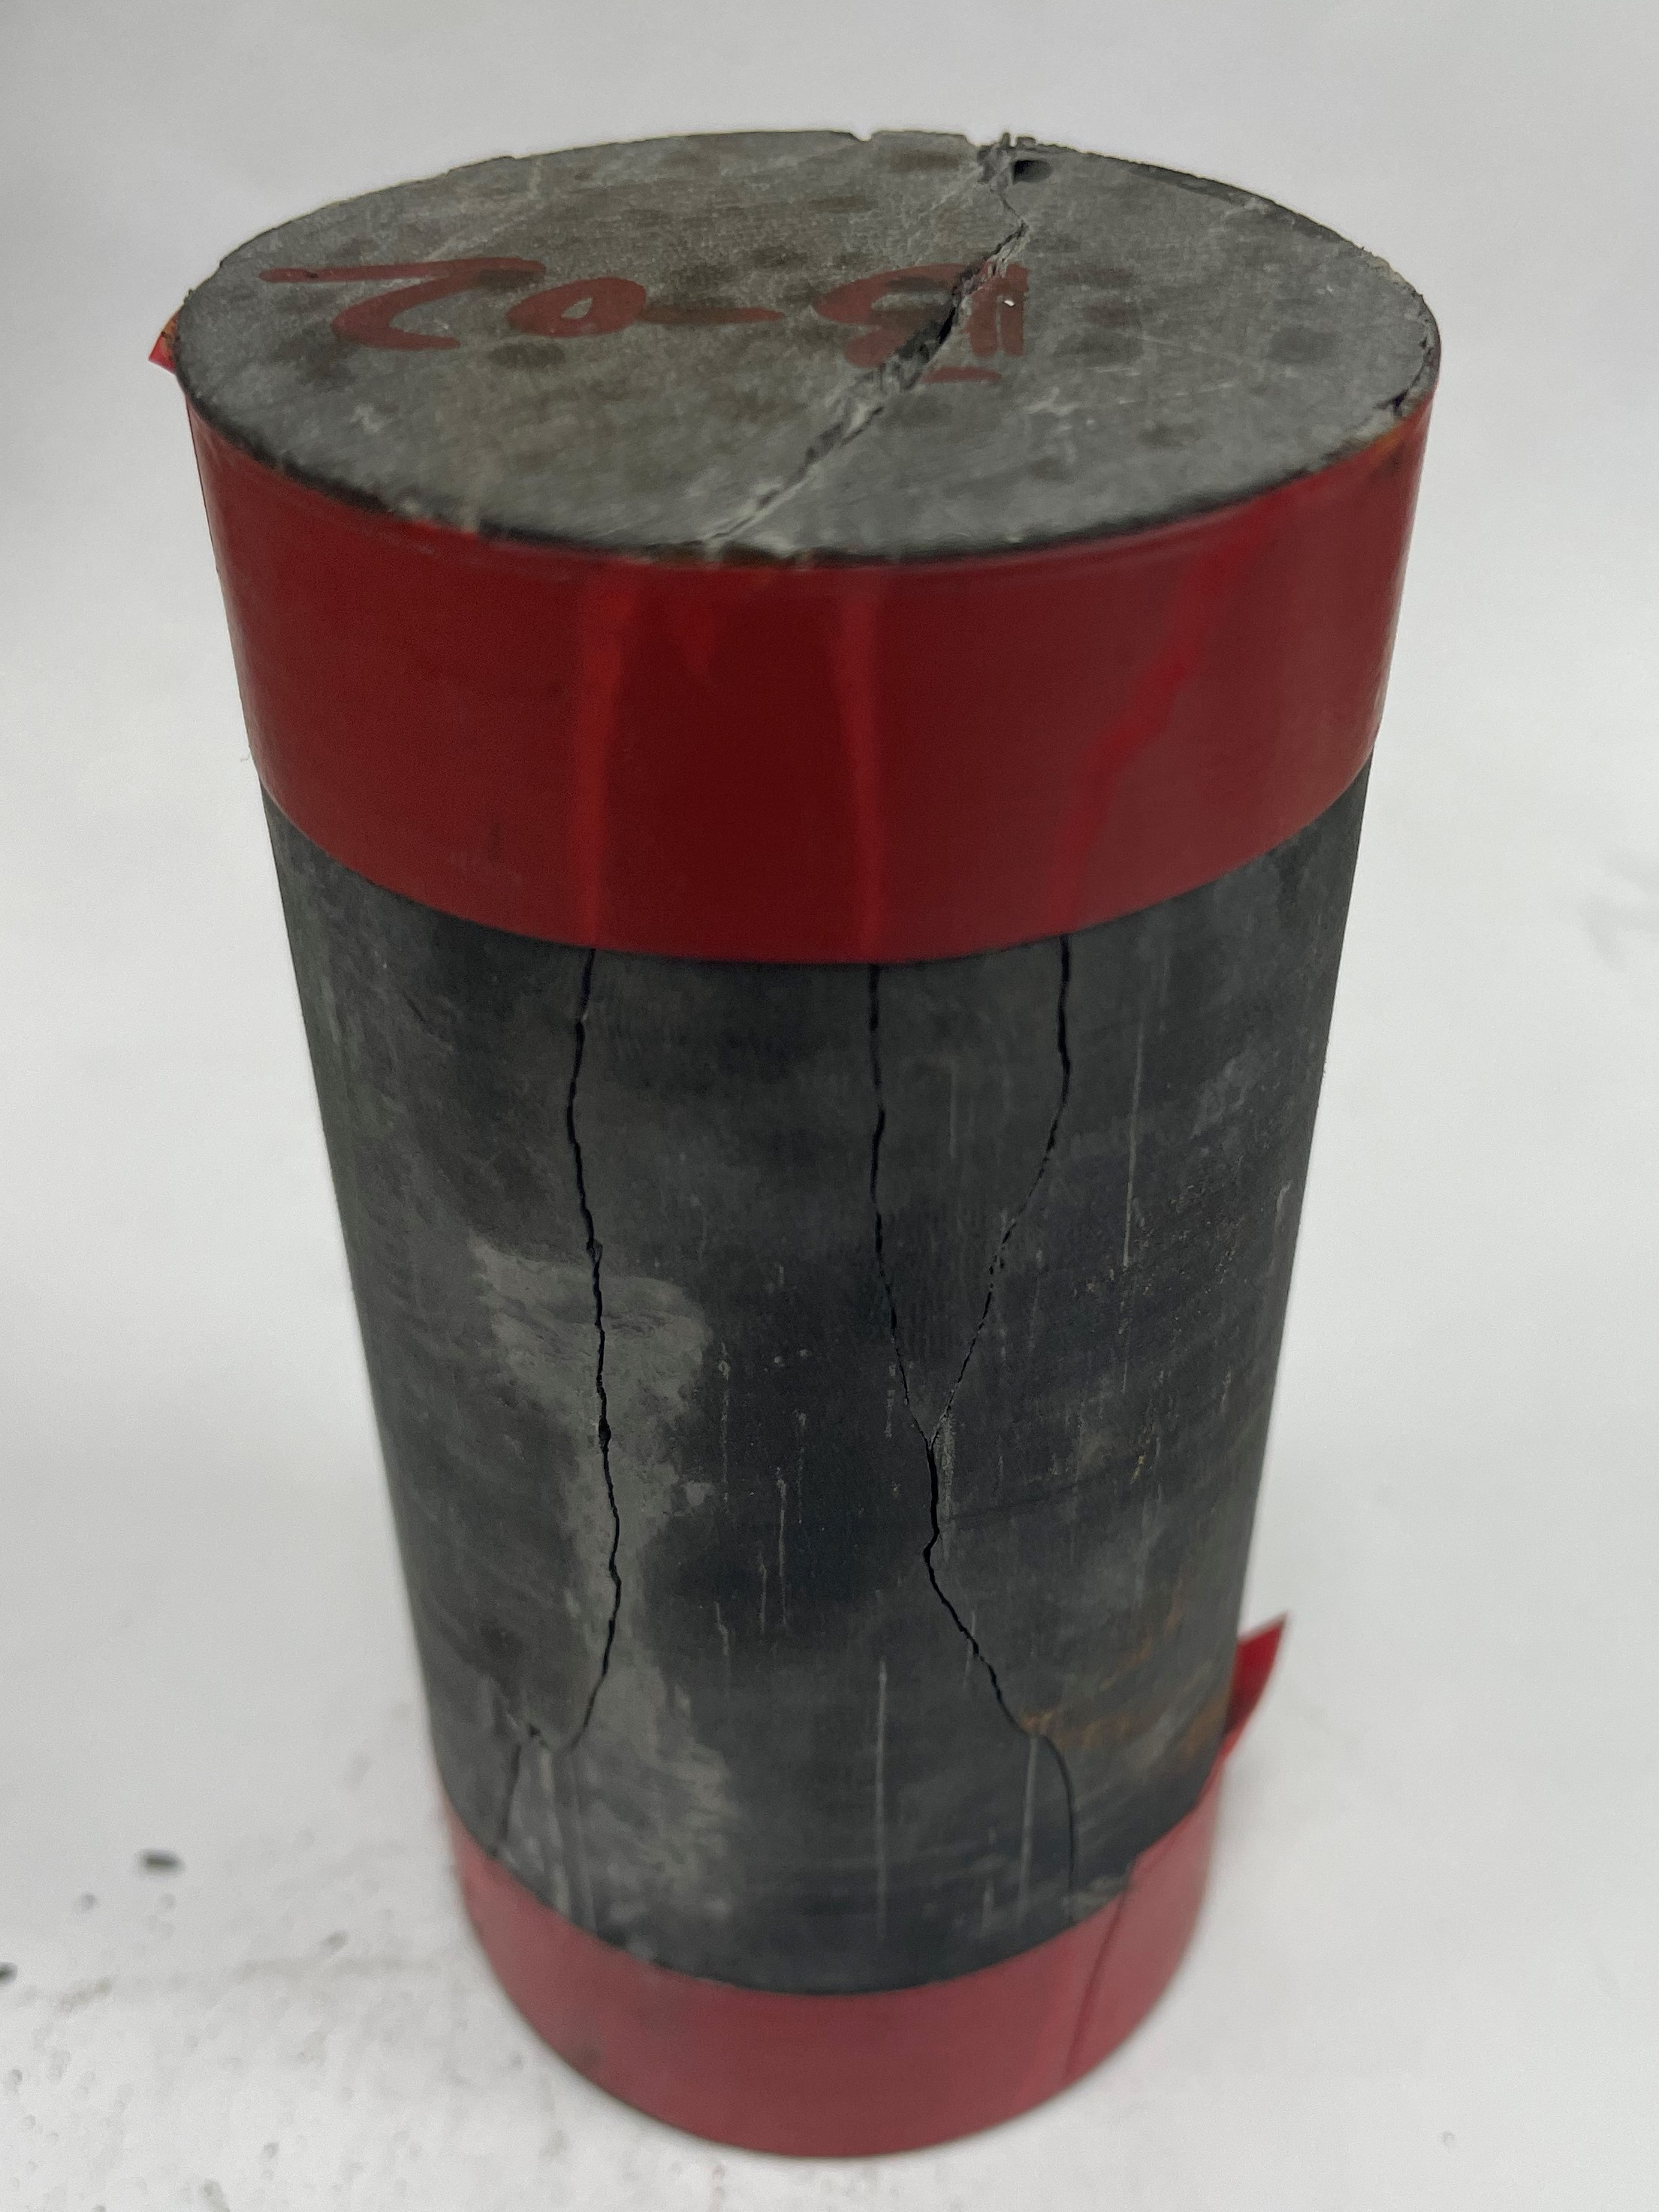
\includegraphics[width=0.9\textwidth]{img/chap2/B-02.jpg}
        \end{minipage}
    }
    \caption{试验步骤}
    \label{fig:2-4}
\end{figure}

由图中可以看出,砂质泥岩在三轴压缩破坏之后并没有表现出如硬岩般的破碎特
征,仍然保持较为完整的圆柱体形状。单轴压缩的试样,如A-01,其整体表现出的破坏形式为张拉破坏,局部出现裂缝,而三轴压缩下的B-02试样,裂缝贯穿整个试件,主要表现为剪切破坏。


\subsection{试样应力-应变曲线分析}
泥岩试样在不同围压下进行常规三轴压缩试验所得的应力-应变曲线如图~\ref{fig:2-4}所示。由图中的($\sigma_1$-$\sigma_3$)\textasciitilde $\varepsilon_1$关系曲线可以看
出,在试验初期阶段,试样在较低的轴压和围压的共同作用下已经完成了压密过程,处于弹性状态。通过图中曲线可以很明显地看出单轴压缩条件下的试样,最终的抗压强度远小于三轴压缩下的试样,单轴压缩条件下,试样在峰值强度附近已经出现了明显的屈服平台,表现出明显的脆性和应变软化特征。三轴压缩条件下,随着围压的增大,曲线弹性阶段的斜率也逐渐增大,极限承载能力和弹性模量也逐渐增大。

\begin{figure}[ht!]
    \centering
    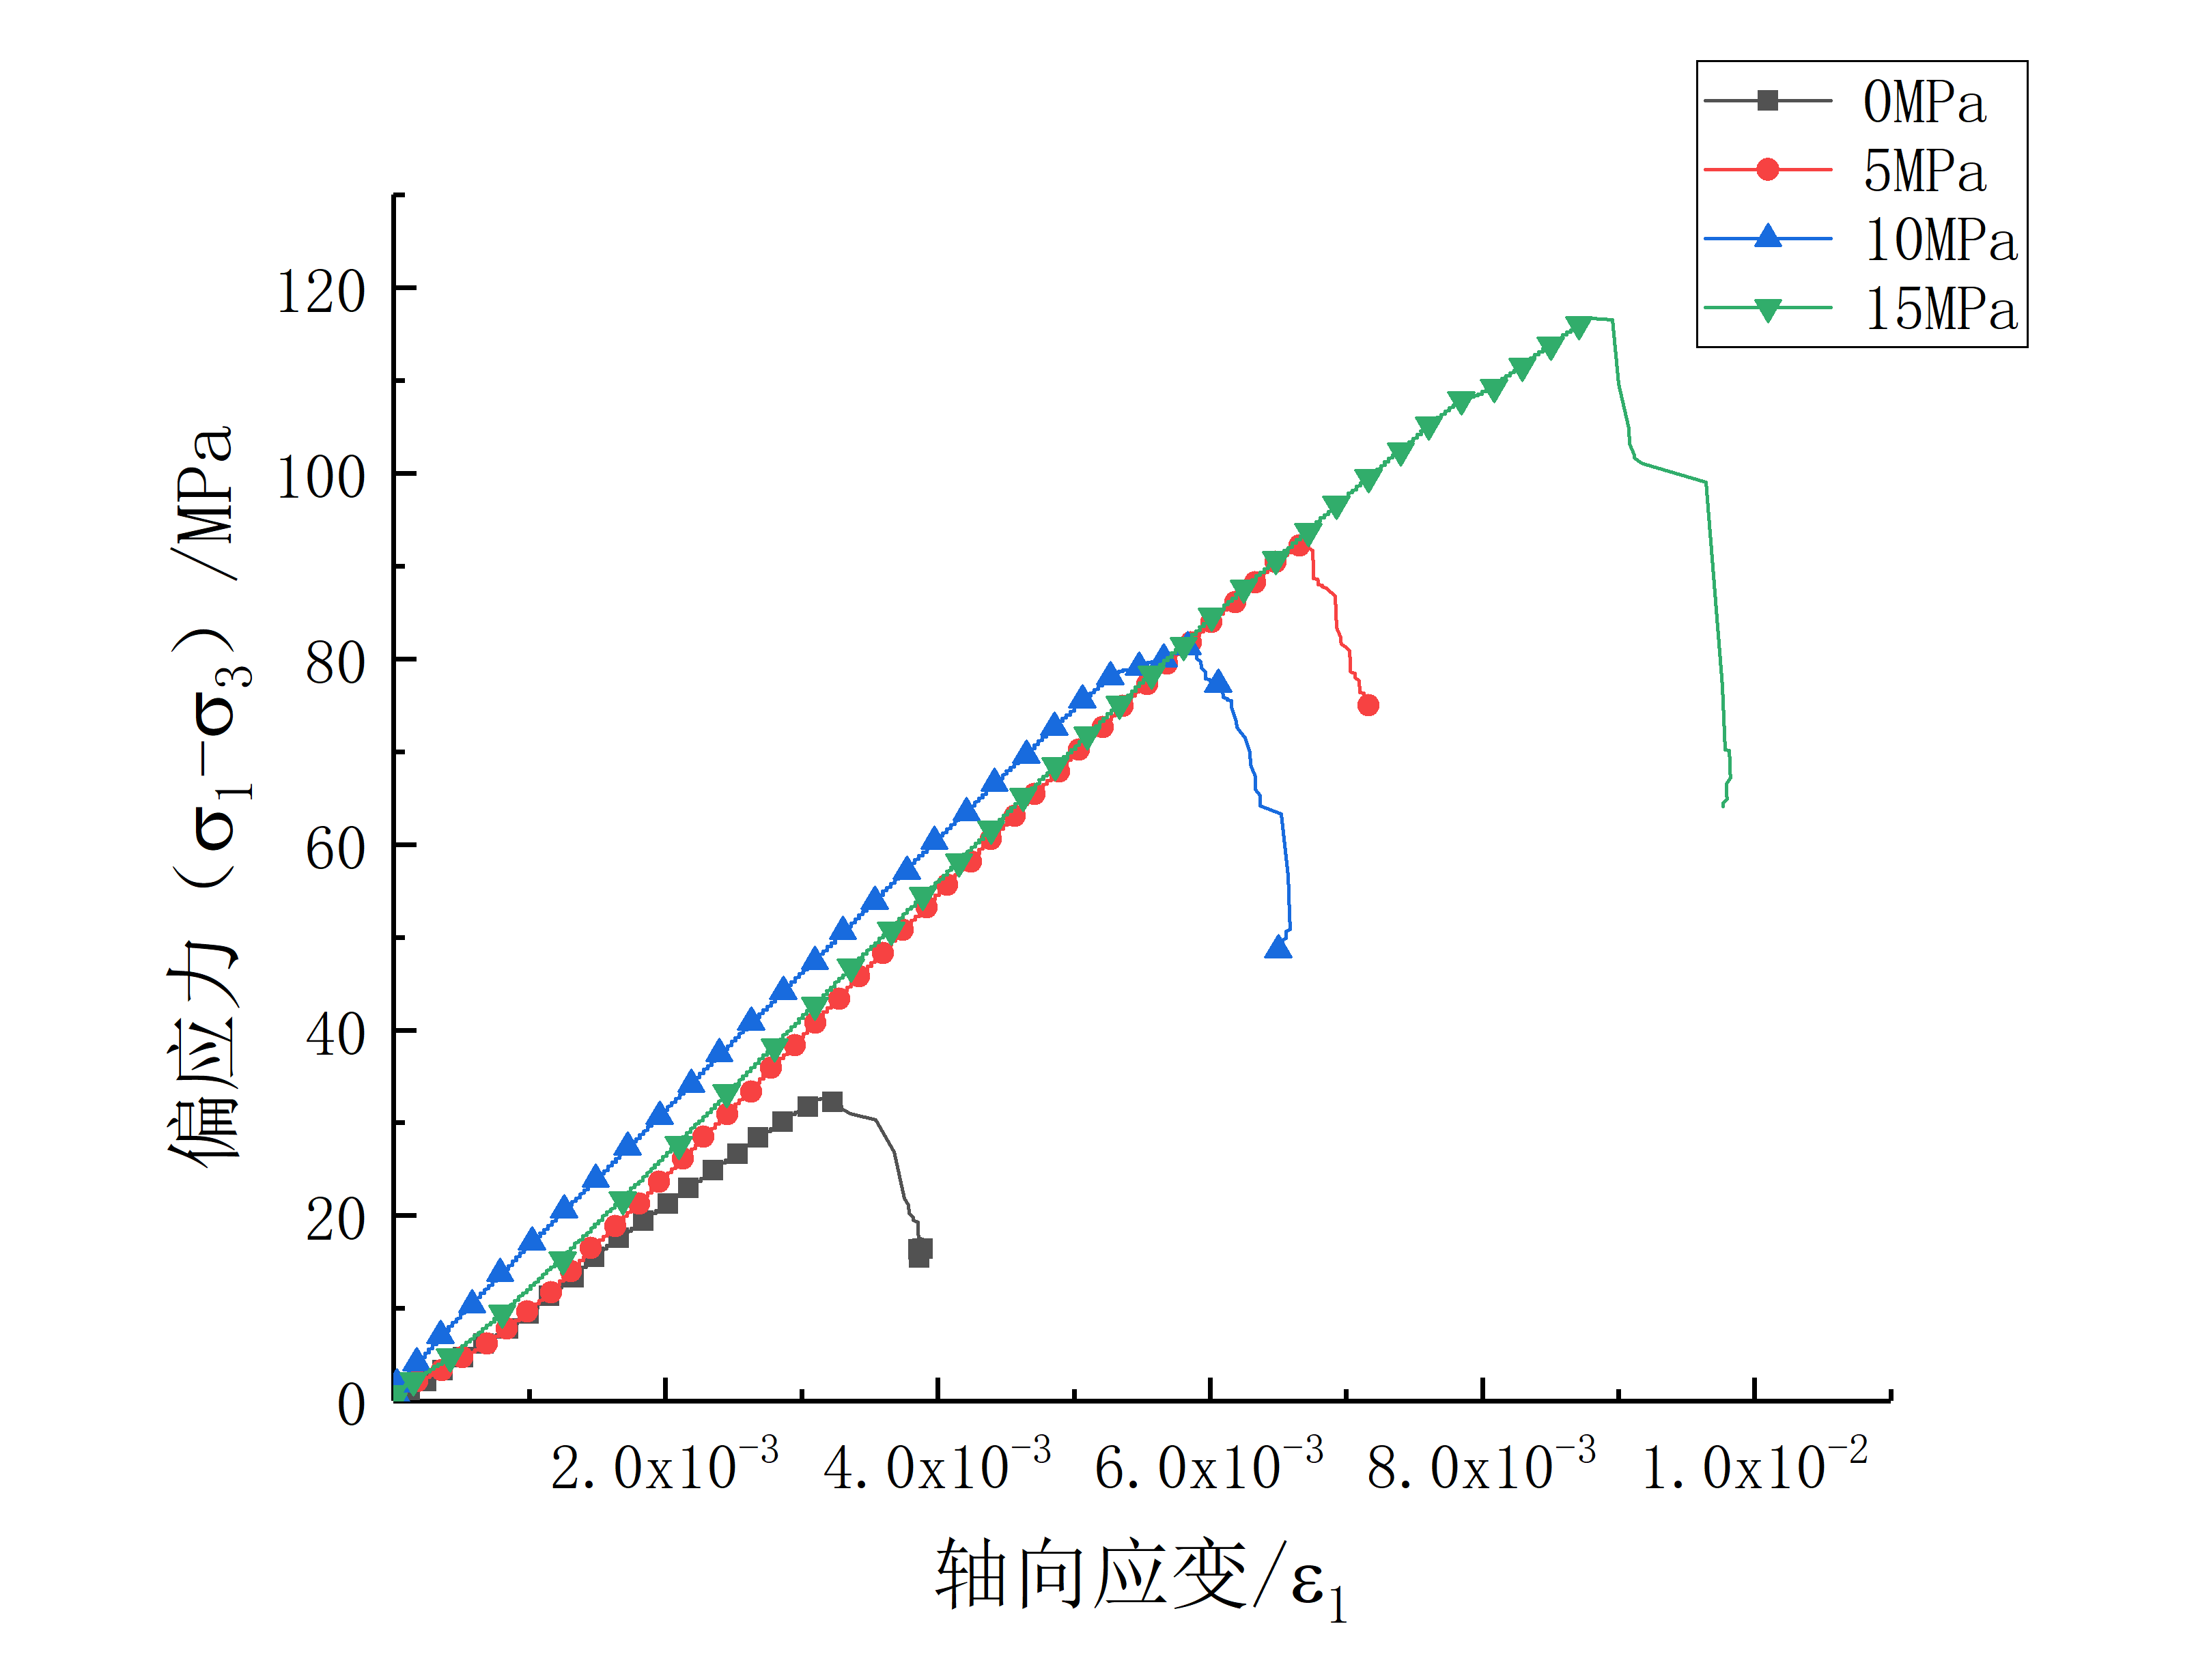
\includegraphics[width=0.7\textwidth]{img/chap2/2-4.png}
    \caption{泥岩三轴压缩应力-应变曲线}
    \label{fig:2-5}
\end{figure}

结合图2.4进行分析,整个试验过程的应力-应变曲线大致分为三个阶段:

(1)弹性变形阶段:该阶段应力一应变曲线呈直线关系,不仅意味着应变随应力成比例的增加,还表现为弹性变形的可恢复。曲线图中弹性阶段直线部分的斜率即为该岩石试样的弹性模量;

(2)微裂隙发展阶段:该阶段岩体中微裂隙开始产生、扩展、累积,新出现的裂纹随着应力的增大而不断发展,岩石产生不可逆变形,即产生相当部分的塑性变形,该阶段的上界称为屈服极限。当微裂隙稳定发展到一定程度后,会进入不稳定发展的状态,在这个过程中,试样薄弱处出现破坏,应力重分布后转嫁至次薄弱部位,次薄弱部位继续破坏直至试样完全破坏。在图~\ref{fig:2-4}中,该阶段表现不太明显,不过图中\SI{10}{MPa}和\SI{15}{MPa}的曲线在弹性阶段和曲线下降段之间可以看到一段与线性变化的直线不同的曲线段。本阶段的上界应力称为峰值强度;

(3)破裂后阶段:岩块达峰值后,内部结构破坏,但整体状态仍旧基本保持,岩样受力主要依靠裂隙面的摩擦力承担。到本阶段,裂隙快速发展,交叉且相互联合形成宏观断裂面试件承载力随变形增大迅速下降,但并不降到零,说明破裂的岩石仍有一定的承载力。

根据试验得到岩石的抗压强度,计算岩石弹性模量,计算公式如下:
\begin{equation}
    E=\frac{\sigma_b-\sigma_a}{\varepsilon_b-\varepsilon_a}
\end{equation}
\begin{shizhong}
     \item $\sigma_a$——应力—应变曲线弹性阶段应力峰值的30\%
     \item $\sigma_b$——应力—应变曲线弹性阶段应力峰值的50\%
     \item $\varepsilon_a$——应力为$\sigma_a$时的轴向应变值     
     \item $\varepsilon_b$——应力为$\sigma_b$时的轴向应变值
\end{shizhong}
 
经整理得岩石单轴压缩试验结果如表\ref{tab:泥岩单、三轴试验结果}所示。单轴压缩条件下,泥岩的峰值强度均值为\SI{28.13}{MPa},弹性模量为\SI{12.927}{GPa};而在三轴压缩的条件下,该种泥岩试样的抗压峰值强度大大提升,其均值约为\SI{96.80}{MPa},弹性模量为\SI{14.873}{GPa},由此可见围压对泥岩的强度和刚度都有较大影响。
\begin{table}[ht!]\small
    \centering
    \begin{tabular}{p{3cm}<{\centering} p{3cm}<{\centering} p{3cm}<{\centering} p{3cm}<{\centering}}
        \toprule
        试样编号  & 峰值强度/MPa  &  峰值应变   &  弹性模量/GPa\\
        \midrule
        A-01        & 32.75  &   0.0032  &  12.873   \\ 
        A-02        & 26.03 &   0.0027  &  13.906   \\ 
        A-03        & 25.61  &   0.0028  &  12.003  \\ 
        \midrule
        B-01        & 92.35  &   0.0067  &  15.330   \\ 
        B-02        & 81.32 &   0.0058 &  14.626   \\ 
        B-03        & 116.74 &   0.0088  &  14.679 \\ 
        \bottomrule
    \end{tabular}
    \caption{泥岩单、三轴试验结果}
    \label{tab:泥岩单、三轴试验结果}
\end{table}

    
在本次试验获得的曲线中,有两个阶段受试验环境的影响,在图中没有明显表示:一是在弹性阶段开始前,试样受到轴压和围压共同作用所导致的空隙压密阶段,在此阶段,岩石中原有的空隙在较低的轴压和围压共同作用下逐渐闭合,岩石被压密,形成初始非线性变形;二是在试件破坏后达到的塑性流动阶段,随着塑性变形的持续发展,最终强度不再降低,这是由于所用的刚性三轴压缩仪所设定的试样破坏即停止试验,没有继续对破坏的试件施加轴向应力,所以没有塑性流动阶段的试验记录。


\section{泥岩单轴流变试验}\label{section:泥岩单轴流变试验}
\subsection{流变试验过程}
常规室内岩石蠕变试验的加载方式一般有三种,分别是分别加载、分级加载以及分级加卸载。分别加载法是用同种岩样制成一组试样,在相同的试验条件下对每个试样施加不
同的恒定荷载,观察同一组试样在不同加载应力下的流变过程。该方法能够使试样避免受到加载状态和加载历史的影响,蠕变曲线可以不经处理直接应用,实验结果理想可靠。然而,每个试样性质很难完全一致导致试验结果离散性较大,并且所需试验设备数量较多会使得试验成本过高,一般实验室难以满足。

分级加载法是在同一试样上逐级施加荷载,在一级荷载施加后,岩样经历给定的
的蠕变趋于稳定或达到预期时,再施加下一级荷载。该方法可在同一试样上获得更多的试验资料,结果离散性较小,可以减少试验操作过程中产生的误差。其缺点是试样在各级荷载下的变形相互交叉影响,该方法所得蠕变曲线为阶梯状,直接应用较少,需对蠕变曲线经过处理后才方便应用。

分级加卸载是指在一个试样上施加一定荷载,在荷载作用下变形基本稳定后卸除荷载,当滞后弹性变形恢复稳定(不增长),再在同一试样上进行下一级荷载的循环,直至试样加载到预设的应力等级或试样破坏,它吸收了分级加载法的优点,又在理论上避免了各级荷载下的变形相互影响。但在实际过程中,频繁的加卸载会导致岩石的性质发生改变。

通过对规格为直径\SI{50}{mm},高为\SI{100}{mm}的标准圆柱体的5个泥岩试样进行单轴流变试验,观察在常温下,岩石流变破坏所需的时间。
将试样标号为$C-01$、$C-02$、$C-03$、$C-04$、$C-05$,根据岩石单轴压缩试验确定岩石变形破坏最基本的力学特
性及参数,合理地选取加载应力水平进行流变试验,具体工况如表~\ref{tab:泥岩单轴流变试验工况表}所示:

\begin{table}[ht!]\small
    \centering
    \begin{tabular}{p{3cm}<{\centering} p{3cm}<{\centering} p{3cm}<{\centering} p{3cm}<{\centering}}
        \toprule
        试样编号  & 围压(MPa)  &  加载强度(MPa)   &  加载时间(h)\\
        \midrule
        C-01        & 0  &   26.3  &     \\ 
        C-02        & 0  &   24.8  &     \\ 
        C-03        & 0  &   23.4  &     加载至试样破坏\\
        C-04        & 0  &   22.0  &     \\
        C-05        & 0  &   20.5  &     \\
        \bottomrule
    \end{tabular}
    \caption{泥岩单轴流变试验工况表}
    \label{tab:泥岩单轴流变试验工况表}
\end{table}




由单轴压缩试验得岩石的强度,并以此为依据确定岩石单轴蠕变试验的加载等级。
在蠕变试验中我们所采用的仪器与上一小节三轴压缩试验使用的仪器为同一台,因此不再多做介绍。试验步骤依据~\ref{section:试验过程}节的基本方案对进行,具体实验过程如下所述:

(1)从试样选取与编号、试样安装到充油施加围压(单轴蠕变试验无须施加围压)这三步与2.2.1节中进行常规三轴压缩试验的前三步操作相同。

(2)在围压施加完成后,将试样与三轴伺服仪轴压压头进行接触,可手动操作向轴压压力室加油,待轴向应变变化说明已经接触,且接触后要卸载此时的偏应力值到零,最后加满轴压泵。

(3)而与三轴压缩试验不同的是,在蠕变实验中,我们采用应力加载方式,加载速度为\SI{3}{MPa/min}。由于采用的时分级加载的方式,根据试验前算得每一级偏应力,当轴压施加到预计值时,需要保持此时的偏应力一段时间,具体时间根据工况表中的预计加载时间以及试样实验时的实际情况确定,待达到预定加载时间后,再施加下一级应力。若试样在某一级加载中损坏,便结束试验并取出损坏的试样。


\subsection{流变特征分析}
研究表明,岩石除了在加载瞬间产生的瞬时变形,随后会发生缓慢且持续的蠕变变形,基于岩石的流变特性,岩石的流变曲线大致上如图~\ref{fig:2-8}所示。岩石蠕变过程一般分为三个阶段,分别是初始变阶段、稳定蠕变阶段和加速蠕变阶段的应变。在初始蠕变阶段,应变随时间增大,但应变增长的速率逐渐减小,因此该阶段也叫减速蠕变阶段;第二阶段是稳定蠕变阶段,岩石的蠕变速率在第一阶段末逐渐减小到一定值后保持不变,在这个阶段蠕变曲线近似直线,应变随时间的增长近似线性增加,蠕变变形最终趋于稳定;第三阶段为加速蠕变阶段,此时蠕变速率随时间迅速增大,岩石变形快速发展直至破坏。

\begin{figure}[ht!]
    \centering
        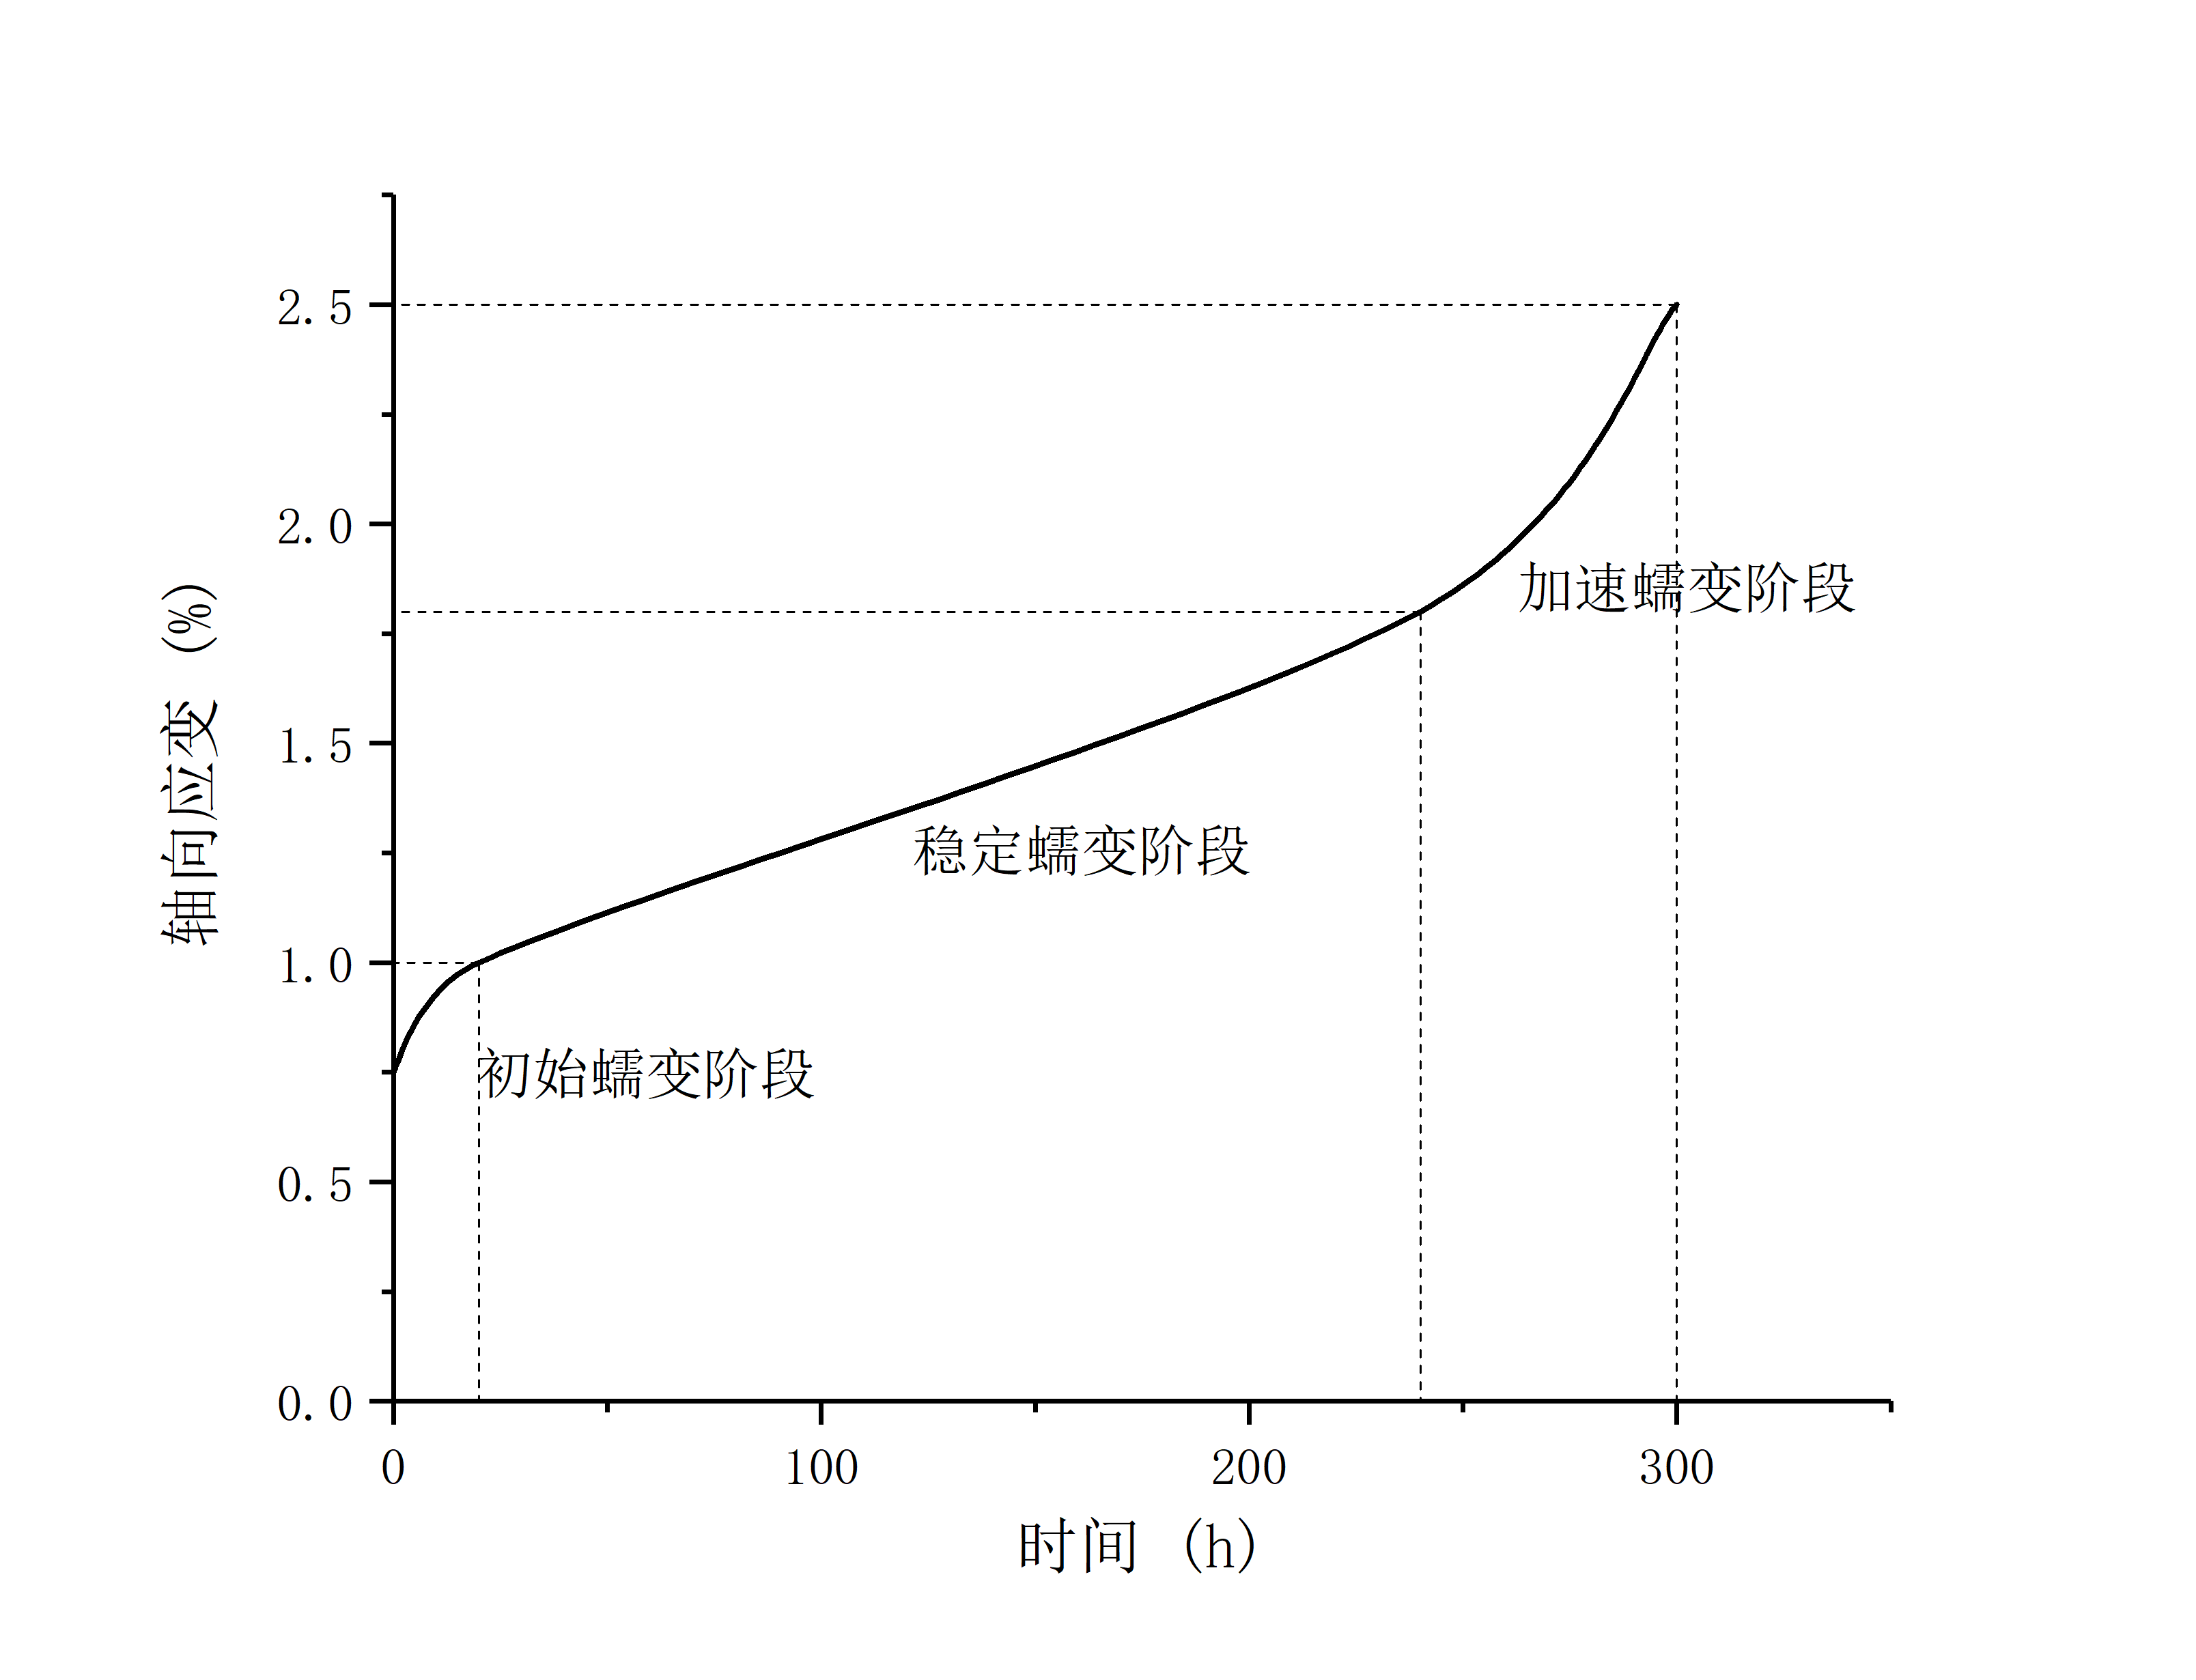
\includegraphics[width=0.7\textwidth]{img/chap2/Creep curve.png}
    \caption{蠕变曲线}
    \label{fig:2-8}
\end{figure}

\subsection{单轴流变曲线分析}

流变试验结束后,我们对收集到的实验数据进行集中处理,由此可以得到各个试样的流变数据曲线,进行分别加载的单轴压缩流变试验所得到曲线如图~\ref{fig:2-9}所示,我们可以发现:

(1)在我们所完成的5个单轴压缩流变试验中,试样在加载的瞬间都会产生瞬时压缩变形。并且根据试验工况表中的加载强度,结合试验数据来看,试样发生的瞬时轴向应变会随着加载强度的增大而增大。例如,在C-01试样中,加载到预定的强度等级后,瞬时应变达到了0.21\%,C-02的瞬时应变则为0.19\%。

(2)除 C-03 外,其余四组试验在产生瞬时变形后,其轴向应变仍会随时间的增长缓慢增加,说明试样进入了蠕变过程,进入蠕变阶段后,变形会随着时间增加,蠕变变形趋于稳定,故在图中看起来近似一条直线。而 C-03 试样在加载到预定应力等级的过程中也产生了瞬时轴向应变,不过从实验数据上看,在达到蠕变阶段不久,施加的偏应力迅速减小,轴向应变突然增大,试样进入加速蠕变阶段,此时试样已经破坏,可以认为在加载过程中岩样已经积累大量损伤,故不作为流变破坏讨论。

(3)从图(a)中可以看出,相比C-02、C-04、C-05,C-01在达到蠕变阶段后,轴向应变依旧有明显的上升。因此,在应力水平较高时,试样蠕变达到稳定后,轴向应变依旧会产生,在经历一定时间后流变变形量呈线性增长,流变变形速率趋于某一不为零的定值。而在较低的应力水平下,试样在达到蠕变后,蠕变速率会减小到接近于0,蠕变应变基本不再产生,这种情况下,整个试验的变形过程就是以试样的瞬时轴向应变和一小段的初始蠕变过程为主。

(4)在流变曲线中,试样在达到稳定流变阶段后,在某些时间节点上,轴向应变会突然上下波动,这是因为试样中存在着初始损伤,试样中的微小裂隙在偏应力作用下不断发展,造成局部破裂形成的,对流变过程产生了一定的影响,不过这种影响并不显著。

\begin{figure}[ht!]
    \centering
    \subfigure[C-01]
    {
        \begin{minipage}{7cm}
            \centering
            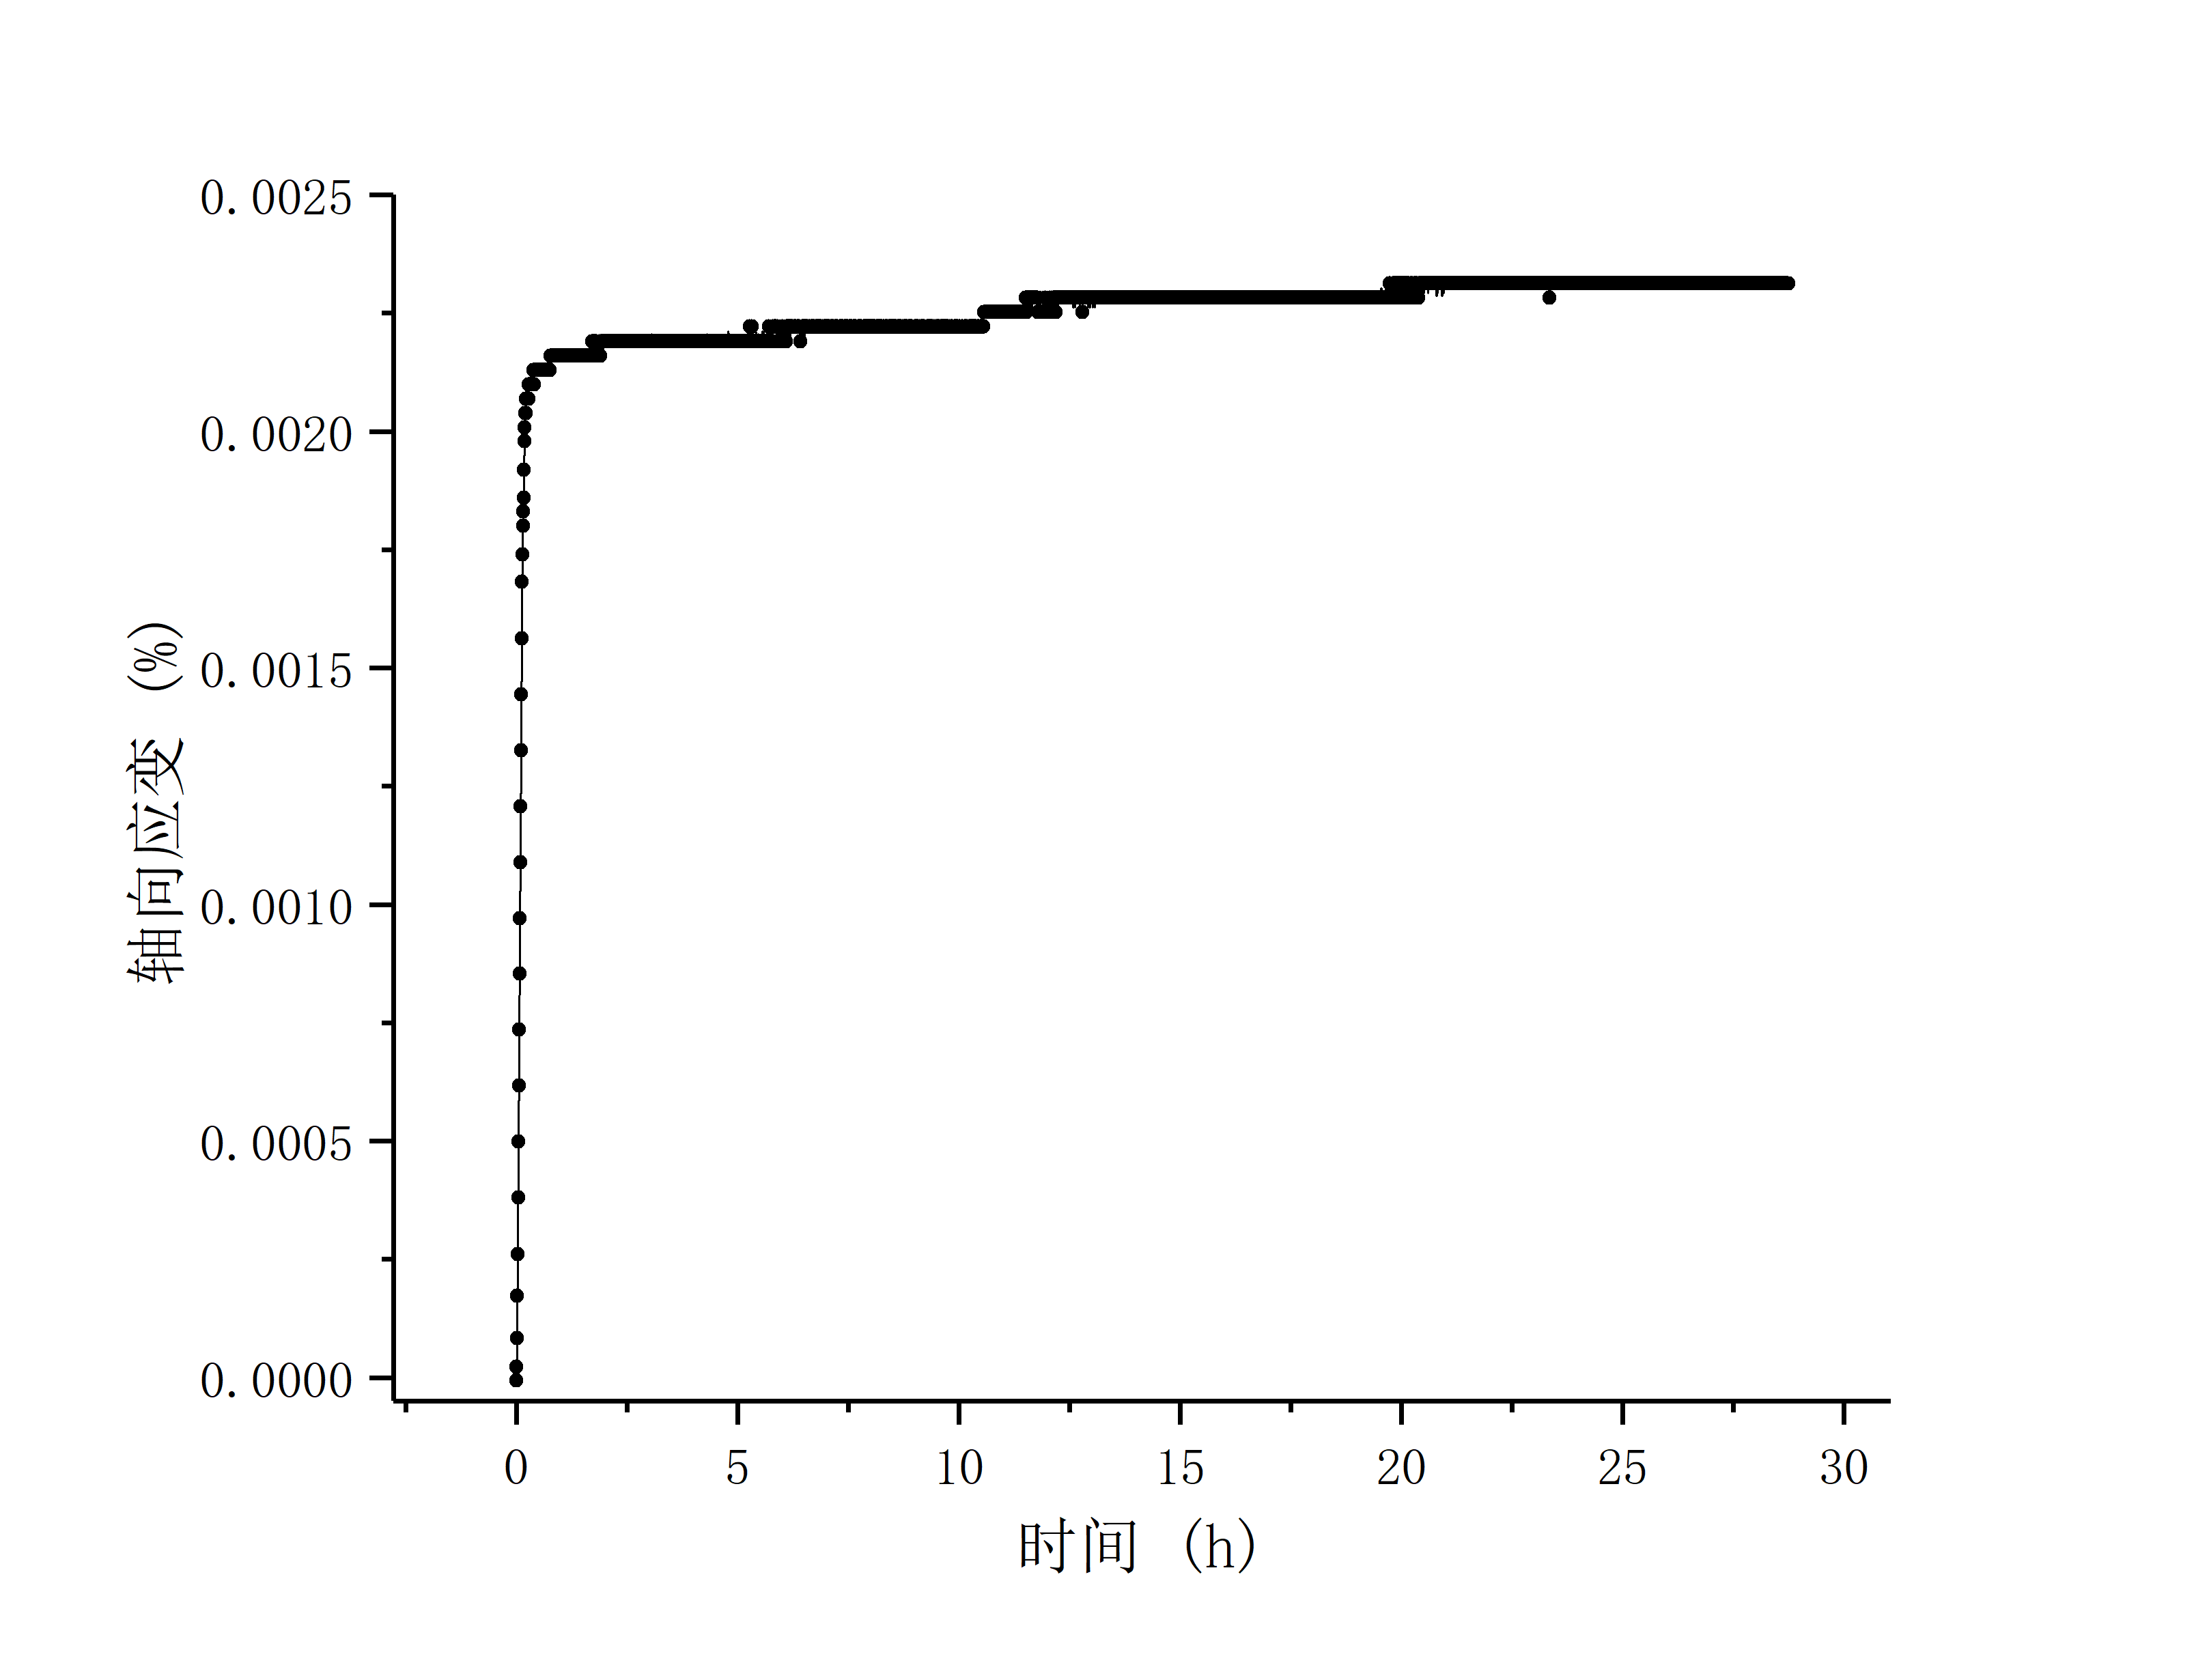
\includegraphics[width=1.1\textwidth]{img/chap2/C-01.png}
        \end{minipage}
    }
    \subfigure[C-02]
    {
        \begin{minipage}{7cm}
            \centering
            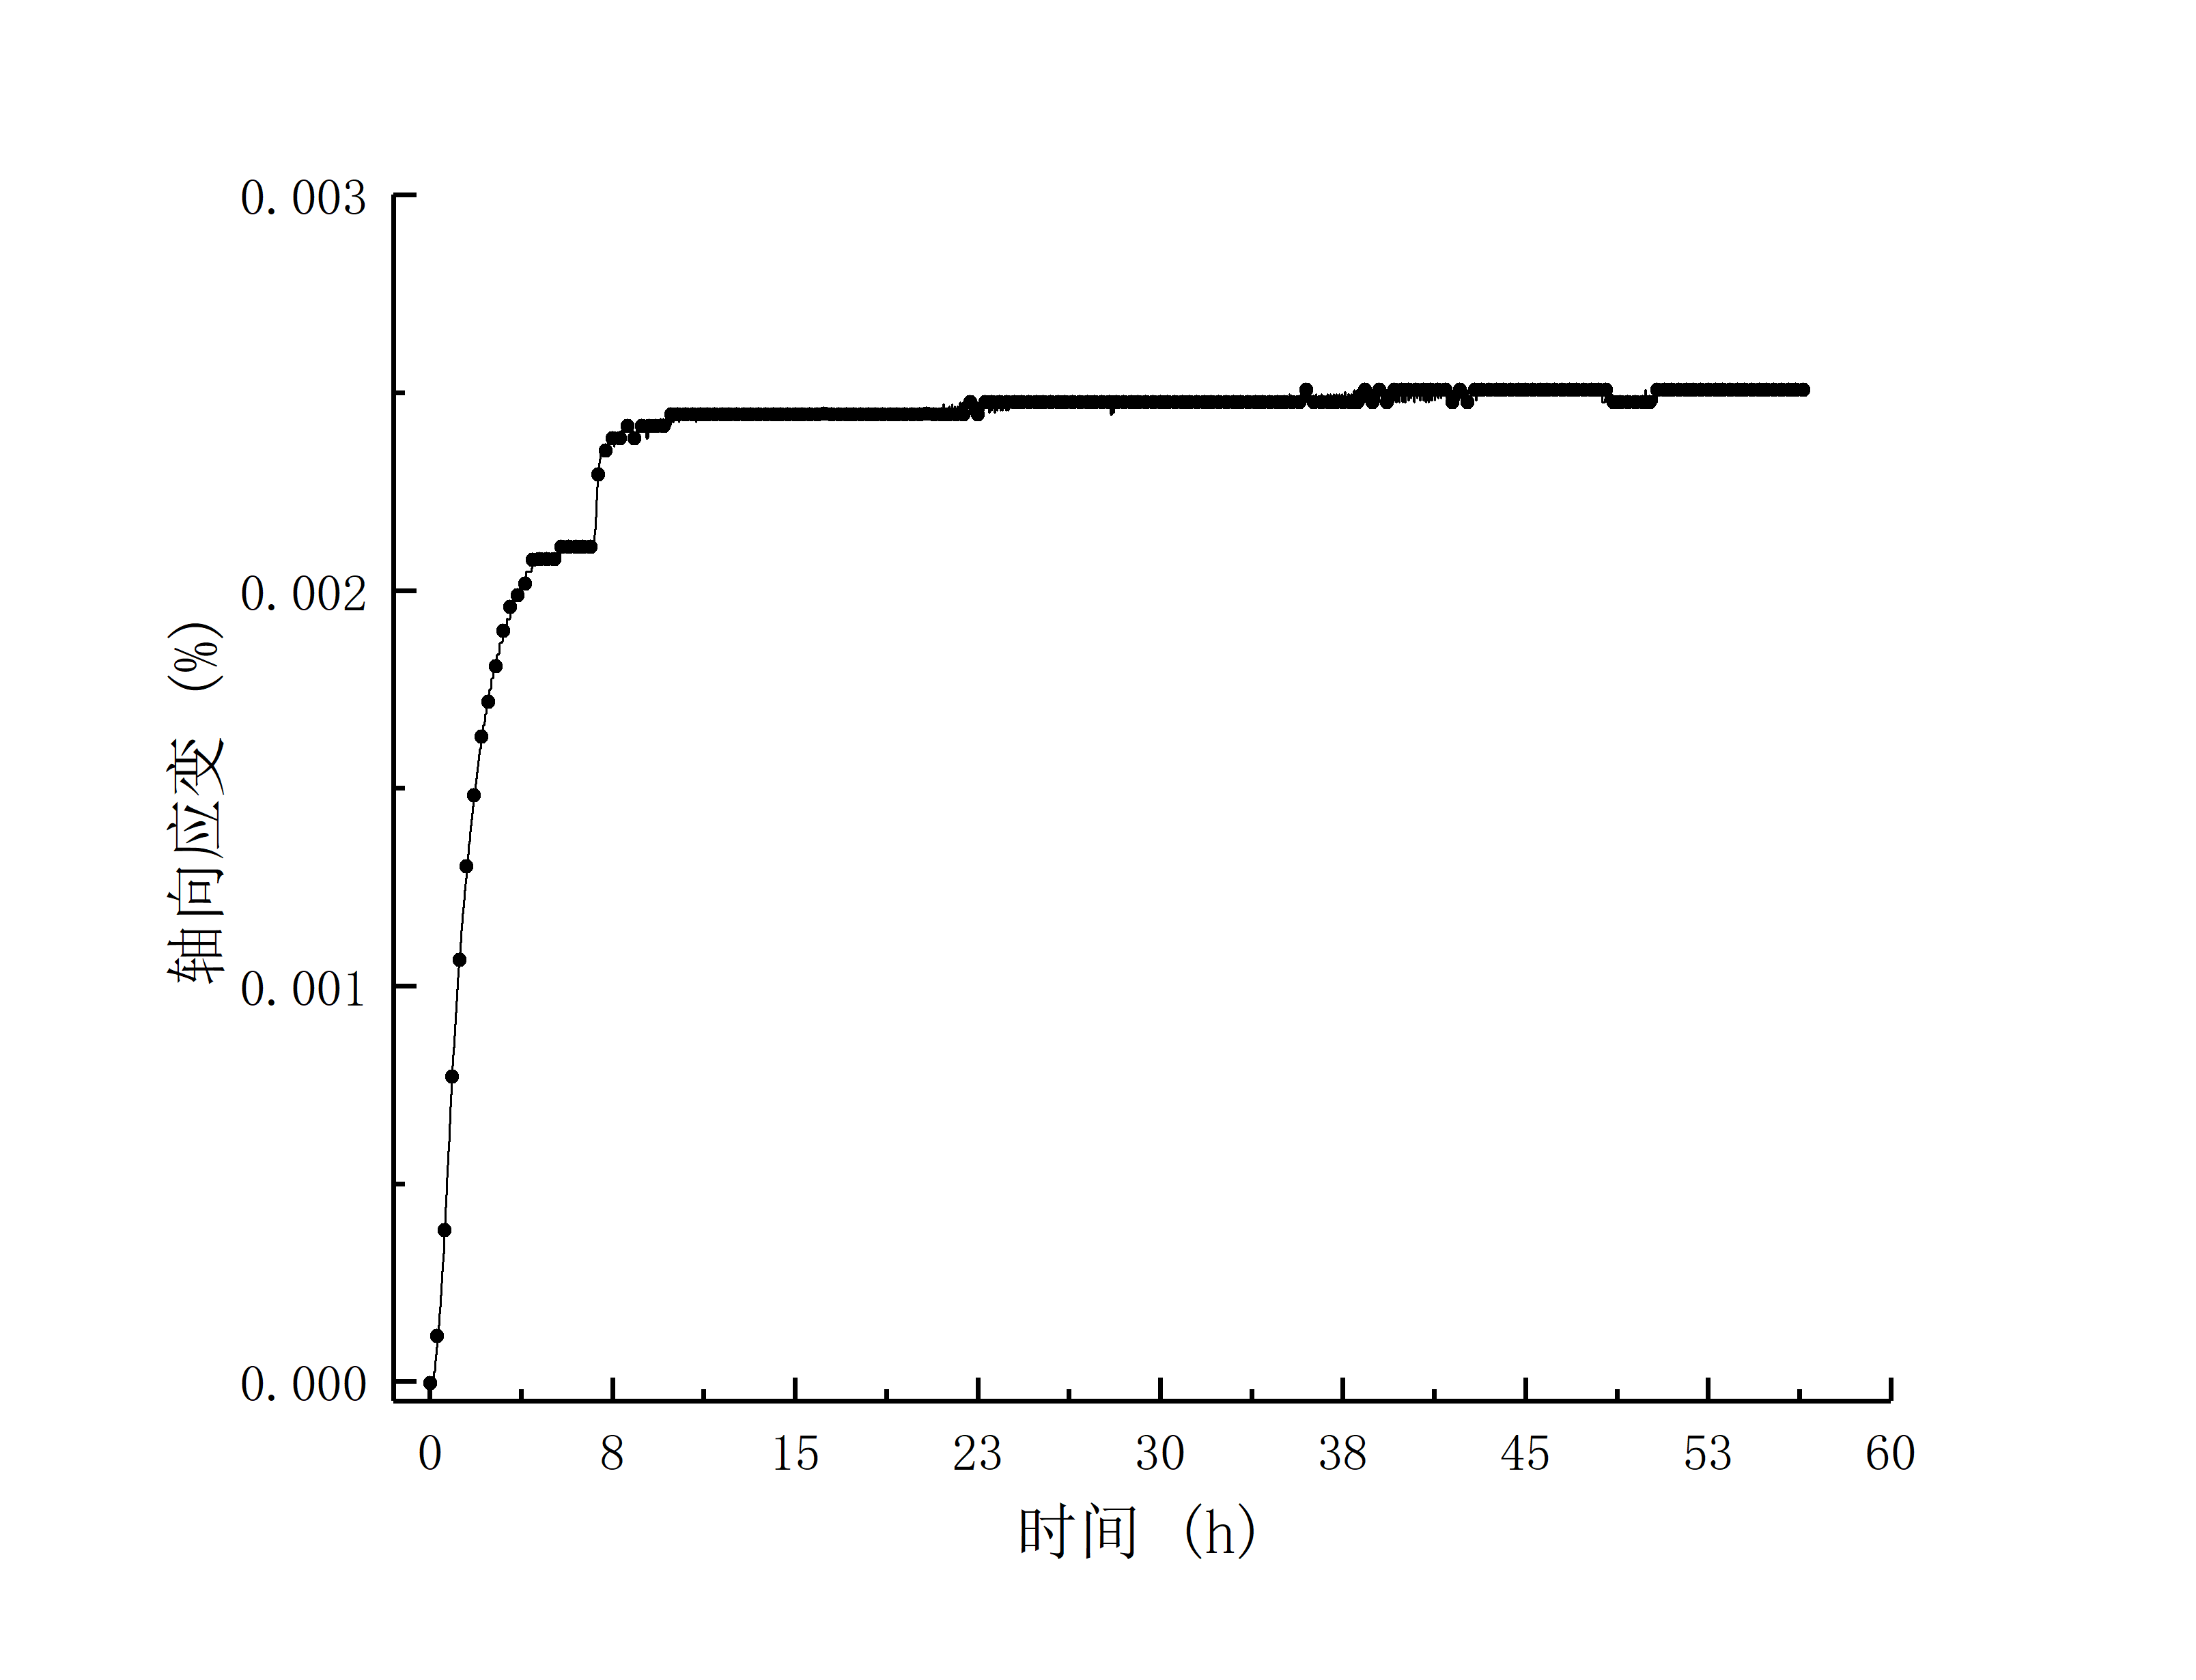
\includegraphics[width=1.1\textwidth]{img/chap2/C-02.png}
        \end{minipage}
    }
	
    \subfigure[C-03]
    {
        \begin{minipage}{7cm}
            \centering
            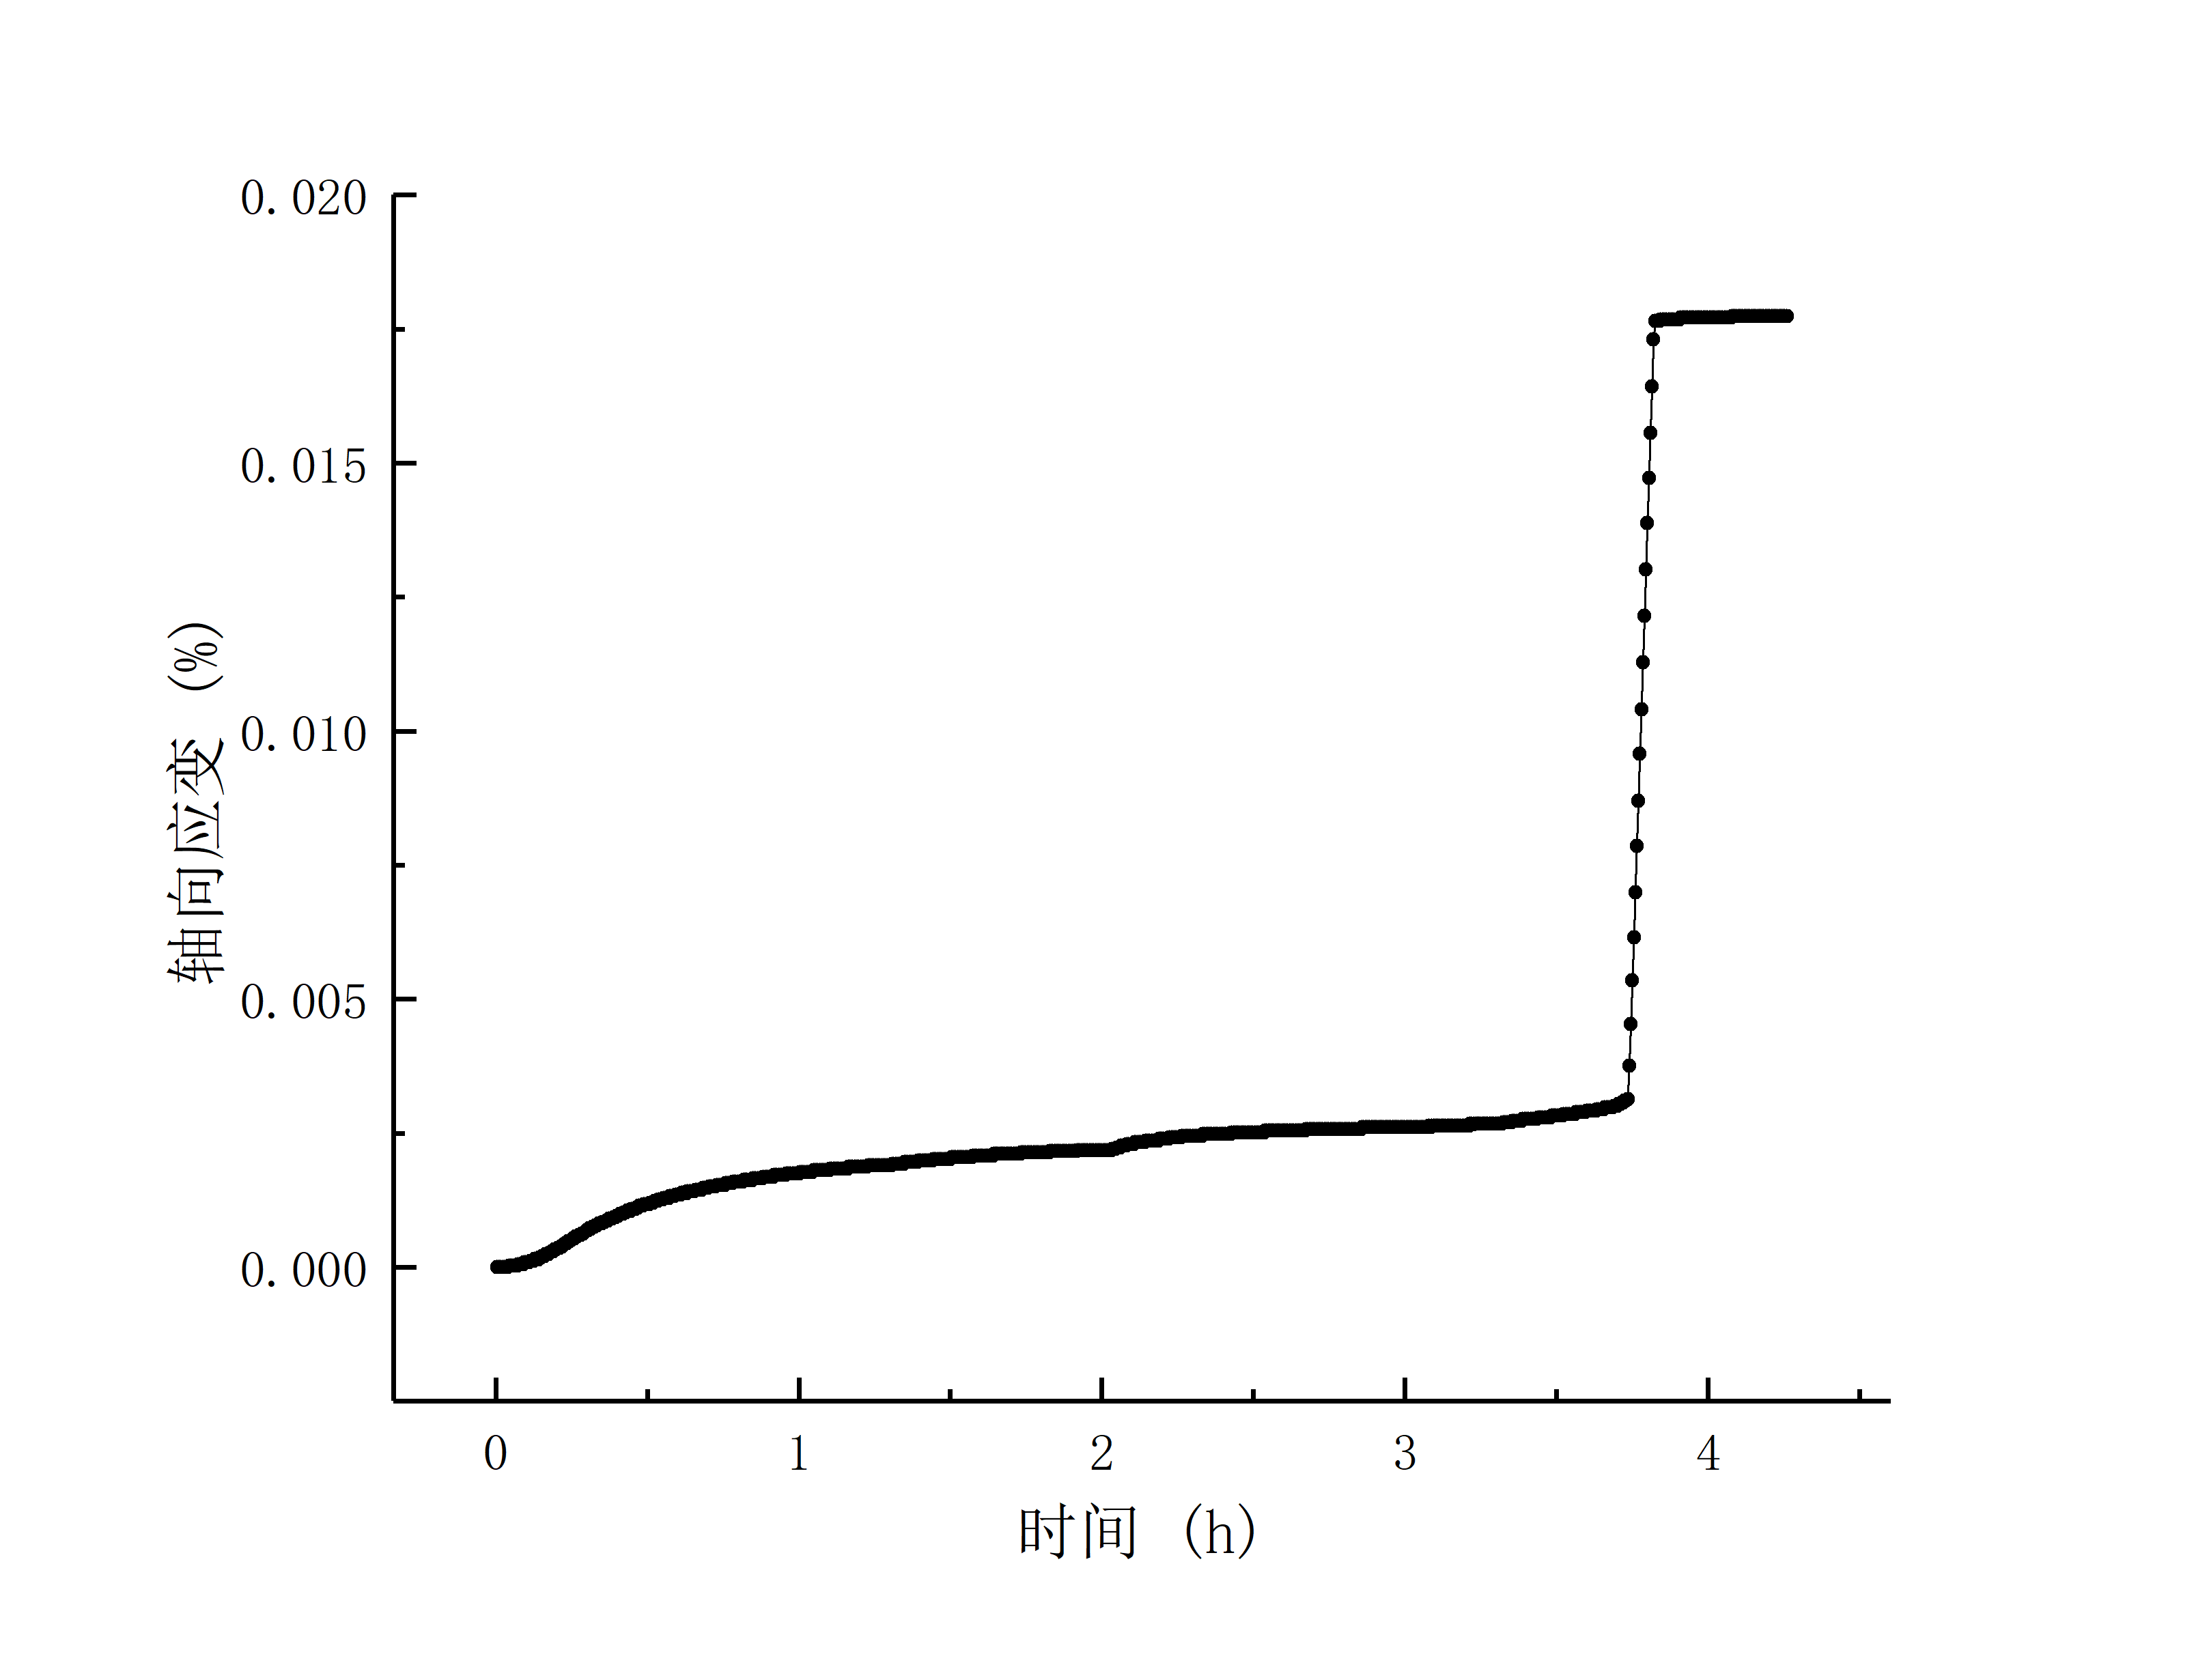
\includegraphics[width=1.1\textwidth]{img/chap2/C-03.png}
        \end{minipage}
    }
    \subfigure[C-04]
    {
        \begin{minipage}{7cm}
            \centering
            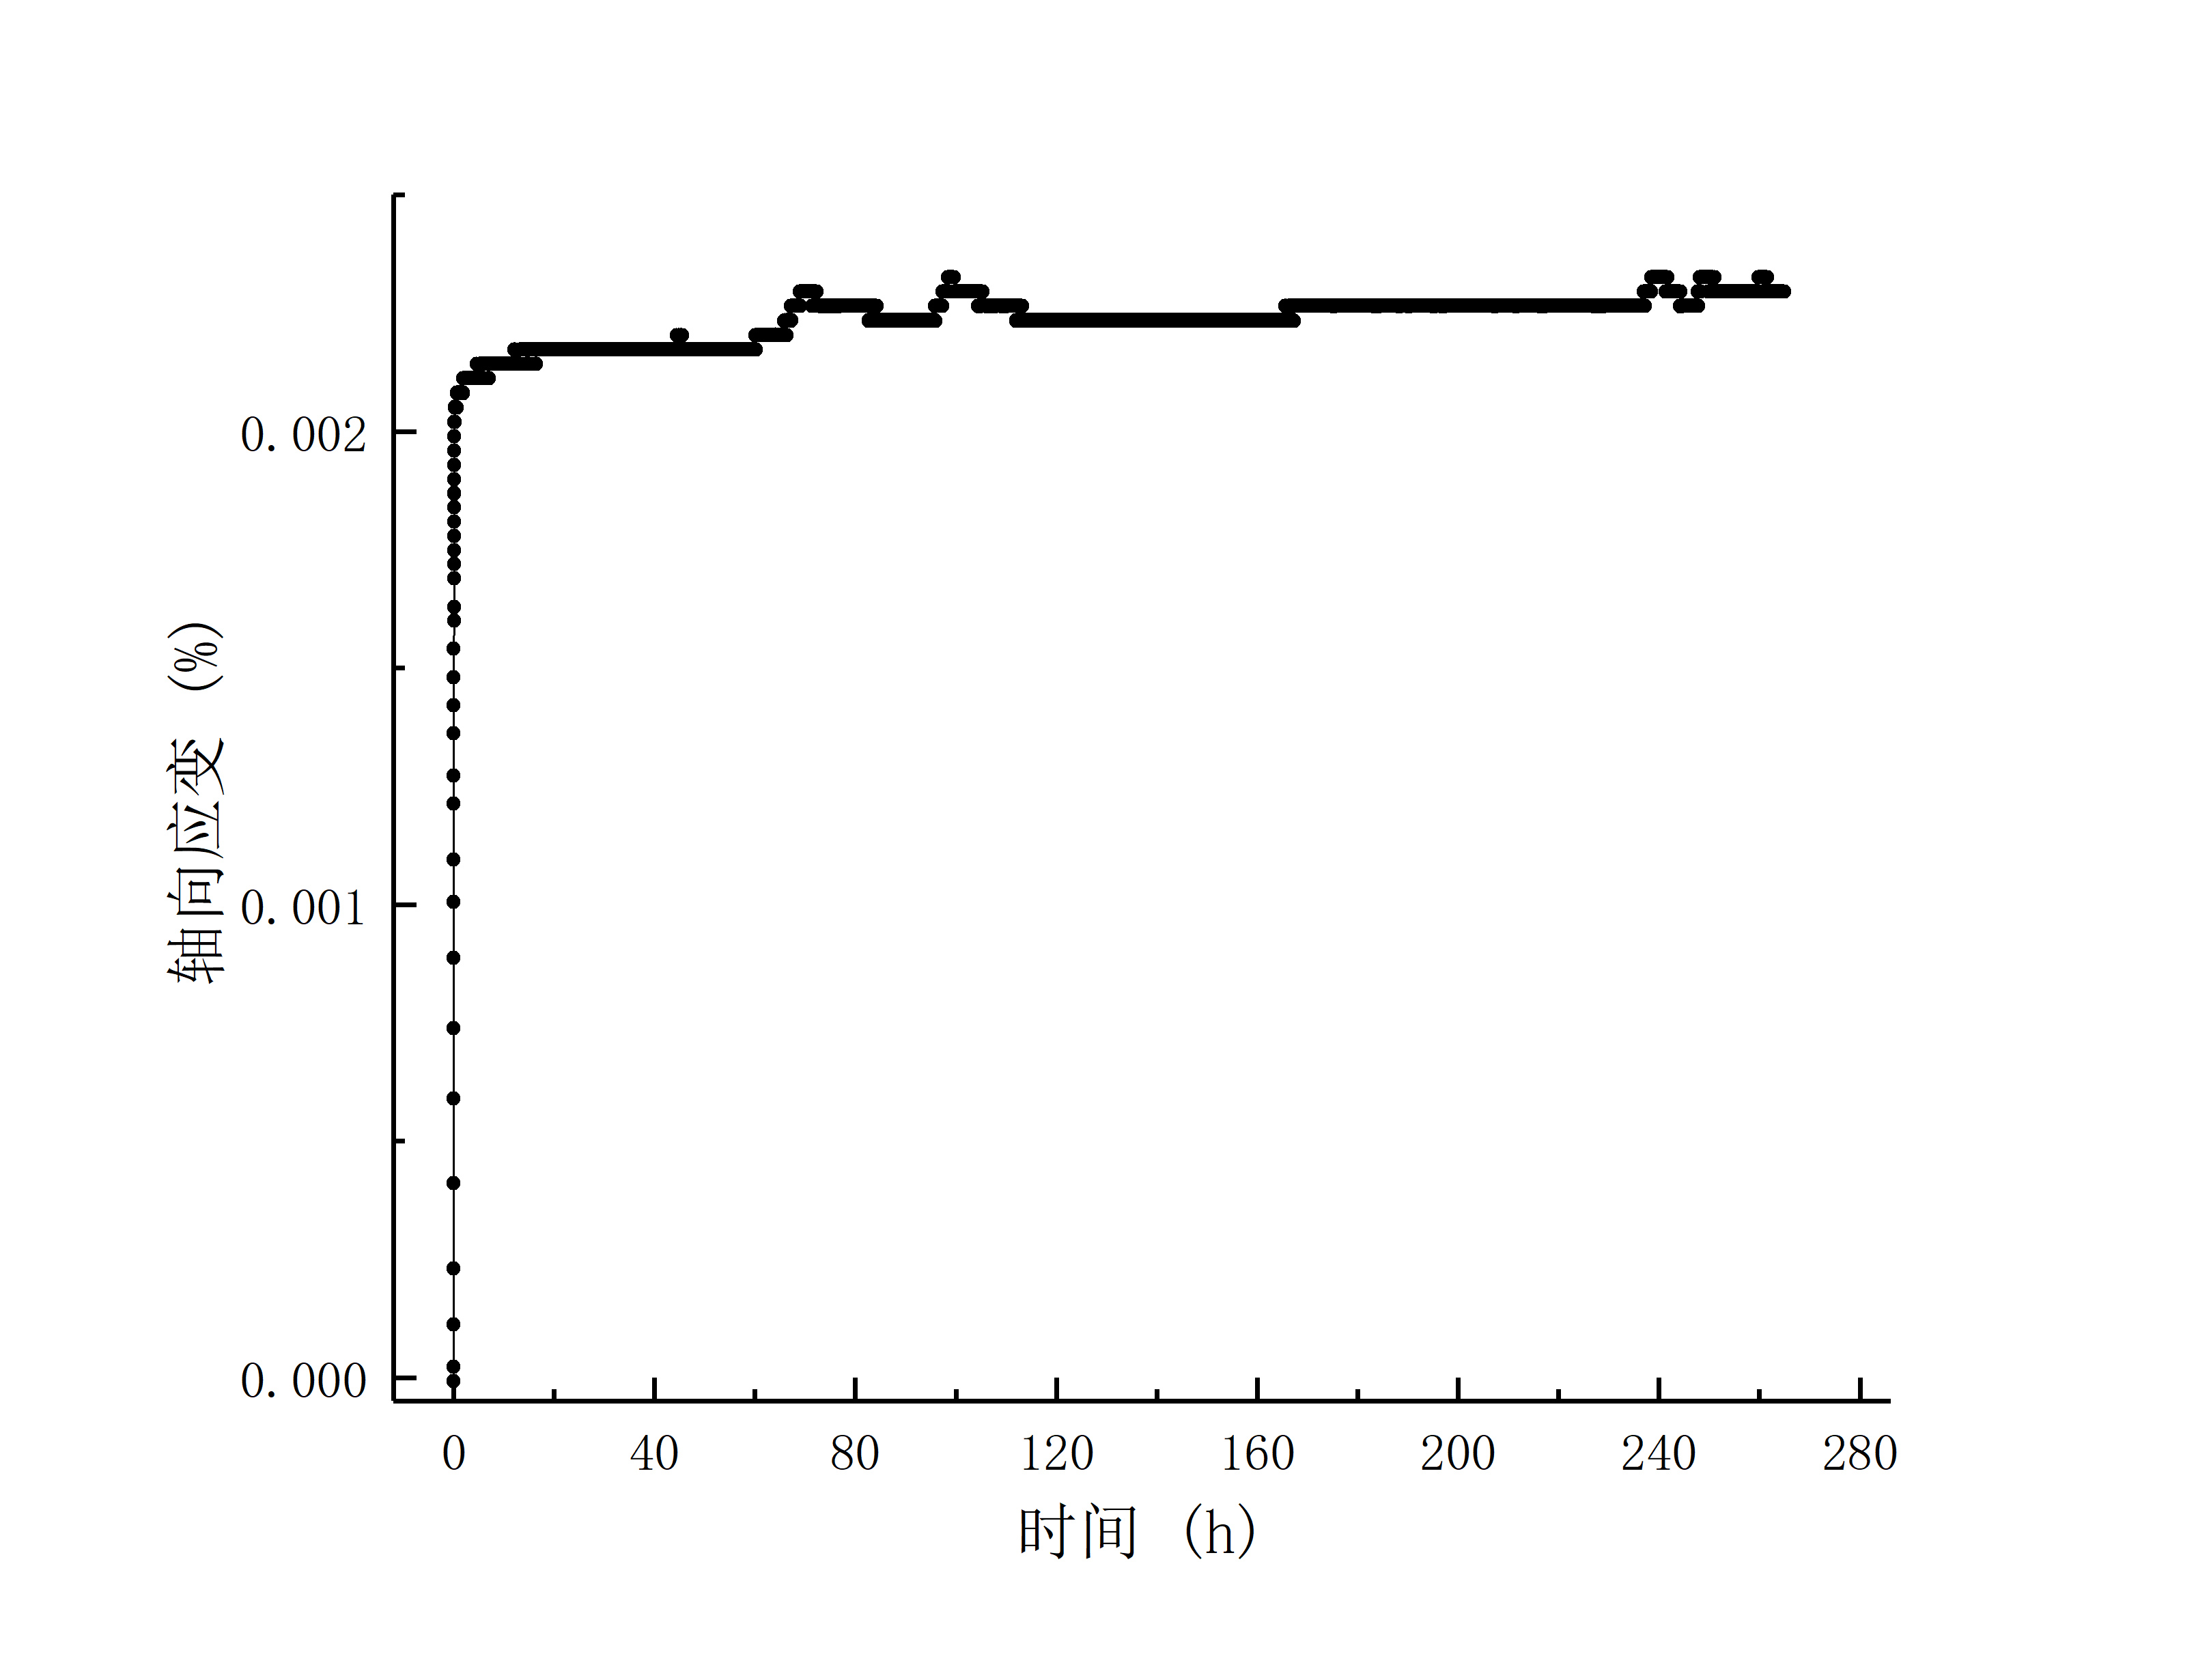
\includegraphics[width=1.1\textwidth]{img/chap2/C-04.png}
        \end{minipage}
    }
    \centering
    \subfigure[C-05]
    {
        \begin{minipage}{7cm}
            \centering
            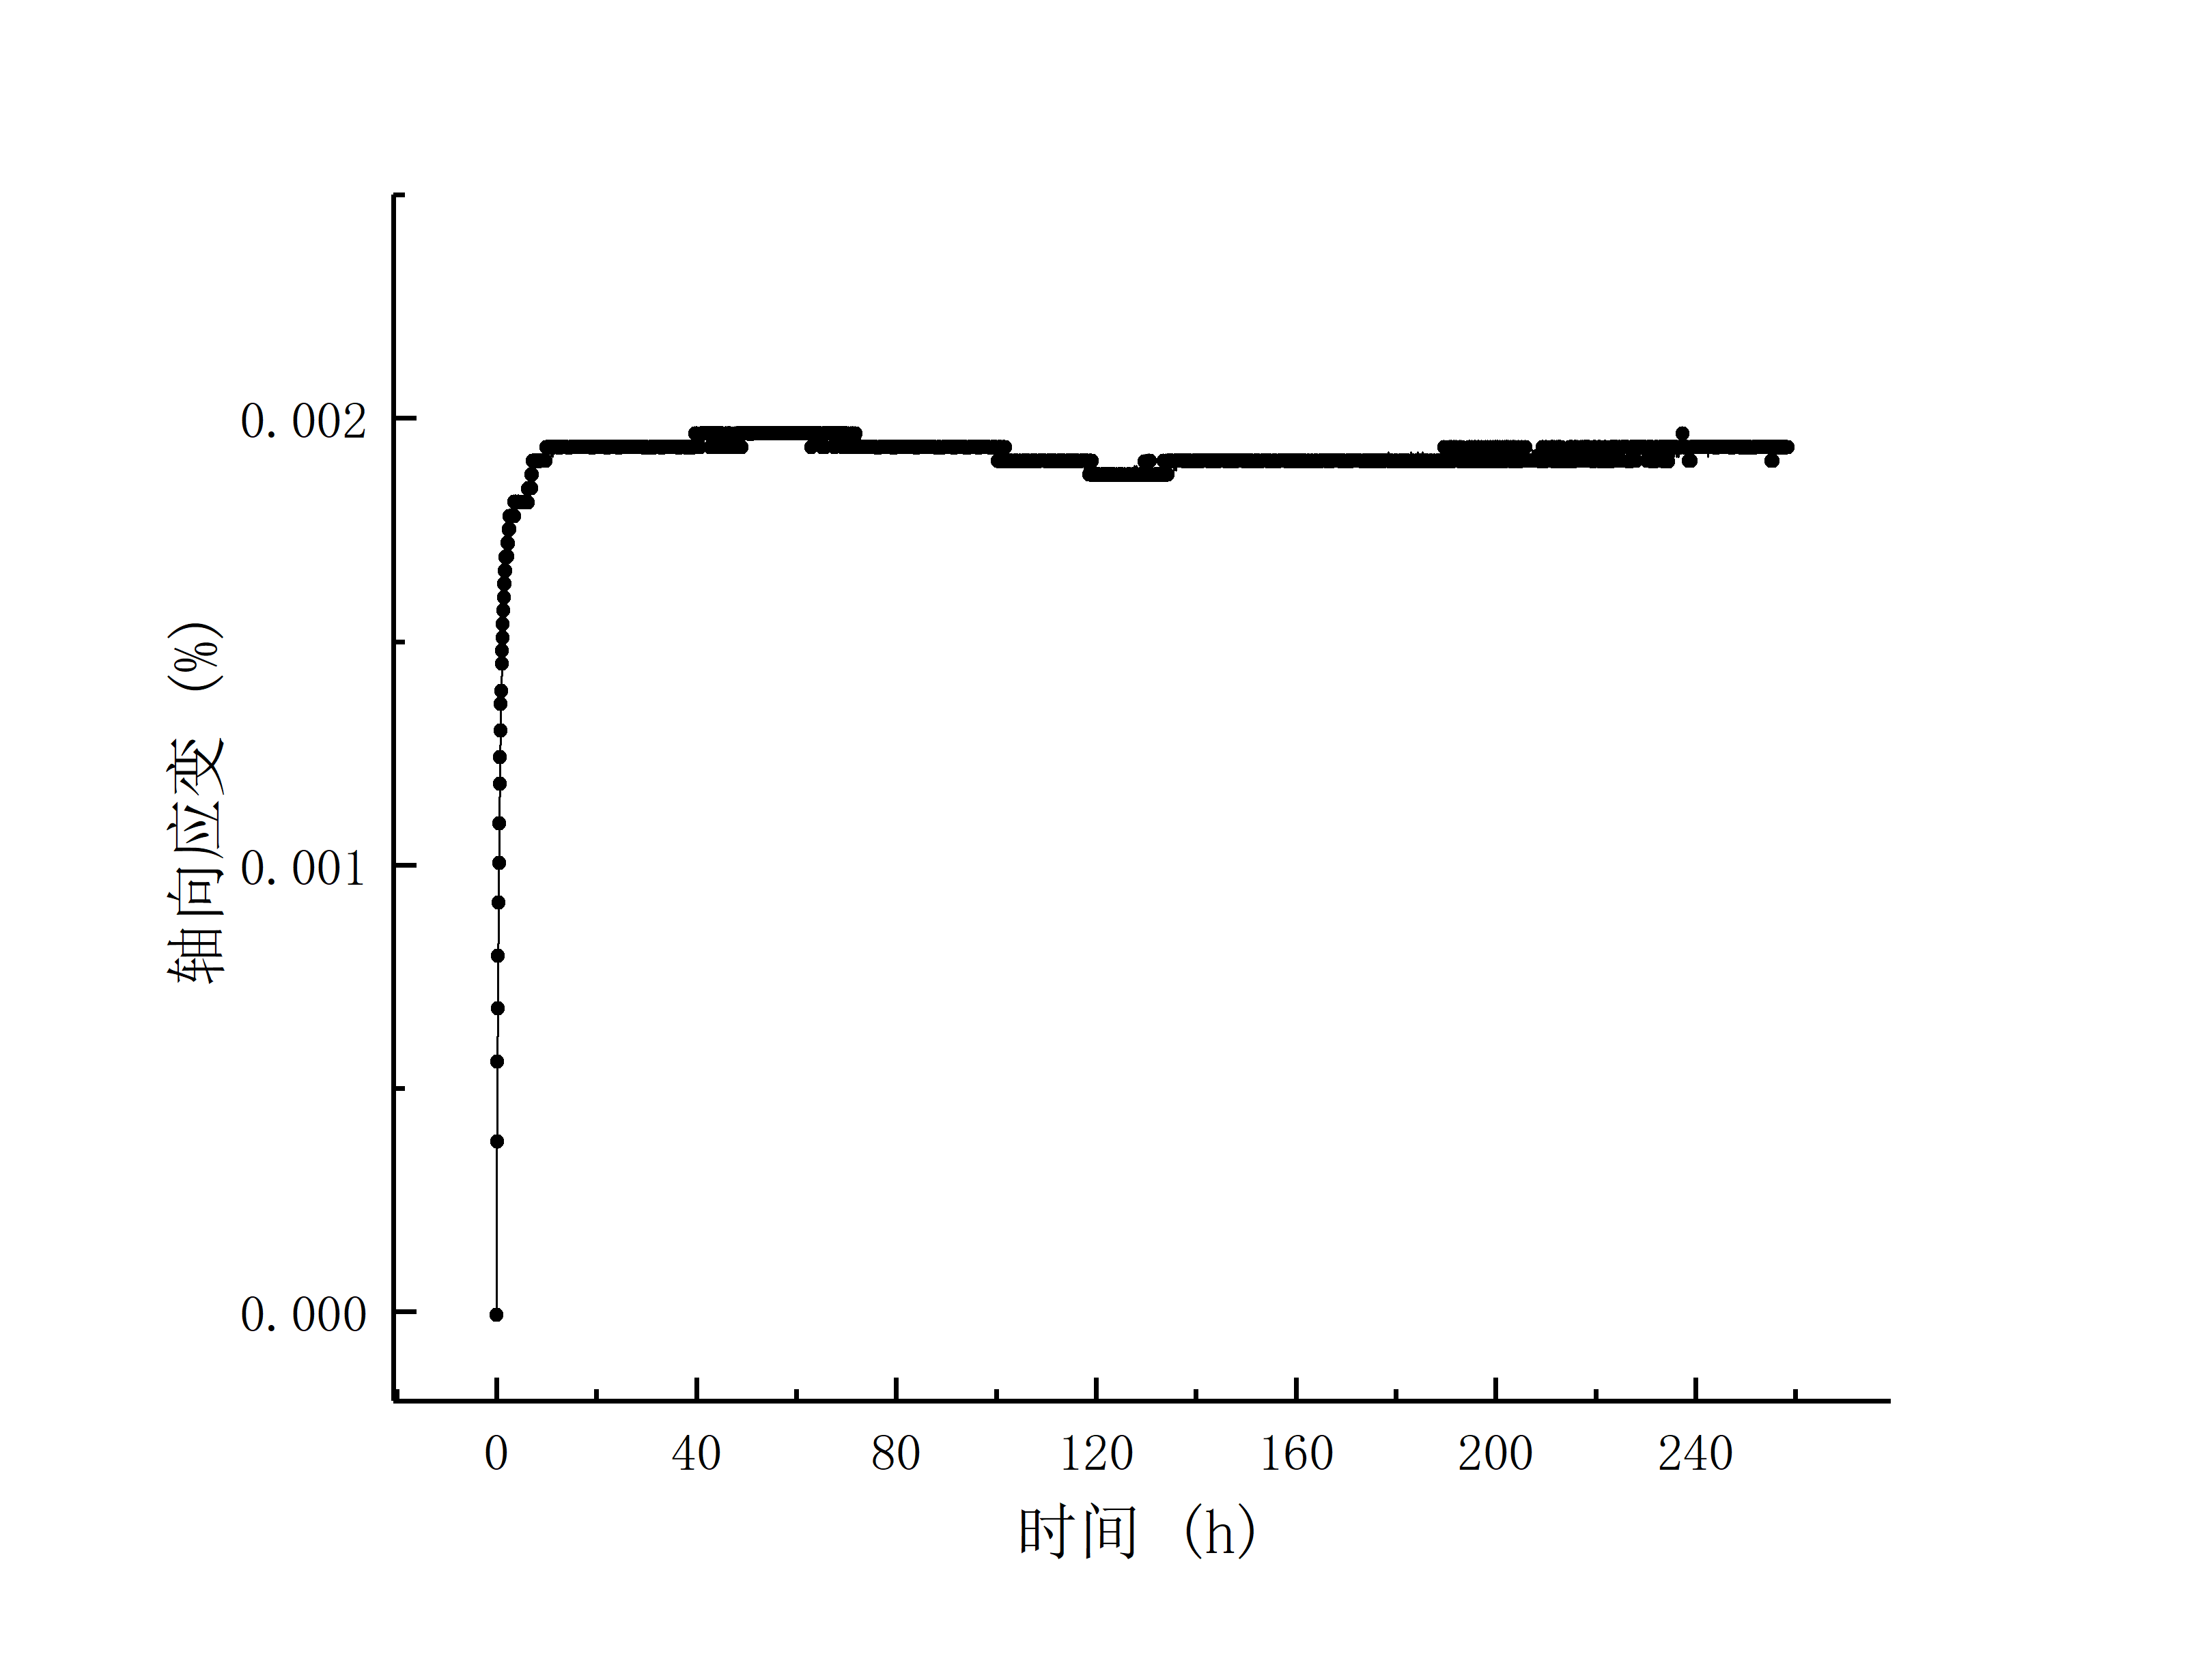
\includegraphics[width=1.1\textwidth]{img/chap2/C-05.png}
        \end{minipage}
    }
    \centering
    \caption{泥岩单轴压缩蠕变试验曲线图}
    \label{fig:2-9}
\end{figure}

\subsection{流变速率分析}
岩石的蠕变速率是描述岩石在恒定应力下变形快慢的物理量,也是研宄岩石蠕变特性的重要指标。分析蠕变试验数据,可以发现,在蠕变微段时间内蠕变速率波动大,这主要是由于岩样内部微观结构蠕变发展的非连续性所导致的。采用张春阳等\cite{张春阳}在文中分析深部斜长角闪岩蠕变速率的方法来计算泥岩蠕变试验分级加载过程中的蠕变速率
,在不影响速率趋势的情况下,选择$\Delta{t_i}$时间内n个蠕变数据,计算第n个和第n-1
个蠕变数据的差值(n>1),以此类推,求得各差值之和,这就是在$\Delta{t_i}$时间内试样的总蠕变量。将算出的第i段时间内的总蠕变量除以第i段的总时间,就可获得第i段时间内的螺变速率$v_i$,计算过程为如下:

\begin{equation}
  \left\{
  \begin{aligned}
 &\Delta{\varepsilon} =\Delta{\varepsilon_1}+\Delta{\varepsilon_2}+\cdots+\Delta{\varepsilon_{n-1}}  \\
 & \Delta{\varepsilon_1}=\varepsilon_2-\varepsilon_1,\Delta{\varepsilon_2}=\varepsilon_3-\varepsilon_2,\Delta{\varepsilon_{n-1}}=\varepsilon_n-\varepsilon_{n-1}\\ 
 & \Delta{\varepsilon}=(\varepsilon_2+\varepsilon_3+\cdots+\varepsilon_n)-(\varepsilon_1+\varepsilon_2+\cdots+\varepsilon_{n-1})=\varepsilon_n-\varepsilon_1  \\
 & {v_i}=\Delta{\varepsilon}/\Delta{t_i}
 \end{aligned}
 \right.
\end{equation}

其中,$\varepsilon_1,\varepsilon_2,\cdots,\varepsilon_n$为各段的轴向应变值;$\Delta{\varepsilon_1},\Delta{\varepsilon_2},\cdots,\Delta{\varepsilon_n}$是各微段轴向应变值之差,$\Delta{\varepsilon}$和$v_i$表示$\Delta{t_i}$时间段内的总应变和平均应变速率,将求得的相邻时间段内的应变速率连成曲线,各试样具体的流变速率如图~\ref{fig:2-10}所示:

\begin{figure}[ht!]
    \centering
    \subfigure[C-01]
    {
        \begin{minipage}{7cm}
            \centering
            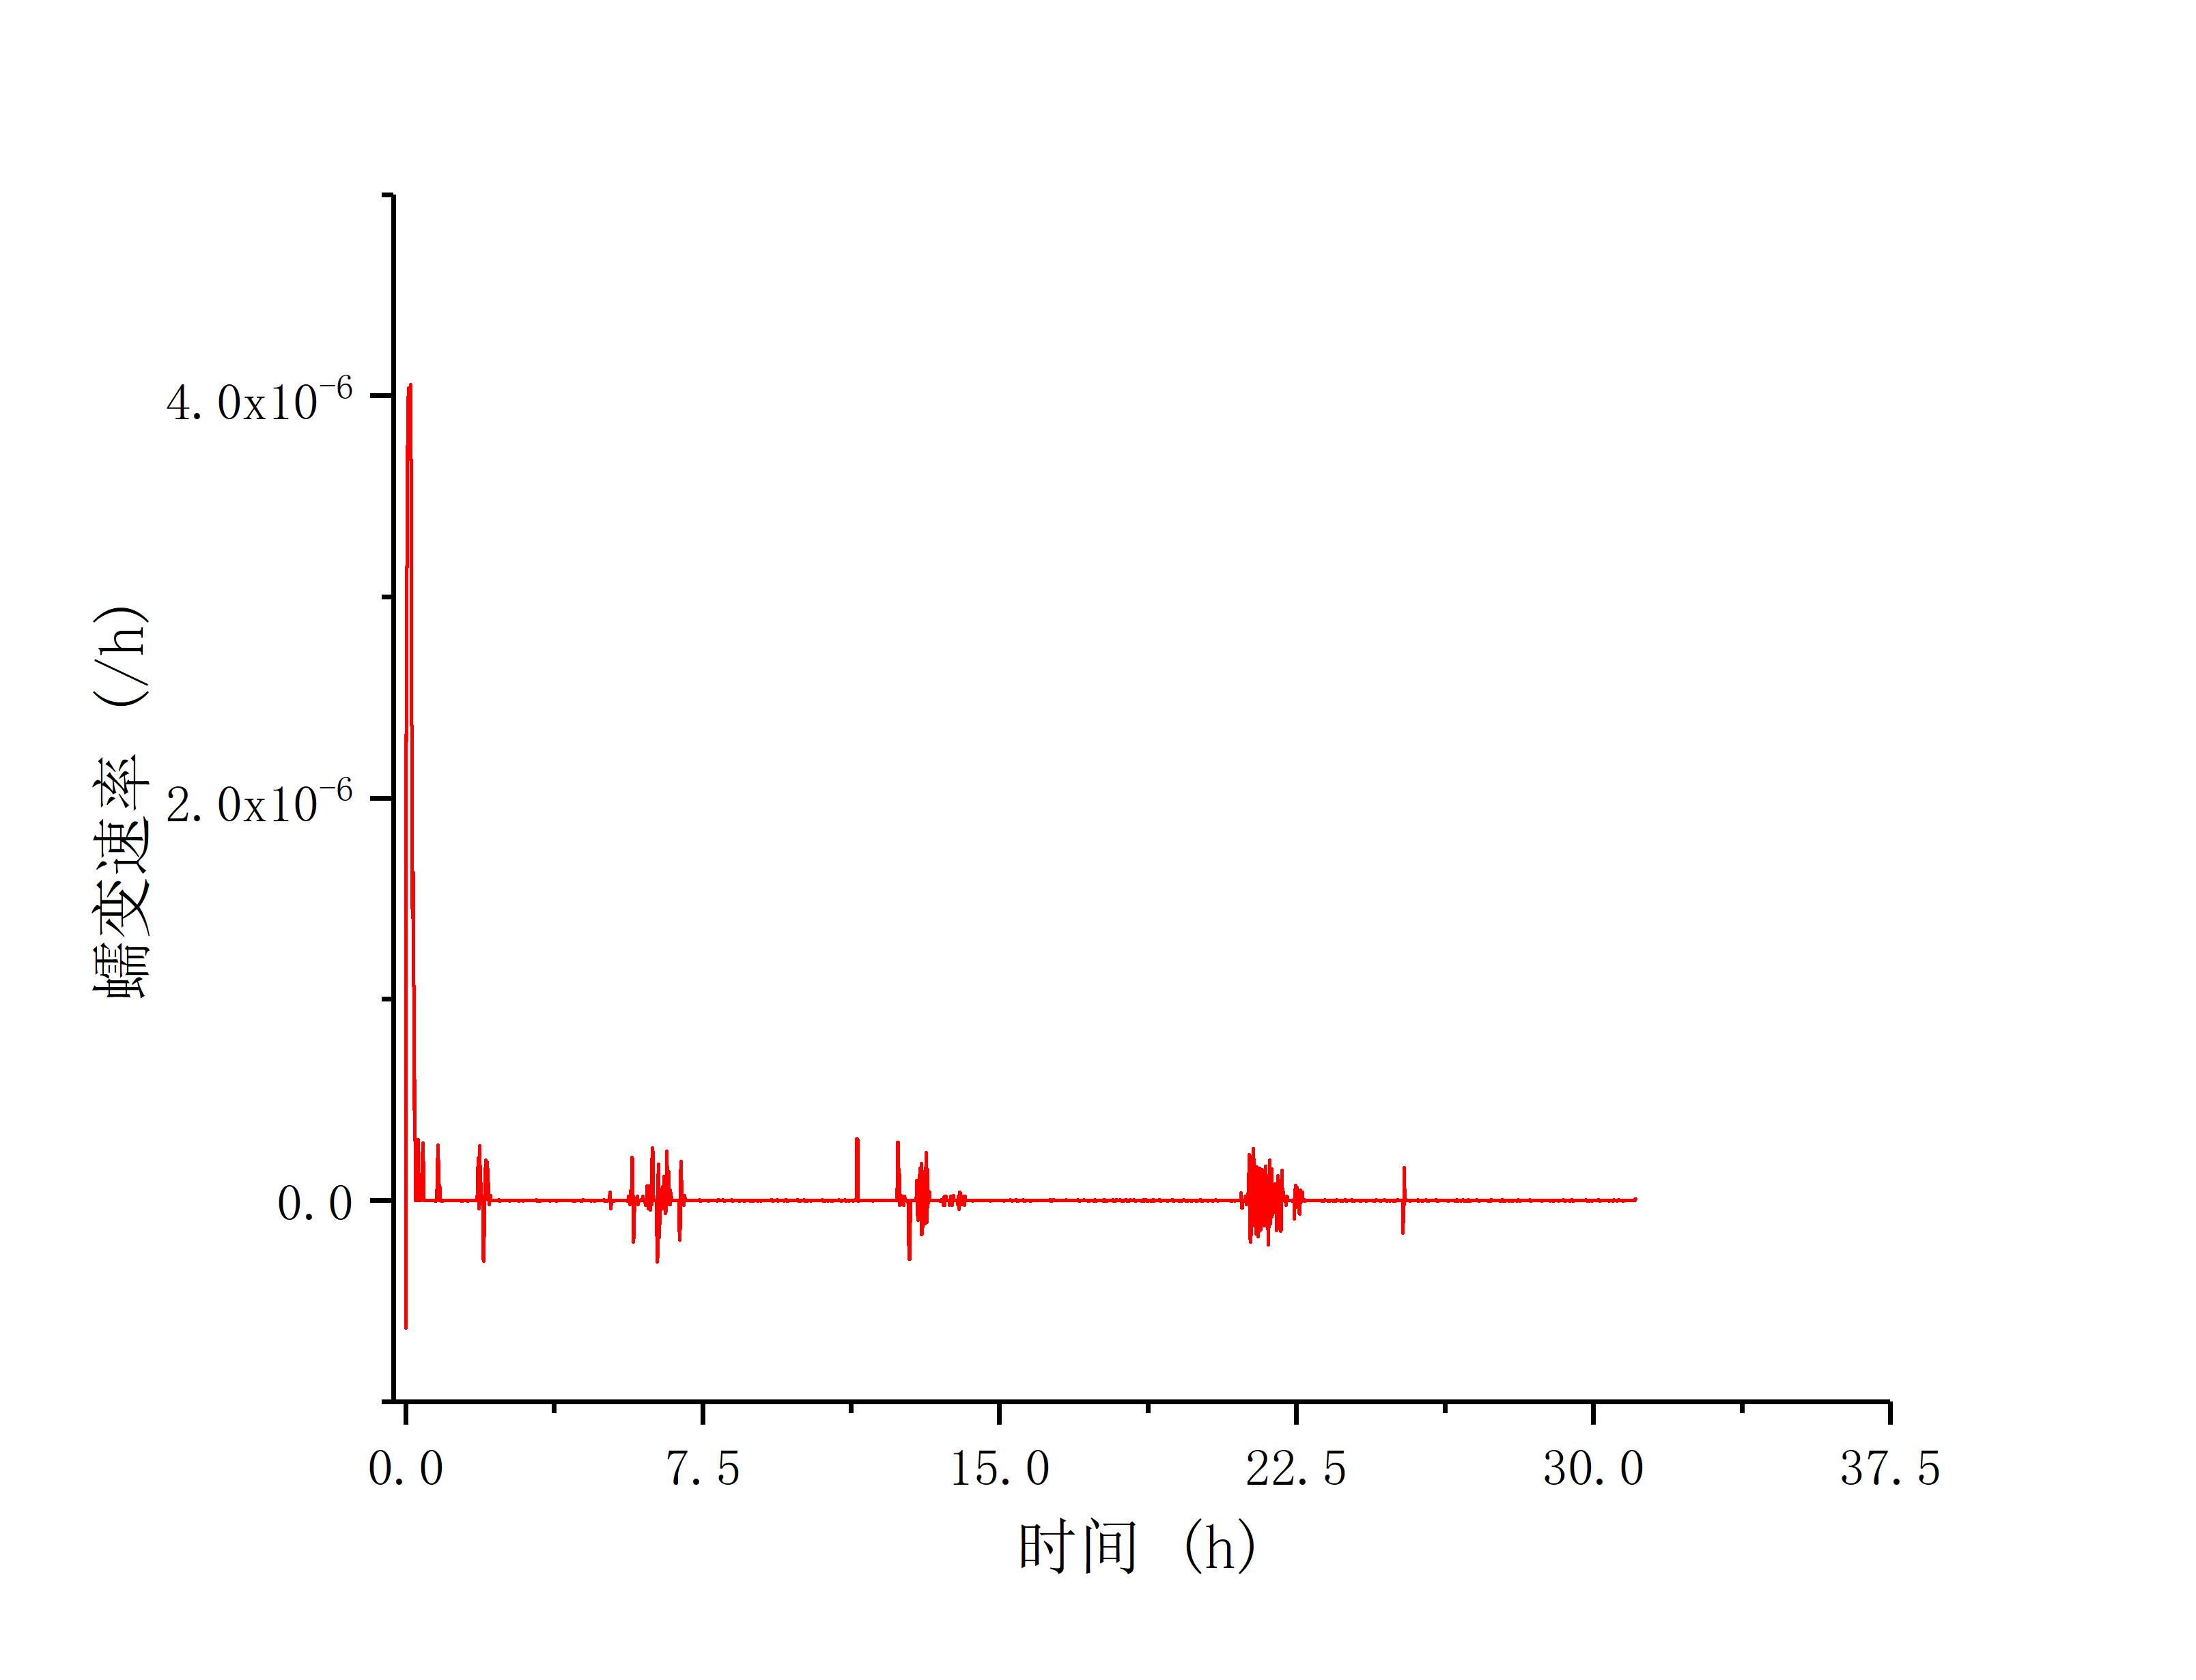
\includegraphics[width=1.1\textwidth]{img/chap2/C-01-v.png}
        \end{minipage}
    }
    \subfigure[C-02]
    {
        \begin{minipage}{7cm}
            \centering
            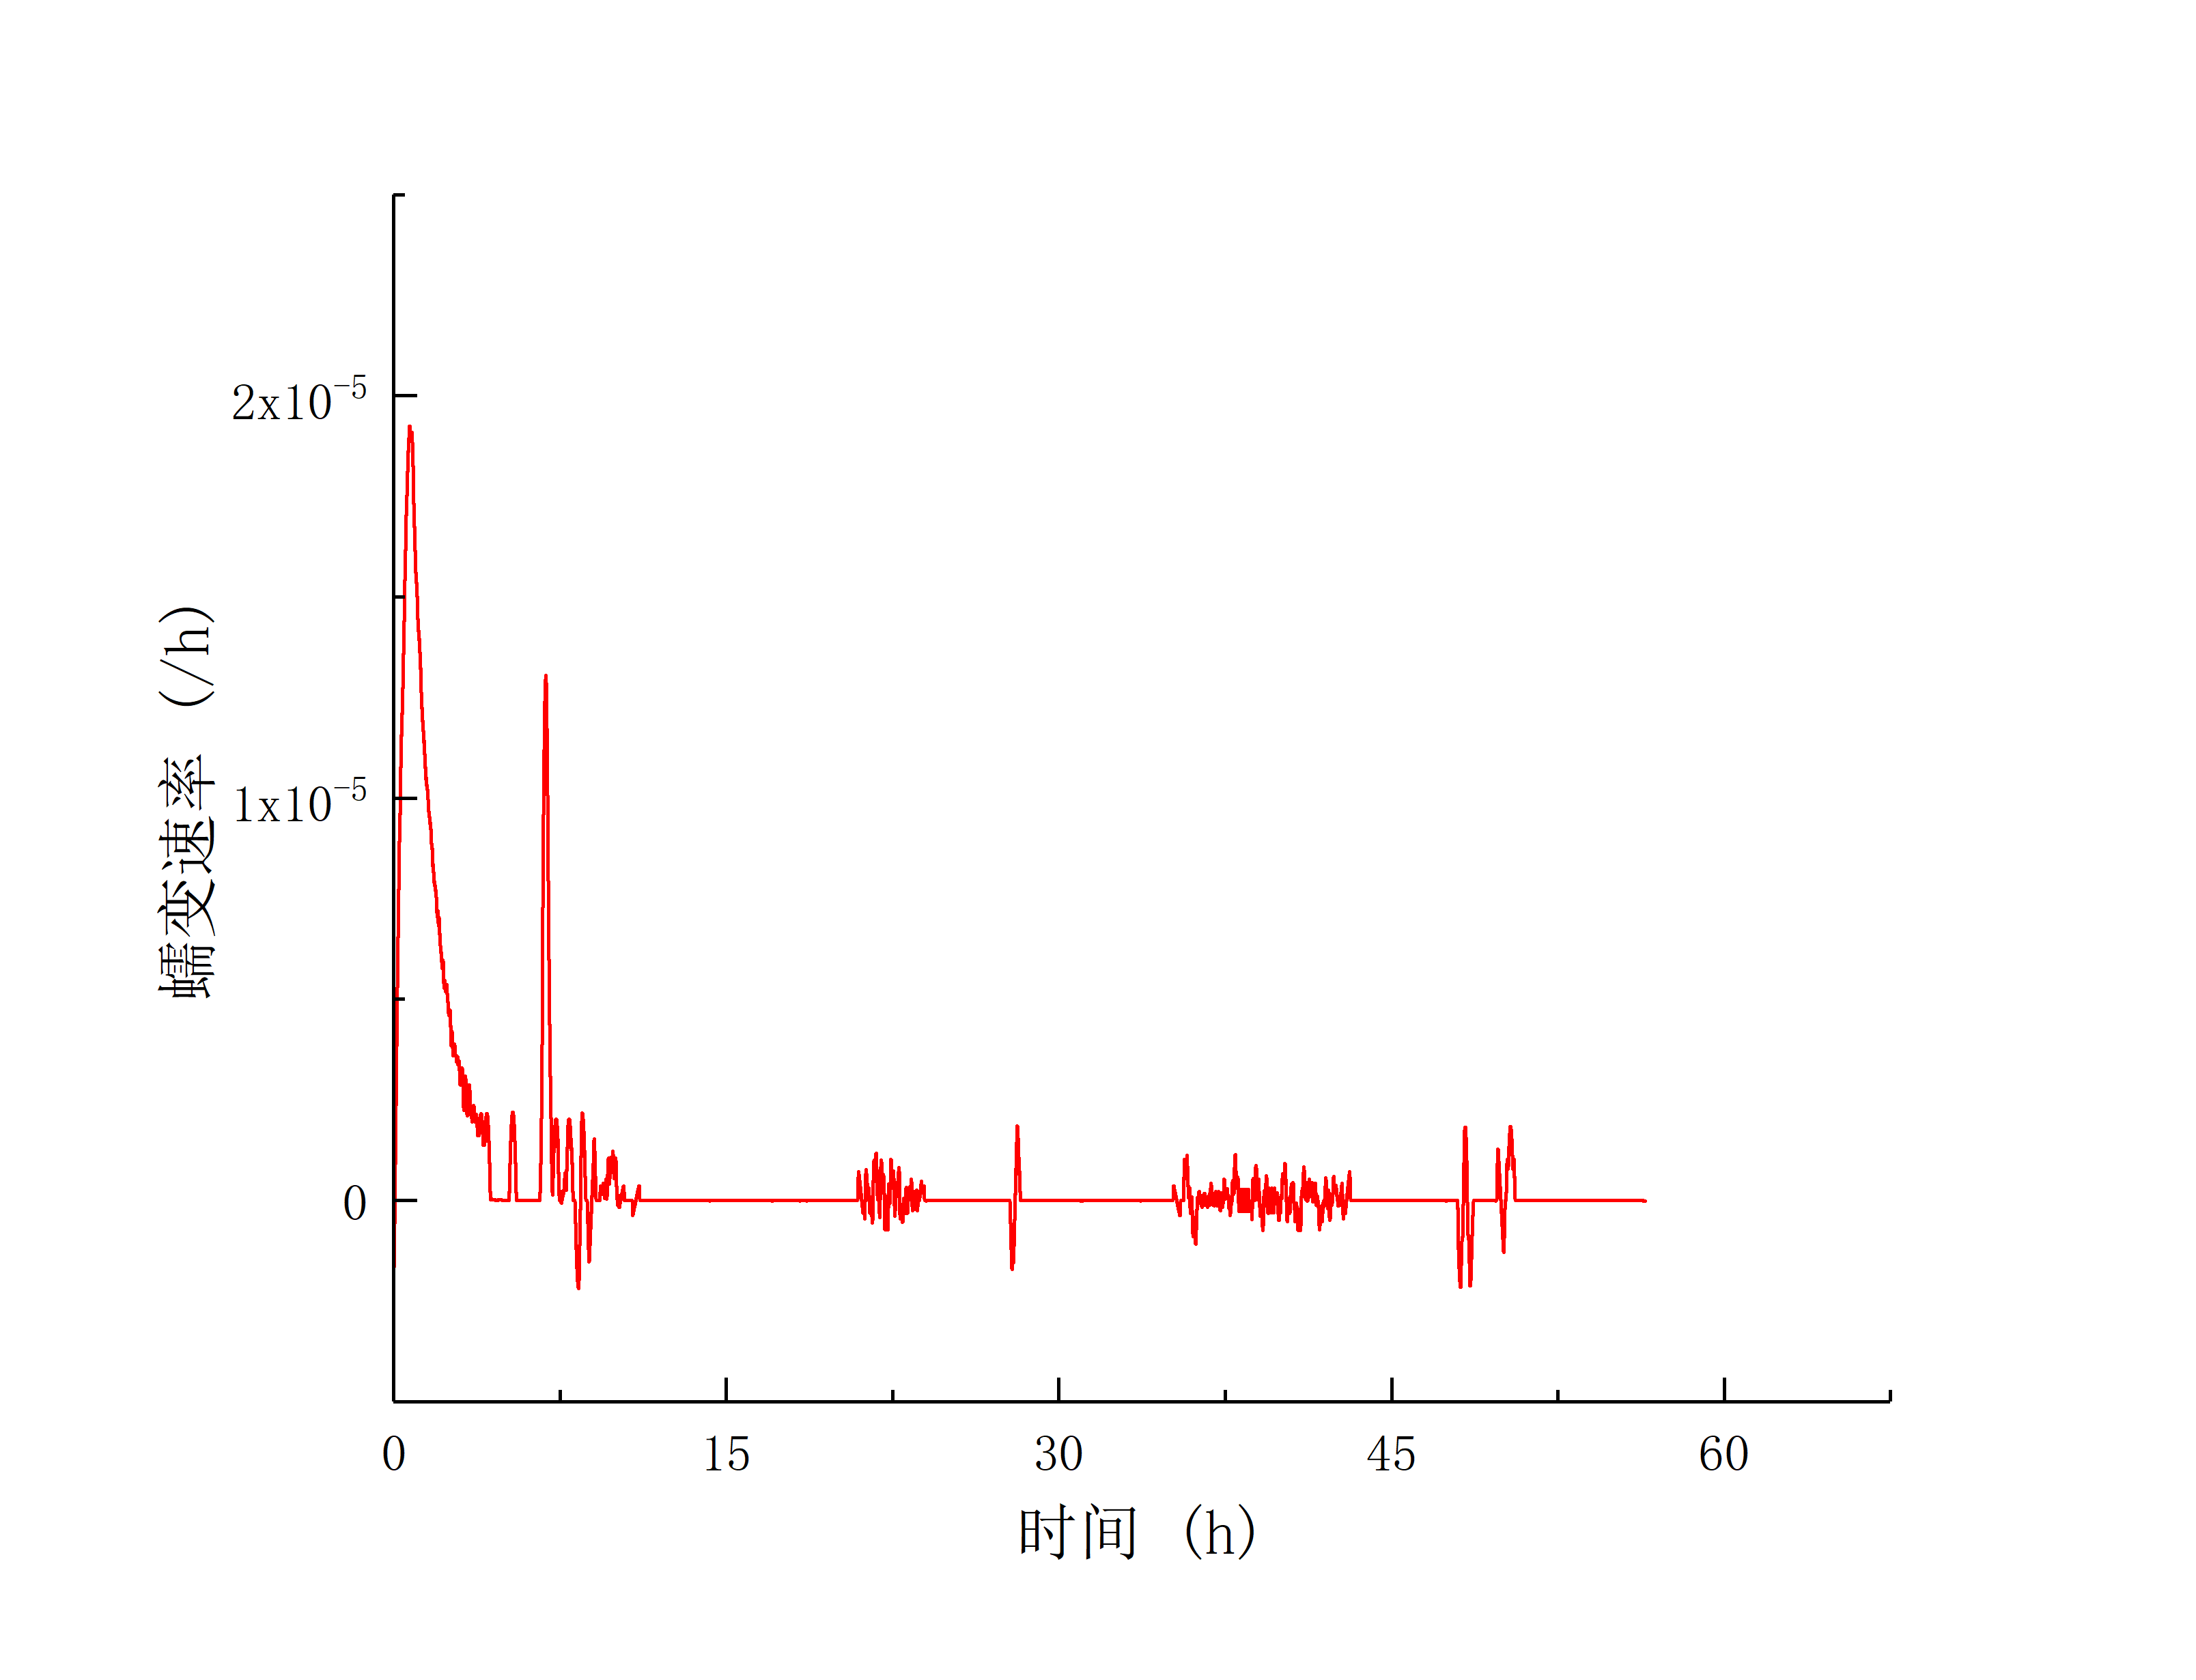
\includegraphics[width=1.1\textwidth]{img/chap2/C-02-v.png}
        \end{minipage}
    }
    \subfigure[C-04]
    {
        \begin{minipage}{7cm}
            \centering
            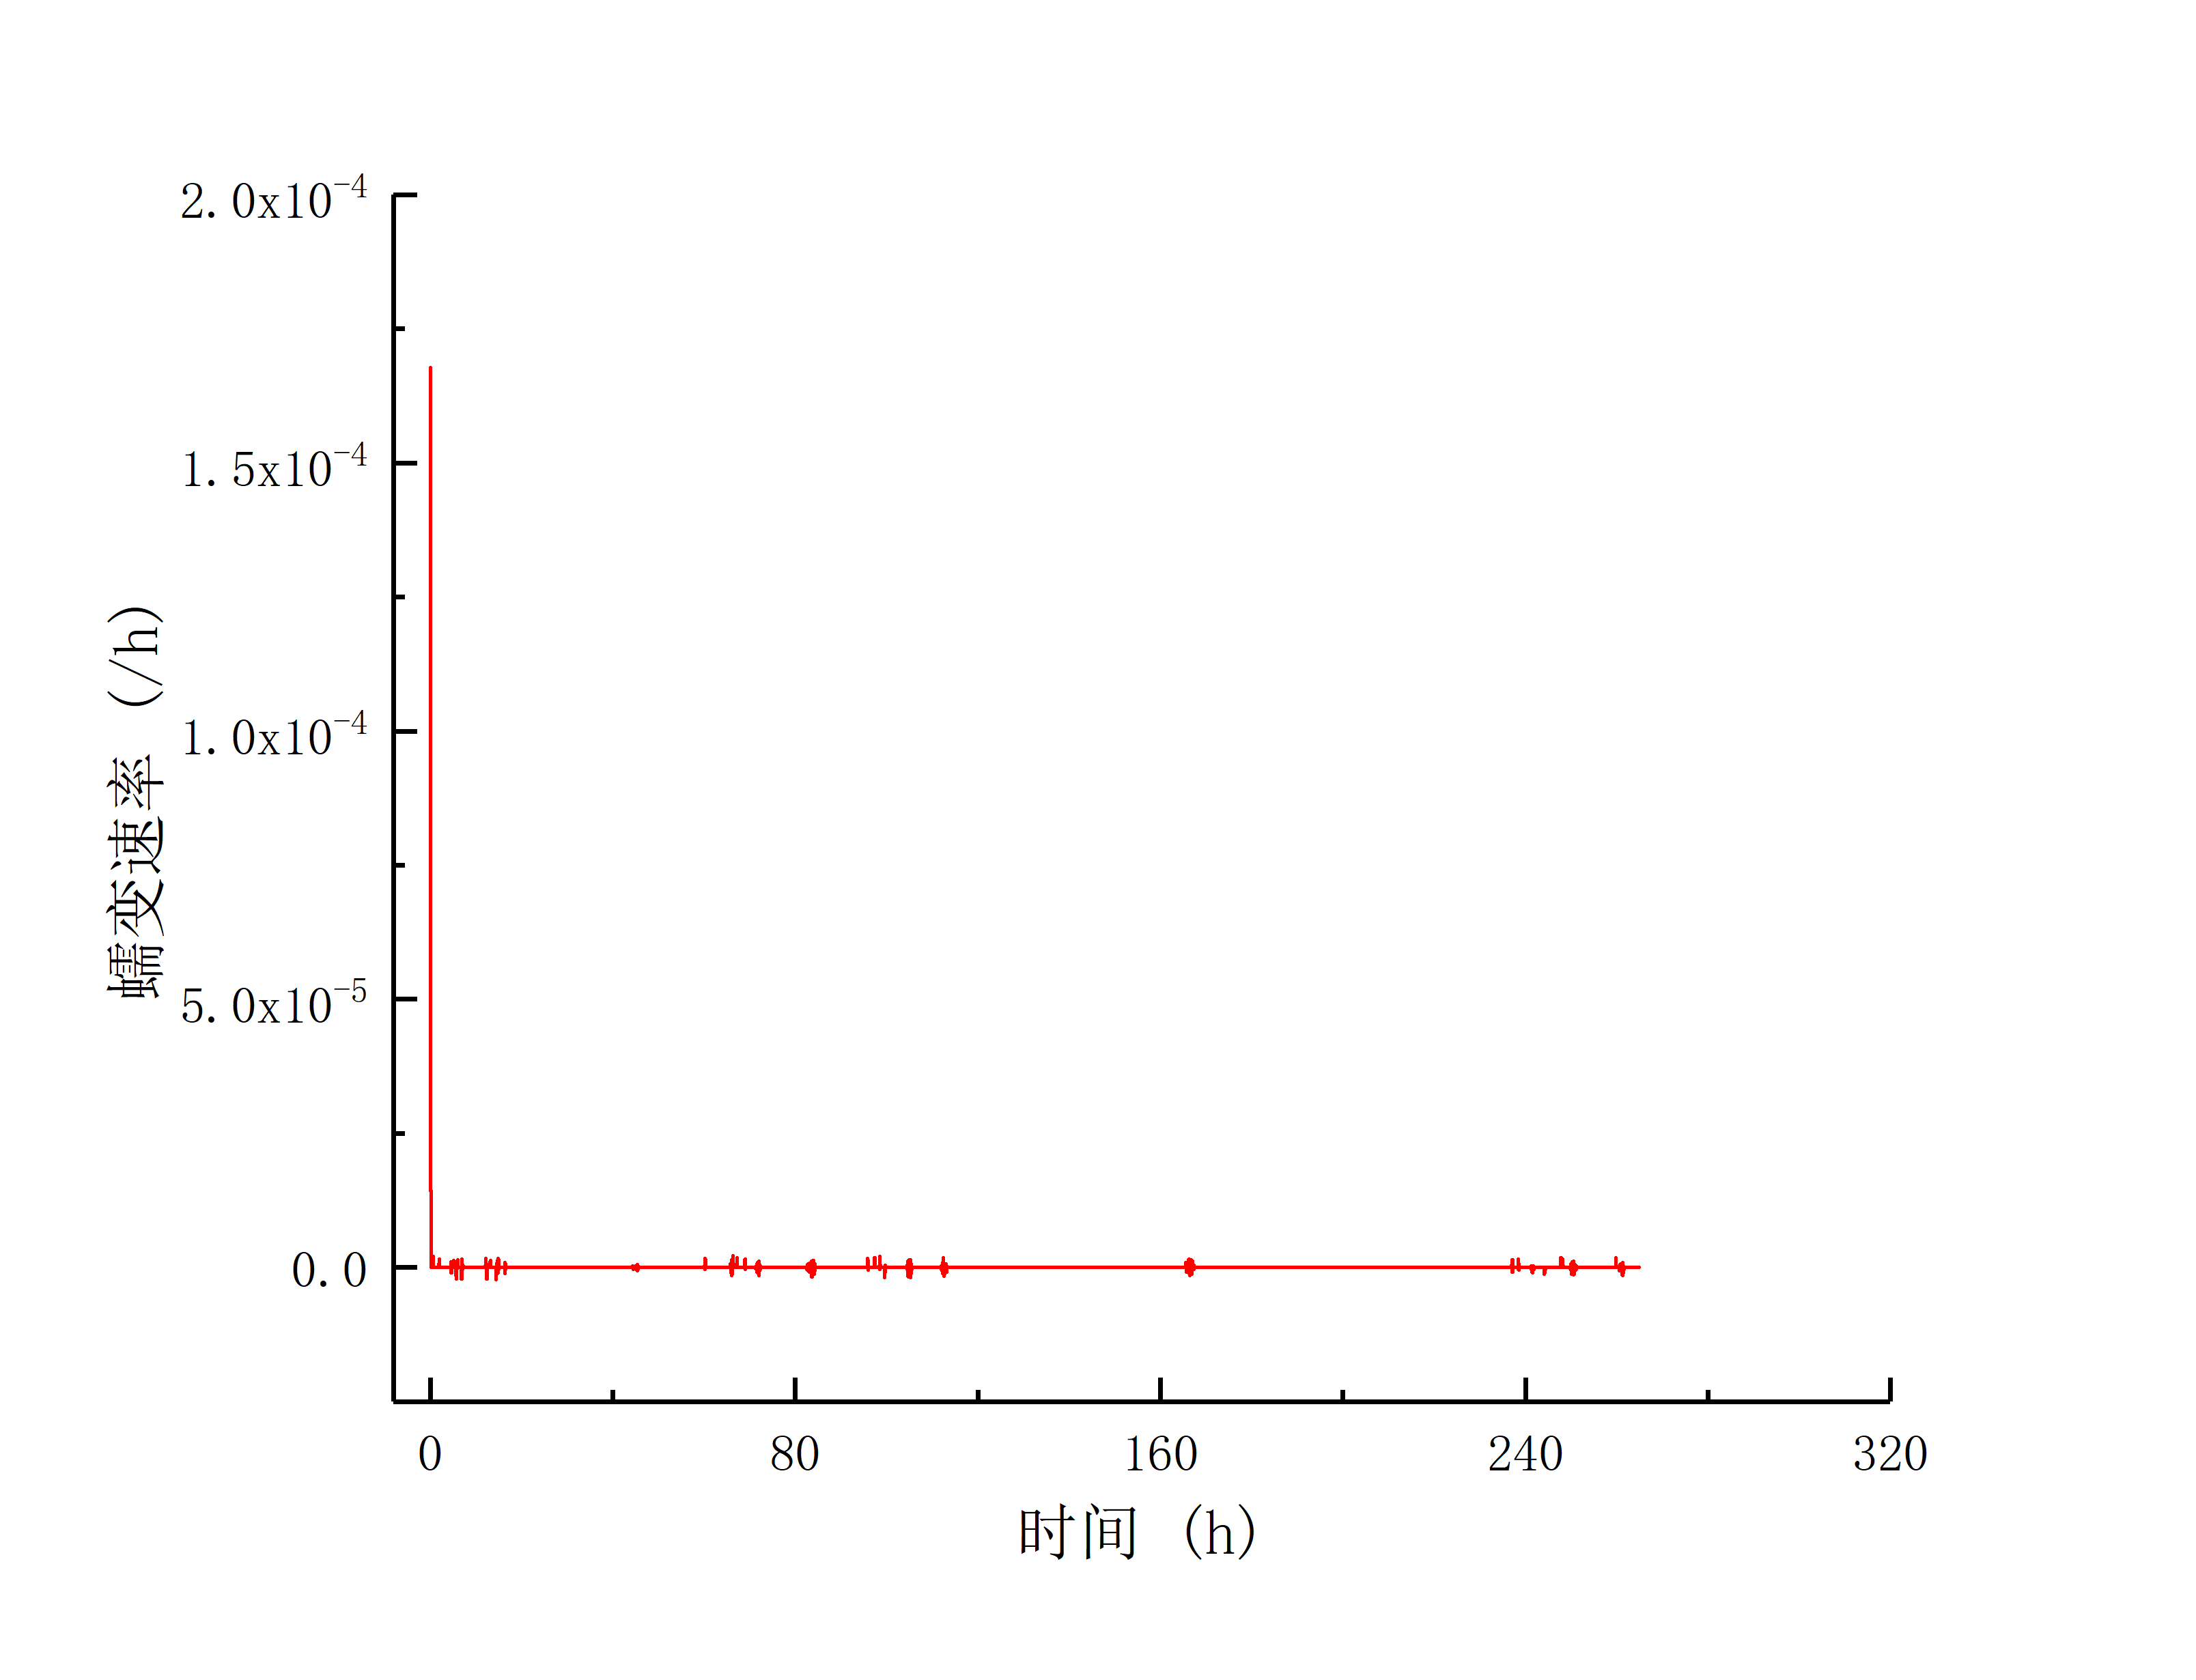
\includegraphics[width=1.1\textwidth]{img/chap2/C-04-v.png}
        \end{minipage}
    }
    \centering
    \subfigure[C-05]
    {
        \begin{minipage}{7cm}
            \centering
            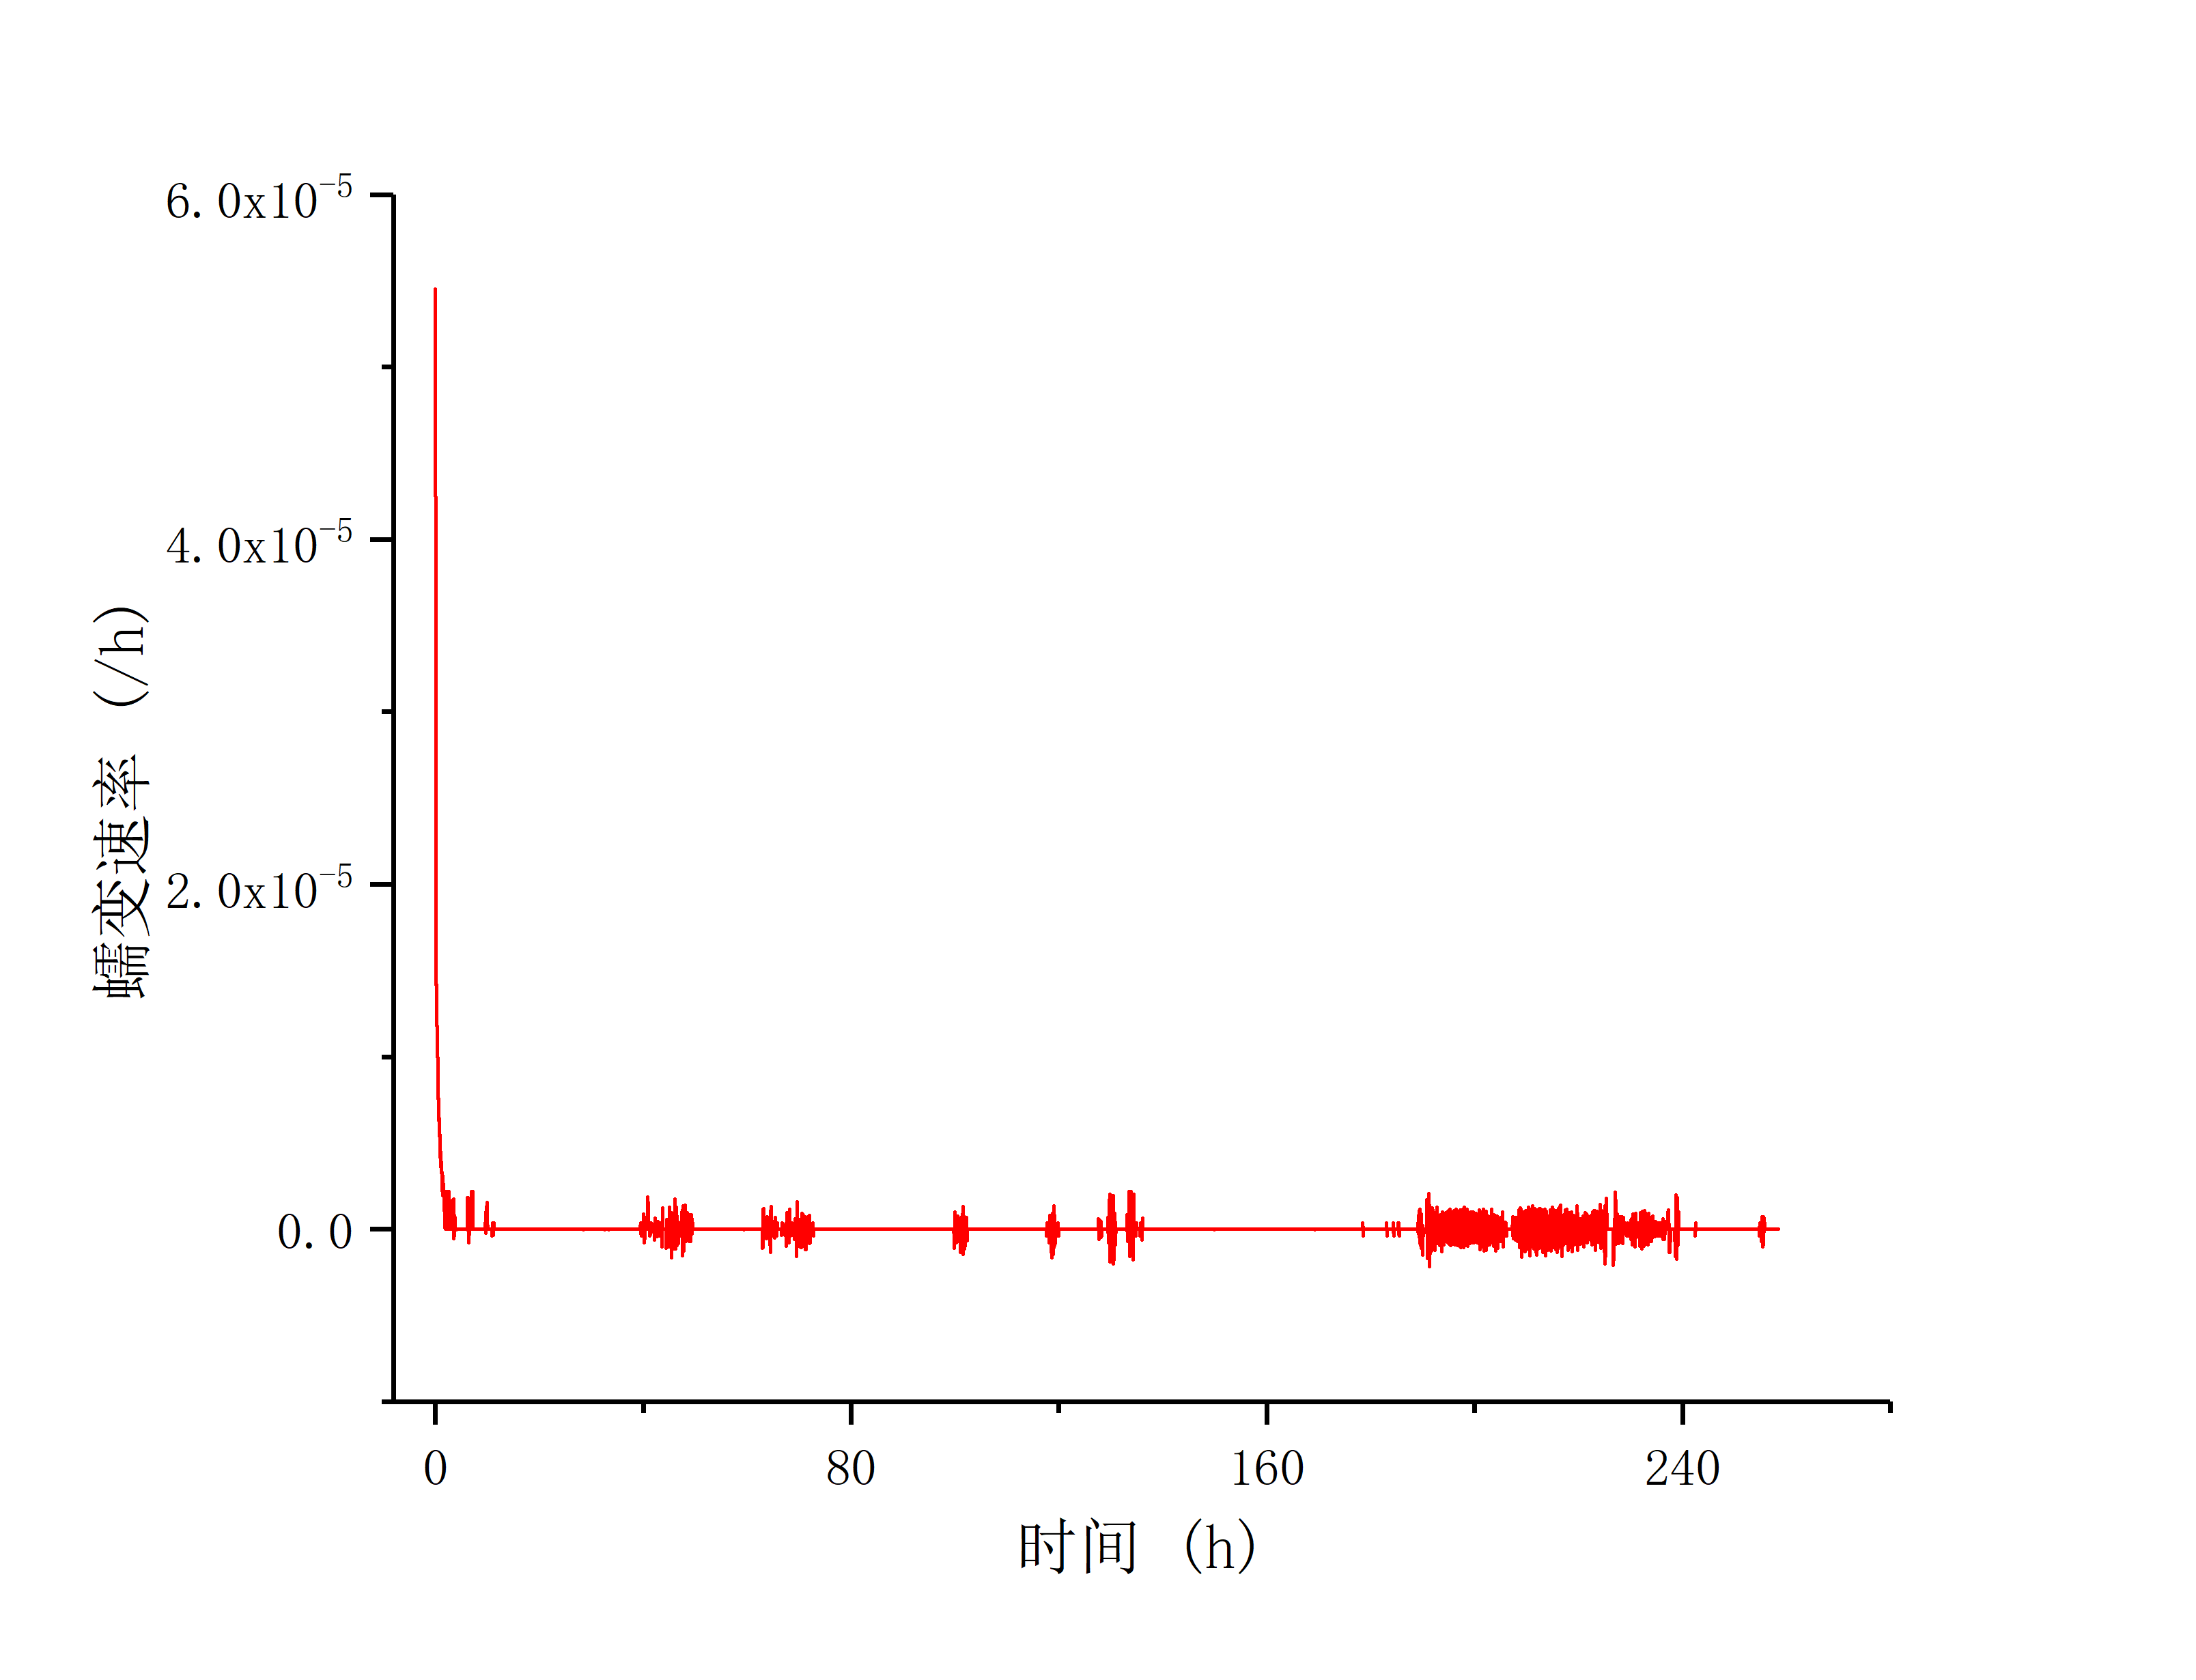
\includegraphics[width=1.1\textwidth]{img/chap2/C-05-v.png}
        \end{minipage}
    }
    \centering
    \caption{泥岩单轴压缩蠕变速率曲线图}
    \label{fig:2-10}
\end{figure}

以下四张图为单轴流变试验中试样流变速率的曲线图,C-03因为试样很快破坏,因此不进行流变速率分析。
在流变试验中,施加一定的应力值,在试样进入流变阶段后,首先会进入流变速率不断减小的衰减蠕变阶段,
从图中我们可以看出,在瞬时应变发生到流变变形开始前的这个短暂的时间内,随着瞬时应变的增大,流变速率会快速增长至最大值。之后,在初始蠕变阶段,流变速率会随着时间的增长逐渐减小的,并且在初始阶段都衰减的十分迅速,不断发展趋于与横轴平行的近似直线,当流变速率衰减到某一定值时,流变进入稳定发展阶段,
若施加的初始应力较小,蠕变速率会一直减小到无限接近于零,如果施加的应力较大,试样的蠕变速率则会减小到某一非零的常数并保持不变,此对应的流变速率为稳态流变速率,试样的蠕变变形随着时间稳定增加。

由图我们可以看出,岩石在蠕变过程中的大多数时间都是处于稳定蠕变阶段,在这个过程中,岩石的变形逐步积累,内部裂隙不断发展,直至试样破坏。总体来说,相同岩石的初始蠕变速率及稳态蠕变速率随着应力水平的增大而增大,不过在单轴蠕变试验采取的是分别加载的方法,所以试样之间存在差异,导致像分级加载一样准确反应一个试样在不同加载等级下的流变过程与变化规律。当然,由于局部非均匀破裂的影响,泥岩试样在一定应力水平条件下的稳态流变速率会有一定的波动。




\section{泥岩三轴流变试验}
三轴流变试验则是为了研究围压的变化对岩石流变过程应力-应变的影响。选取了三个试样分别编号,测量其具体物理参数,考虑到蠕变试验的时间较长,且制备的试样在进行蠕变试验前还需进行常规三轴压缩试验,试样的数量有限,因此本次三轴流变试验均采用分级加载的方法研究岩石流变特性。泥岩三轴流变试验安排如下表~\ref{tab:泥岩三轴蠕变试验工况表}所示:

\begin{table}[ht!]\small
    \centering
    \begin{threeparttable}
    \begin{tabular}{p{3cm}<{\centering} p{3cm}<{\centering} p{3cm}<{\centering} p{3cm}<{\centering}}
        \toprule
        试样编号  & 围压(MPa)  &  加载等级   &  加载时间(h)\\
        \midrule
                    &    &   0.7$\sigma_\mathrm{F}$   &  24   \\ 
                    &    &   0.7$5\sigma_\mathrm{F}$  &  48   \\ 
        D-01       &  5 &   0.8$\sigma_\mathrm{F}$   &  48  \\
                    &    &   0.85$\sigma_\mathrm{F}$  &  24  \\
                    &    &   0.9$\sigma_\mathrm{F}$  &  24  \\
                    &    &   0.95$\sigma_\mathrm{F}$  &  压至破坏  \\ 
        \midrule
                    &    &   0.7$\sigma_\mathrm{F}$   &  24   \\ 
                    &    &   0.75$\sigma_\mathrm{F}$  &  48   \\ 
        D-02        &  10 &   0.8$\sigma_\mathrm{F}$   &  48  \\
                    &    &   0.85$\sigma_\mathrm{F}$  &  24  \\
                    &    &   0.9$\sigma_\mathrm{F}$  &  24  \\
                    &    &   0.95$\sigma_\mathrm{F}$  &  压至破坏  \\
        \midrule
                    &    &   0.7$\sigma_\mathrm{F}$   &  24   \\ 
                    &    &   0.75$\sigma_\mathrm{F}$  &  48   \\ 
        D-03        &  10 &   0.8$\sigma_\mathrm{F}$   &  48  \\
                    &    &   0.85$\sigma_\mathrm{F}$  &  24  \\
                    &    &   0.9$\sigma_\mathrm{F}$  &  24  \\
                    &    &   0.95$\sigma_\mathrm{F}$  &  压至破坏  \\
        \bottomrule
    \end{tabular}
     \begin{tablenotes}    
        \footnotesize               
        \item 注:$\sigma_F$为三轴压缩试验测得的岩石峰值强度
     \end{tablenotes}            
    \end{threeparttable}       
    \caption{泥岩三轴蠕变试验工况表}
    \label{tab:泥岩三轴蠕变试验工况表}
\end{table}

在三轴流变试验中,我们采用分级加载的方式。在流变实验结束后,我们对收集到的时间、应力、应变数据进行处理,绘制得到单个试样在不同应力等级下的阶梯状时间-应变曲线如图\ref{fig:2-11}所示。各试样在每一级应力加载下均出现流变速率随时间减小的衰减蠕变阶段和流变速率近似不变的稳态蠕变阶段,随着加载应力等级的提高,流变变形量总体呈增加的趋势。


\begin{figure}[ht!]
    \centering
    \subfigure[D-01]
    {
        \begin{minipage}{7cm}
            \centering
            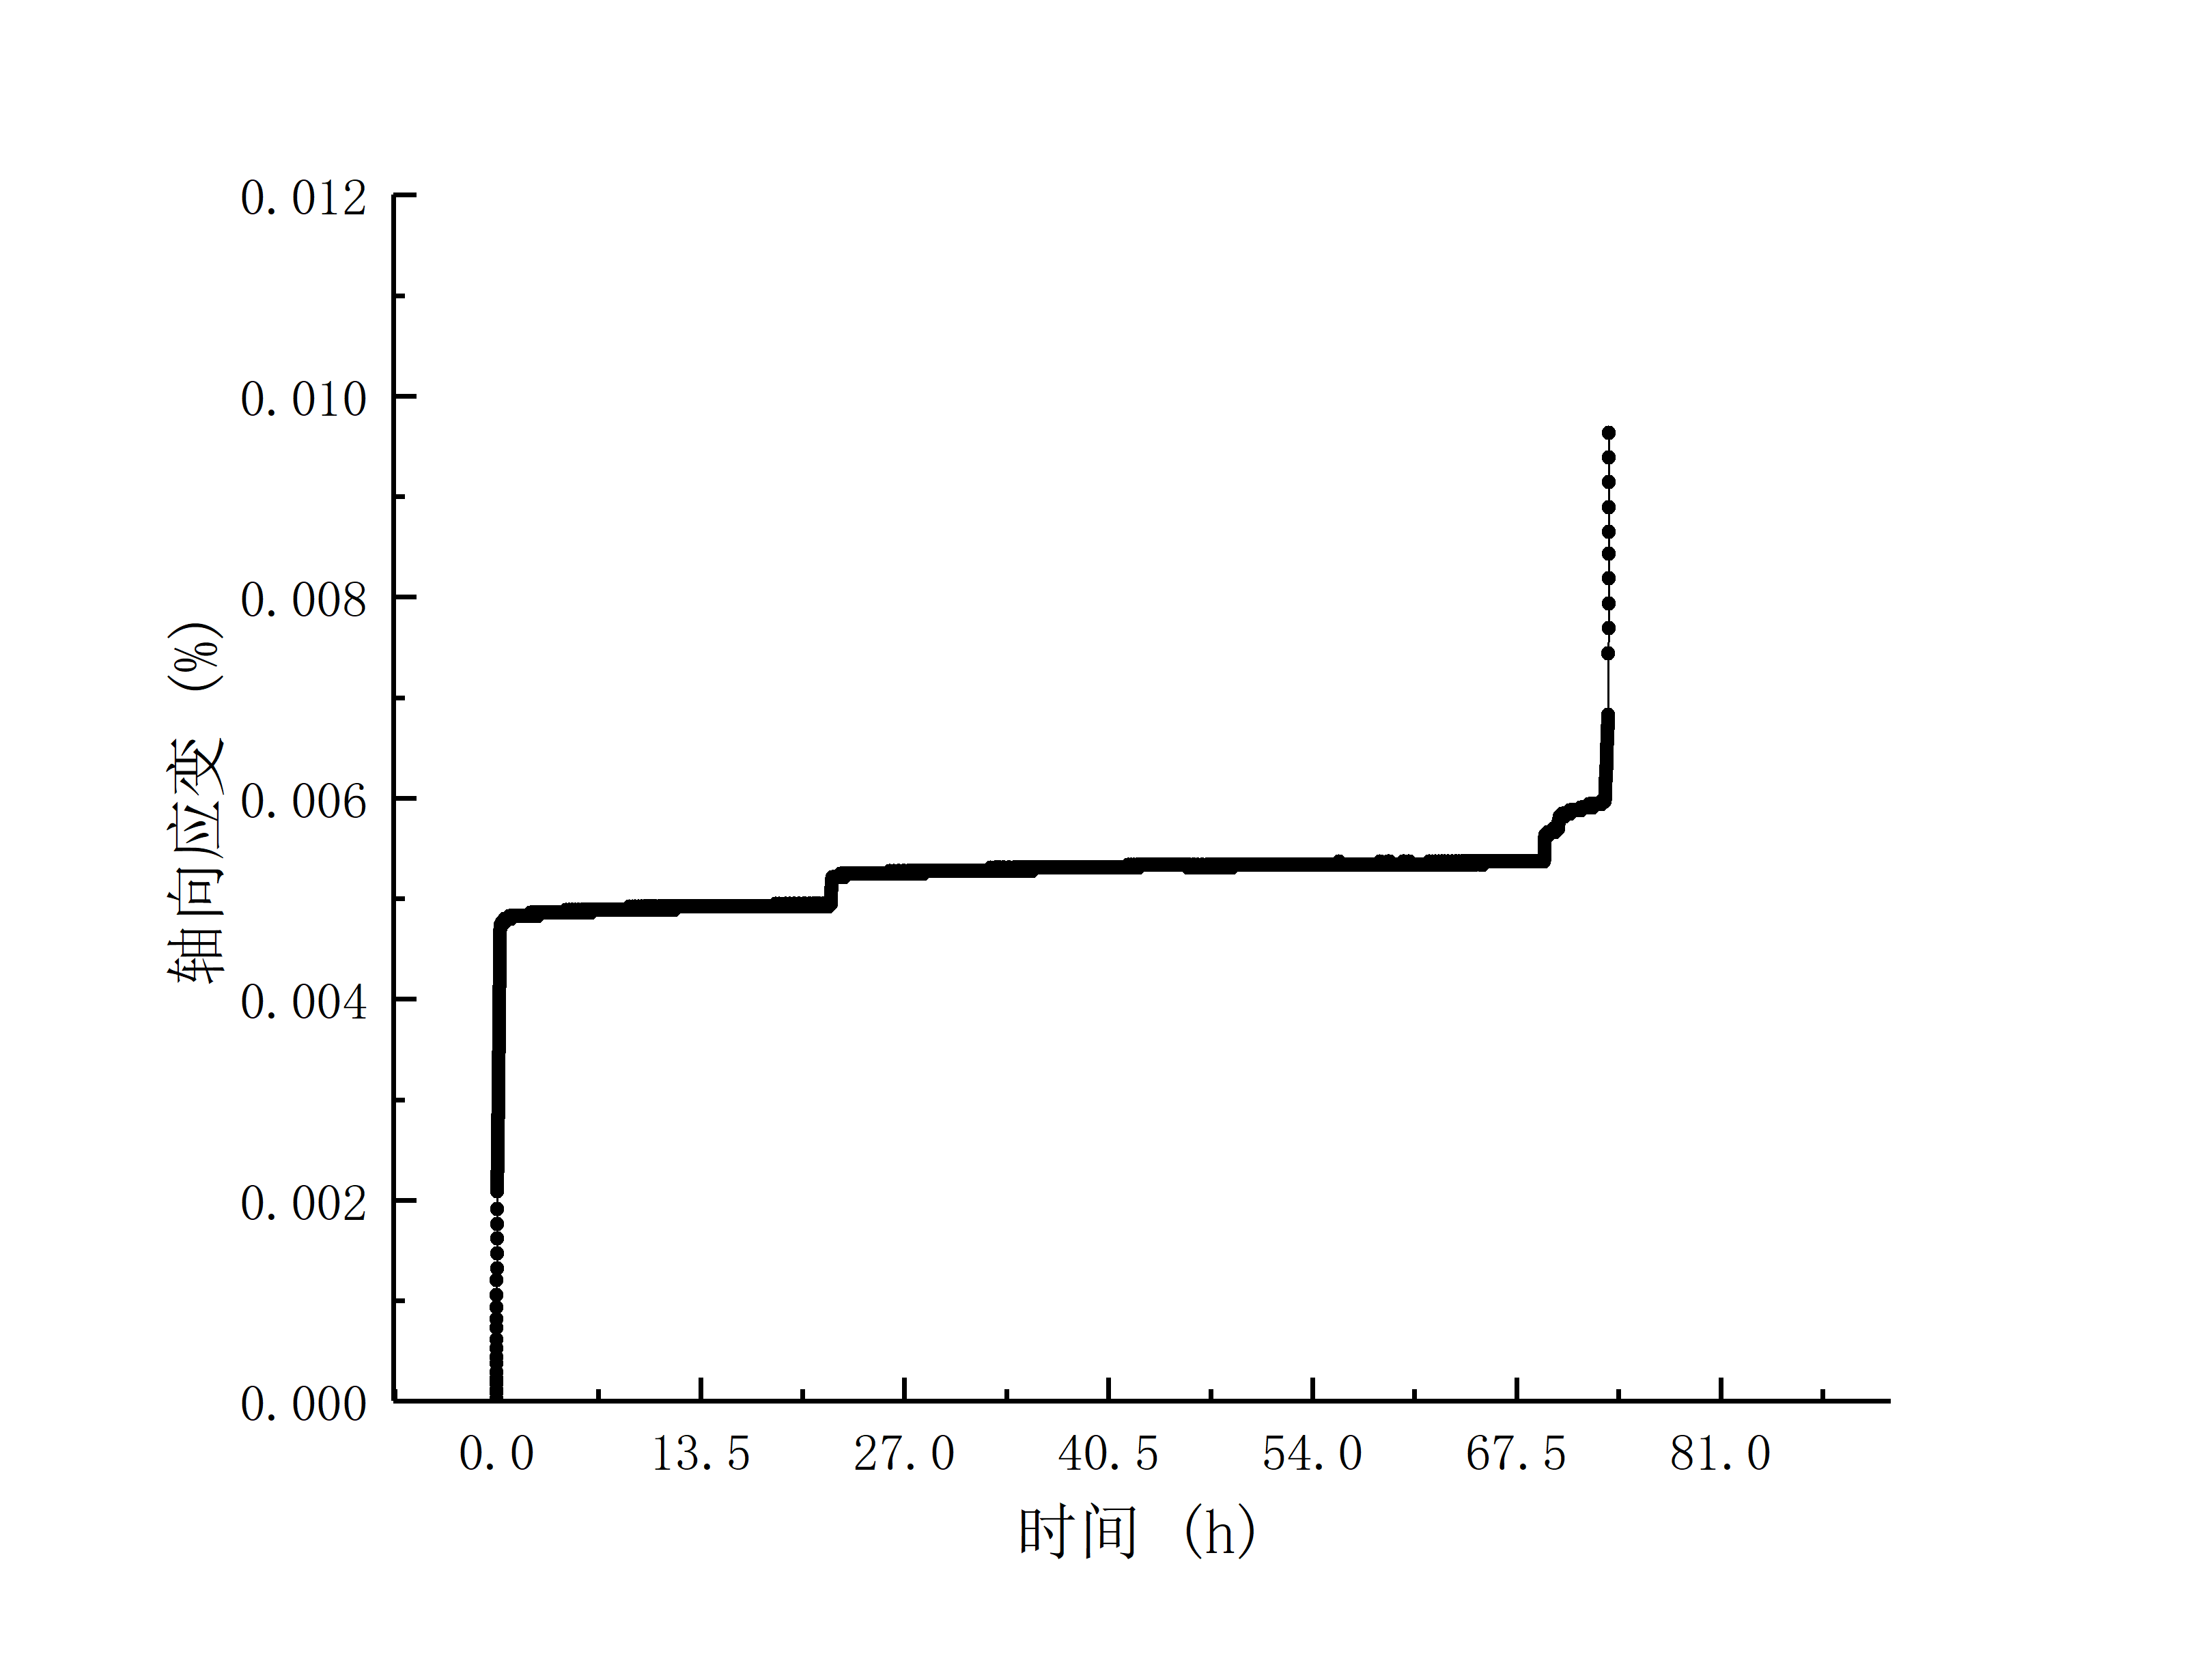
\includegraphics[width=1.2\textwidth]{img/chap2/D-01.png}
        \end{minipage}
    }
    \subfigure[D-02]
    {
        \begin{minipage}{7cm}
            \centering
            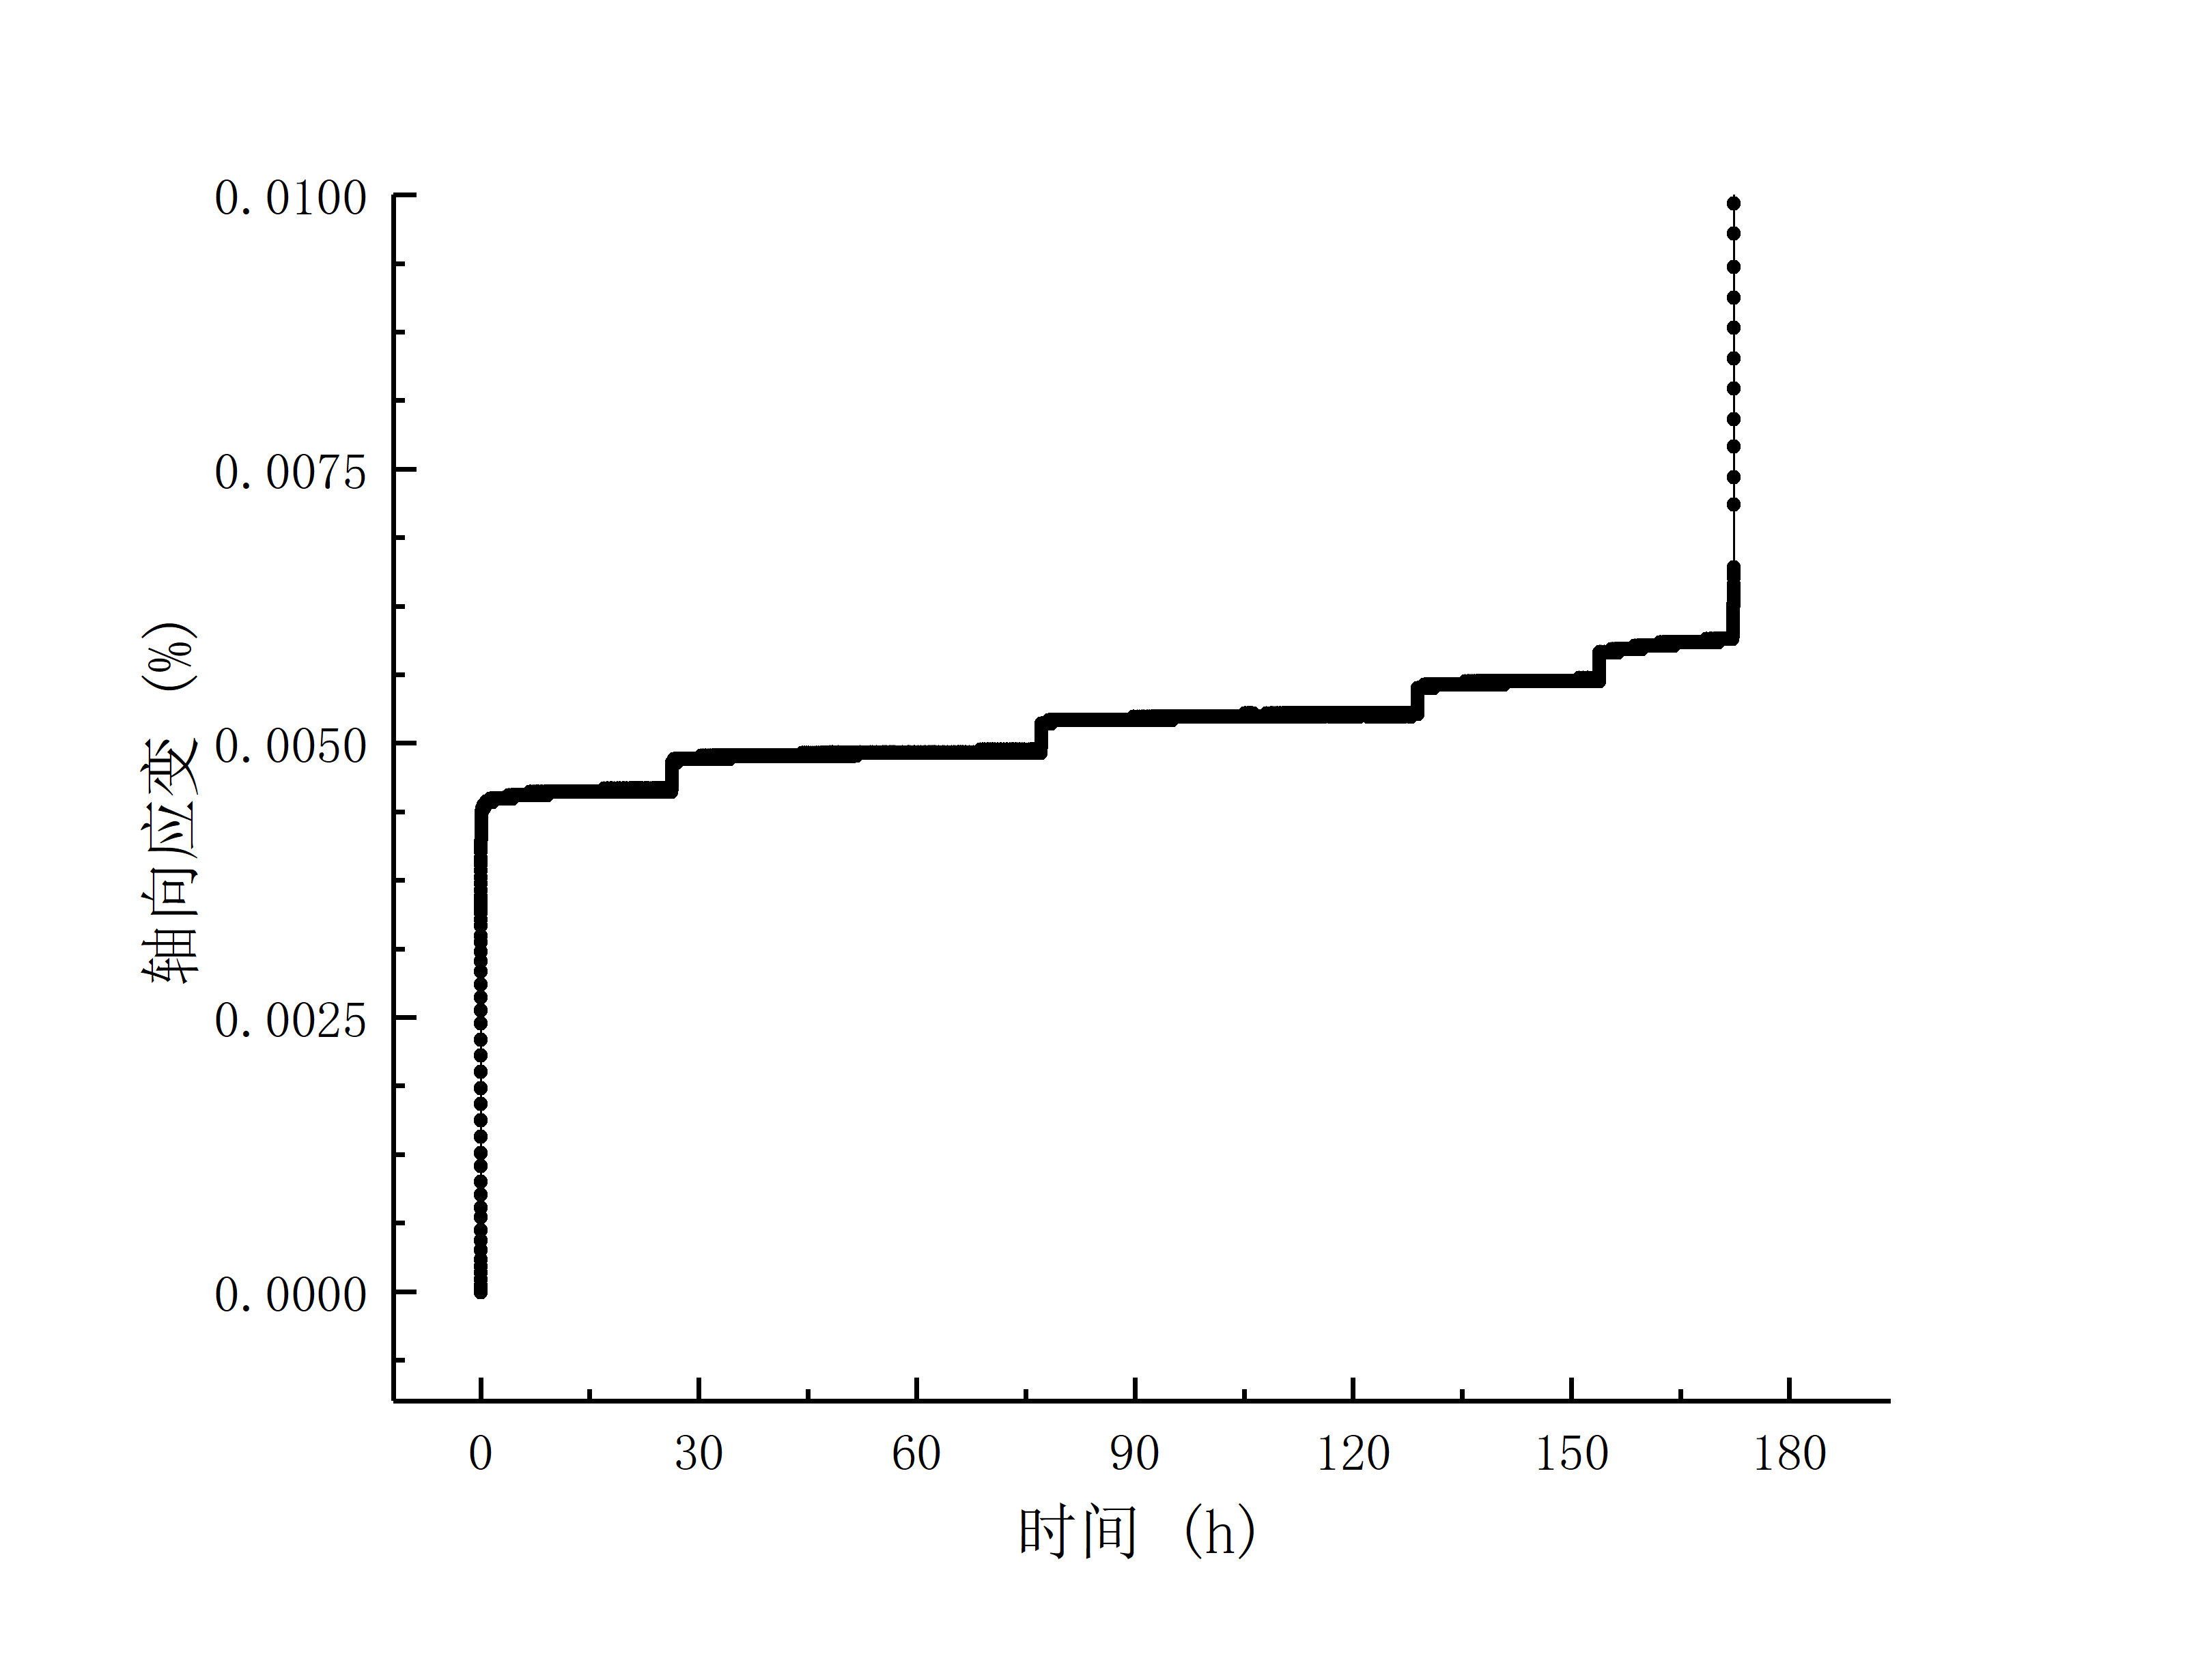
\includegraphics[width=1.2\textwidth]{img/chap2/D-02.png}
        \end{minipage}
    }
	
    \centering
    \subfigure[D-03]
    {
        \begin{minipage}{7cm}
            \centering
            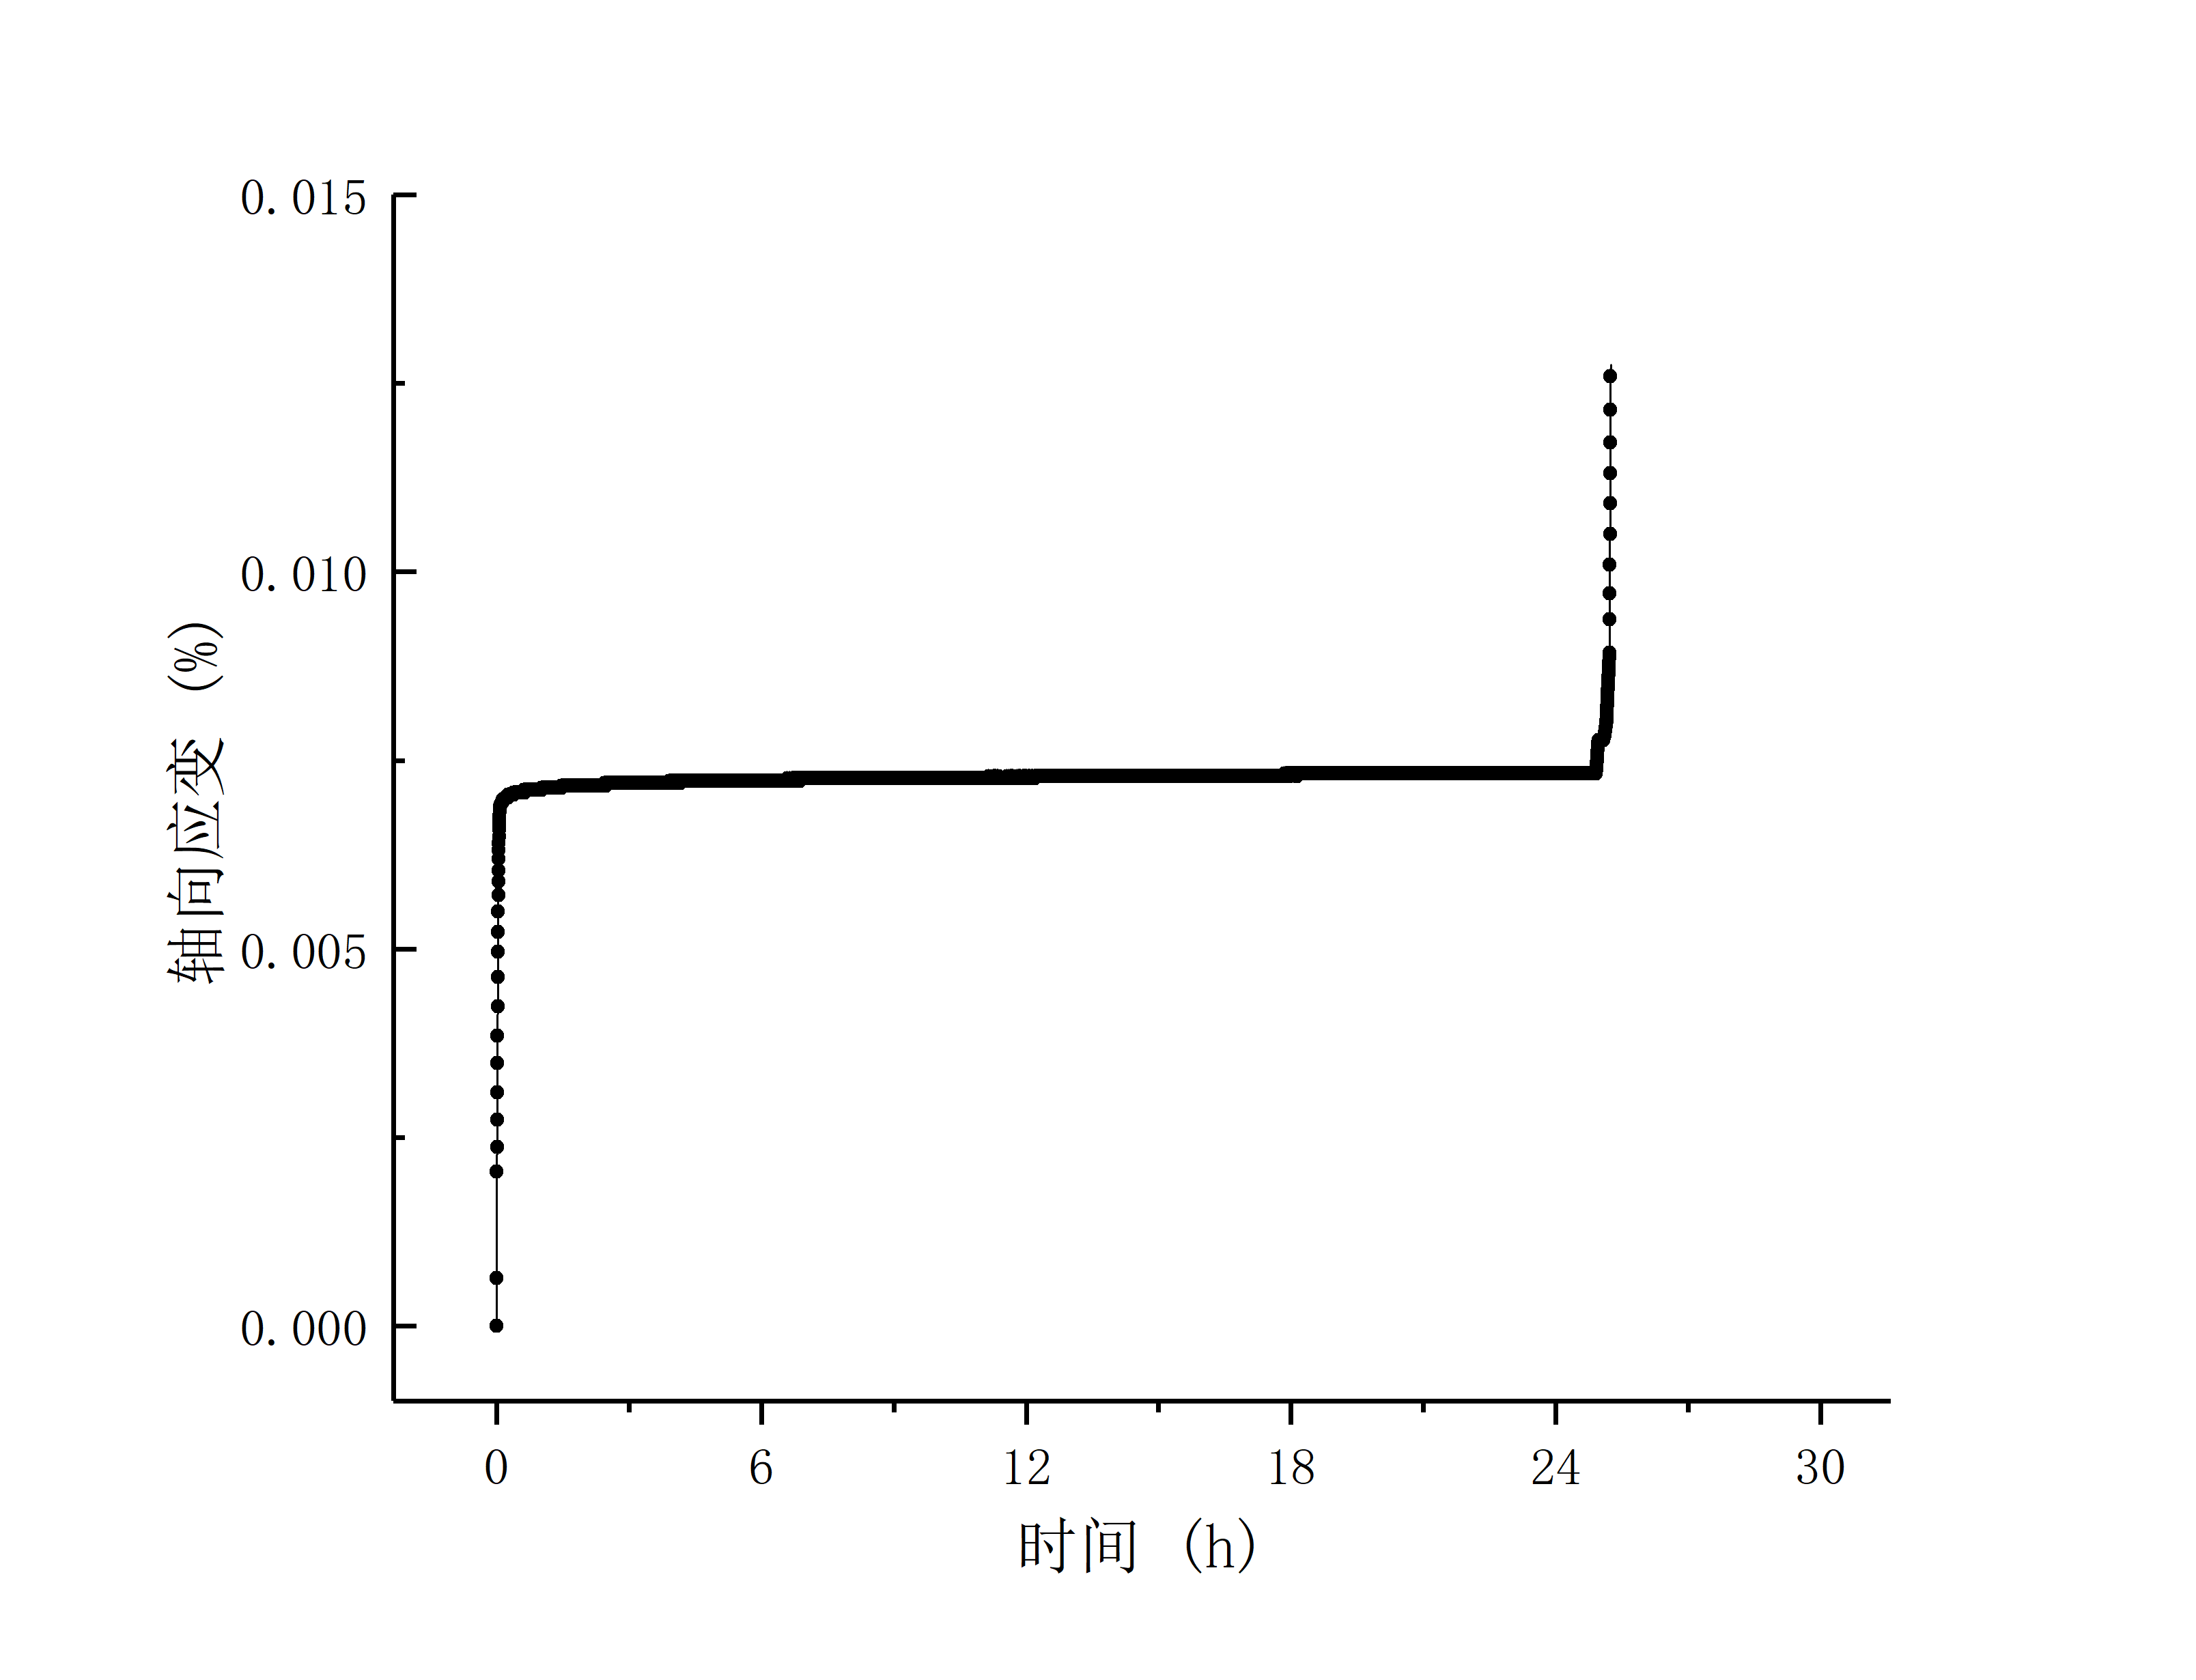
\includegraphics[width=1.2\textwidth]{img/chap2/D-03.png}
        \end{minipage}
    }
    \centering
    \caption{泥岩三轴压缩蠕变试验曲线图}
    \label{fig:2-11}
\end{figure}


\subsection{三轴流变曲线分析}
为了更好地研究泥岩的蠕变特性,更直观地观察泥岩流变曲线的变化趋势,需要将三轴流变试验中采用分级加载法的试样所得到的流变全程曲线(如图~\ref{fig:2-11})转变为一组不同应力加载等级下的分别加载流变曲线,本文采取Boltzmann叠加原理对分级加载曲线进行处理。

为了得到一组不同应力水平下的流变曲线。通常的处理方法是坐标平移法,即把每一级加载的时刻作为该级应力水平下蠕变曲线的起始时刻,而后的时间从该时刻算起,这种做法的依据就是Boltzmann叠加原理,Boltzmann叠加原理是用于线性黏弹性体的处理方法,它是描述不同时间加上不同荷载时材料的变形,该原理指出:对于蠕变过程,各级加载过程对物体变形的贡献是独立的,总的蠕变是各个加载级的蠕变的线性加和。

首先将若干个Kelvin模型串联起来,可以得到被称为广义Kelvin模型的蠕变模型,此模型响应的总应变为各元件应变之和,可以得到蠕变应变表达式如下:

\begin{equation}
     {\varepsilon(t)}={\sigma_0}(\frac{1}{E}+\frac{1}{\eta}t+\int_{0}^{\infty} \frac{1}{E(\tau)}(1-e^{-\frac{1}{\tau}t}) d{\tau})
\end{equation}

记$J_\infty=\frac{1}{E}$ ,$\Psi(t)=\int_{0}^{\infty} \frac{1}{E(\tau)}(1-e^{-\frac{1}{\tau}t}) d{\tau}$

则
\begin{equation}
     {\varepsilon(t)}={\sigma_0}(J_\infty+\frac{1}{\eta}t+\Psi(t))
\end{equation}

上式是由广义Kelvin模型积分的得到蠕变条件下蠕变变形的本构方程式,由此可以得到蠕变柔量,记为$J(t)$

\begin{equation}
J(t)=\frac{\varepsilon(t)}{\sigma_0}
    =J_\infty+\frac{1}{\eta}+\Psi(t)
\end{equation}

所示蠕变积分方程,如果在$\tau=0$时施加荷载$\sigma_0$,就可以得到该时刻的应力-应变关系:

\begin{equation}
{\varepsilon_0(t)}={\sigma_0}{J(t)}
\end{equation}

那么,在$t=\tau_1$时,施加第二个应力增量$\sigma_1$,相应的应变响应为:
\begin{equation}
{\varepsilon_1(t)}={\varepsilon(t-\tau_1)}={\sigma_1}{J(t-\tau_1)}
\end{equation}

如果将这两个应变叠加,则
\begin{equation}
     {\varepsilon(t)}={\sigma_0}{J(t)}+{\sigma_1}{J(t-\tau_1)}
\end{equation}

将该公式推广到一般情况下,在时刻$\tau_1$,$\tau_2$,$\cdots$,$\tau_n$分别施加应力增量$\sigma_1$,$\sigma_2$,$\cdots$,$\sigma_n$,则$\tau_i>0$时的应变总量即为:
\begin{equation}
     {\varepsilon(t)}=\sum_{i=0}^n\varepsilon_i(t)=\sum_{i=0}^n\sigma_iJ(t-\tau_i)
\end{equation}

若从$t_1$时刻起,应力随时间变化连续,即当时间间隔趋于无穷小时,总应变可以用下
列积分形式表达:
\begin{equation}
     {\varepsilon(t)}=\int_{0}^{\infty}J(t-\tau)\frac{\partial\sigma}{\partial\tau}d\tau
     \label{eq:2-9}
\end{equation}

式\ref{eq:2-9}说明在某时刻的变形不仅与该时刻的应力值有关,而且与应力、变形的历史有关。

我们对三轴流变试验得到的阶梯型数据曲线进行坐标平移,将每个阶段的加载过程起始点都平移至零点处,得到的曲线图如下图\ref{fig:2-10}所示。
\begin{figure}[ht!]
    \centering
    \subfigure[D-01]
    {
        \begin{minipage}{7cm}
            \centering
            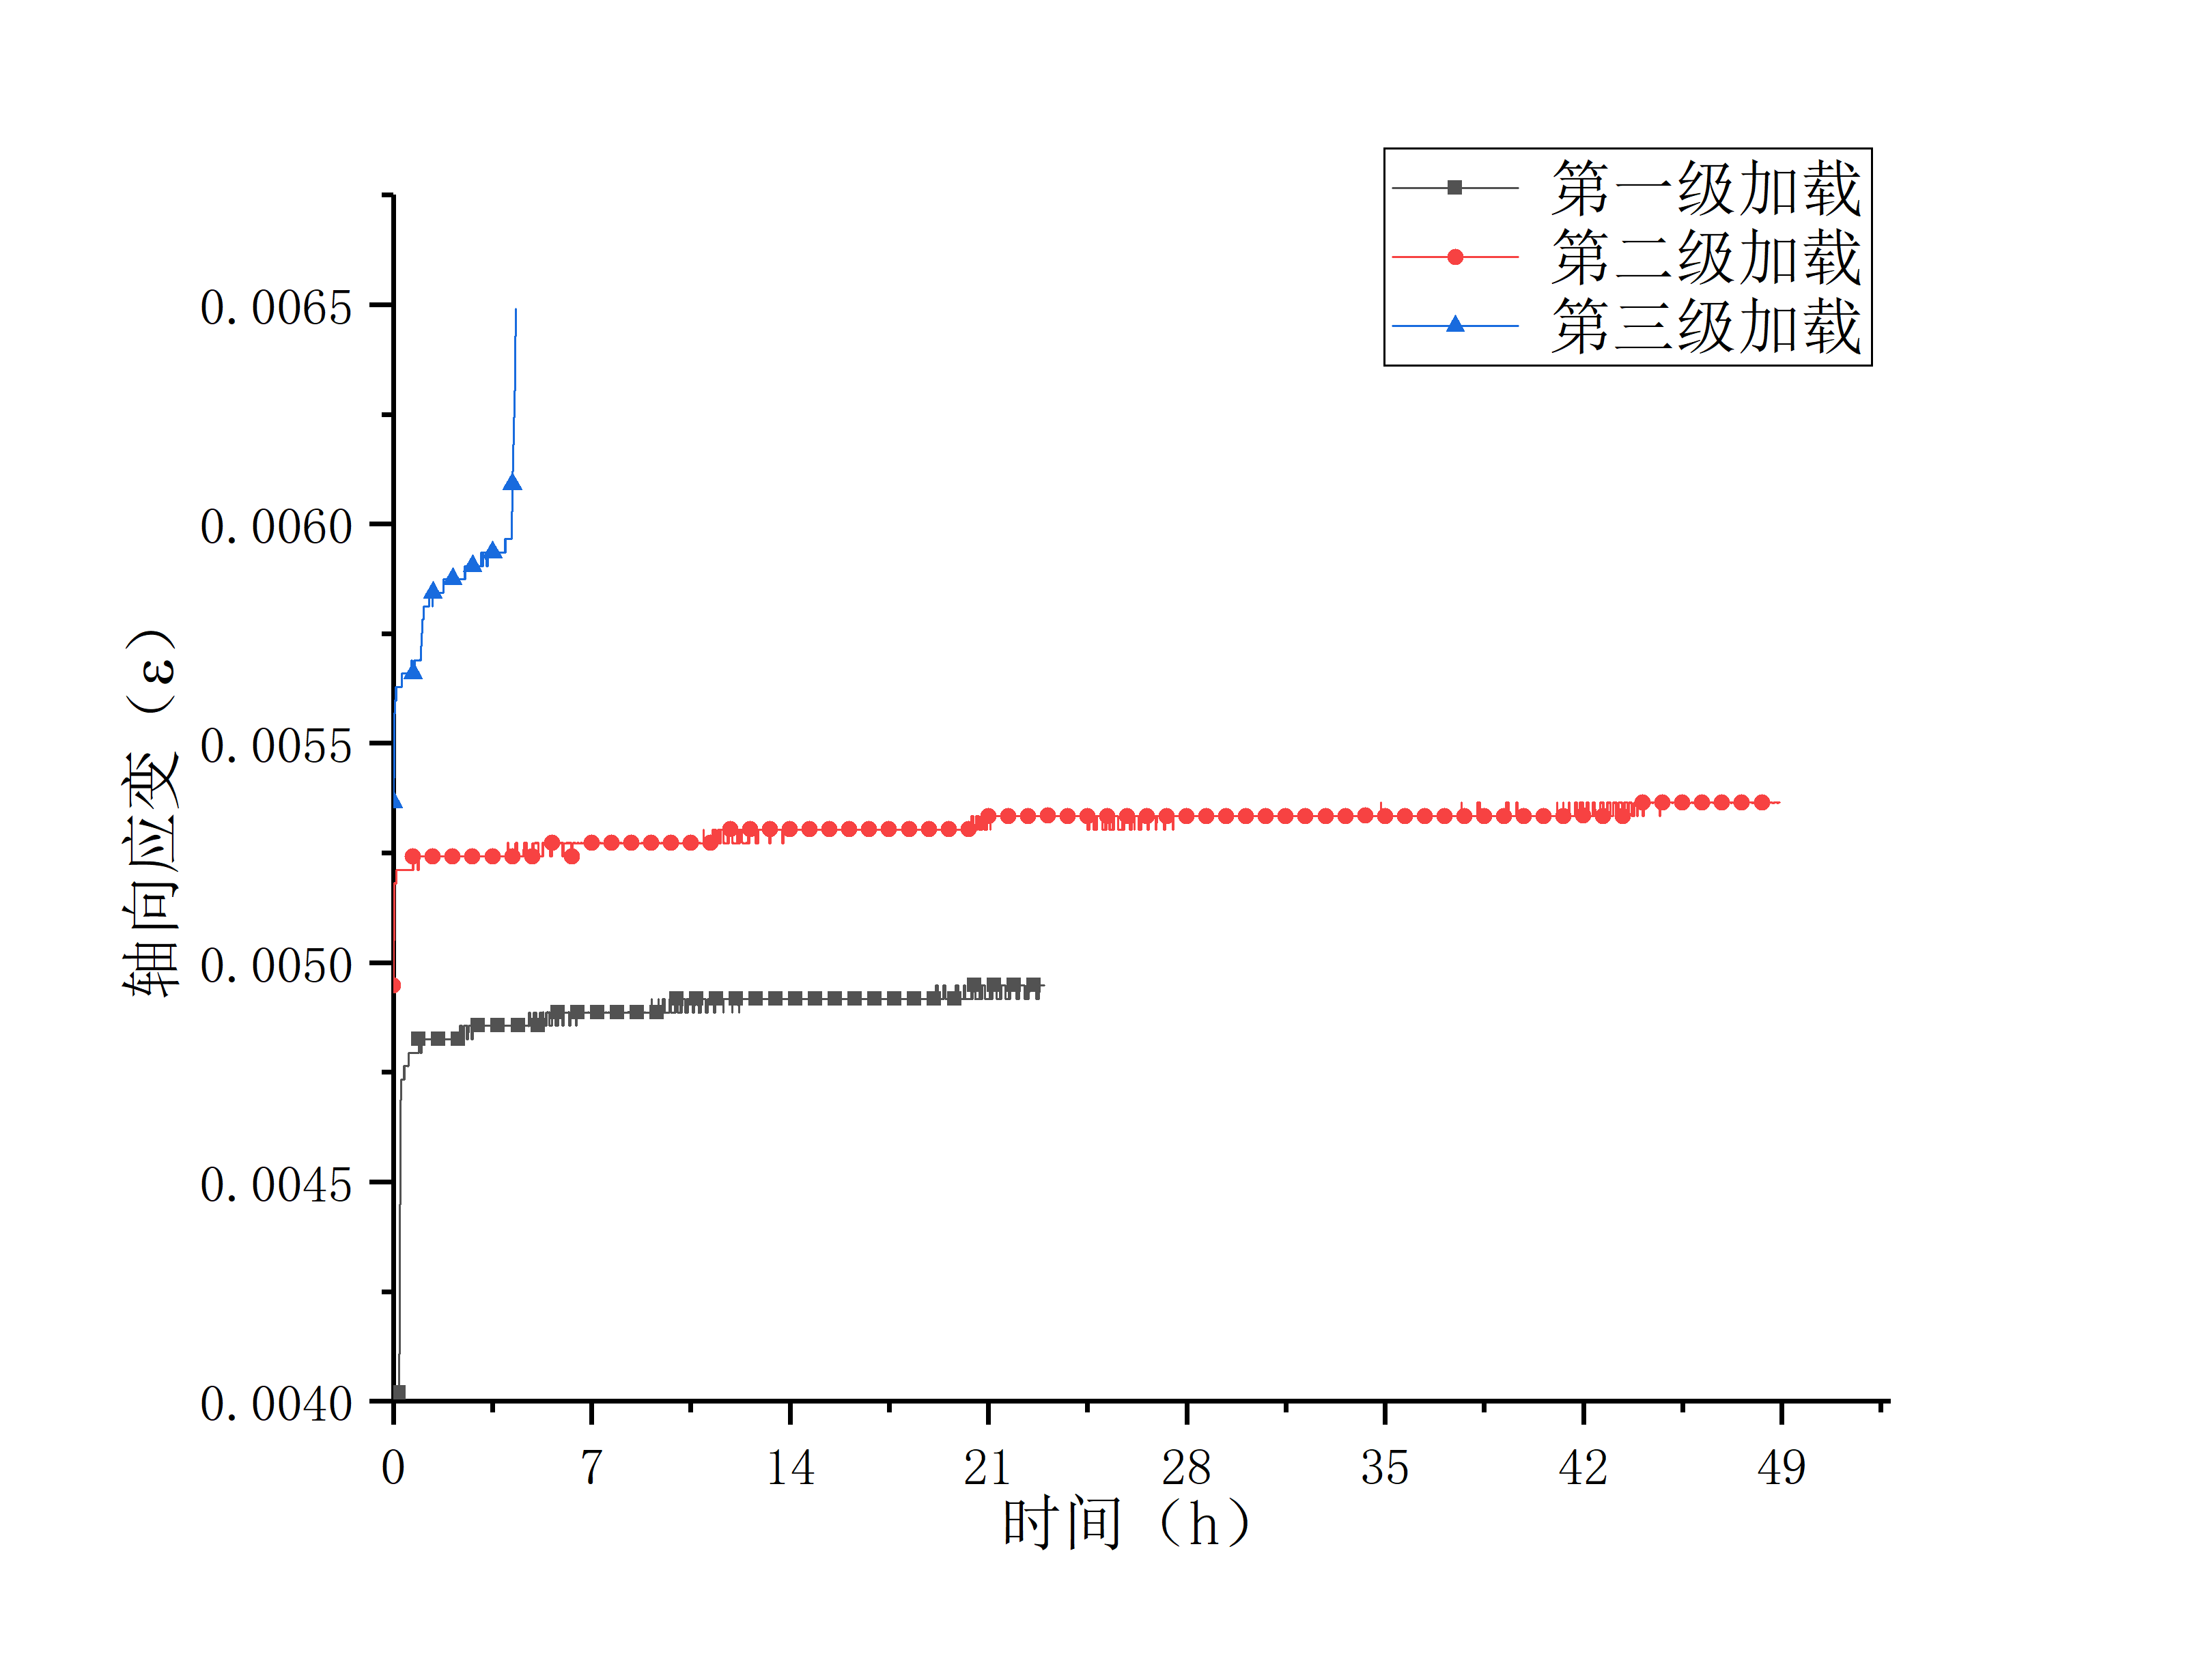
\includegraphics[width=1.2\textwidth]{img/chap2/D-01-B.png}
        \end{minipage}
    }
    \subfigure[D-02]
    {
        \begin{minipage}{7cm}
            \centering
            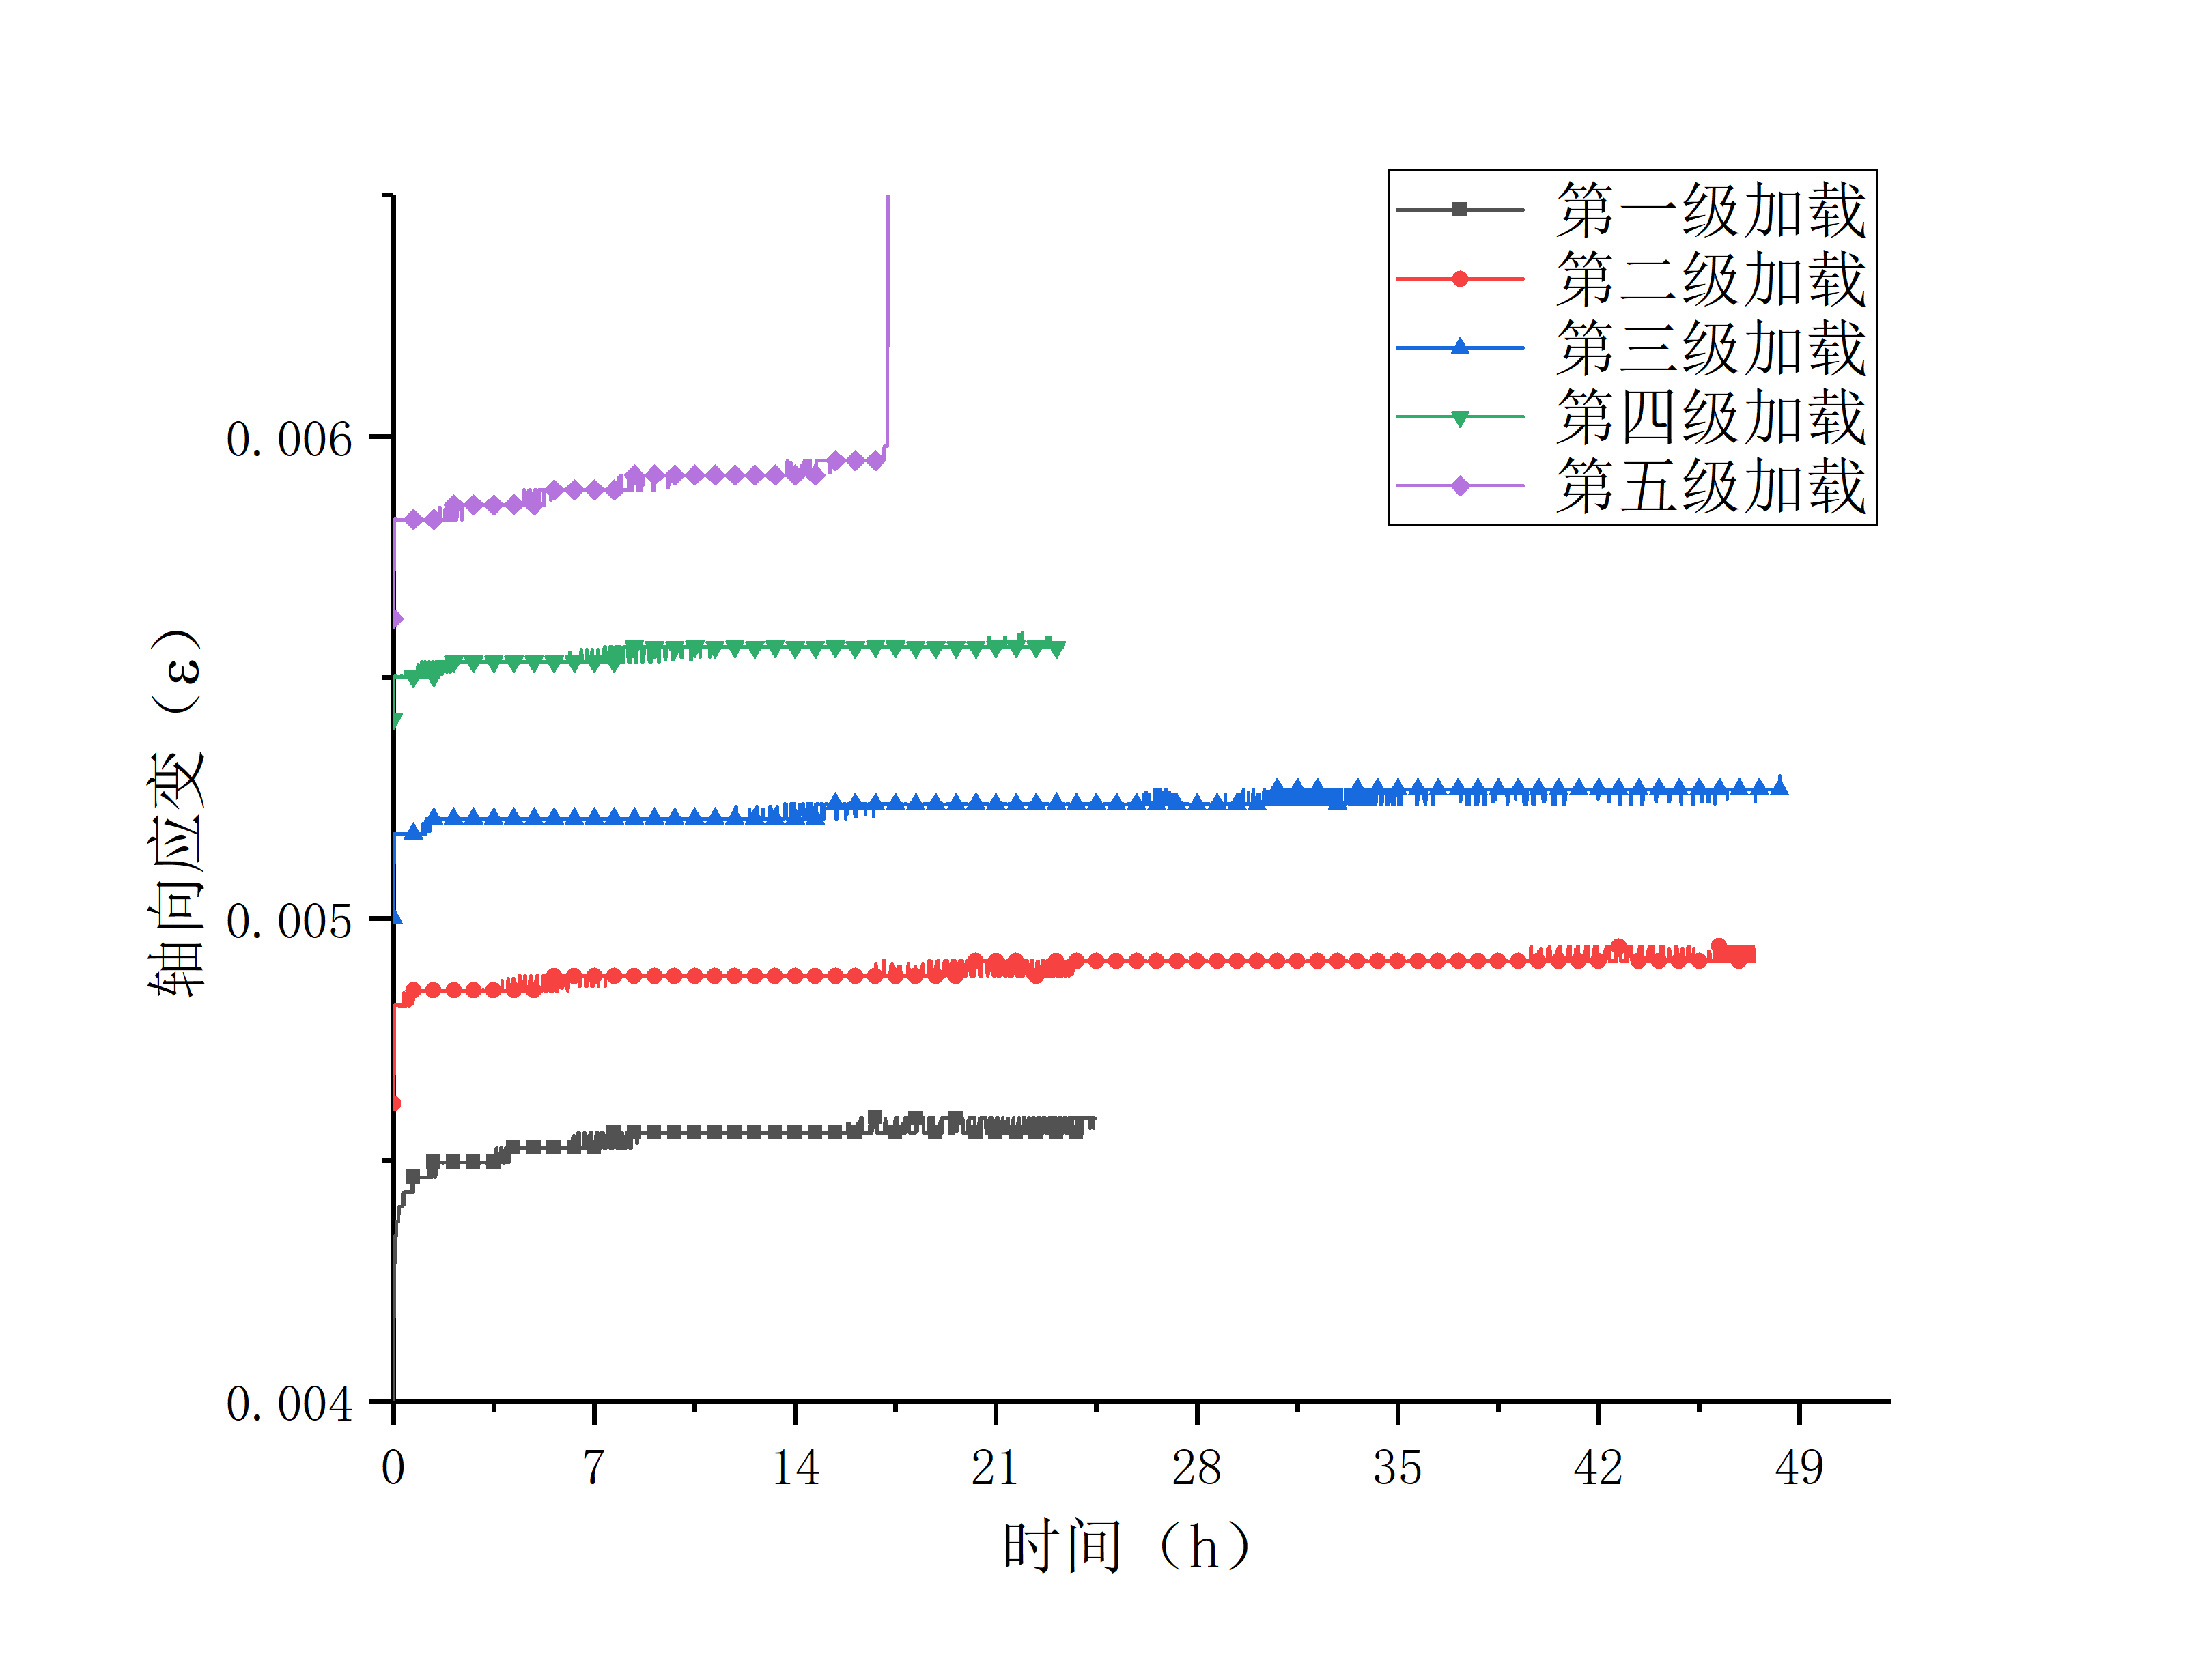
\includegraphics[width=1.2\textwidth]{img/chap2/D-02-B.png}
        \end{minipage}
    }
	
    \centering
    \subfigure[D-03]
    {
        \begin{minipage}{7cm}
            \centering
            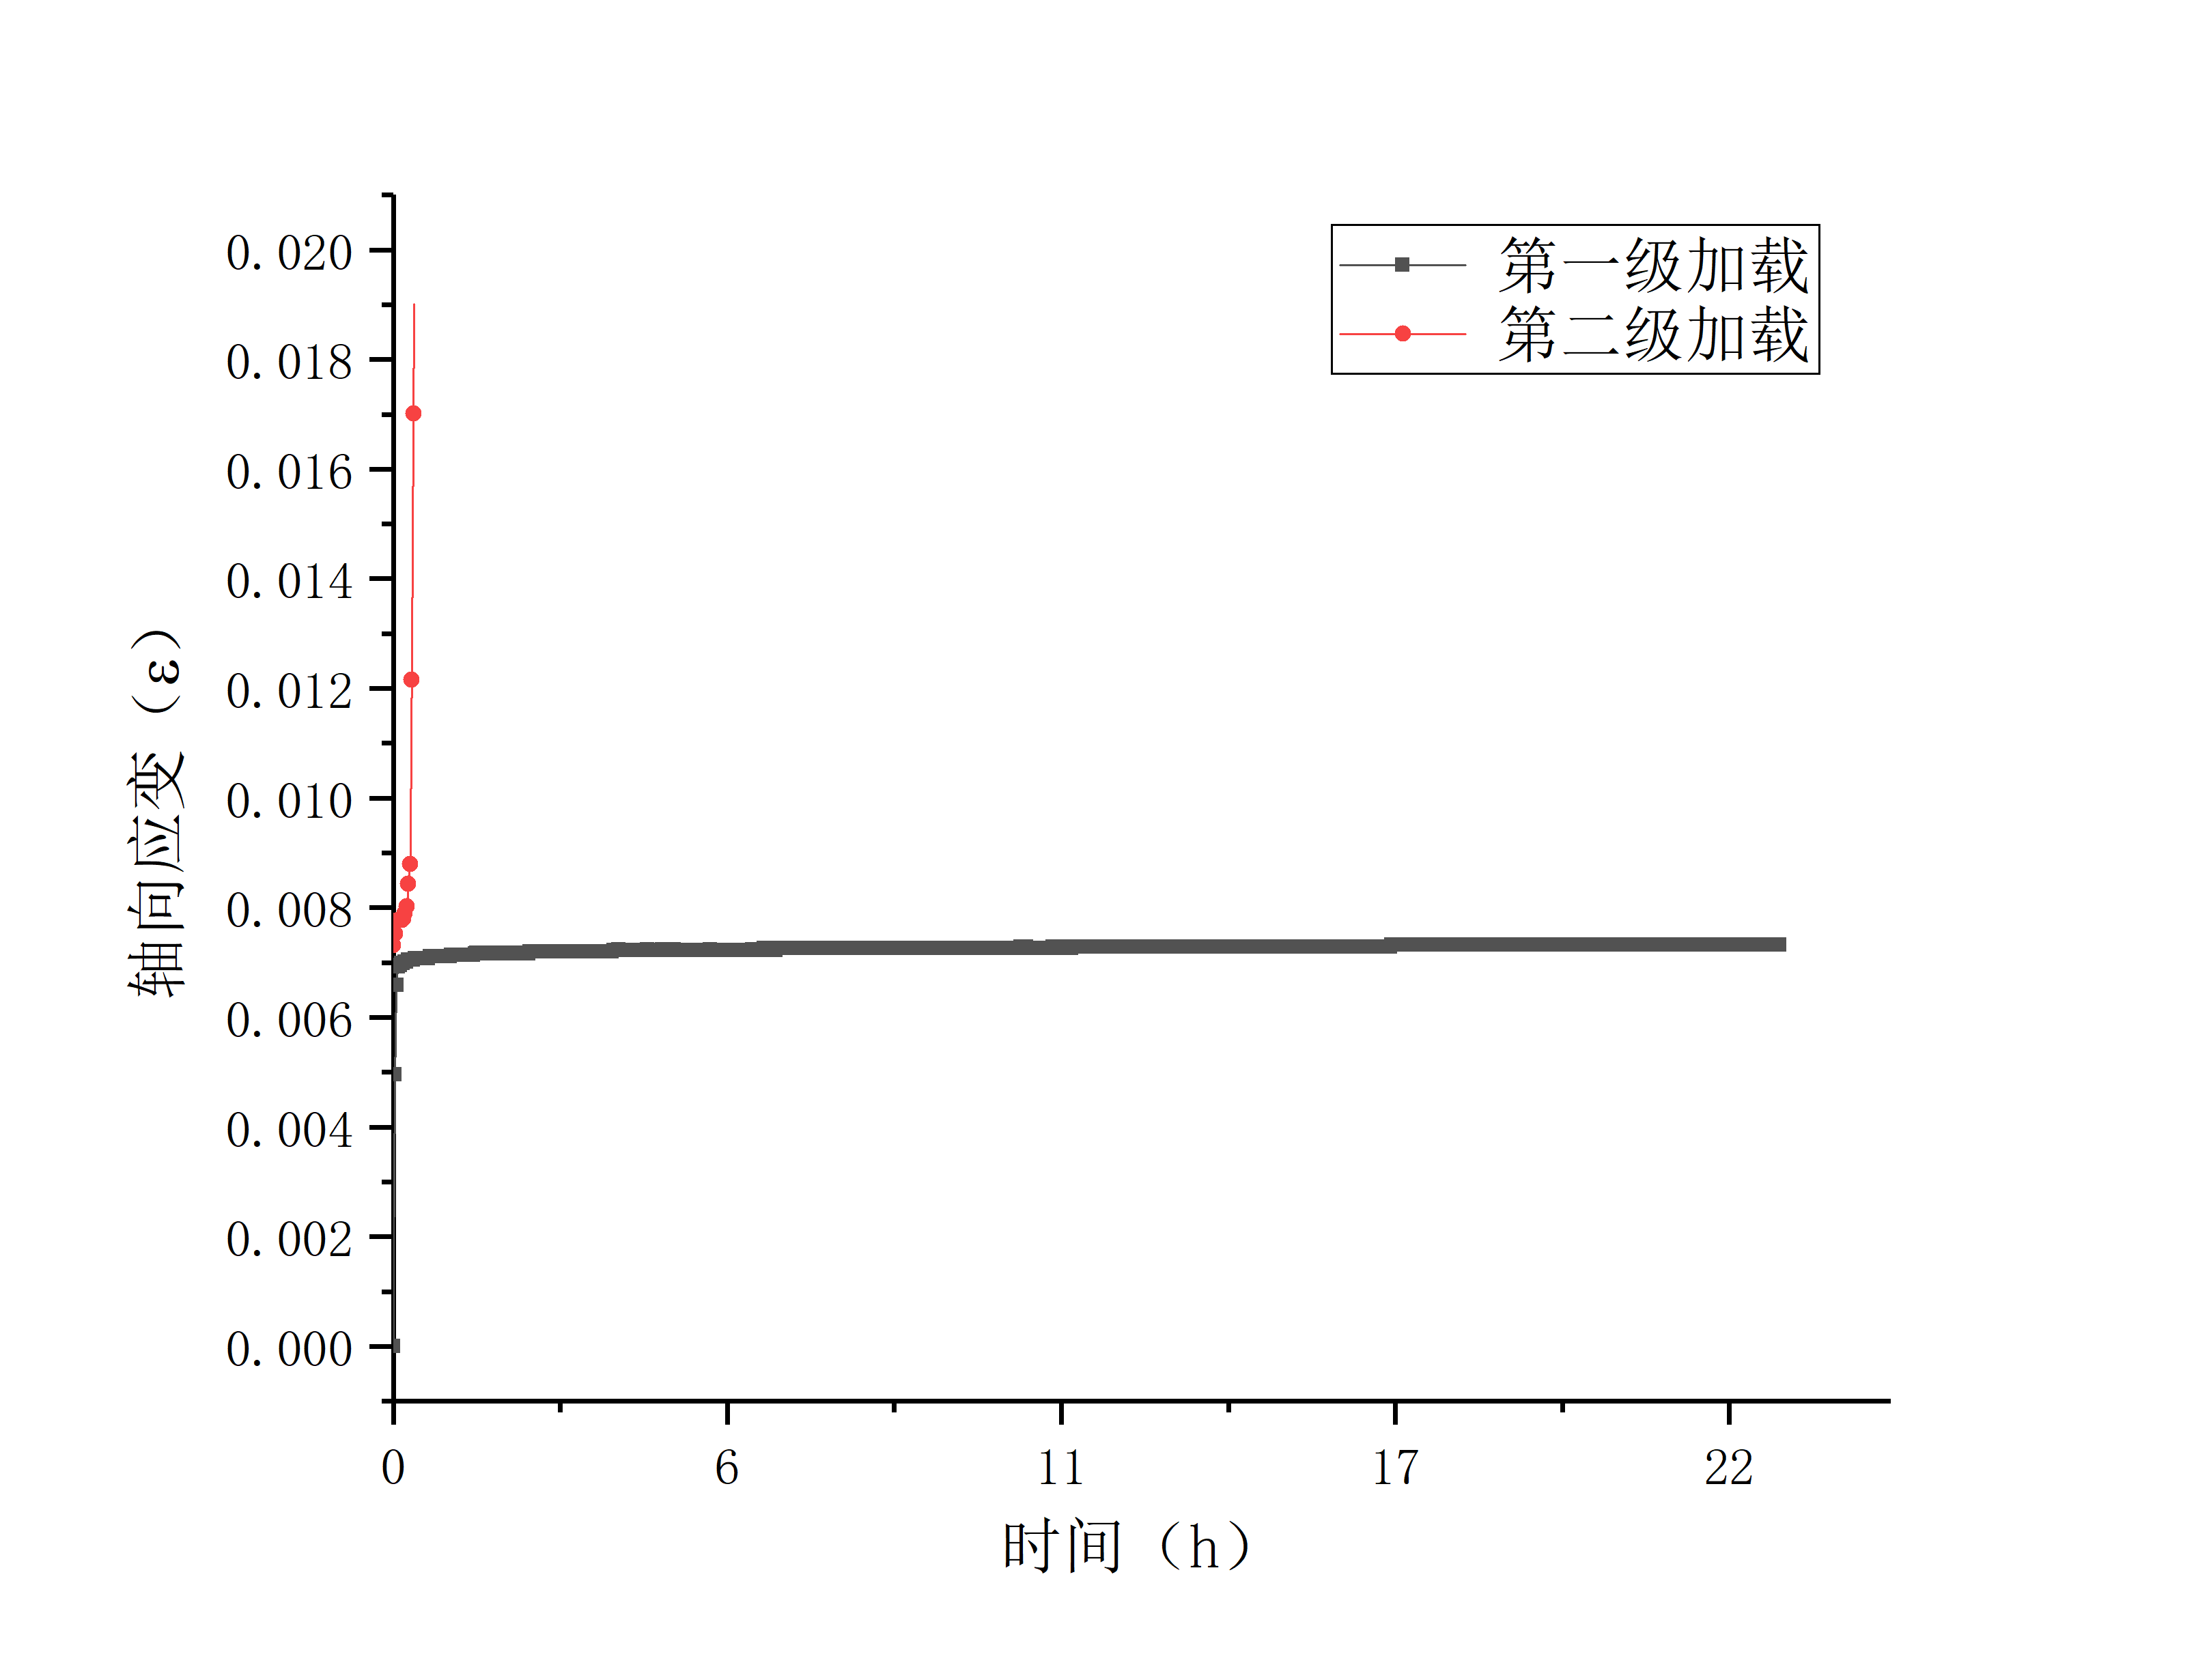
\includegraphics[width=1.2\textwidth]{img/chap2/D-03-B.png}
        \end{minipage}
    }
    \centering
    \caption{泥岩流变试验同围压下各级加载曲线图}
    \label{fig:2-12}
\end{figure}

考虑在同一围压下不同加载等级下的流变曲线,由图\ref{fig:2-12}可知:

(1)在同一围压下的泥岩试样流变曲线中,试样在加载的瞬间都会产生瞬时变形,不过由于本次采用的是分级加载的方式,而不是分级加卸载的试验形式,因此从第二级架子开始的瞬时轴向应变普遍较小。随着应力等级的提升,试样的流变速率也随之增大,说明应力水平越高,泥岩试样的流变特性越明显。

(2)在较低的应力等级下,岩石以瞬时变形为主,流变变形量较小。例如,在\SI{10}{MPa}的围压下,第一级应力加载时,达到稳定蠕变阶段时,瞬时轴向应增加了0.0045,而在之后的流变阶段,仅产生了0.00009的轴向应变;而在第五级应力的加载下,则产生了0.00015的瞬时应变和0.00015的流变应变,随着加载应力的提升,流变变形比重逐渐增大。

(3)在流变过程中,在较低的应力等级下,岩石以瞬时变形为主,流变变形量较小,在经历一定时间后流变变形量收敛,趋于定值,流变变形速率减小到无限趋近于零,在经过一段时间后,试样应变不再增加,趋于一个稳定的值;而当应力等级较高时,在经历一定时间后,流变变形速率趋于某一不为零的定值,流变速率保持不变,试样轴向应变随着时间呈线性增长,这一点从图 2.9(b) 中可以较为清楚的看到。

(4)泥岩试样的三轴流变试验结果表明,该泥岩具有较为显著的流变特性,且在流变过程中,较长时间都处于稳定蠕变阶段。不过,在本次进行的三组三轴流变试验都没有完成预期的加载目标,D-01完成了两组加载等级,在第三级加载时试样就已经破坏,D-03则是只完成了一组加载,第二级加载开始后试样便迅速破坏了,仅有第二组D-02加载到了第五级,综合常规三轴压缩试验的结果,这主要是由于试样强度不够均匀,通过压缩试验选取的应力加载水平过大。

(5)在流变曲线中,我们发现应变在某些阶段会上下波动,这与单轴流变试验的曲线波动原因是一致的,都是因为试样内部存在的微小裂缝对试验数据造成的一些可以忽略不计的影响。


\subsection{加速流变阶段分析}
在三轴流变试验中我们发现了一个在单轴流变试验中未曾出现过的流变阶段——加速流变阶段。在分级加载的最后一级应力水平下,岩石流变变形表现出与以往应力水平不同的时效特征。三轴流变过程中最后一级加载下流变变形及流变速率如图\ref{fig:2-11}所示。

\begin{figure}[ht!]
    \centering
    \subfigure[D-01]
    {
        \begin{minipage}{7cm}
            \centering
            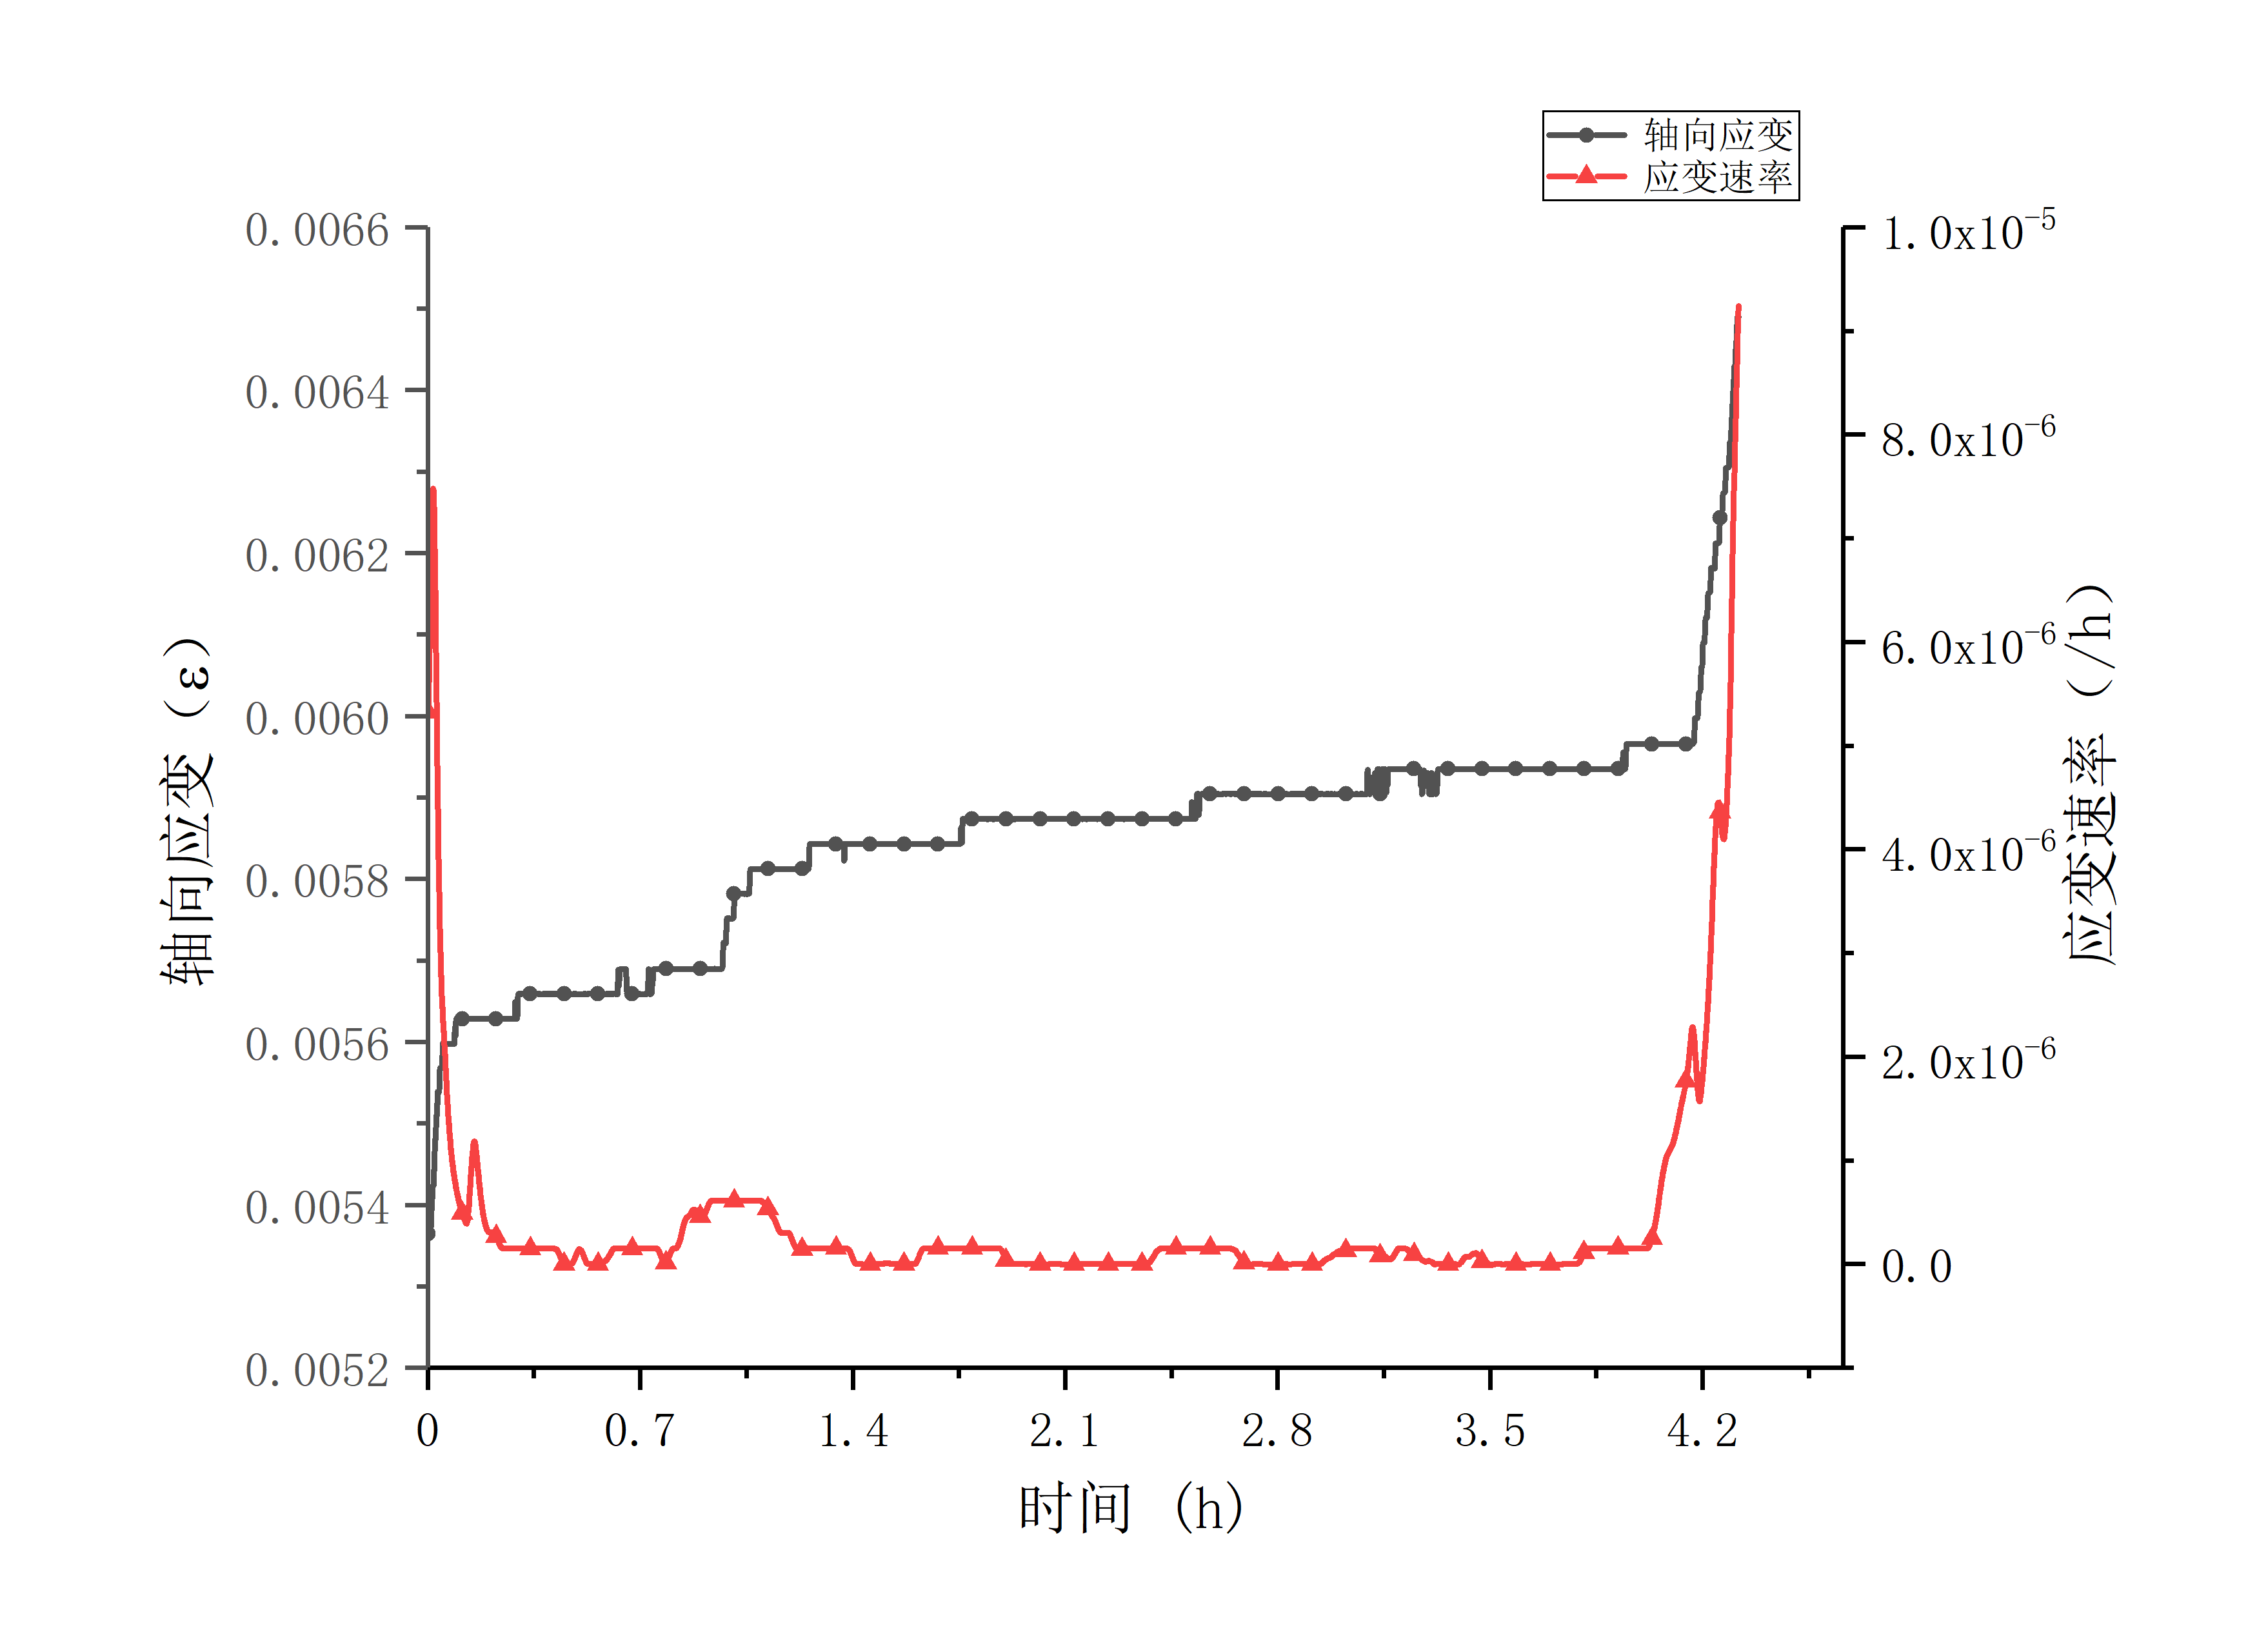
\includegraphics[width=1.2\textwidth]{img/chap2/D-01-v.png}
        \end{minipage}
    }
    \subfigure[D-02]
    {
        \begin{minipage}{7cm}
            \centering
            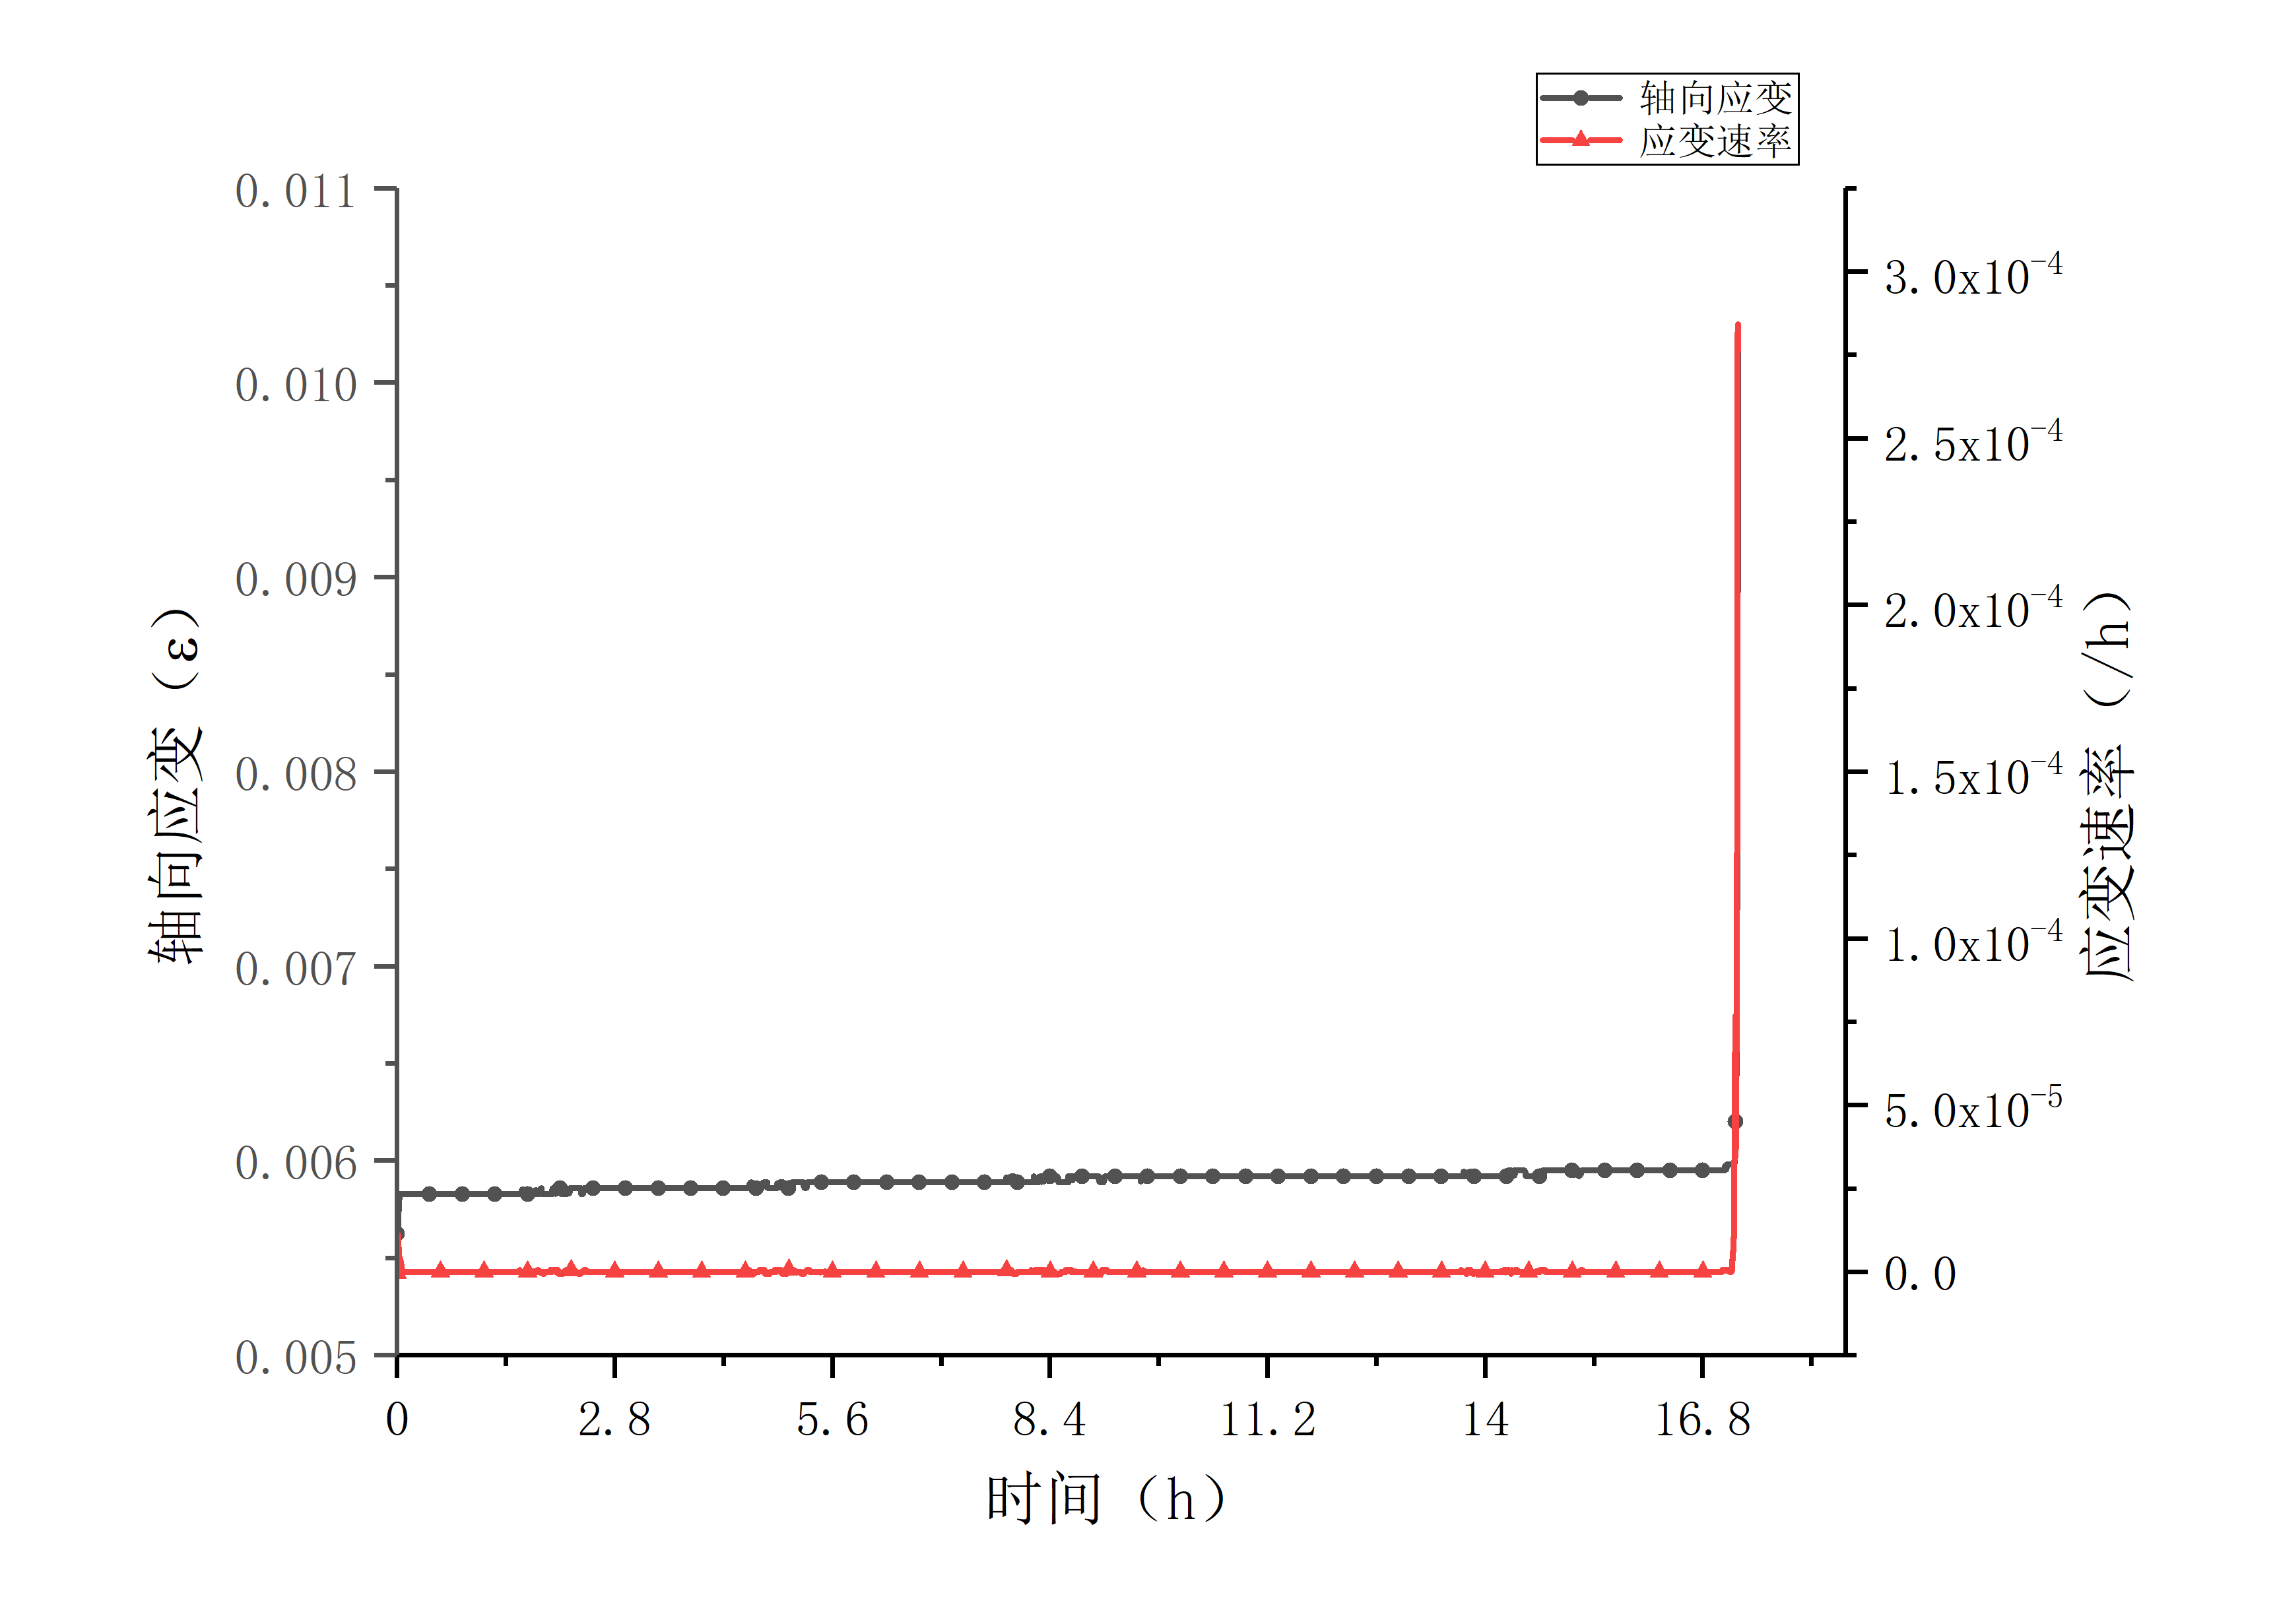
\includegraphics[width=1.2\textwidth]{img/chap2/D-02-v.png}
        \end{minipage}
    }
	
    \centering
    \subfigure[D-03]
    {
        \begin{minipage}{7cm}
            \centering
            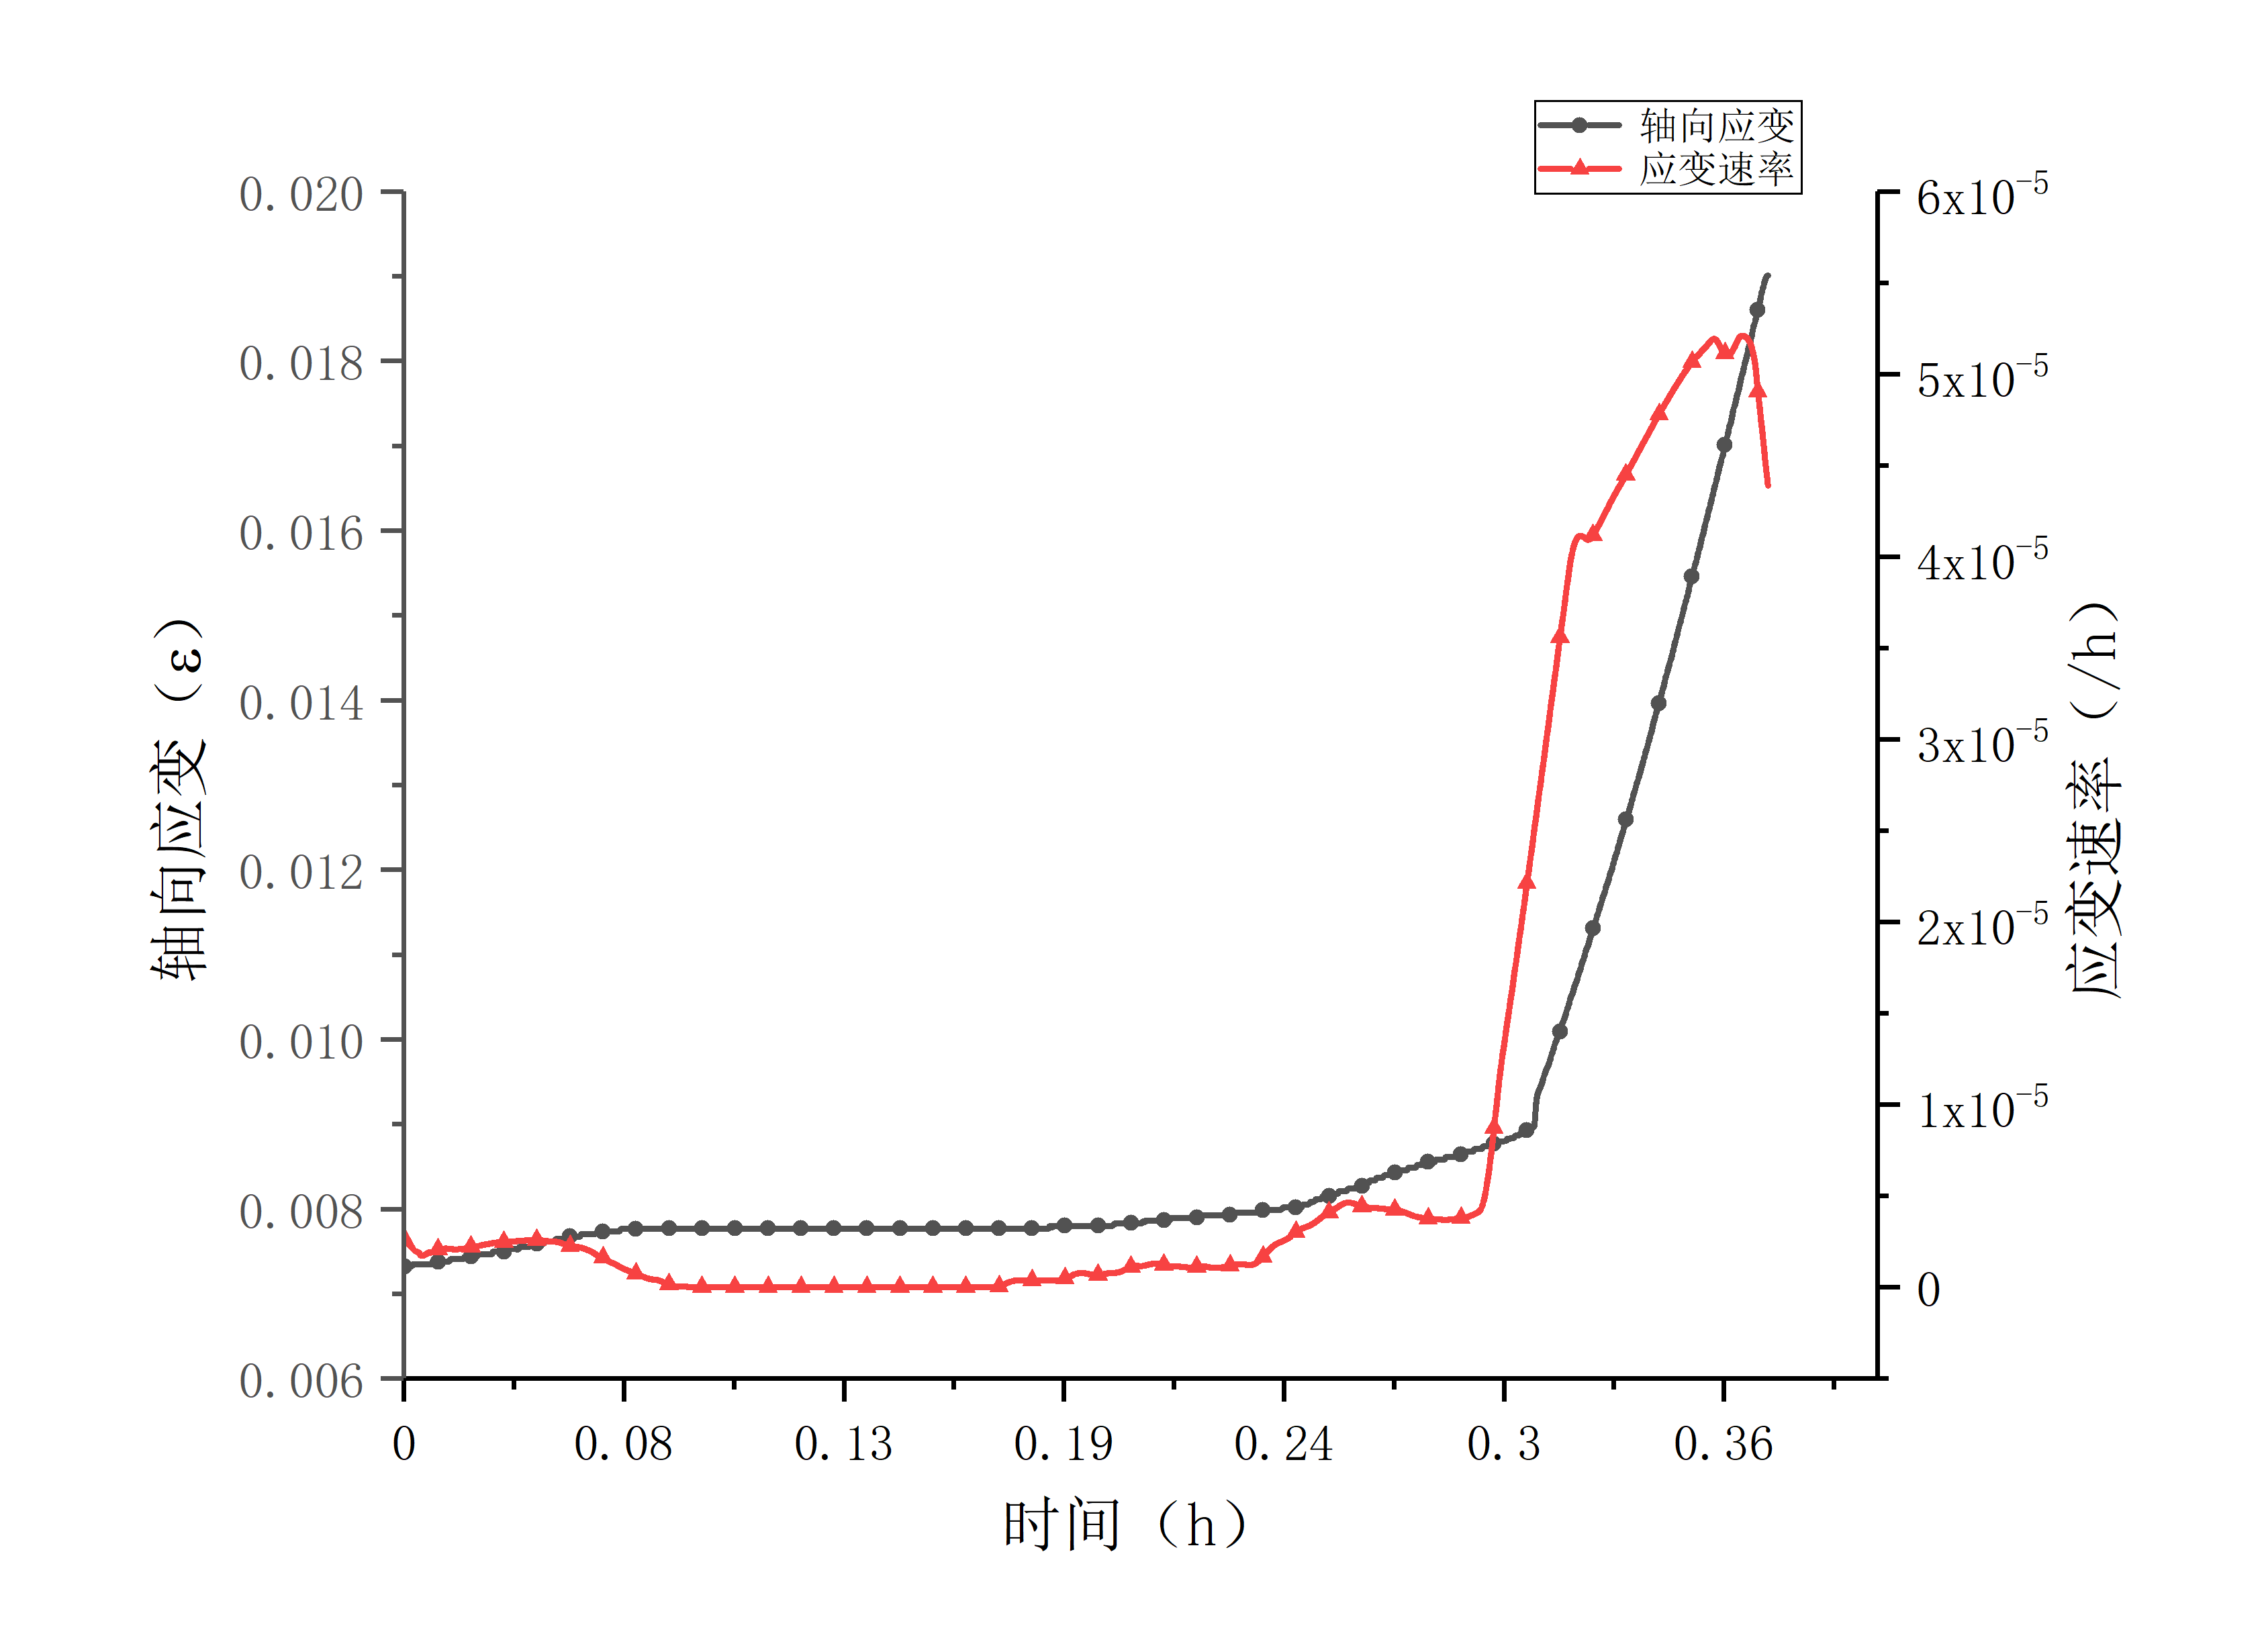
\includegraphics[width=1.2\textwidth]{img/chap2/D-03-v.png}
        \end{minipage}
    }
    \centering
    \caption{加速流变阶段曲线}
    \label{fig:2-13}
\end{figure}

在表示D-03试验的图(c)中,试样仅经历了一小段时间的稳定蠕变,在最后一级加载开始\SI{0.3}{h}后试样就进入了加速蠕变阶段,结合该组试验的数据,研究表明了D-03试样在最后一级加载刚开始时试样就发生了破坏,可以认为在第一阶段的加载过程中岩样已经积累大量损伤,在第二级应力施加仅仅不到20分钟就发生破裂,这主要是因为预期施加的应力过大,超过了泥岩试样的长期强度,导致了试样快速破裂,在此不作为流变破坏探讨。

除D-03以外的两组试验,根据图\ref{fig:2-13}中的(a)、(b)可以发现,试样在最后一级应力加载过程中均经历了衰减蠕变,稳定蠕变和加速蠕变三阶段。泥岩试样流变速率在衰减蠕变阶段逐渐减小,进入稳定蠕变阶段趋于某一较低值。在加速流变阶段,试样的轴向应变突然迅速增加,与此同时,应变速率在同一点处也由稳定的较低值迅速增大,根据记载的数据,轴向应力也迅速减小,从宏观上可以观察到,此时试样出现大量裂缝,试样破坏。
D-01的流变曲线较为光滑,表现为渐进性加速破坏,属韧性破坏,其流变破坏可预见性较高;D-02的流变曲线呈突变性增长,突变起点对应流变速率变化的尖点,反映硬脆性岩石流变破裂特点,其流变破坏可预见性较低。

加速流变阶段尽管只占据流变试验较短的时间,但该阶段流变量却占据流变变形量的主要部分。最后一级应力下试样在不同蠕变阶段历时及流变变形量如表\ref{tab:最后一级应力下试样流变参数}所示。
\begin{table}[H]
\centering
\begin{tabular}{ccccc}%四个c代表有四列且内容居中
\toprule%第一道横线
\multirow{2}{*}{试样编号}&\multicolumn{2}{c}{\textbf{\underline{衰减、稳定蠕变阶段}}}& \multicolumn{2}{c}{\textbf{\underline{加速蠕变阶段}}}  \\
&时间/h & 应变/$\mu\varepsilon$ & 时间/h & 应变/$\mu\varepsilon$ \\
\midrule%第二道横线 
D-01  &4.8&550& 0.4 & 560 \\%Data1跨两行,自动表格宽度
\midrule%第三道横线 
D-02&16.86&330&0.4&4250 \\
\midrule
D-03&0.3&1580& 0.006&10100 \\
\bottomrule%第四道横线
\end{tabular}
\caption{最后一级应力下试样流变参数}
\label{tab:最后一级应力下试样流变参数}
\end{table}



\section{流变对应力—应变曲线的影响}

岩石试样单轴流变作用对应力-应变曲线的影响如图\ref{fig:2-14}所示,与x轴近似平行的曲线部分即代表流变变形。
在应力等级较低时,岩石流变变形量较小,随着应力等级提高,
流变变形显著,这与流变变形与时间的规律完全吻合。与单轴压缩试验下应
力一应变曲线相比,流变作用下的应力一应变曲线也反映了孔隙裂隙压密阶段、弹性
变形阶段、微破裂发展阶段这三个阶段,不过在本次试验中,只有C-03试样最终发生破坏,因此峰后破坏阶段只在图\ref{fig:2-14}(c)中有所体现。图\ref{fig:2-15}所示为三轴流变试验应力-应变曲线图,三组试验曲线都出现了峰后破坏阶段,说明三轴流变试验中试样最后全部破坏了。图中与x轴平行的曲线代表了稳定蠕变阶段,而从图中也可也看出曲线的阶梯状增长趋势,这代表了试验中的分级加载过程。

根据表\ref{tab:泥岩单、三轴流变试验结果}与表\ref{tab:泥岩单、三轴试验结果}相比较,单轴流变试验弹性模量为11.171GPa,三轴流变试验弹性模量为12.580GPa,变作用下试样的弹性模量总体上小于瞬时弹性模量,
而在单轴流变试验中,虽然仅有C-03试样发生破坏,不过根据应力-应变曲线图结果数据可以判断,在流变作用下,破坏时变形量大于瞬时峰值应变,蠕变破坏强度小于瞬时破坏强度。

\begin{table}[ht!]\small
    \begin{tabular}{p{3cm}<{\centering} p{3cm}<{\centering} p{3cm}<{\centering} p{3cm}<{\centering}}
        \toprule
        试样编号  & 峰值强度/MPa  &  破坏时应变   & 弹性模量/GPa\\
        \midrule
        C-01        & 26.86  &   未破坏  &  12.048   \\ 
        C-02        & 24.96 &   未破坏  &  11.241   \\ 
        C-03        & 23.62  &   0.0032  &  10.947  \\ 
        C-04        & 22.10 &   未破坏  &  9.841   \\ 
        C-05        & 20.64  &   未破坏  &  11.742  \\
        \midrule
        D-01        & 74.01  &   0.0059  &  11.924    \\ 
        D-02        & 73.75 &   0.0058 &  13.145    \\ 
        D-03        & 89.14 &   0.0078  &  12.670 \\ 
        \bottomrule
    \end{tabular}
    \caption{泥岩单、三轴流变试验结果}
    \label{tab:泥岩单、三轴流变试验结果}
\end{table}

\begin{figure}[ht!]
    \centering
    \subfigure[D-01]
    {
        \begin{minipage}{7cm}
            \centering
            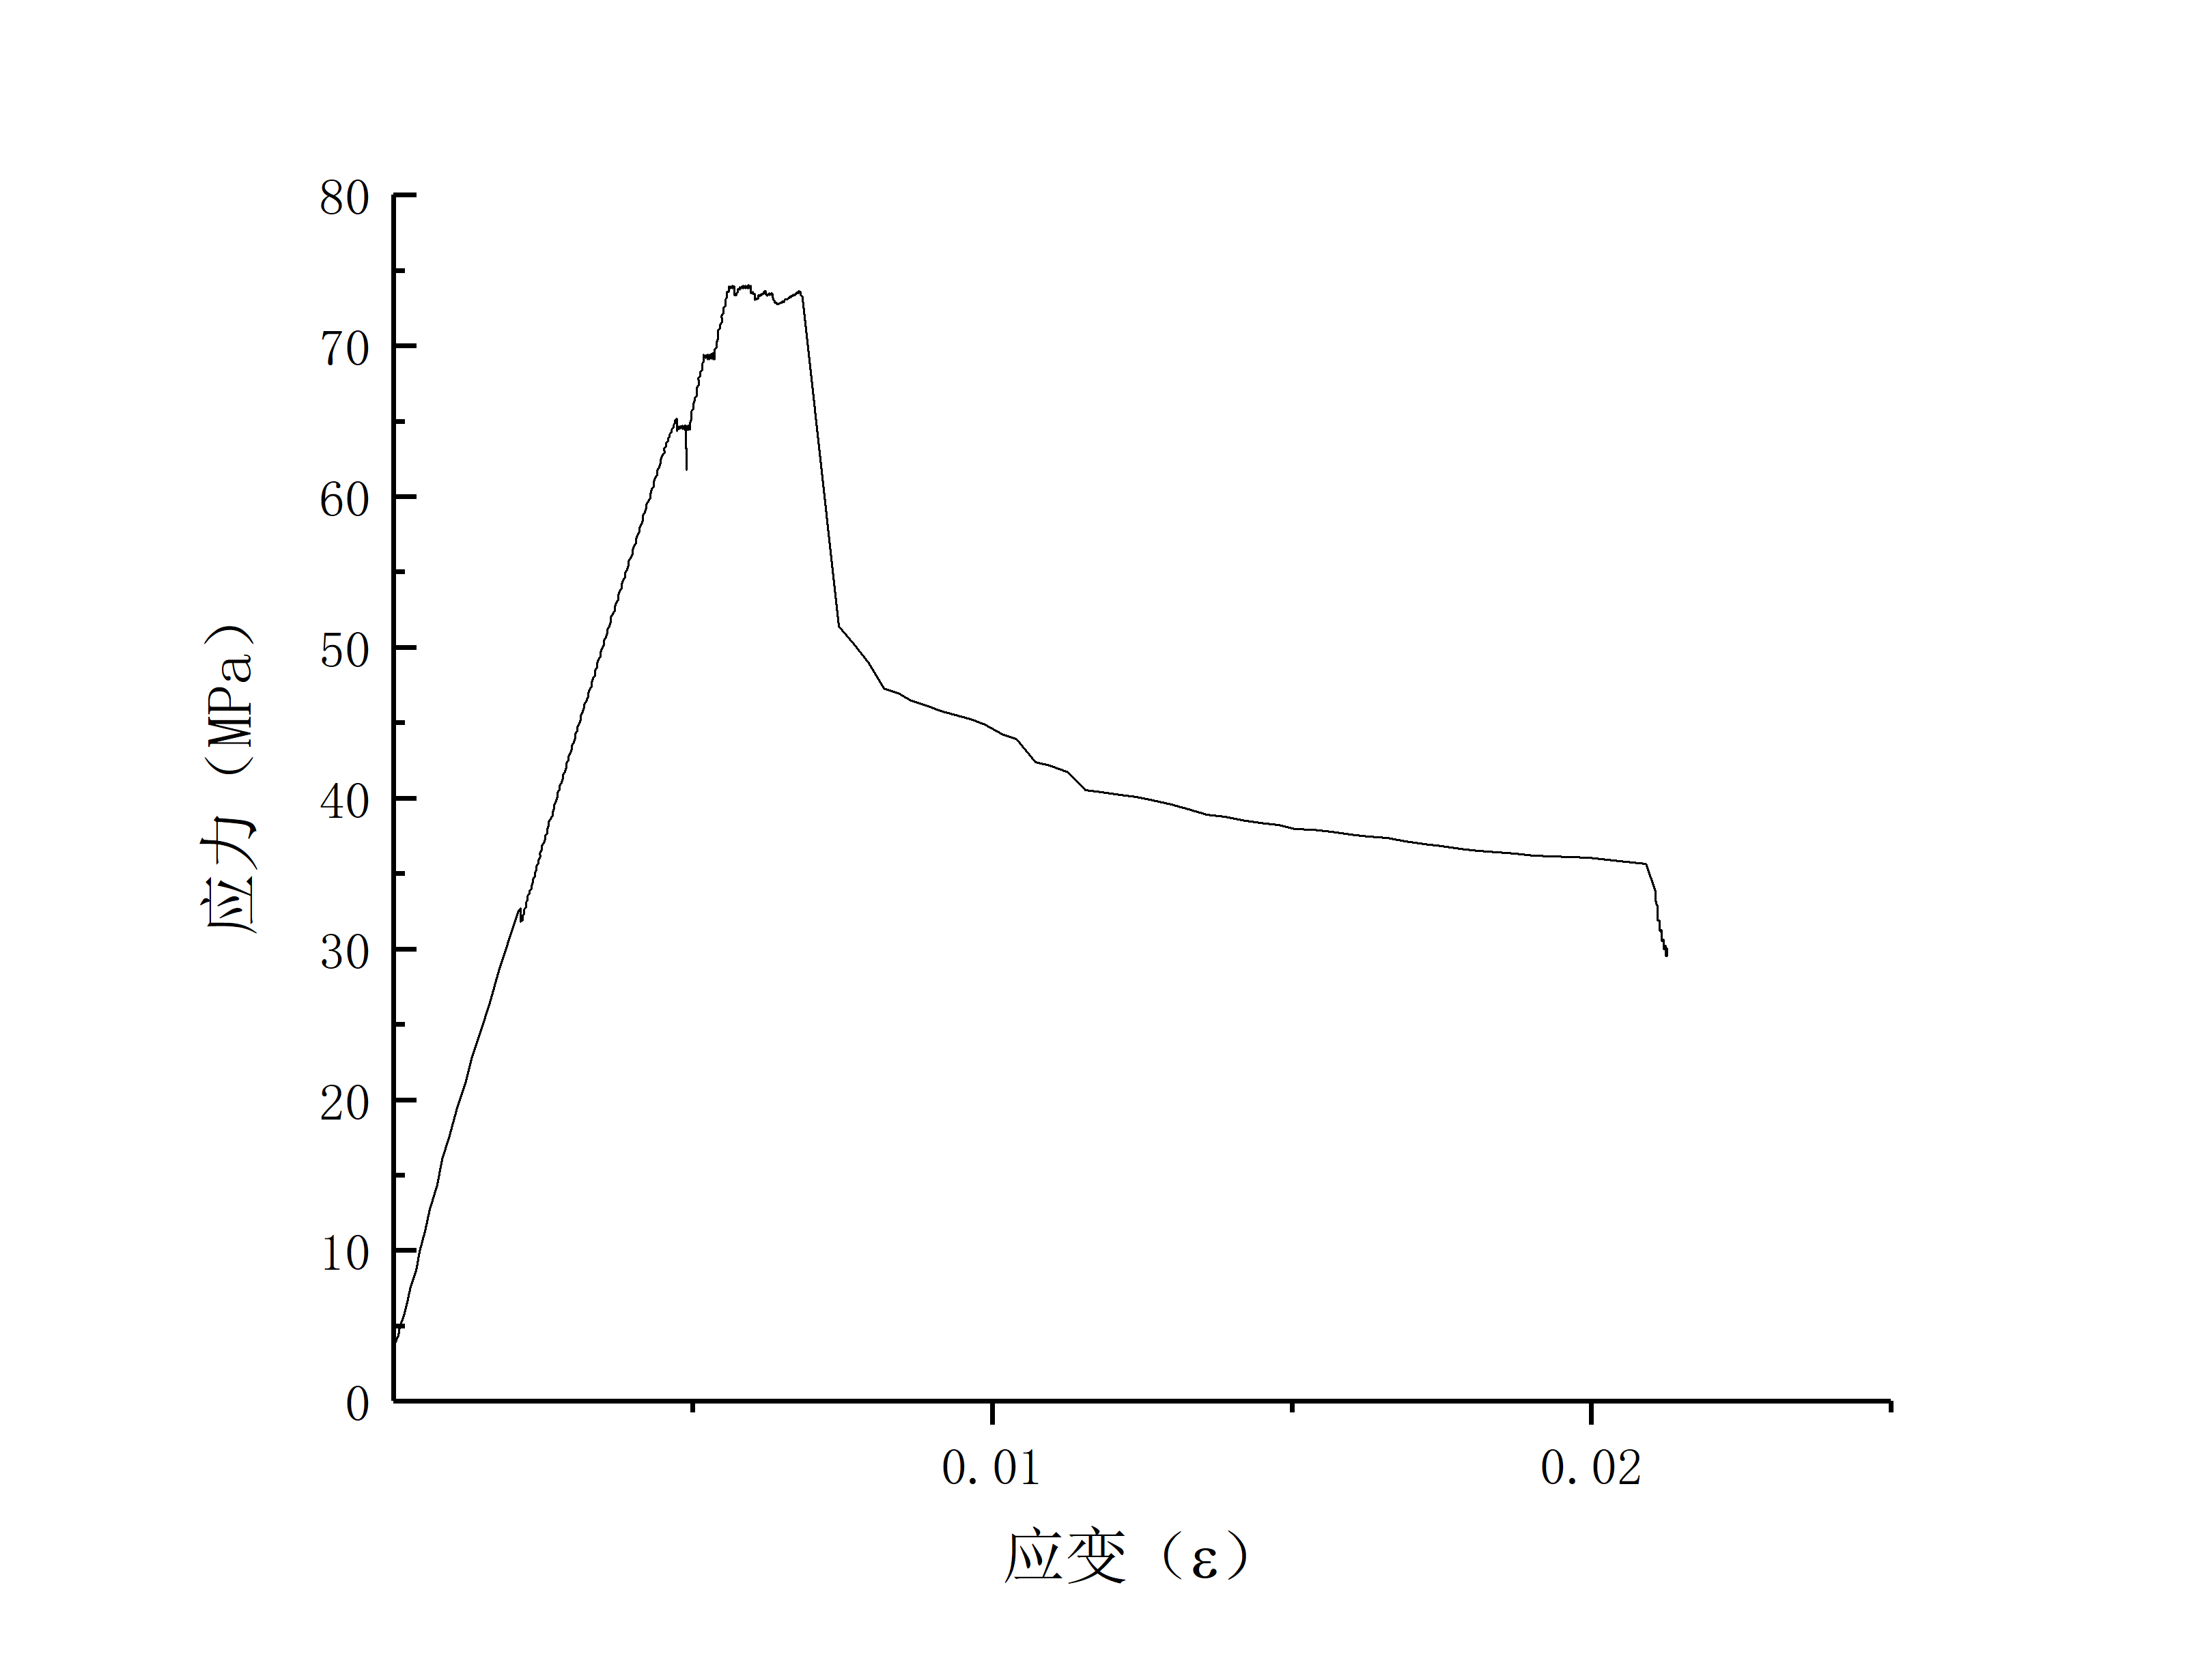
\includegraphics[width=1.1\textwidth]{img/chap2/stress-strain-D01.png}
        \end{minipage}
    }
    \subfigure[D-02]
    {
        \begin{minipage}{7cm}
            \centering
            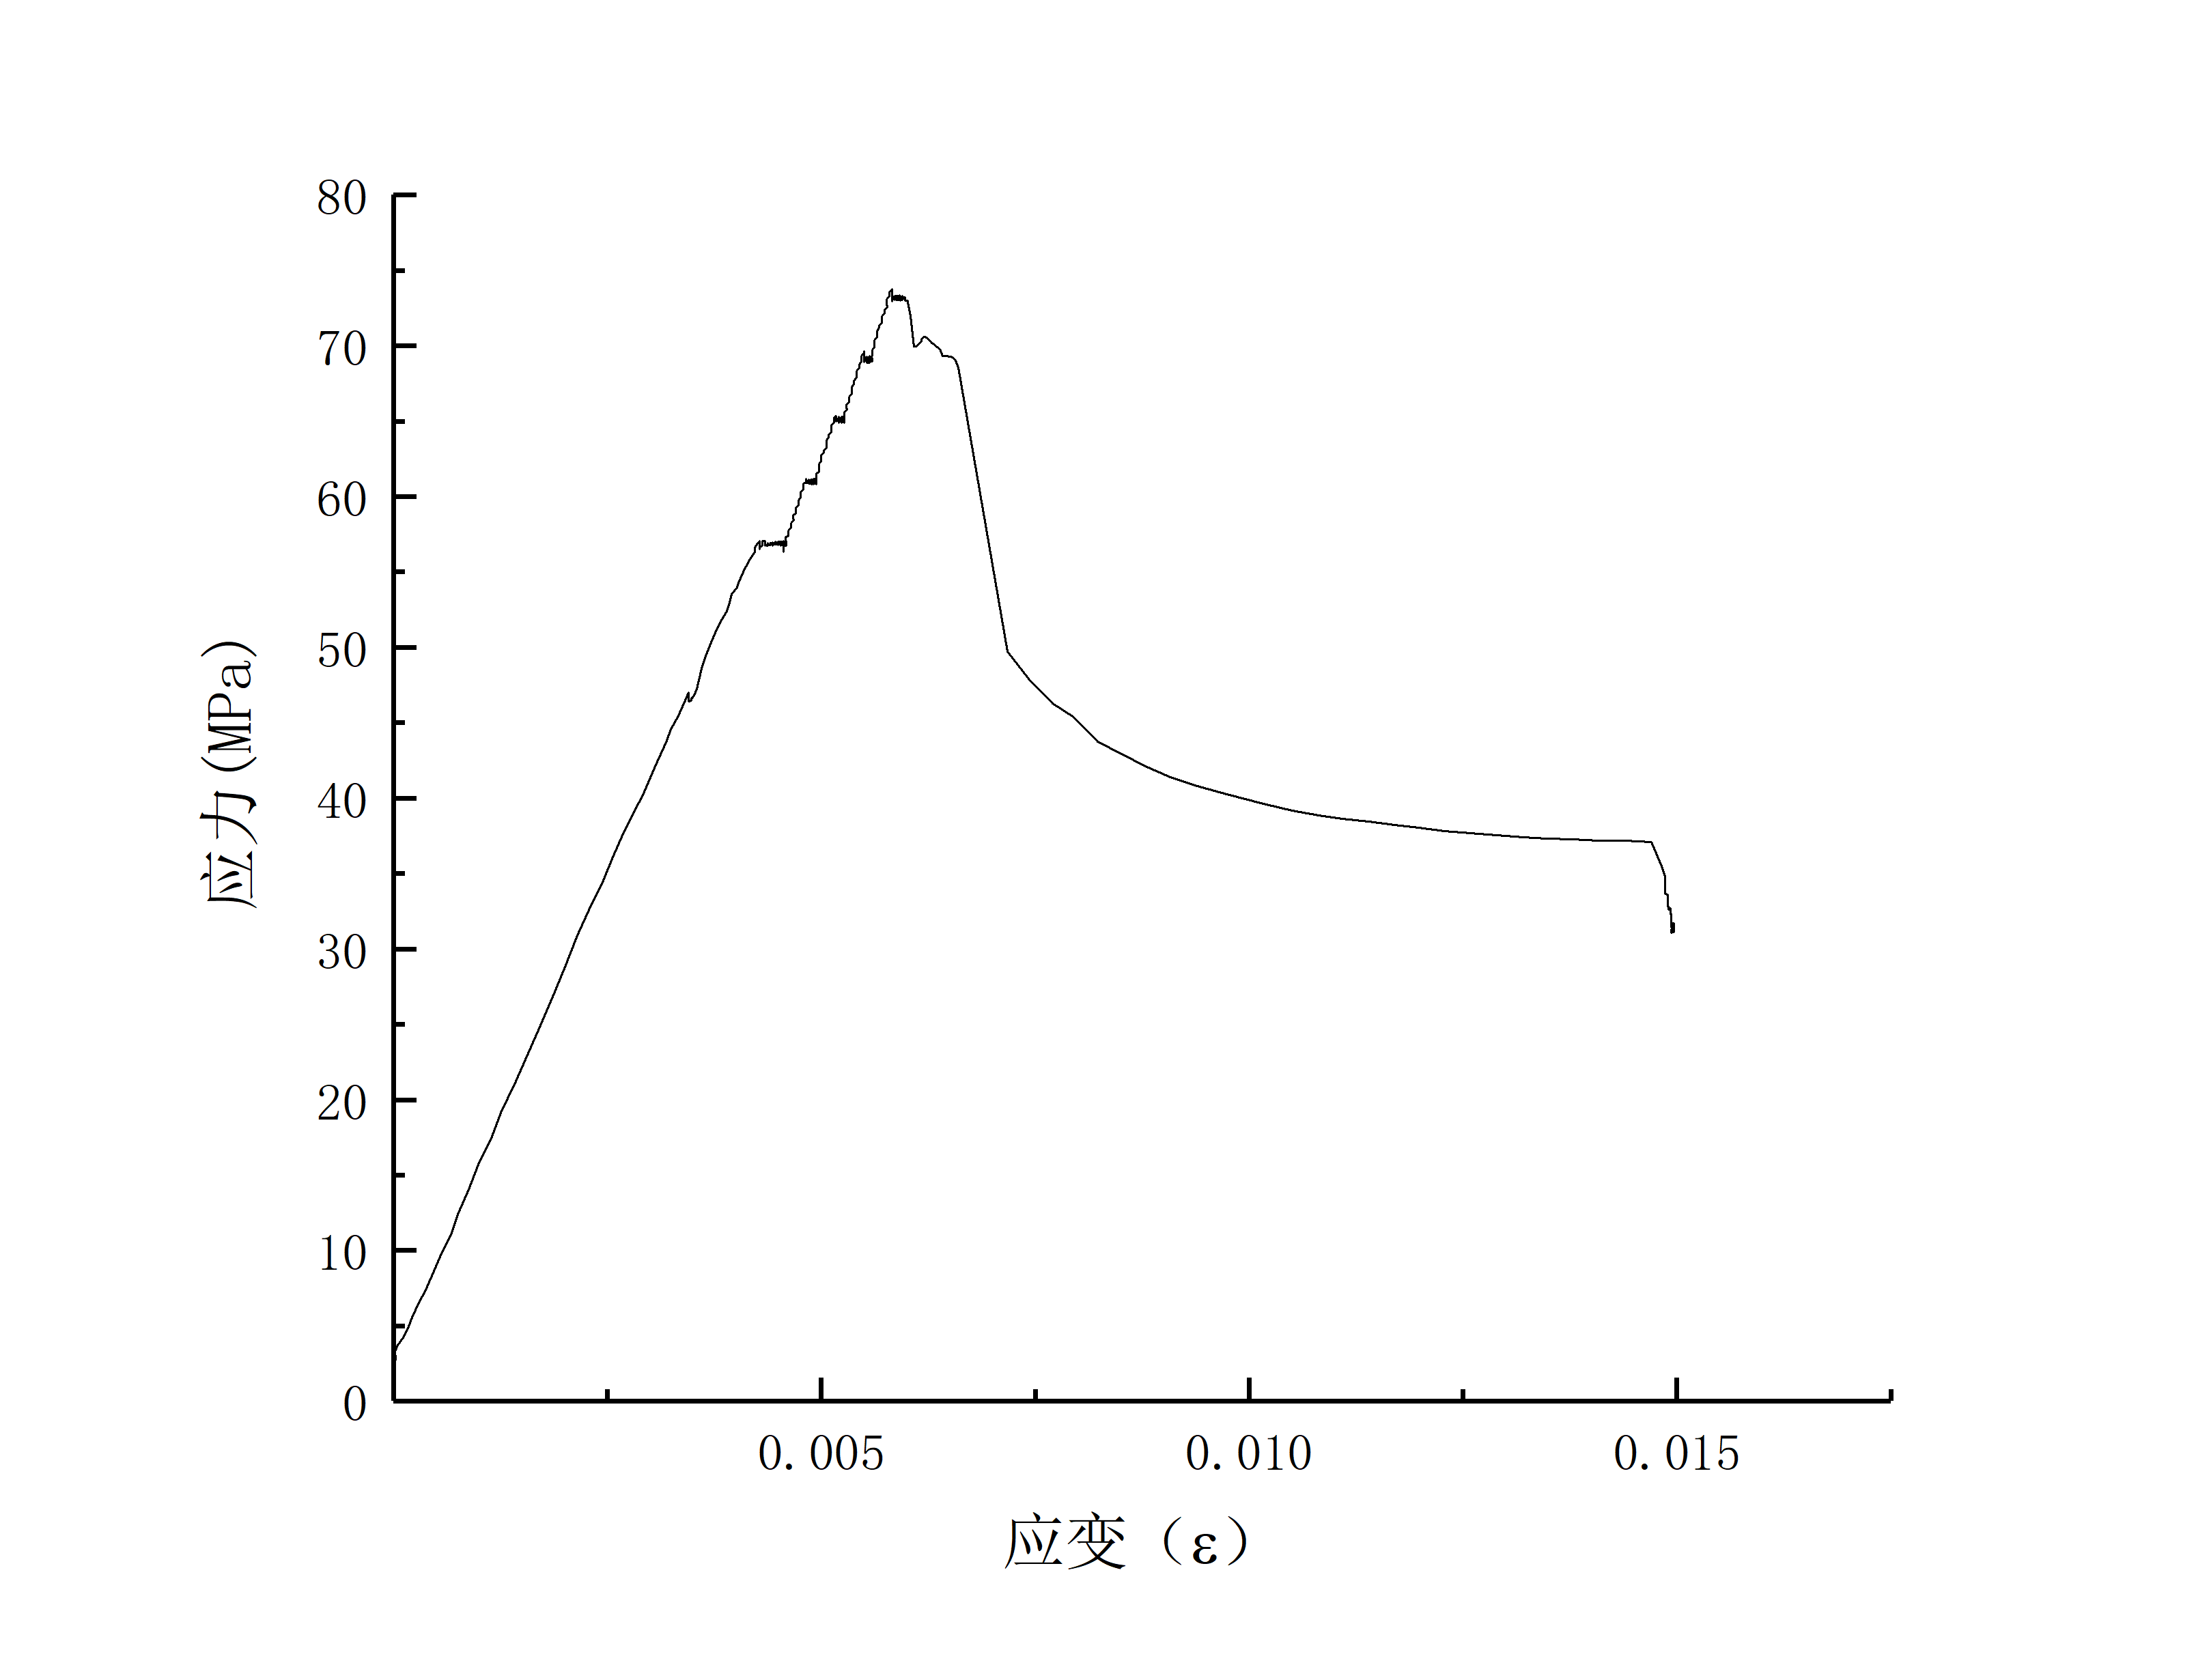
\includegraphics[width=1.1\textwidth]{img/chap2/stress-strain-D02.png}
        \end{minipage}
    }
	
    \subfigure[D-03]
    {
        \begin{minipage}{7cm}
            \centering
            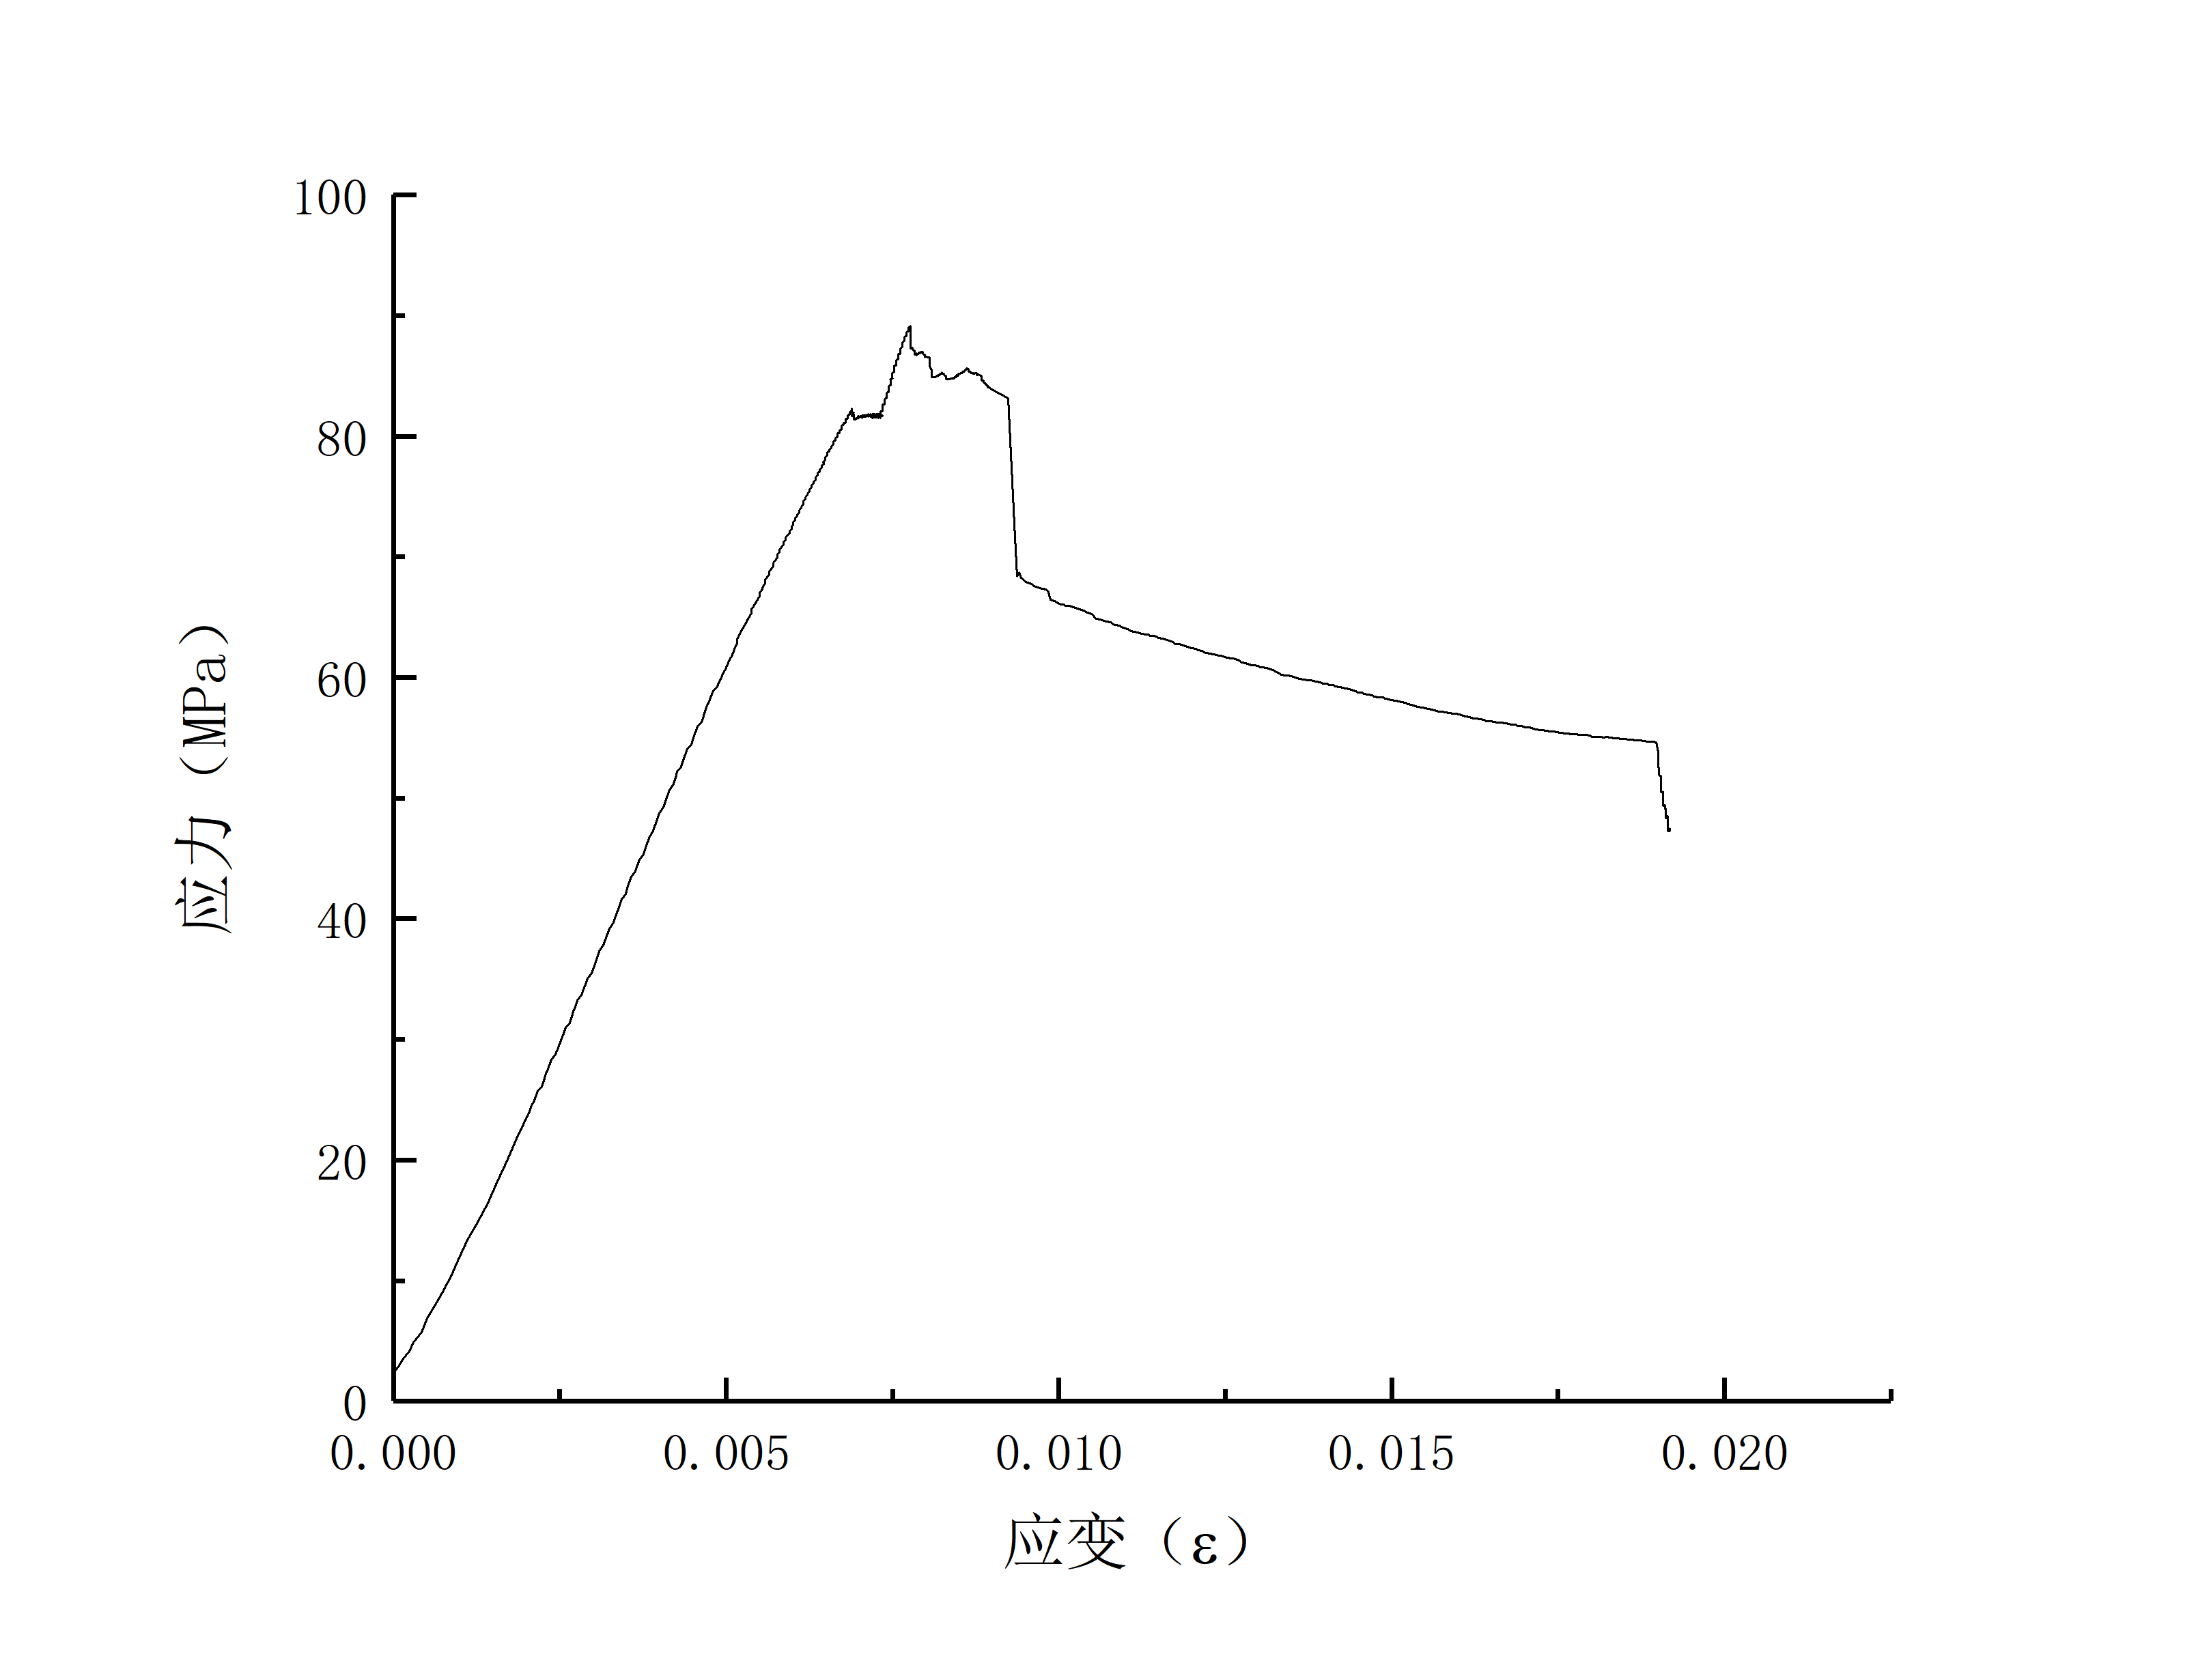
\includegraphics[width=1.1\textwidth]{img/chap2/stress-strain-D03.png}
        \end{minipage}
    }
    \centering
    \caption{三轴流变应力-应变曲线图}
    \label{fig:2-15}
\end{figure}



\begin{figure}[ht!]
    \centering
    \subfigure[C-01]
    {
        \begin{minipage}{7cm}
            \centering
            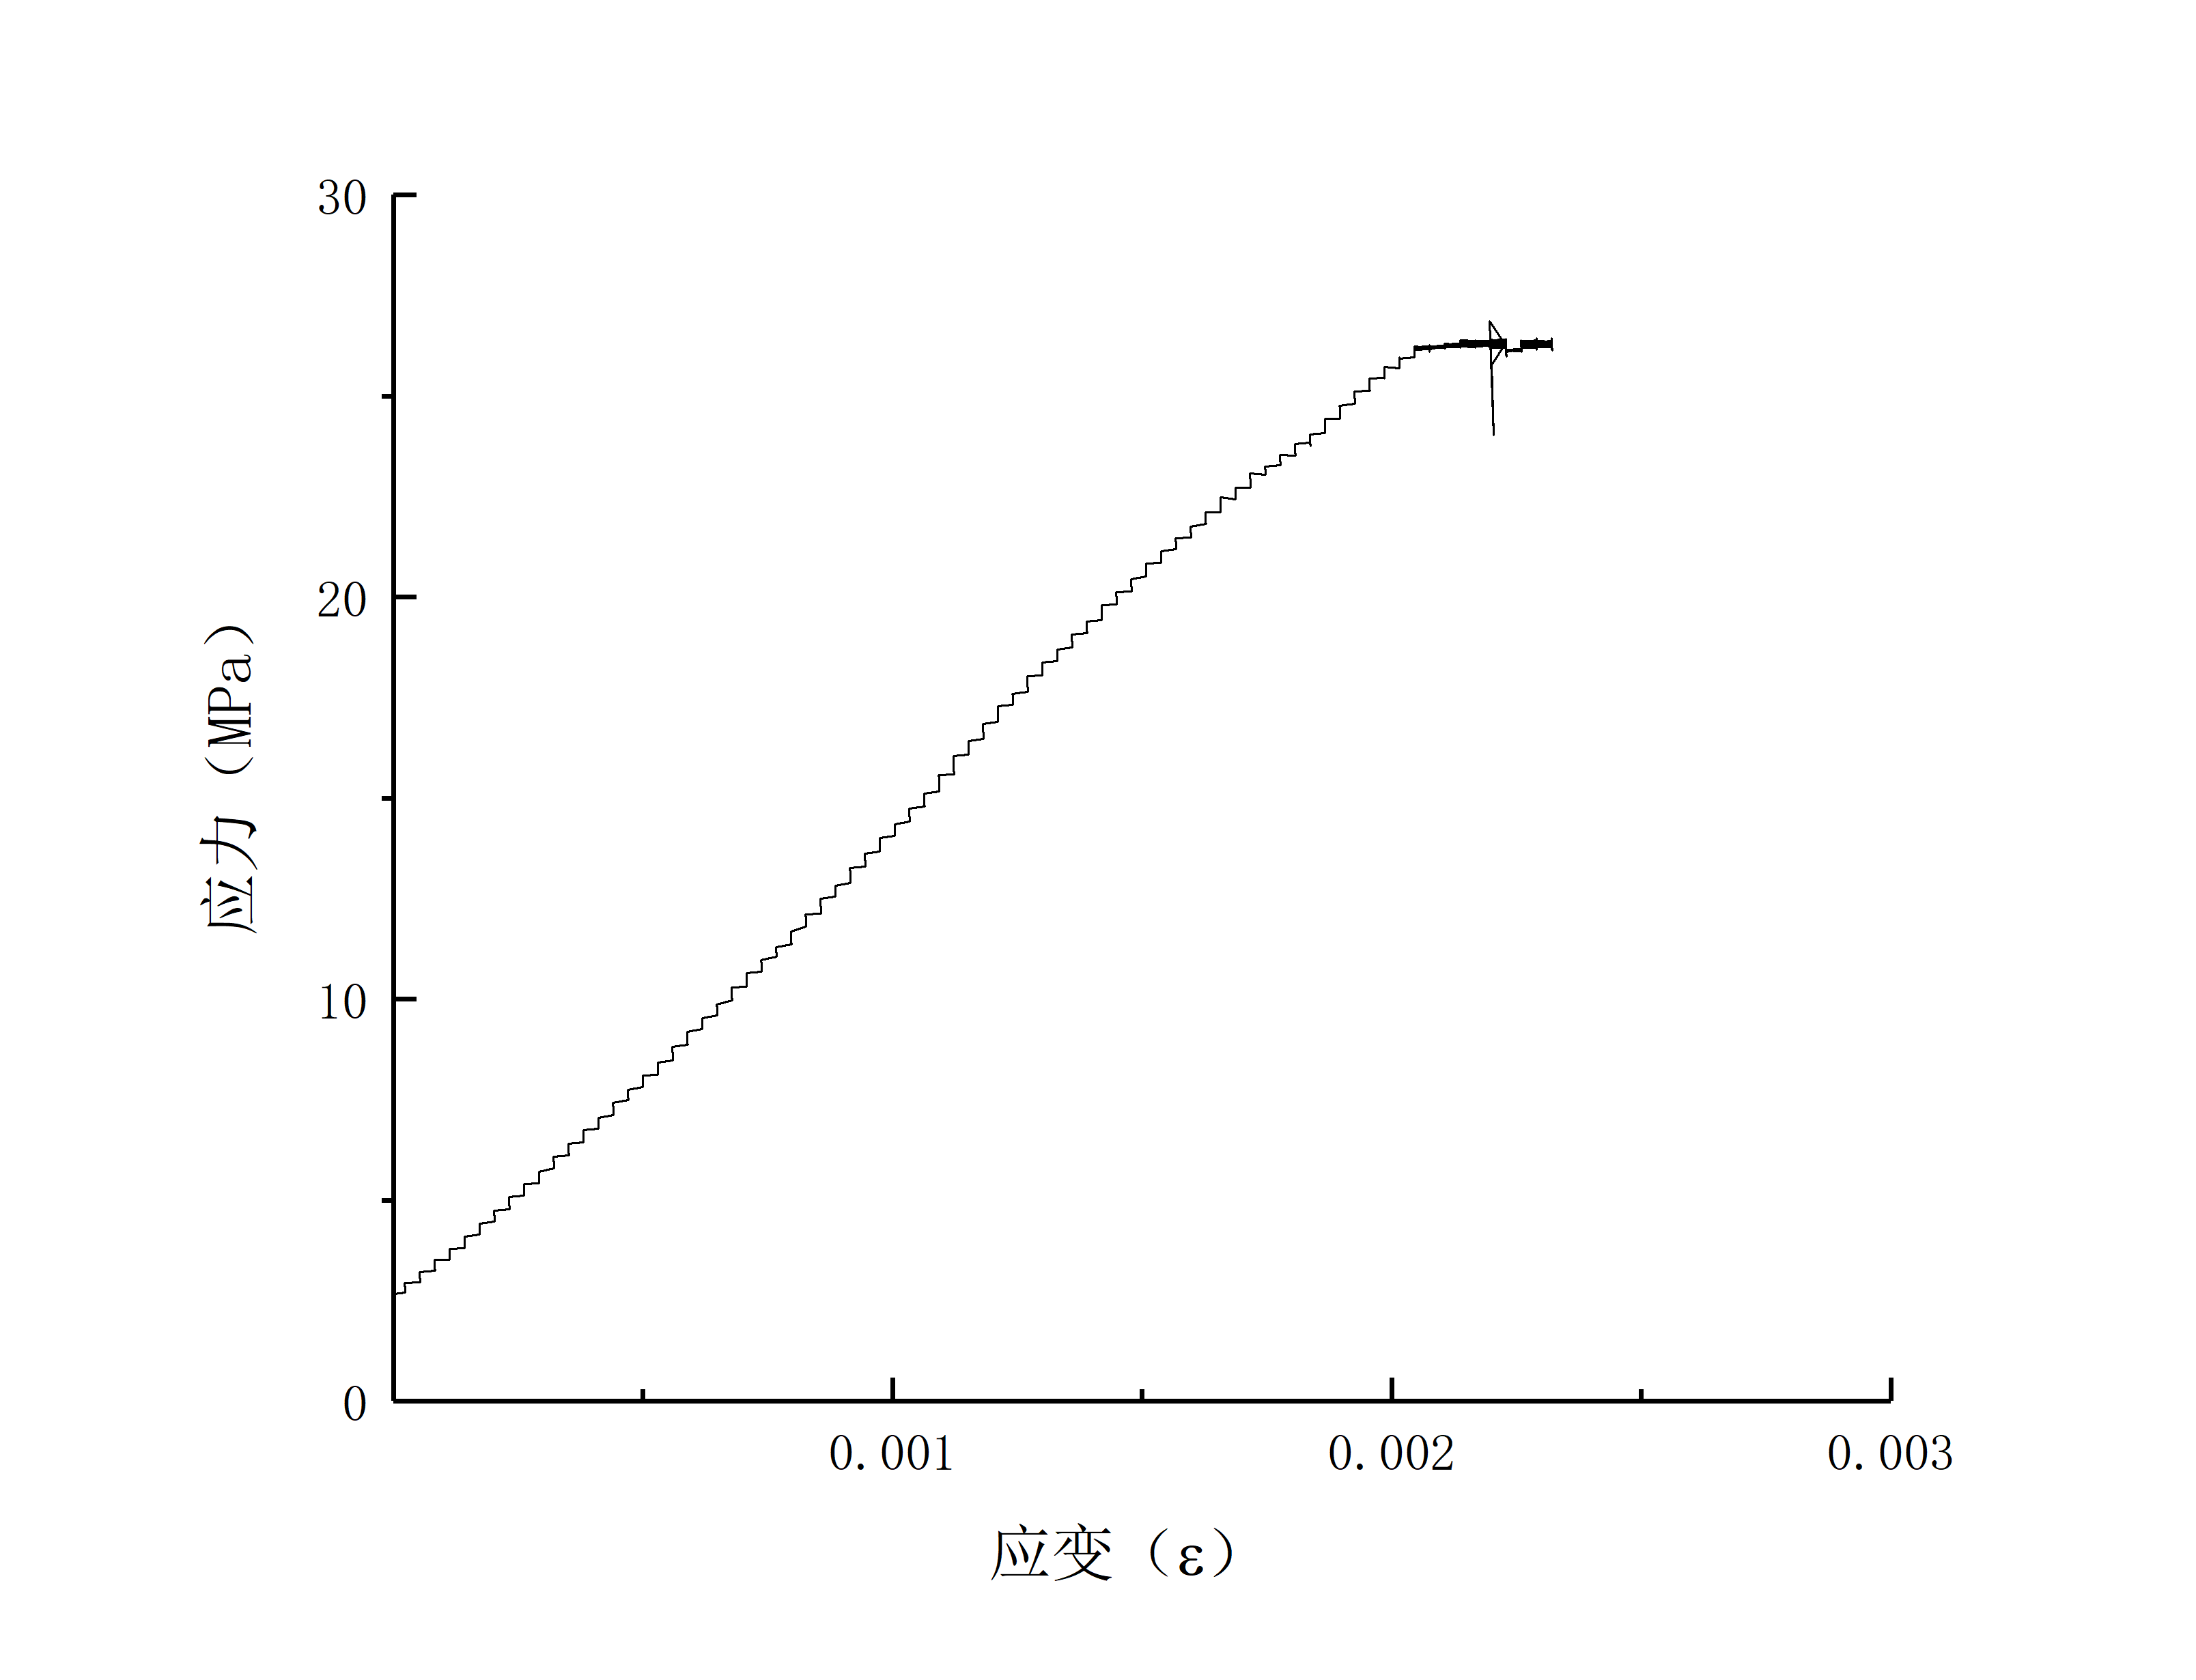
\includegraphics[width=1.1\textwidth]{img/chap2/stress-strain-C01.png}
        \end{minipage}
    }
    \subfigure[C-02]
    {
        \begin{minipage}{7cm}
            \centering
            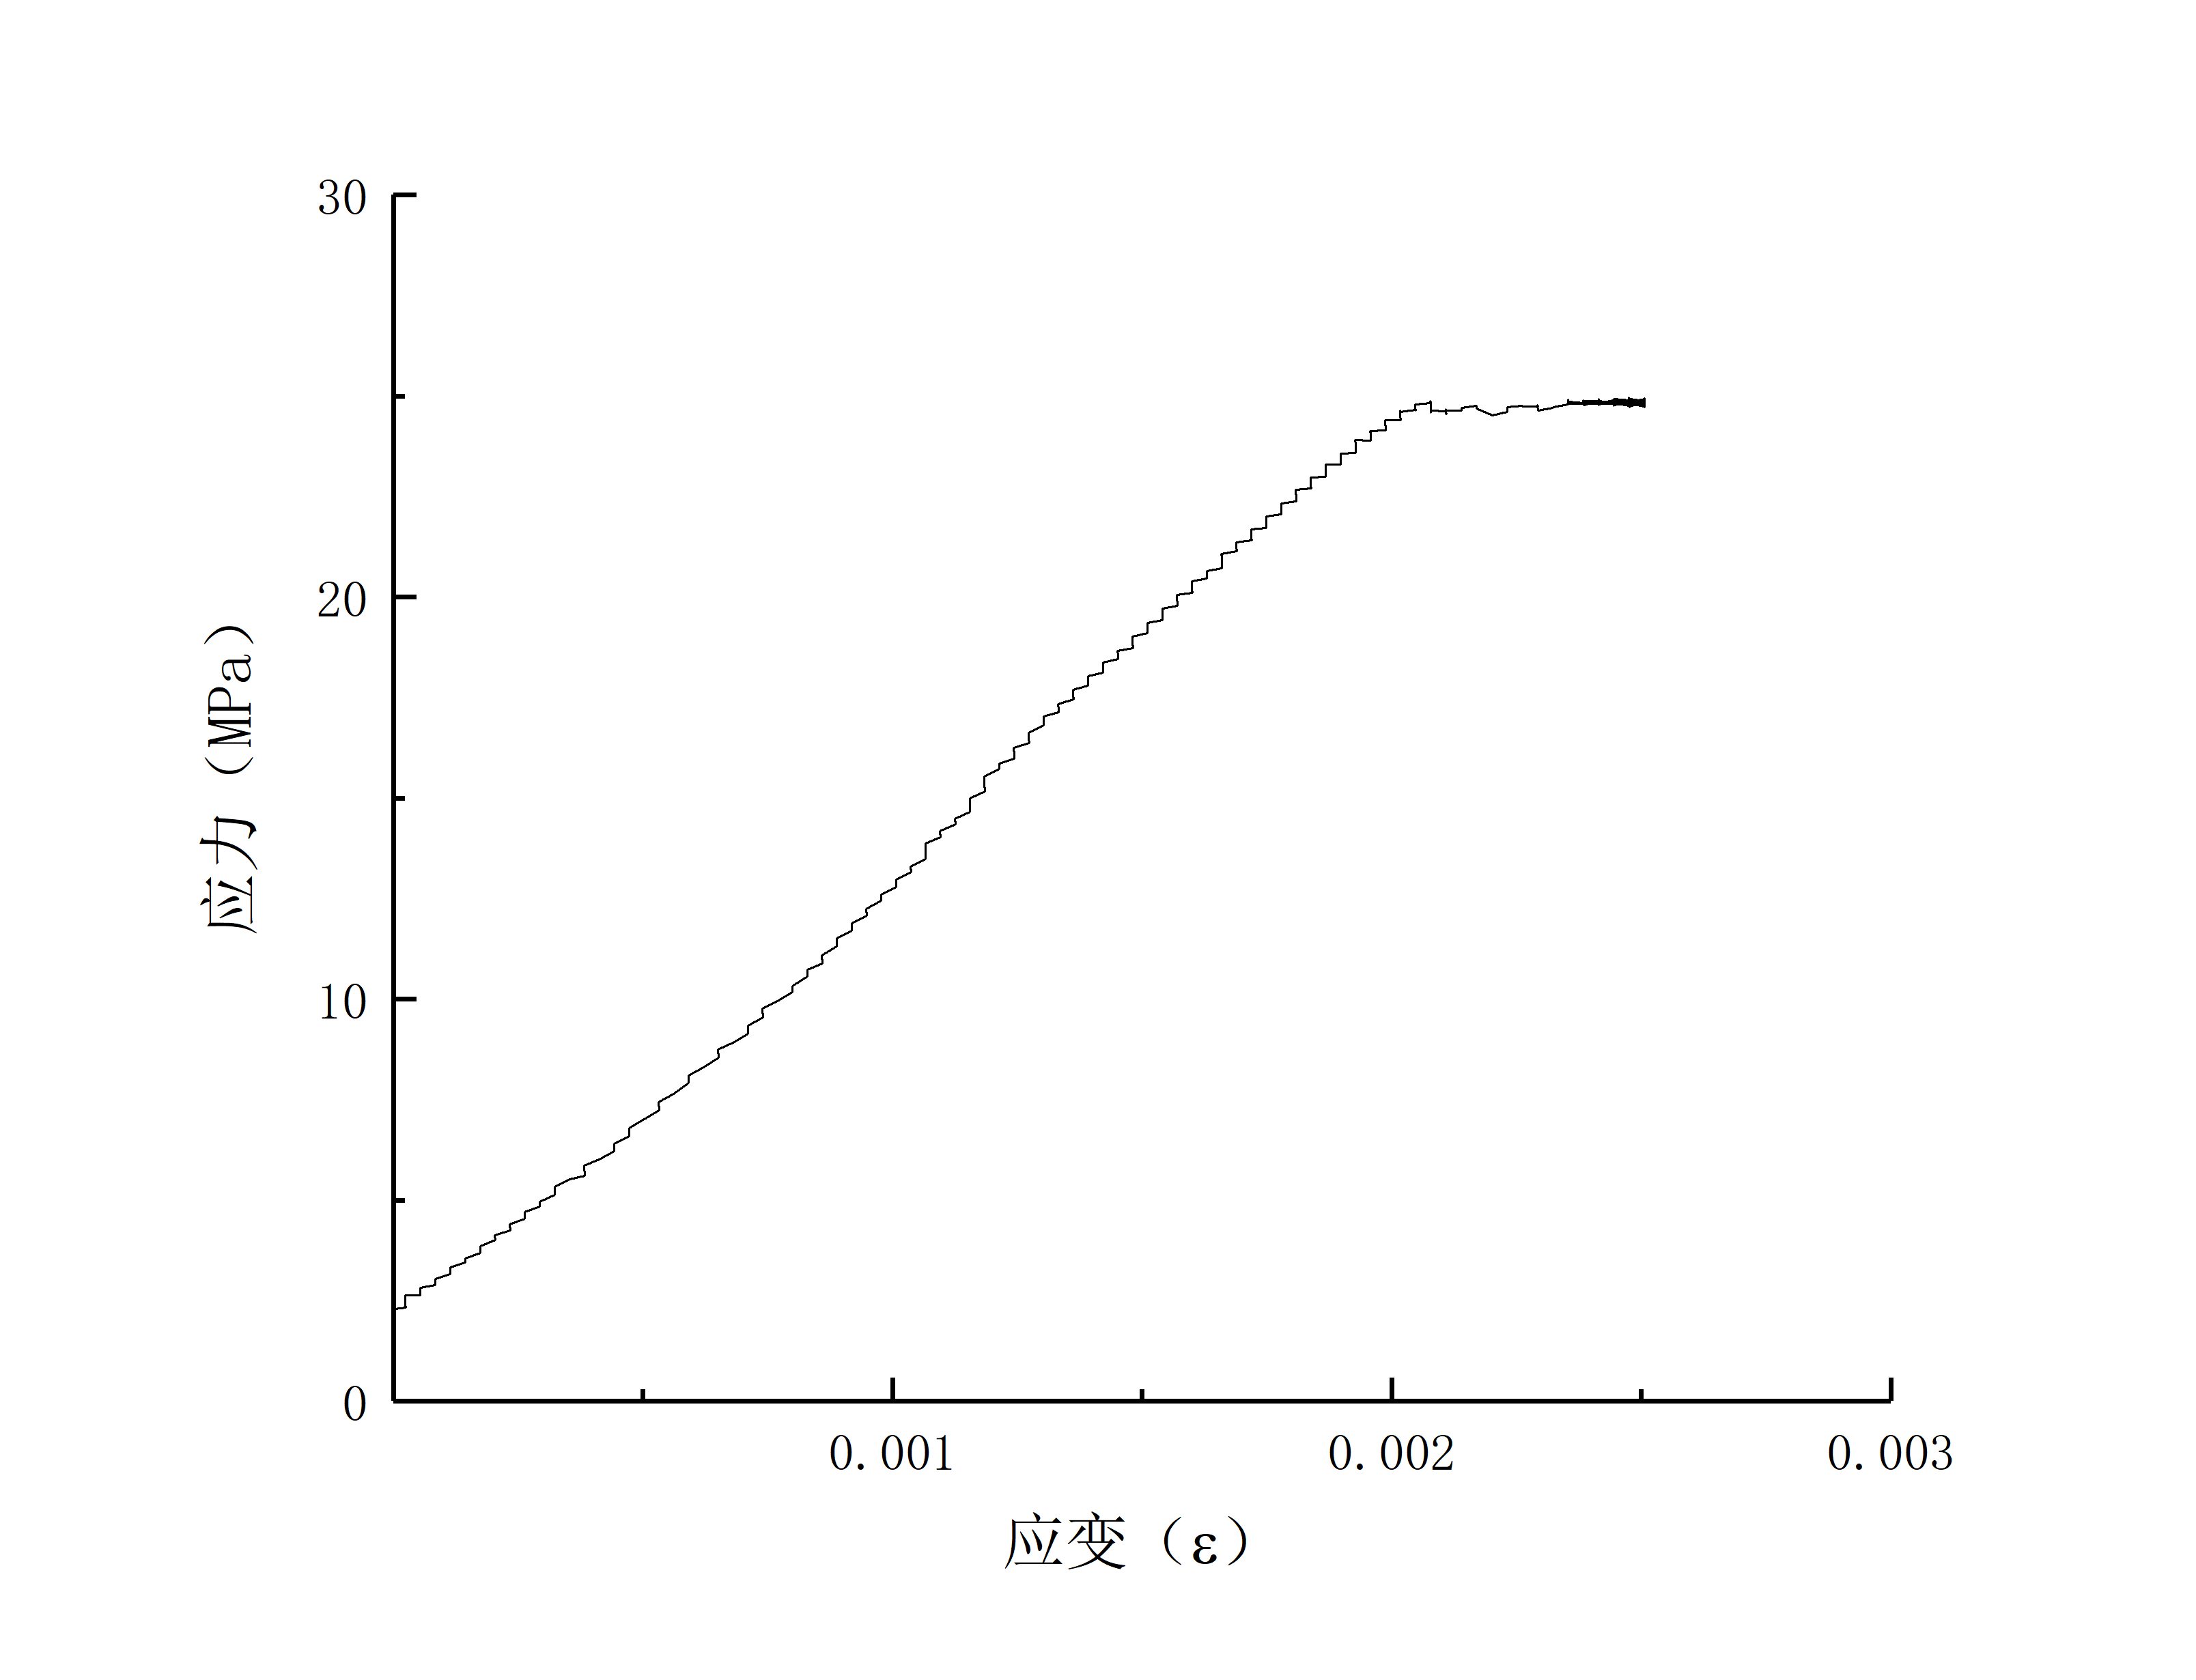
\includegraphics[width=1.1\textwidth]{img/chap2/stress-strain-C02.png}
        \end{minipage}
    }
	
    \subfigure[C-03]
    {
        \begin{minipage}{7cm}
            \centering
            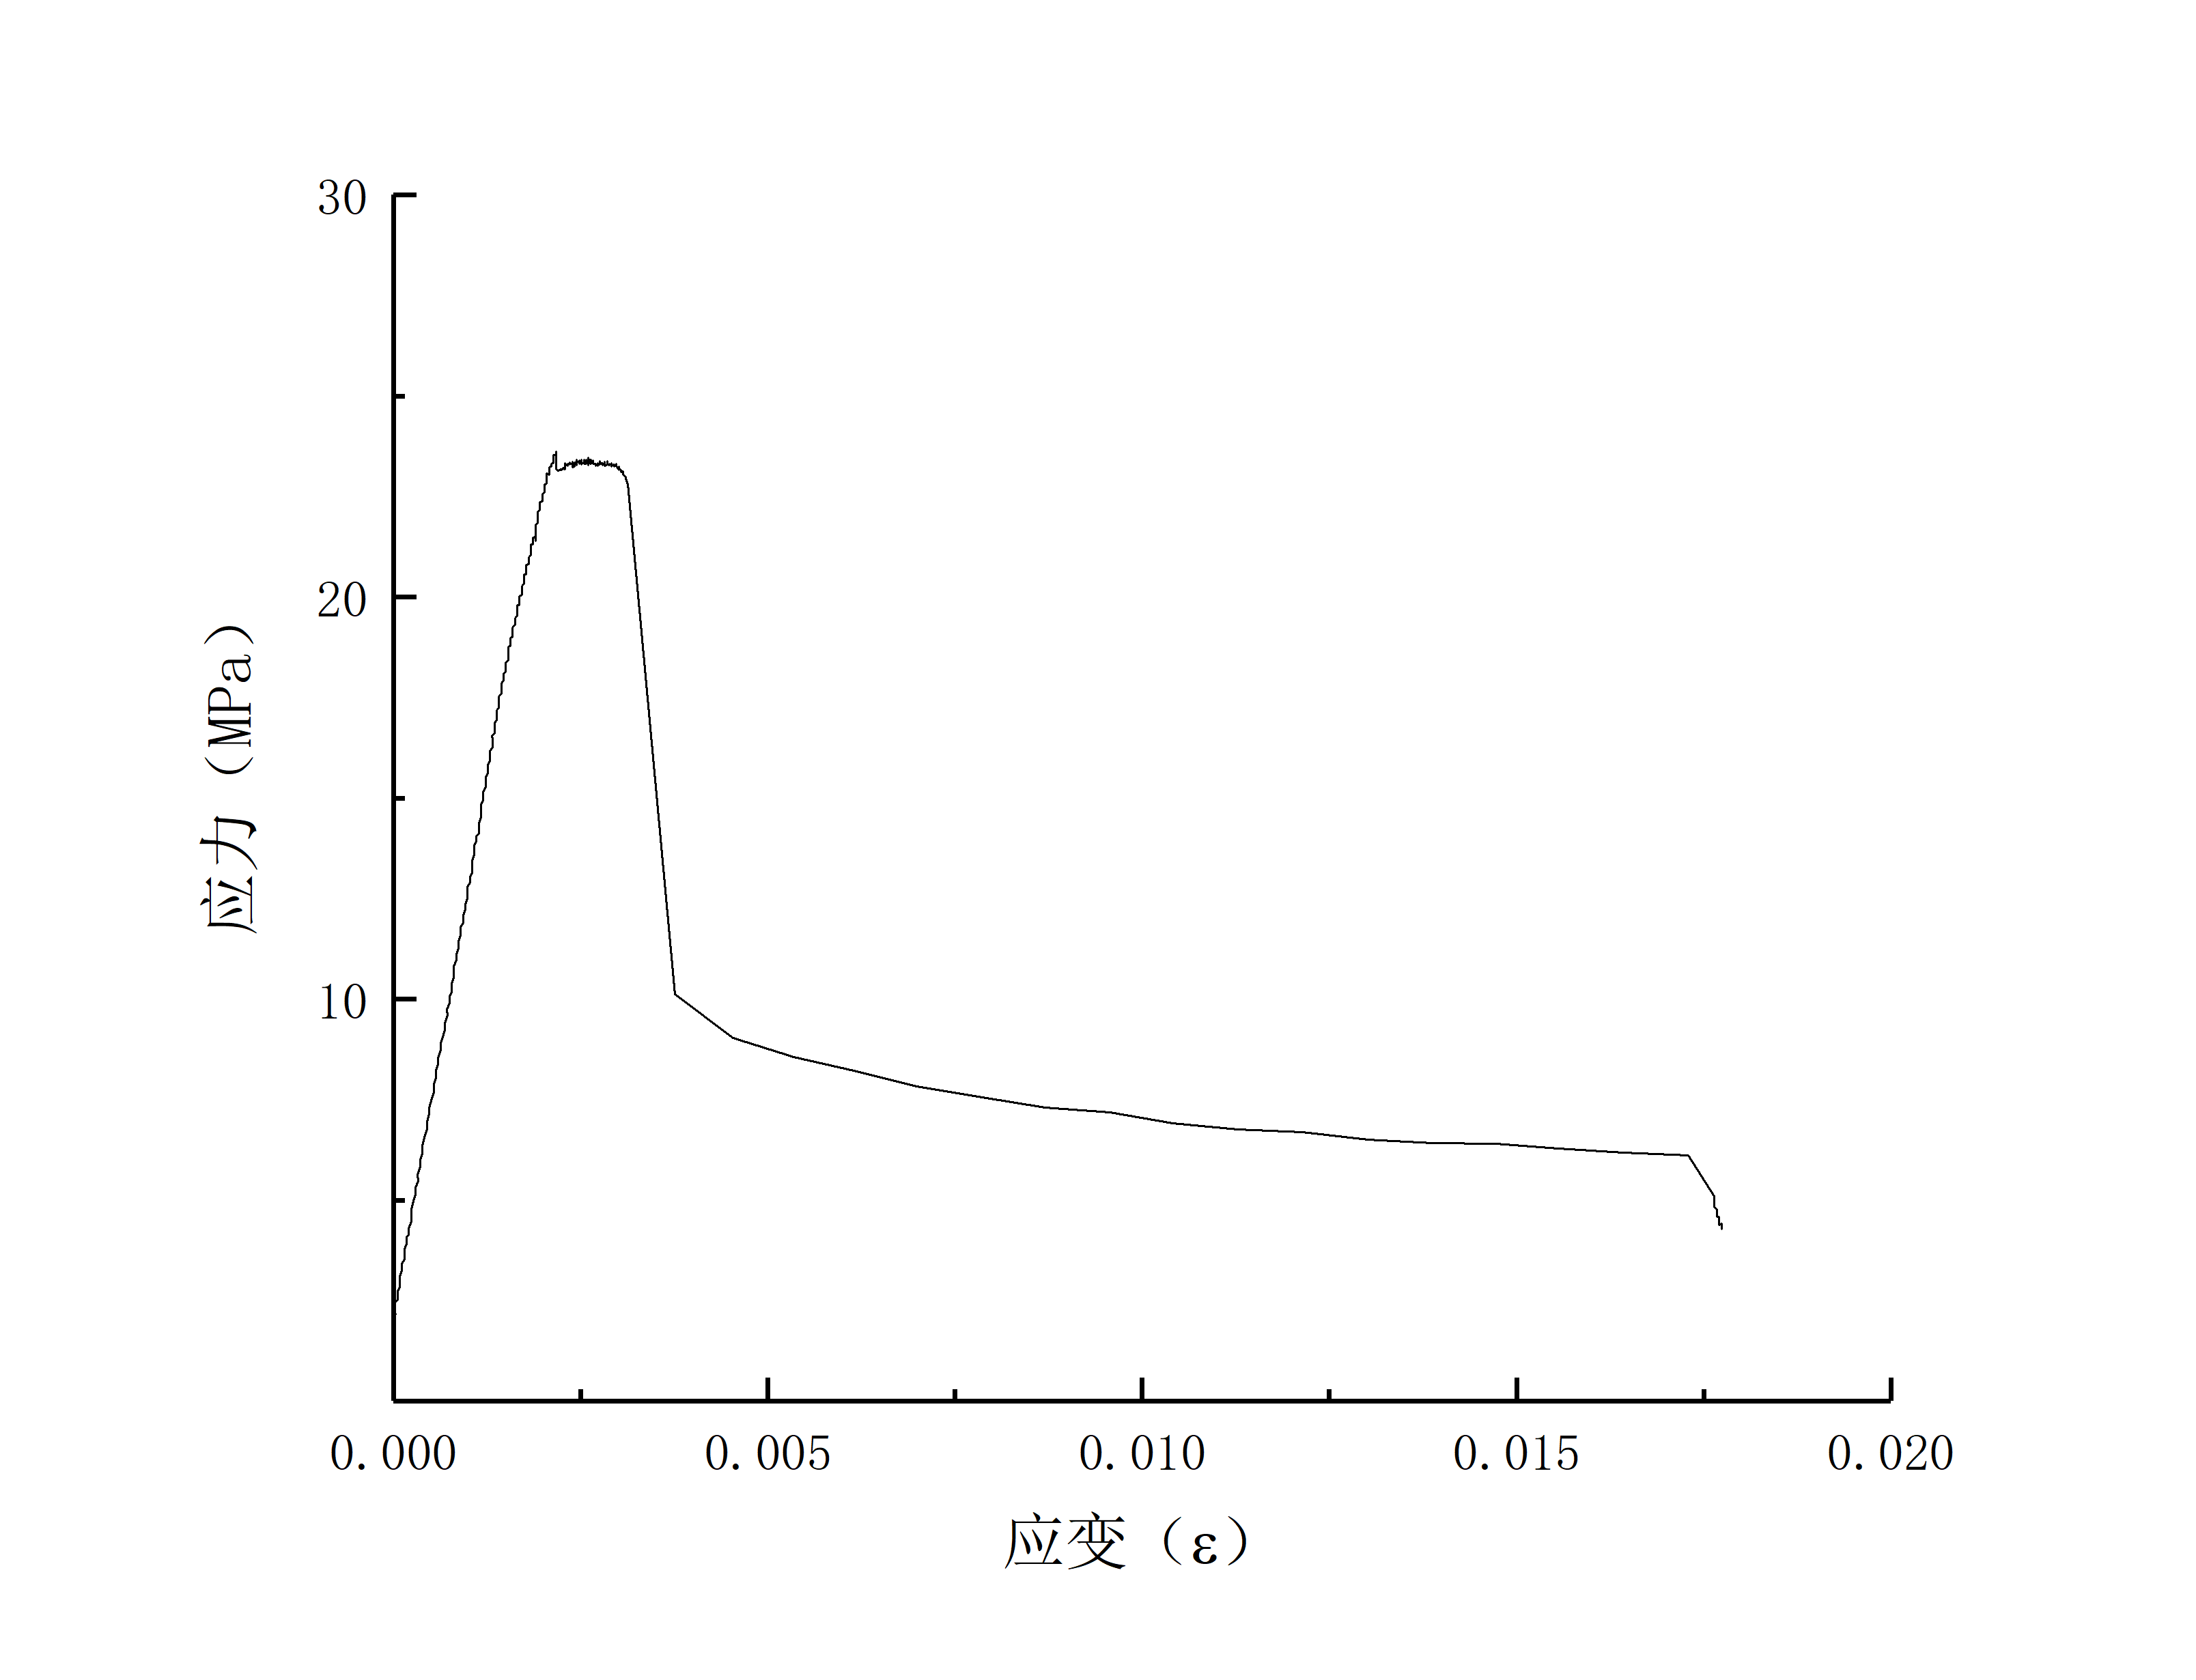
\includegraphics[width=1.1\textwidth]{img/chap2/stress-strain-C03.png}
        \end{minipage}
    }
    \subfigure[C-04]
    {
        \begin{minipage}{7cm}
            \centering
            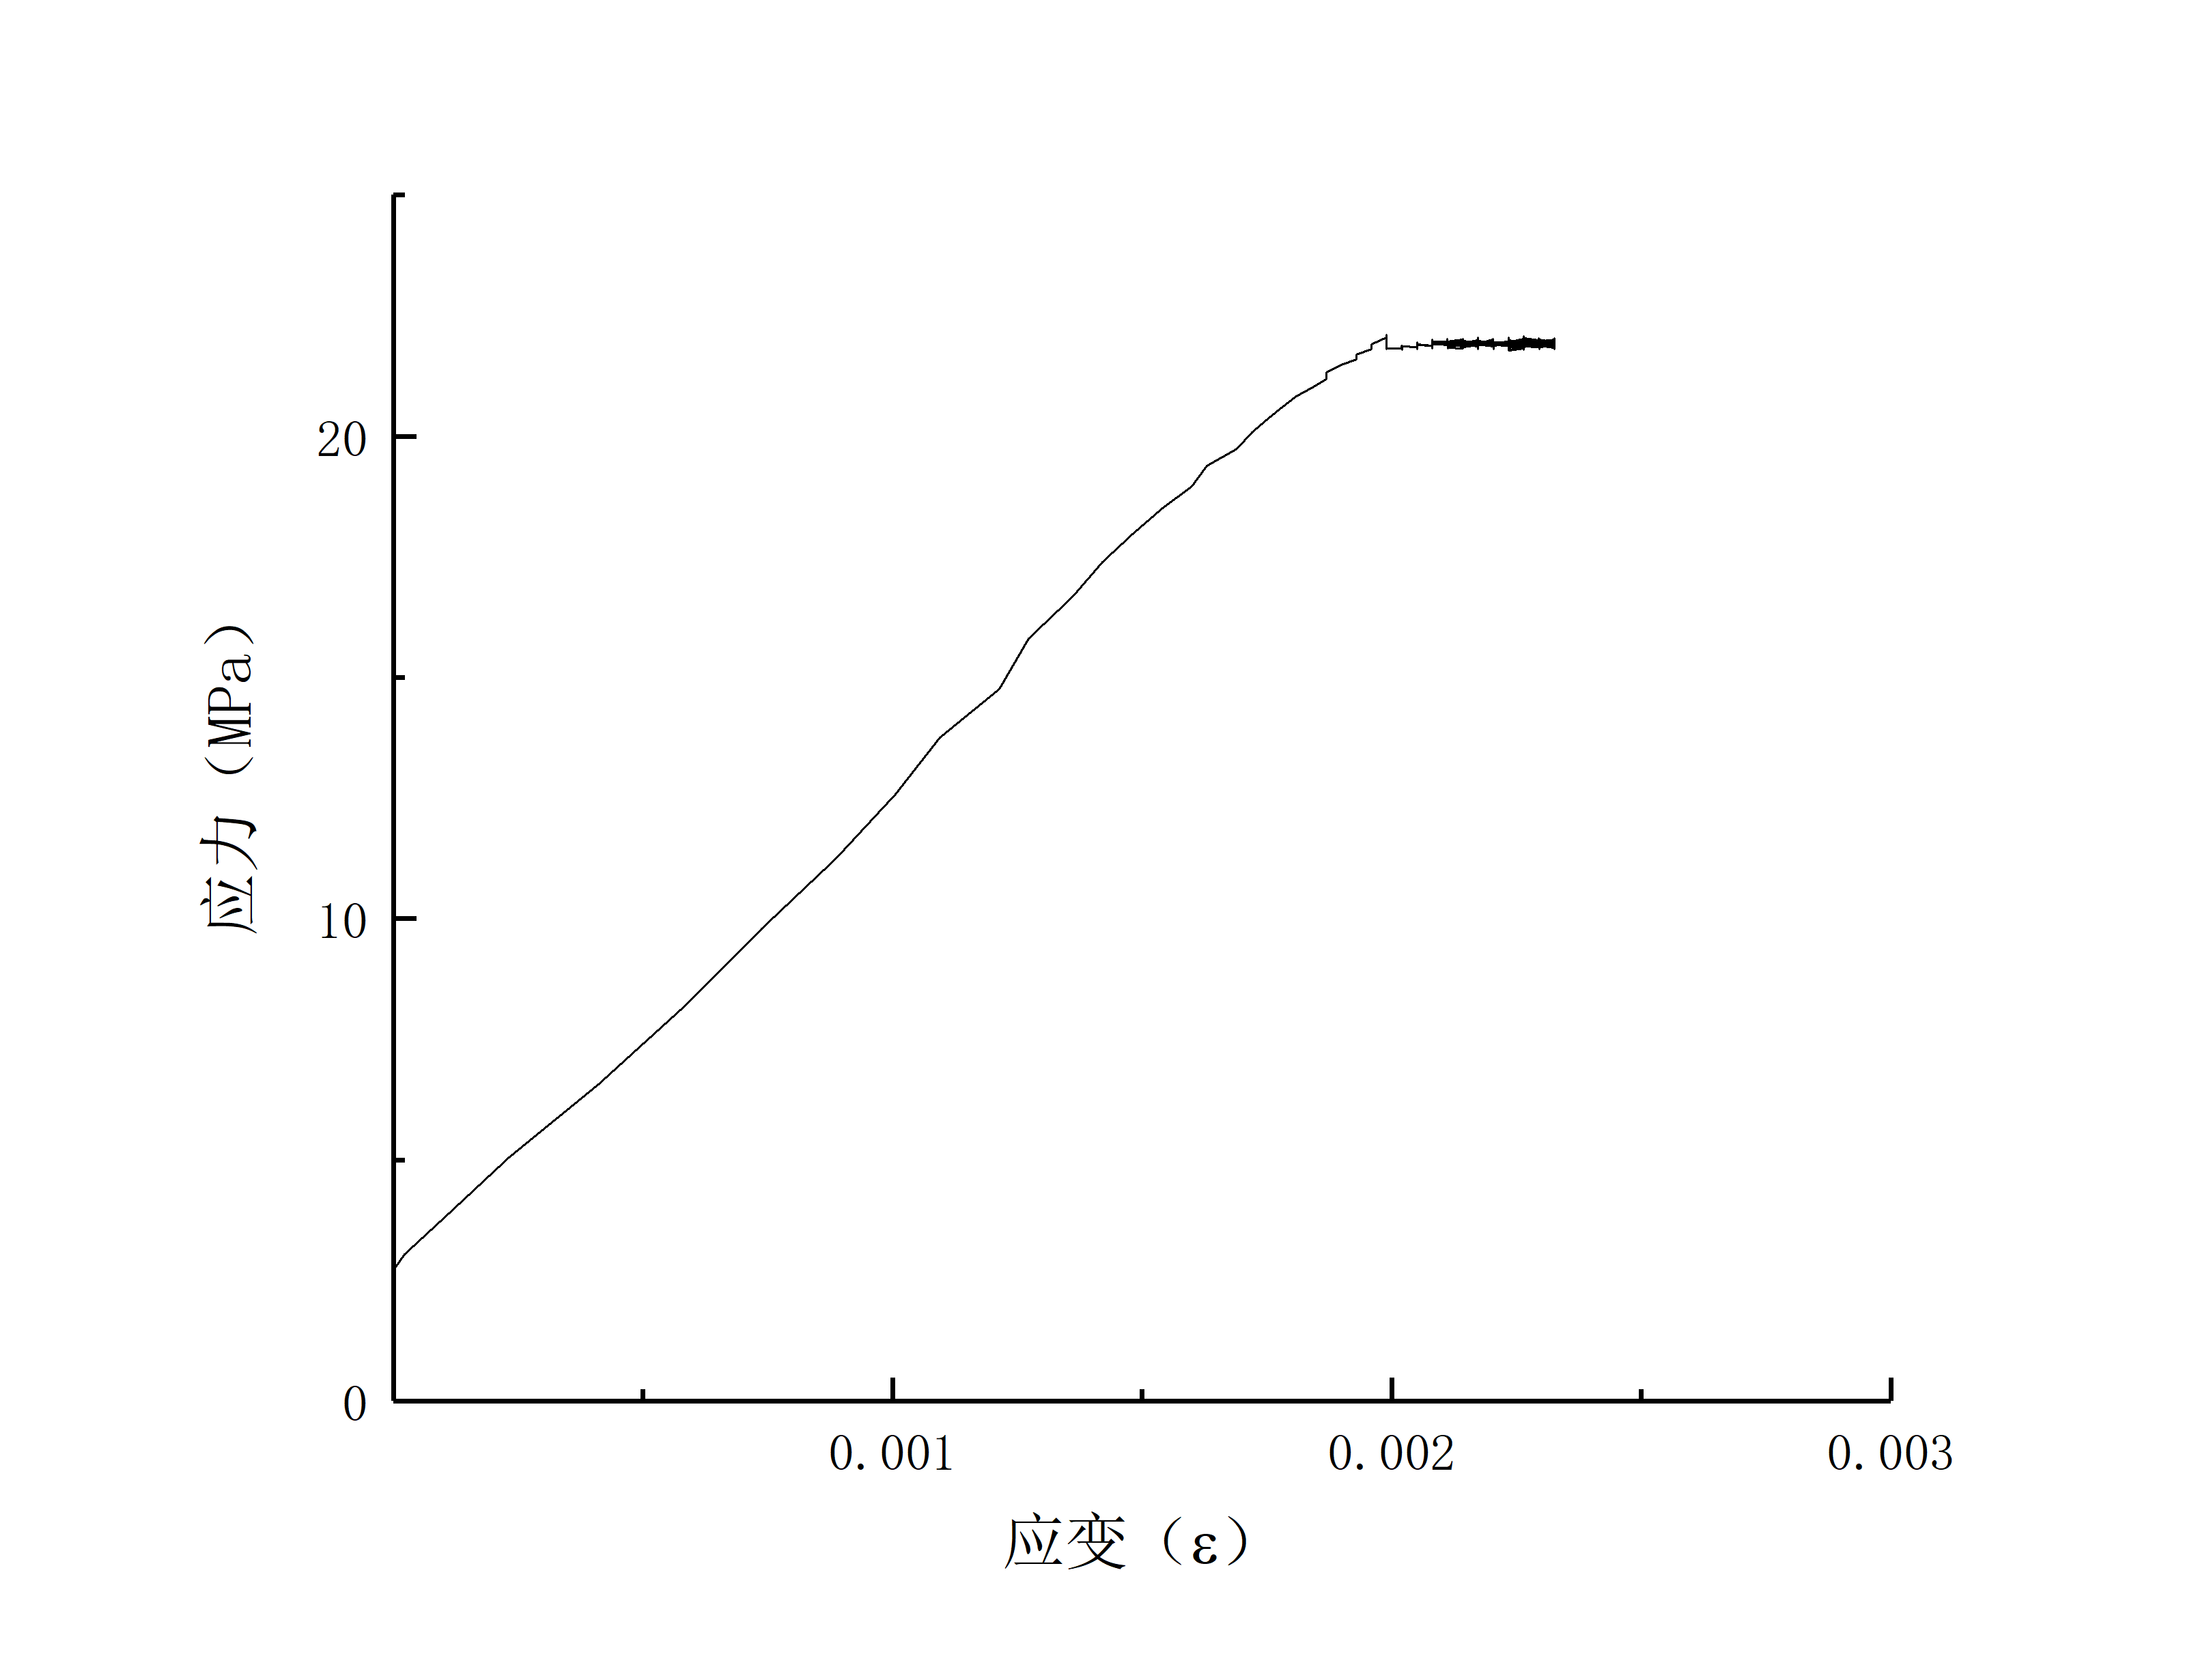
\includegraphics[width=1.1\textwidth]{img/chap2/stress-strain-C04.png}
        \end{minipage}
    }
    \centering
    \subfigure[C-05]
    {
        \begin{minipage}{7cm}
            \centering
            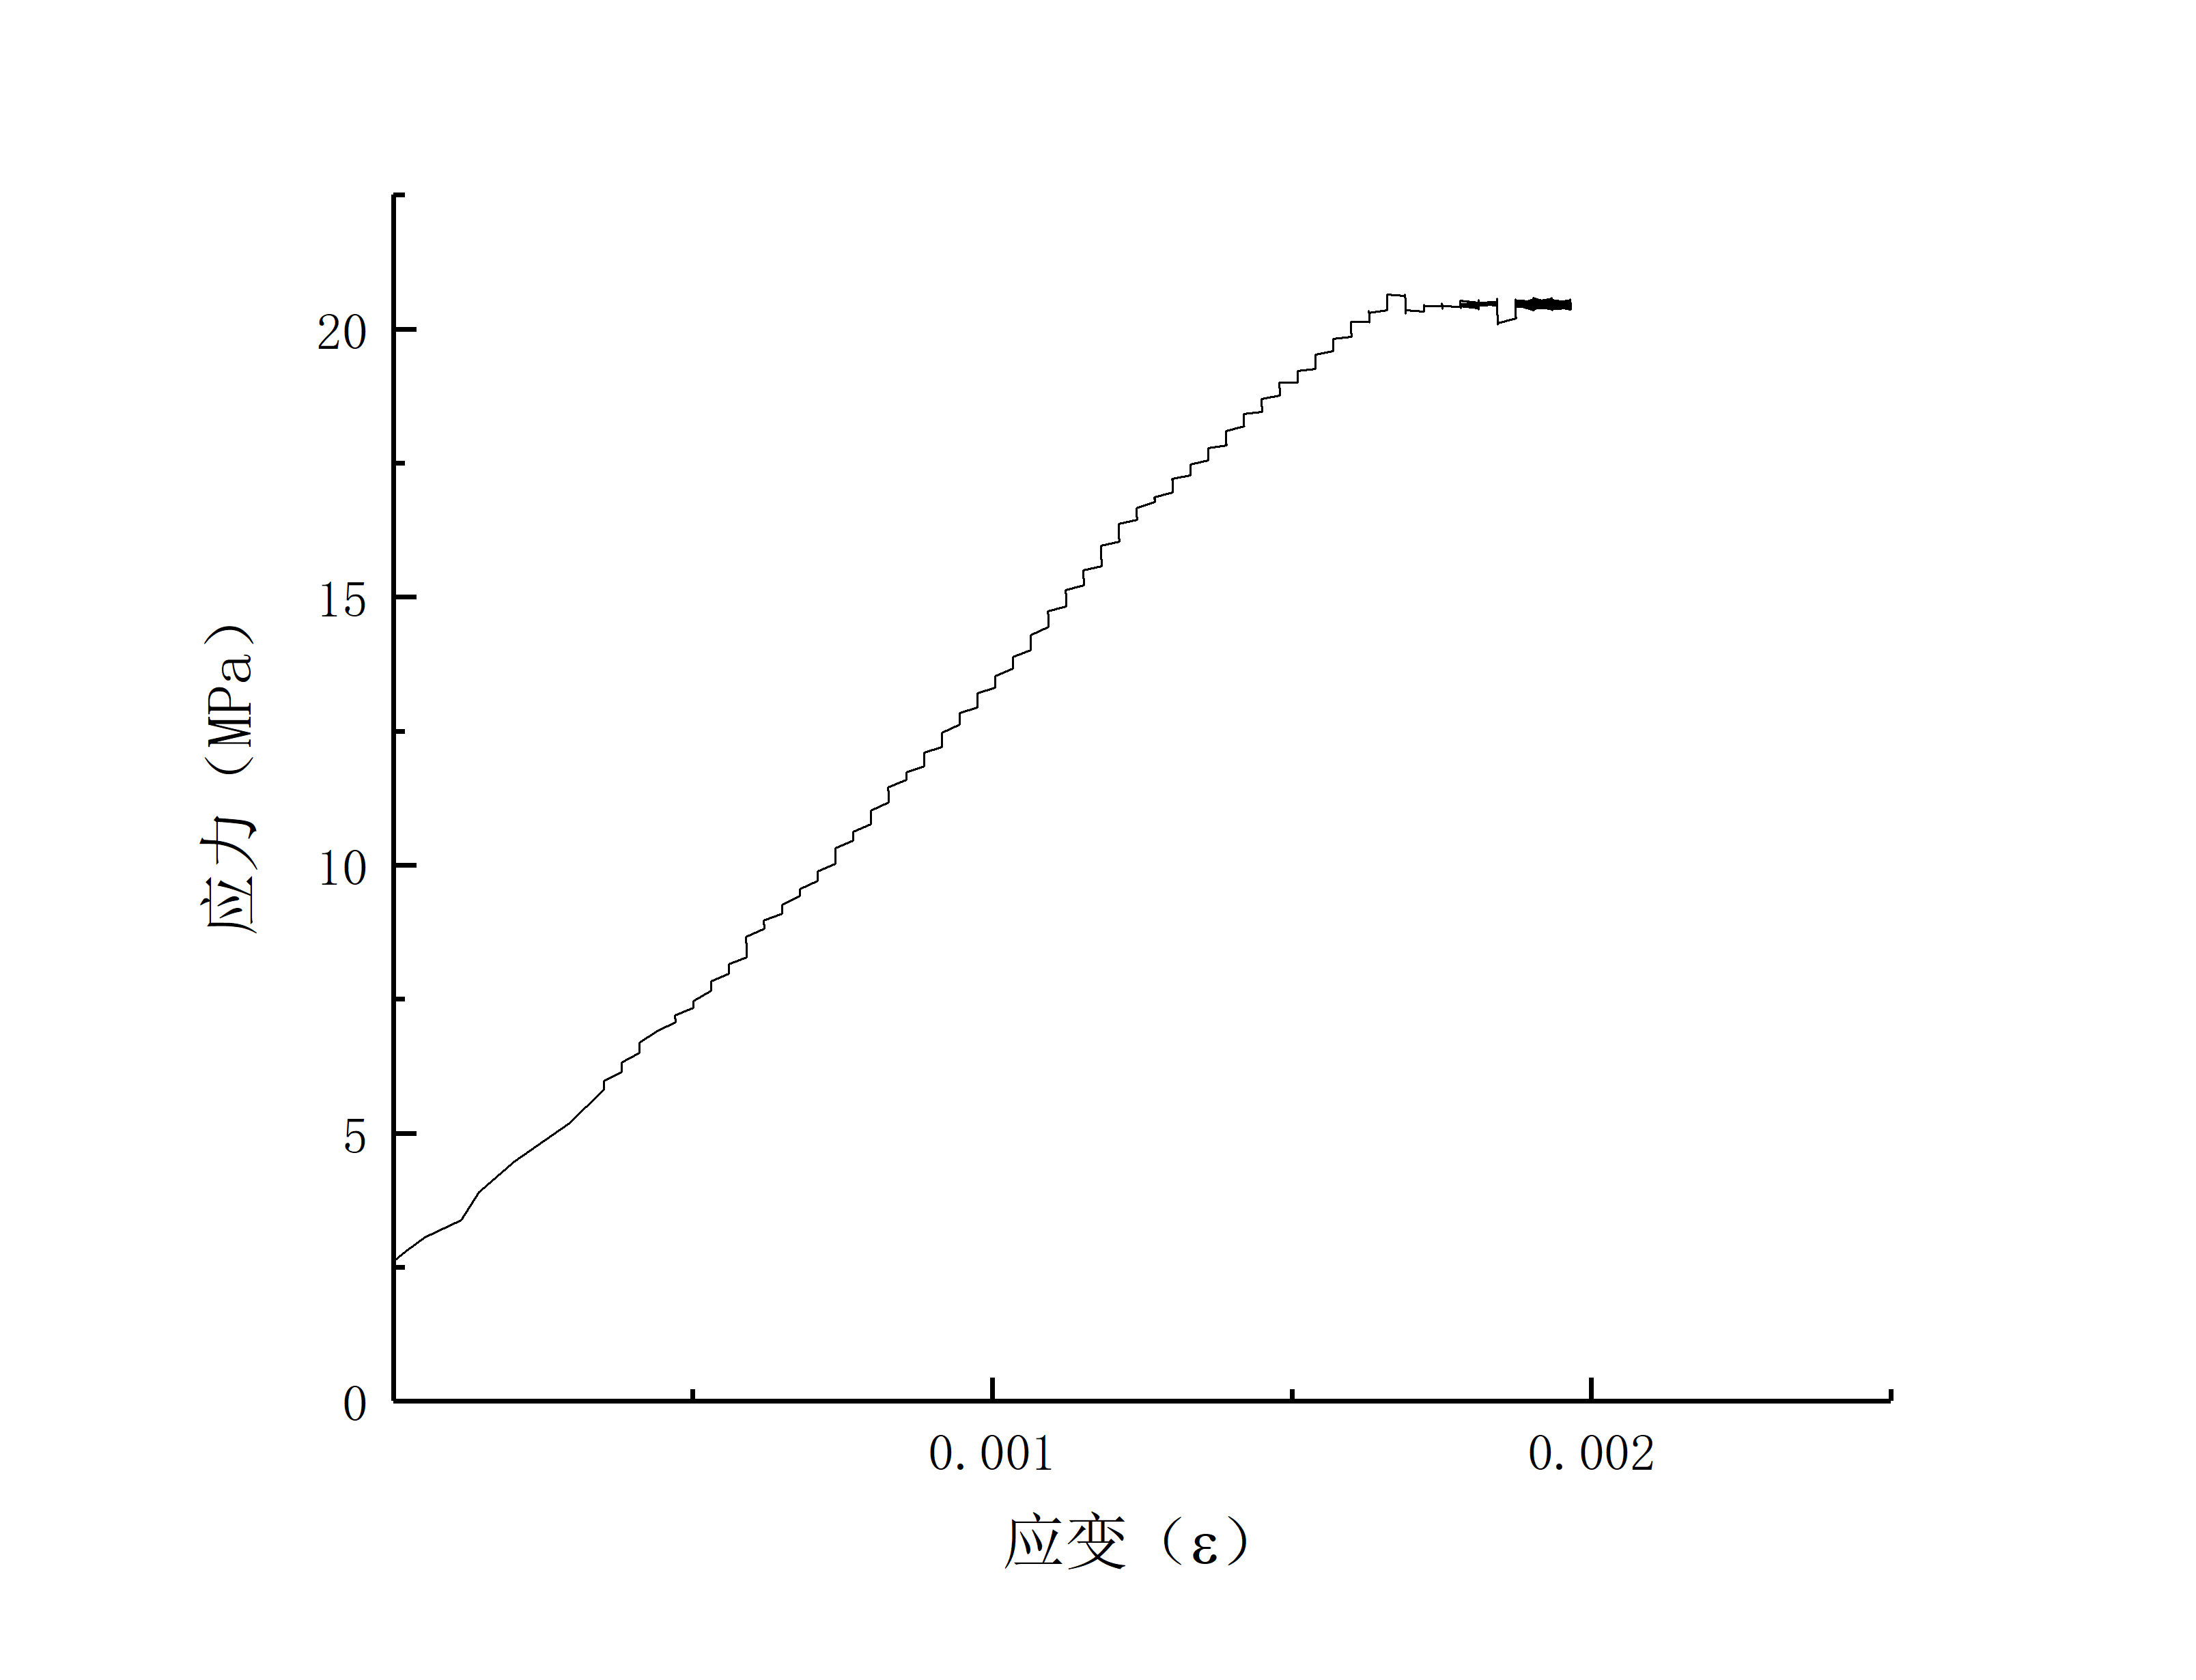
\includegraphics[width=1.1\textwidth]{img/chap2/stress-strain-C05.png}
        \end{minipage}
    }
    \centering
    \caption{单轴流变应力-应变曲线图}
    \label{fig:2-14}
\end{figure}

\section{岩石流变破裂机制探讨}
\subsection{岩石流变破裂形式}

泥岩单轴流变试验中五组试样的流变破坏形态如图\ref{fig:2-6}所示,试样在流变作用下裂纹得到充分扩展,基本表现为斜拉裂缝,局部表现为剪切破坏。而随着加载应力的增大,相应的试样上出现的裂缝也越多,说明荷载越大,流变破坏越明显。在五组试样中仅有C-03试样发生了破坏,其余四组试样仅出现了裂缝,并未完全破坏。
\begin{figure}[ht!]
    \centering
    \subfigure[C-01]
    {
        \begin{minipage}{6cm}
            \centering
            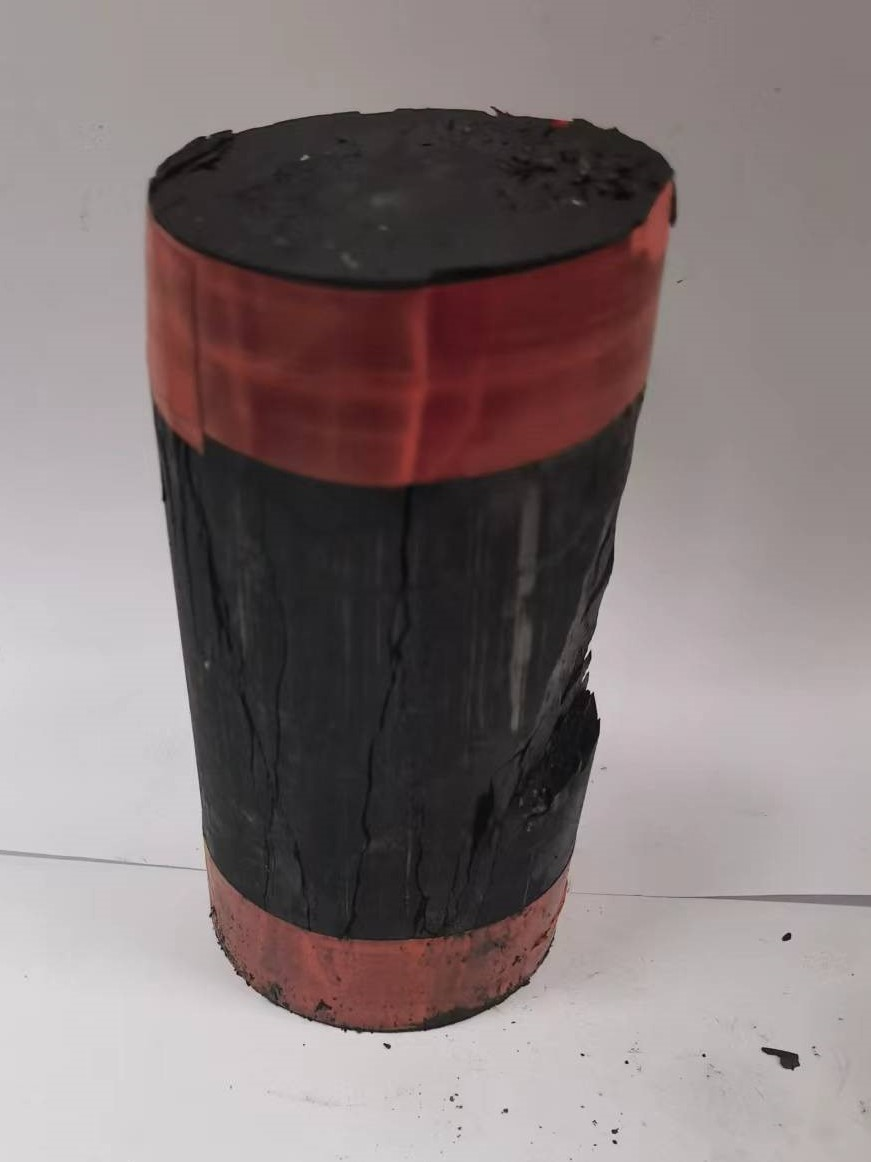
\includegraphics[width=0.9\textwidth]{img/chap2/C-1.jpg}
        \end{minipage}
    }
    \subfigure[C-02]
    {
        \begin{minipage}{6cm}
            \centering
            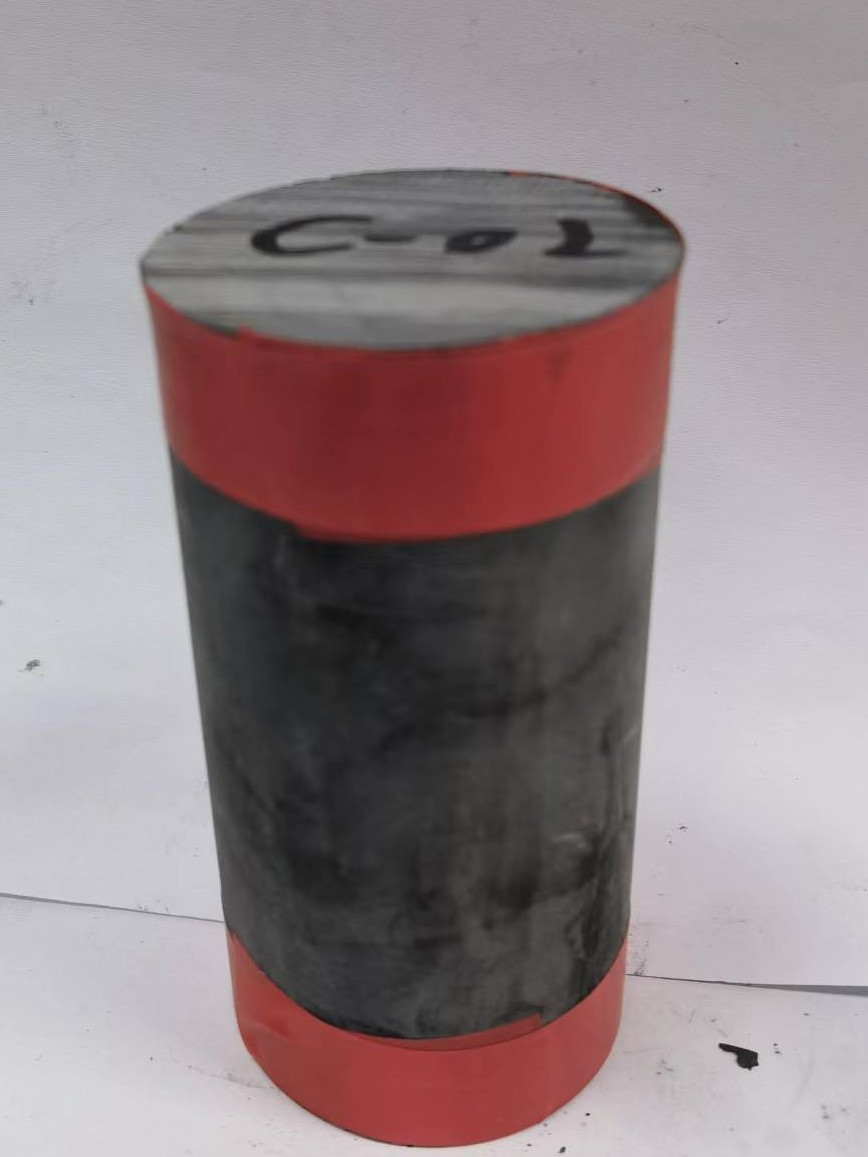
\includegraphics[width=0.9\textwidth]{img/chap2/C-2.jpg}
        \end{minipage}
    }
	
    \subfigure[C-03]
    {
        \begin{minipage}{6cm}
            \centering
            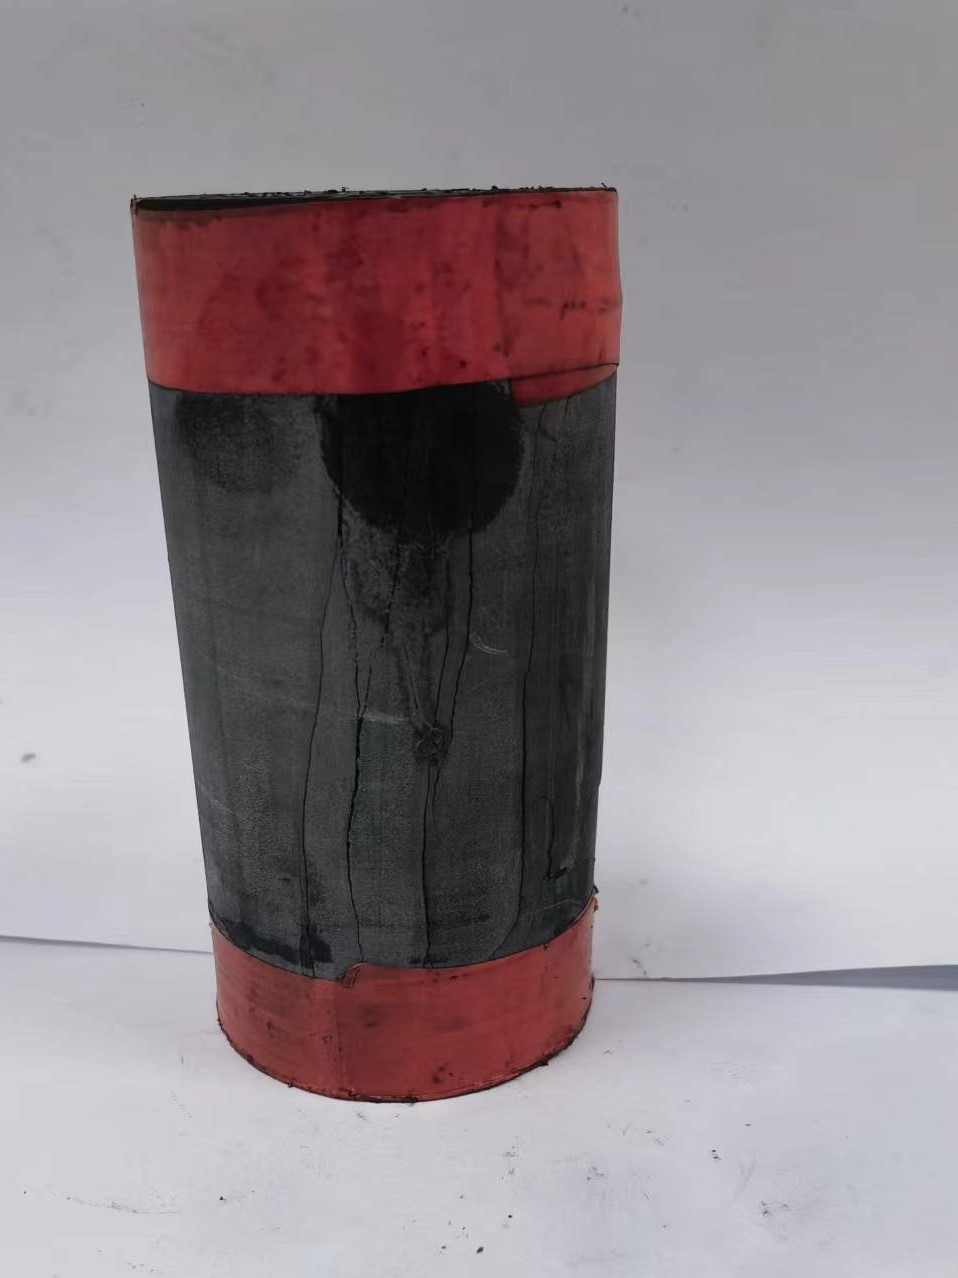
\includegraphics[width=0.9\textwidth]{img/chap2/C-3.jpg}
        \end{minipage}
    }
    \subfigure[C-04]
    {
        \begin{minipage}{6cm}
            \centering
            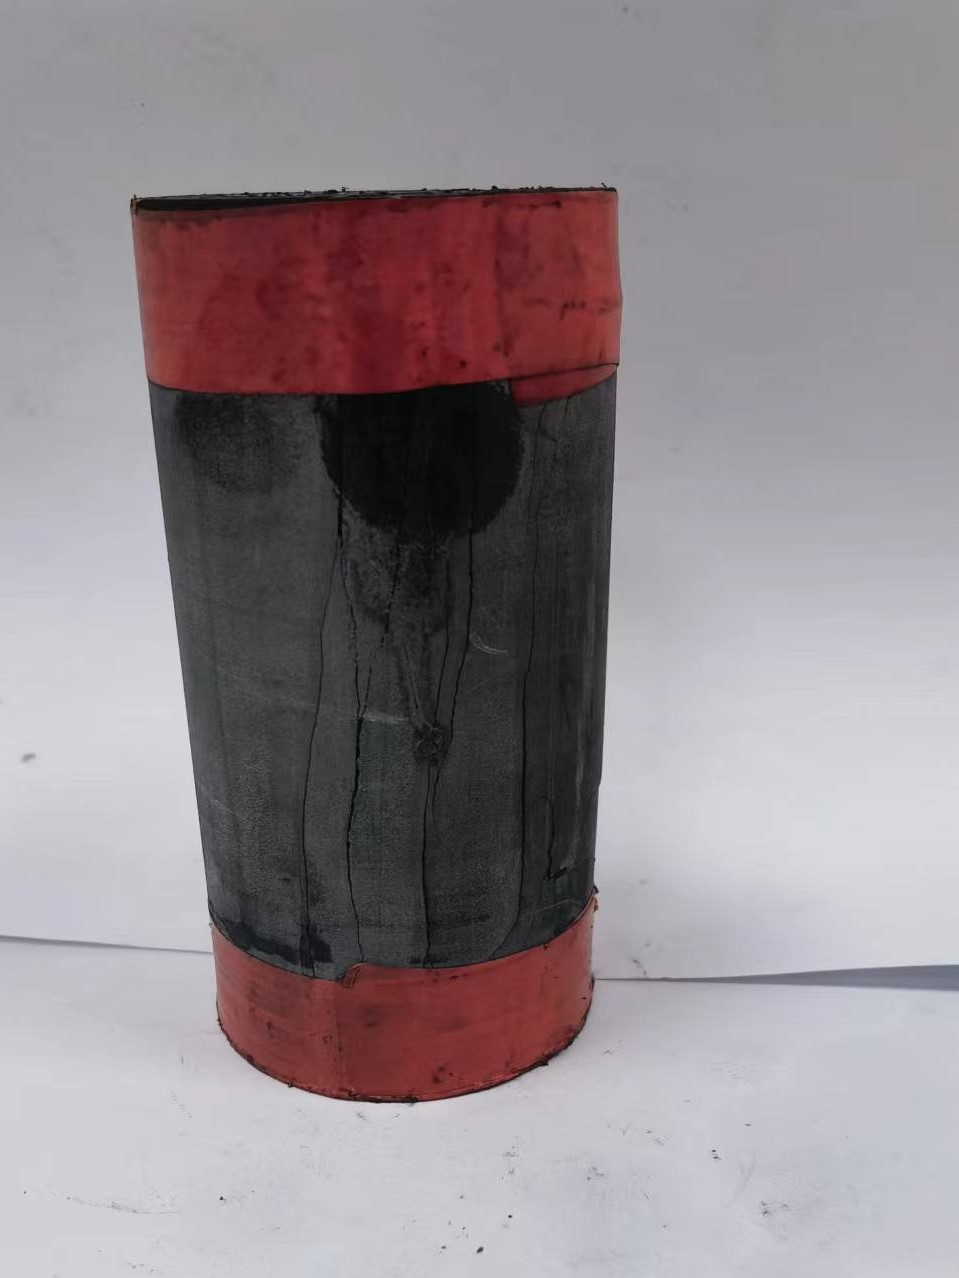
\includegraphics[width=0.9\textwidth]{img/chap2/C-4.jpg}
        \end{minipage}
    }
    \centering
    \subfigure[C-05]
    {
        \begin{minipage}{6cm}
            \centering
            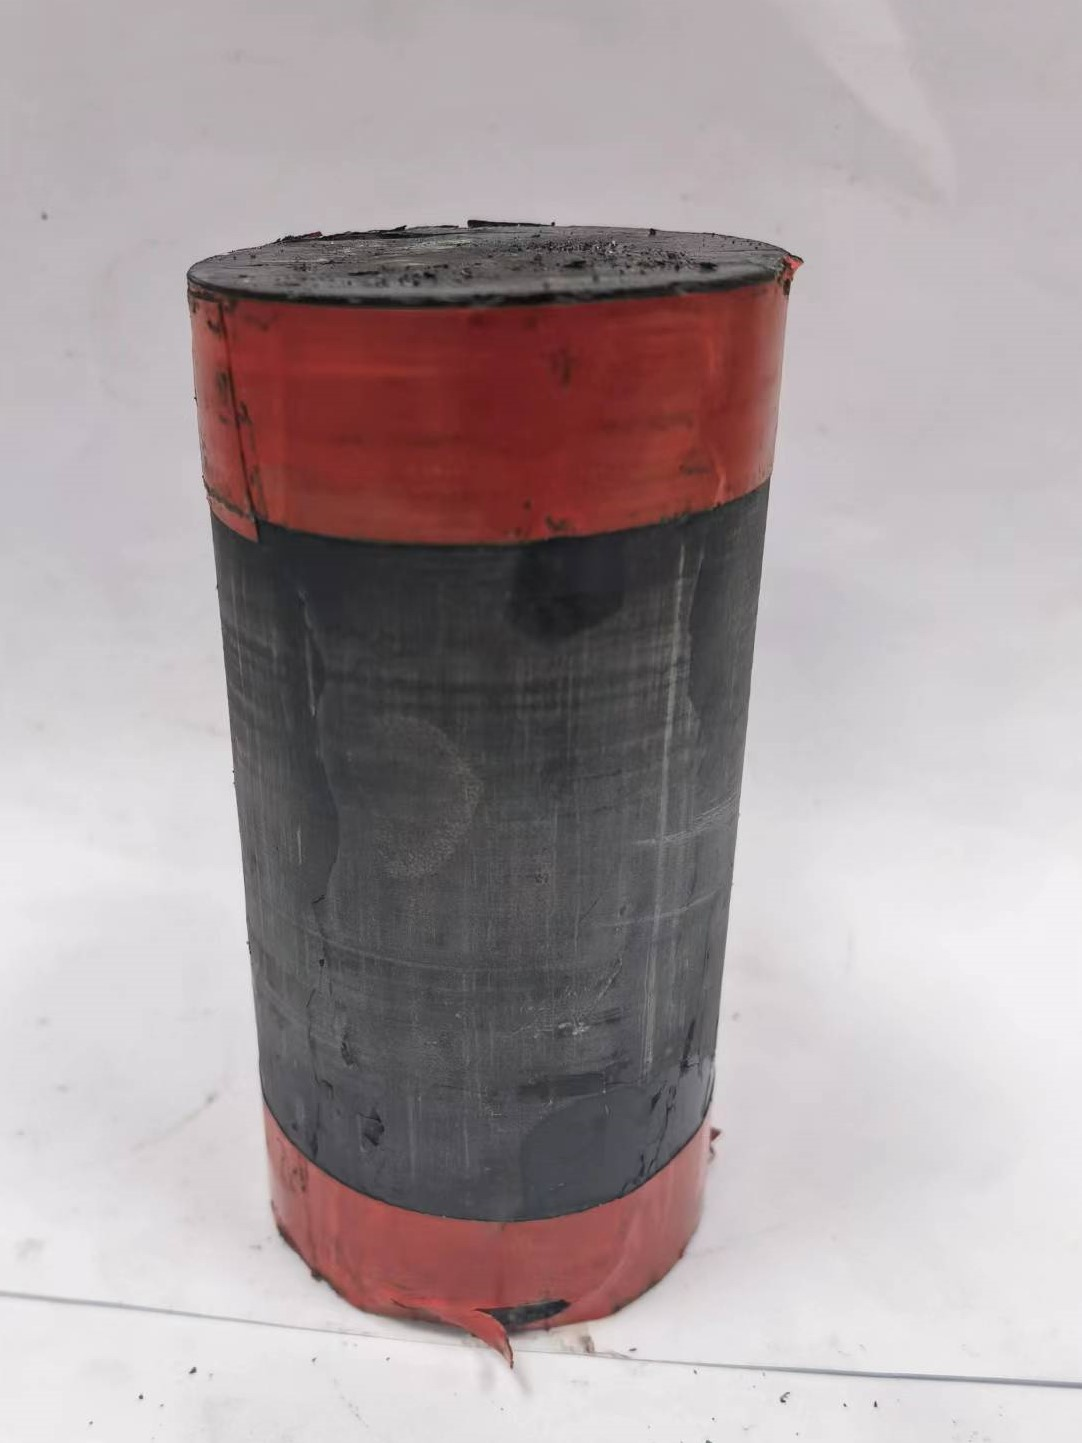
\includegraphics[width=0.9\textwidth]{img/chap2/C-5.jpg}
        \end{minipage}
    }
    \centering
    \caption{泥岩试样单轴流变破裂形式}
    \label{fig:2-6}
\end{figure}

而如图\ref{fig:2-7},在三轴流变试验中,三组试样在分级加载下均发生了结构破坏,从破坏后的试样可以看出,试验过程中均发生了剪切破坏,并伴随有部分次生剪切裂纹。在稳定蠕变阶段,裂纹以极其微弱的速度增长,主裂纹宽度有所增加,同时在试样主裂纹附近产生新的细小裂纹。在加速蠕变阶段,试样表面宏观裂纹开始互相贯通,膨胀扩容现象明显,由裂纹交织形成的细小碎片从母岩脱落。当主裂纹完全贯通,试样破坏,由动能释放产生的声响较大。

在流变试验中,裂纹的开裂扩展实质是能量耗散的过程。对岩石所做的功除累积于岩石内部的势能外,一部分在开裂过程在以粘性效应和摩擦热消耗掉,一部分以动能的形式由位错和裂纹扩展释放,常常以声发射或蠕变曲线的不规则跳动表现出来。

\begin{figure}[ht!]
    \centering
    \subfigure[D-01]
    {
        \begin{minipage}{6cm}
            \centering
            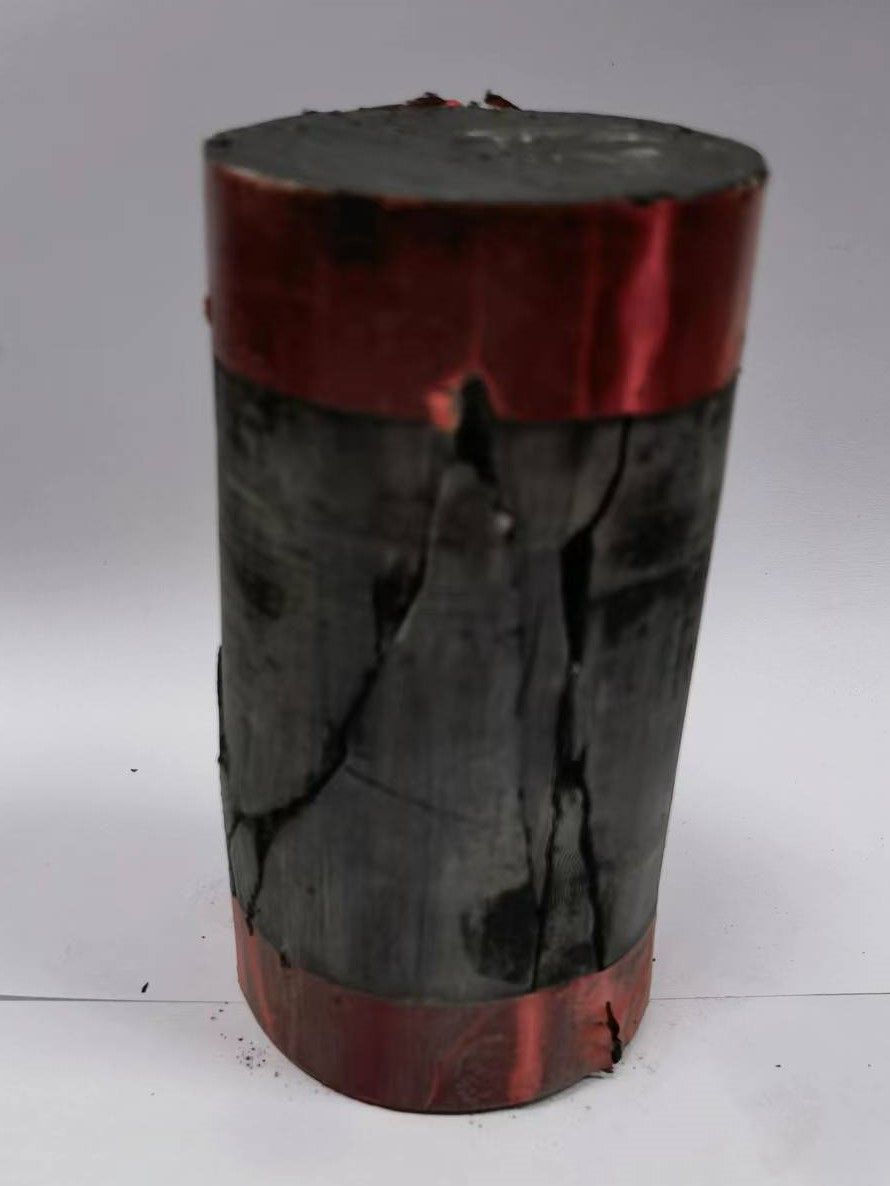
\includegraphics[width=1\textwidth]{img/chap2/D-1.jpg}
        \end{minipage}
    }
    \subfigure[D-02]
    {
        \begin{minipage}{6cm}
            \centering
            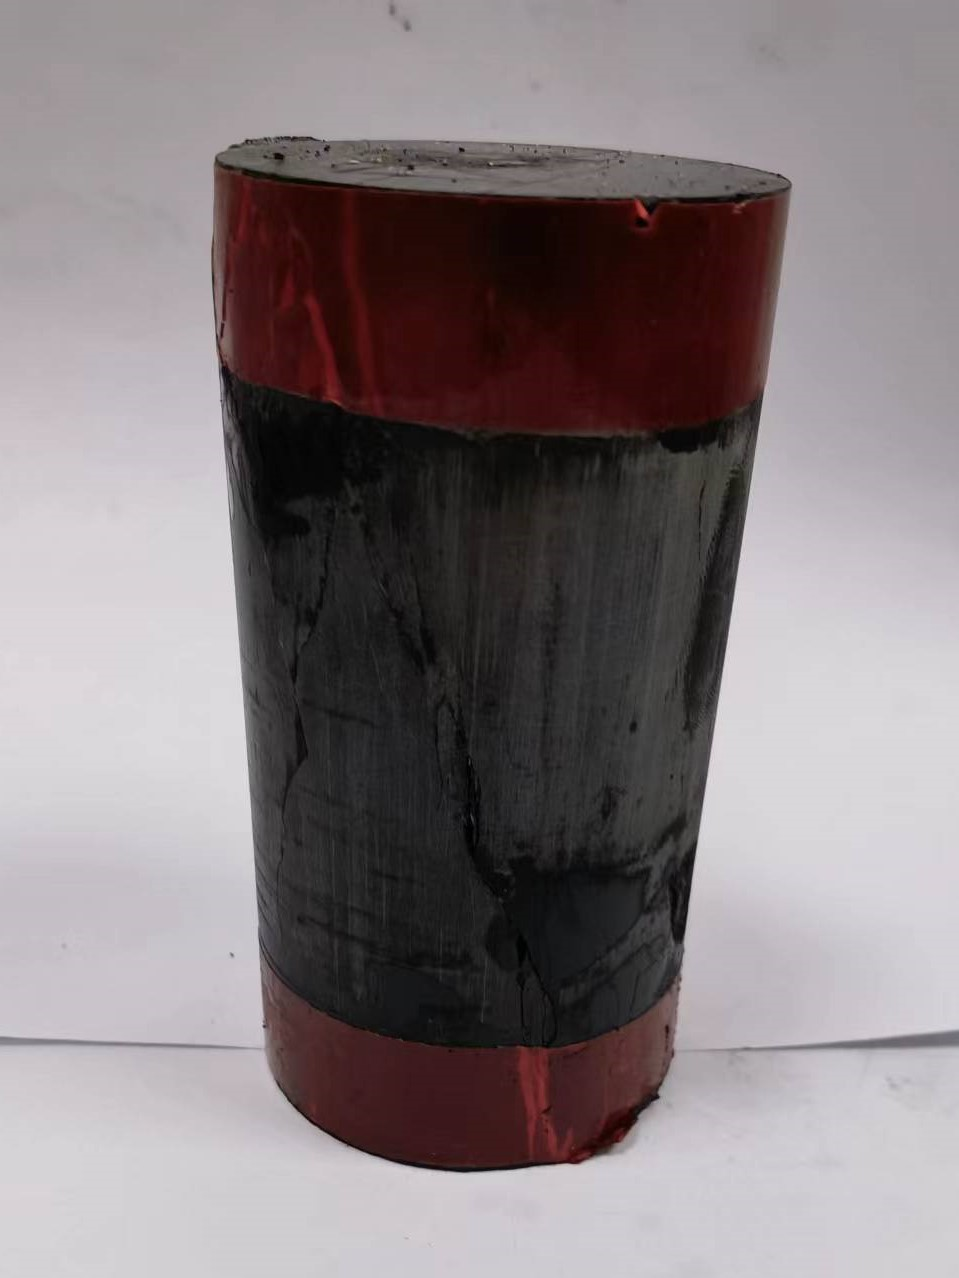
\includegraphics[width=1\textwidth]{img/chap2/D-2.jpg}
        \end{minipage}
    }
	
    \subfigure[D-03]
    {
        \begin{minipage}{6cm}
            \centering
            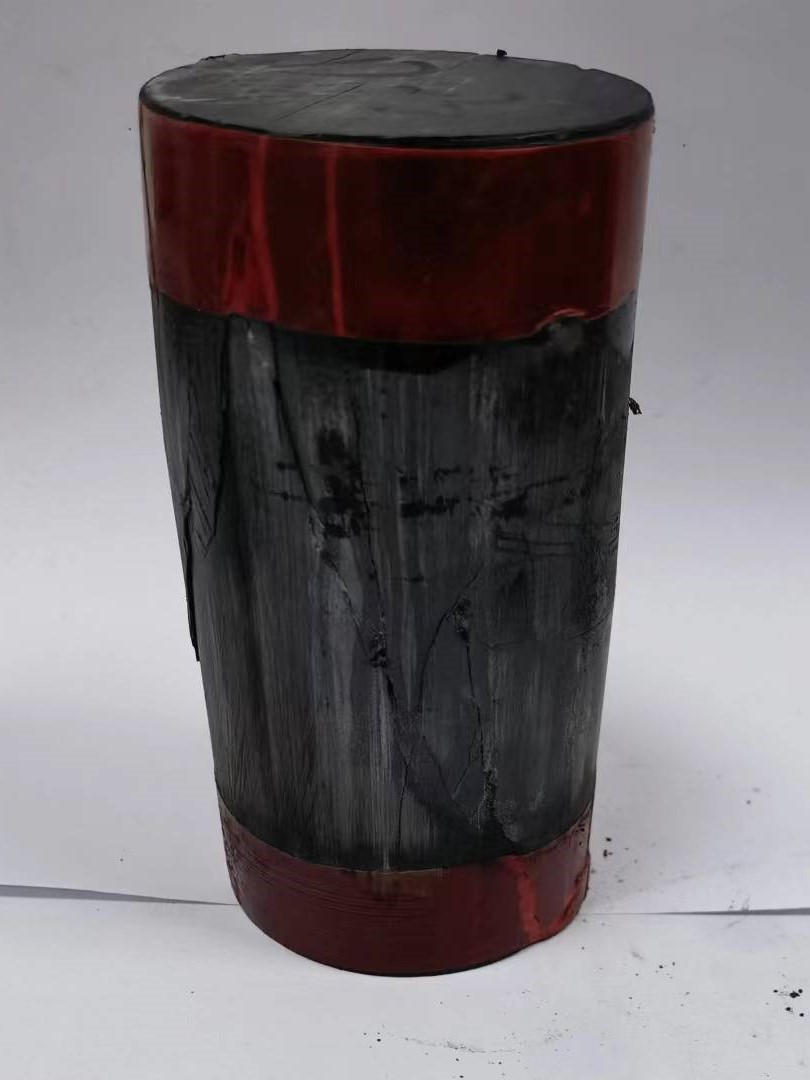
\includegraphics[width=1\textwidth]{img/chap2/D-3.jpg}
        \end{minipage}
    }
    \centering
    \caption{泥岩三轴流变破坏形式}
    \label{fig:2-7}
\end{figure}

\subsection{泥岩微观流变破裂机制探讨}

上一节阐述了试样宏观上的破坏形式,然而该过程只占整个流变全过程很短的时间,大部分时间均为岩石内部微裂纹、微结构变化发展的过程,这也是形成宏观裂纹的前提,要深入分析岩石流变破坏就必须对微裂纹、微结构的演化机理分析研究。

对于流变损伤断裂的研究多见于金属等晶体的变形过程。晶体在位错滑移过程中遇到障碍物塞积,产生硬化,同时在位错塞积群附近发生应力集中,产生张性裂纹。外力的驱动也可能使晶粒内发生空位扩散,空位绕晶粒边界扩散或穿晶扩散。岩石作为一种多晶复合介质,与金属的流变损伤机制有所不同,可将其内部划分为三种类型:晶粒内部、晶粒界面、晶粒间隙。晶粒由于扩散蠕变而变形并沿粘性晶界互相滑动,晶界处微孔由于空位扩散而成核,并汇集成断裂轨迹。微孔成核过程中一些物质扩散并淤积于晶粒边界,削弱晶粒间的联结,形成“蚀变带”。晶界上微孔成核的过程即为材料流变损伤的过程。

不同种类的岩石,由于组成结构不同,其微细观流变破裂机制有所差别。泥岩中黏土颗粒含量较高,这些细小的黏土颗粒构成了较大的集粒,相互交织定向排列,呈絮凝状结构,单元体以细小颗粒构成了较大的集粒,
它们相互交织呈定向排列,这种结构反映了泥岩主要由黏土矿物组成的特性,其孔隙存在于絮凝状结构之间,分布较为均匀。

在初始蠕变阶段,泥岩中的粗粒晶体几乎不产生变形及位错滑移,主要为初始微孔、微裂纹的闭合,黏土类胶结物被压缩咬合,泥岩得到硬化,结构强度提高。在第二蠕变阶段,黏土类胶结物出现弱化,微孔、微裂纹开始等速扩展,结构破坏逐渐增多,应力不断调整。在此阶段虽然损伤不断发展,但是结构硬化和损伤始终保持动态平衡。在加速蠕变阶段,黏土类胶结物被破坏,黏土物质与粗粒晶体分离并形成空洞,晶体颗粒互相错动,结构大量破坏。此时损伤积累完成并呈现加速发展,当由微缺陷组成的裂隙贯通时,岩样发生破坏。

岩石的蠕变破坏过程就是岩石内部应力不断调整的过程,也是硬化与软化相互作用的过程。在蠕变初始阶段,微孔隙闭合、软弱相的压缩及颗粒协调变形使岩石强度提高,硬化占据主要地位。在第二蠕变阶段,随着微裂隙的扩展损伤逐步积累,软弱相破坏退出工作,应力不断调整,蠕变规律随损伤速率等速变化。在第三蠕变阶段,微裂隙累积形成宏观细裂纹并贯通形成主裂面,损伤呈非线性加速发展,岩石蠕变破坏。


\section{小结}
本试验以泥岩为研究对象,通过开展常规单轴、三轴压缩试验获得泥岩的基本物理参数,再通过室内单、三轴流变试验研究泥岩的流变特性,得出的主要结论如下:

(1)通过开展常规单、三轴压缩试验,发现泥岩应力—应变曲线三个主要阶段——弹性变形阶段、微裂隙发展阶段、破坏阶段的变形特征,得到了泥岩的弹性模量、泊松比等基本物理参数。泥岩试样在常规压缩试验下的破化特征主要呈现出纵向的劈裂、张拉破坏以及局部的剪切破坏,而泥岩在流变试验下呈现出的主要为剪切破坏形态。

(2)通过对Boltzmann叠加原理对三轴流变试验的阶梯型流变曲线进行处理。

(3)通过处理完成的单、三轴流变试验的时间-应变曲线,我们可以发现流变变形量随应力等级的提高而增加,随着应力等级的提高,泥岩的流变变形量以及残余应变值也在逐渐增加。在本次试验中,岩泥在加载瞬间产生的瞬时变形,随后进入衰减和稳定蠕变的阶段,稳定蠕变阶段历史最长但流变变形量小。
试验时施加的应力越大,初始流变速率及稳态流变速率也呈递增趋势,流变速率在初始蠕变阶段内不断减小,在稳定蠕变阶段达到一个保持不变的数值,在较低的应力下,稳定蠕变速率将会无限接近于0。

(4)本次实验中,在单轴流变实验中未出现加速蠕变阶段。在三组三轴流变试验中,在最后一级应力加载下均出现了加速蠕变阶段,加速蠕变阶段虽然流变历时较短,但流变变形量远大于前几级应力下的流变量。

(5)岩石试样的破裂形式主要表现为轴向张拉破坏,局部表现为剪切破坏。宏观破坏主要集中在加速蠕变阶段,裂纹互相交织形成贯通试样的破裂面,膨胀扩容变形现象明显。微观条件下,初始微缺陷产生的位错、滑移与晶体颗粒协调变形构成软化与硬化两种机制相互竞争的局面。当内部微缺陷、微裂纹由于长期损伤积累已经占据主要地位时,原有胶结结构破坏,黏聚力丧失,损伤呈非线性加速发展,微裂纹汇聚形成宏观裂纹,岩石蠕变破坏。









